
\documentclass{report}
    \title{Statistical Signal Processing \& Inference notes}
    \author{Timothy Chung}
    \date{8/01/24}
    
    \usepackage[a4paper, total={7in, 10in}]{geometry}
    \setlength\parindent{0pt}
    %=======================PACKAGES FOR NEWCOMMAND CREATION========================
\usepackage{xparse}
%===============================================================================

%=========================PACKAGES FOR USE IN DOCUMENT==========================
\usepackage[dvipsnames]{xcolor}
\usepackage{graphicx, amssymb, amsfonts, amsmath, listings, multirow, hyperref, mathtools, svg, tikz, enumitem, minted, xfrac, multicol}
\usepackage[most]{tcolorbox}
\usepackage[super]{nth}
\usepackage{tabularx}  % for 'X' column type
\usepackage{multirow}  % for multirow cells
\usepackage{pgfplots}
\pgfplotsset{compat=1.18}
\usetikzlibrary{calc, shapes.geometric, arrows.meta, positioning}

\tikzset{
    neuron/.style={circle, draw, minimum size=1cm},
    input neuron/.style={neuron, fill=gray!20},
    output neuron/.style={neuron, fill=gray!60},
    activation function/.style={
        rectangle,
        draw,
        minimum size=1cm,
        fill=gray!30,
        path picture={
            % Draw the step function inside the activation function node
            \draw[thick] 
            ($(path picture bounding box.south)+(-0.3cm,0.2cm)$) -- 
            ($(path picture bounding box.south)+(0cm,0.2cm)$) -- 
            ($(path picture bounding box.south)+(0cm,0.7cm)$) -- 
            ($(path picture bounding box.south)+(0.3cm,0.7cm)$);
        }
    },
    arrow label/.style={midway, above}
}


% ======= CUSTOM 
\usepackage{subcaption}
\usepackage{wasysym}

%=================================GLOBAL SETUP==================================
\setitemize{itemsep=0em}
%===============================================================================

%===============================INCLUDE CHAPTERS================================
\newcommand{\addchapter}[1]{\include{#1/#1}}
%===============================================================================

%==============================UNFINISHED SECTION===============================
\newcommand{\unfinished}{\begin{huge} \textcolor{red}{\textbf{UNFINISHED!!!}} \end{huge}}
\newcommand{\toimprove}{\begin{huge} \textcolor{olive}{\textbf{NEEDS IMPROVEMENT!!!}} \end{huge}}
%===============================================================================

%==============================PAGE SPLIT LAYOUTS===============================
\NewDocumentCommand{\twosplit}{O{0.48} O{#1} m m}{
	\begin{minipage}[t]{#1\textwidth}
		#3
	\end{minipage}
	\hfill
	\begin{minipage}[t]{#2\textwidth}
		#4
	\end{minipage}
}
%===============================================================================

%============================SPECIAL COLOURED BOXES=============================

% For term definitions
% \begin{definitionbox}{term}
%	... the term's definition ...
% \end{definitionbox}
\newtcolorbox[auto counter,number within=section]{definitionbox}[2][]{%
	colback=blue!5!white,colframe=blue!75!black,arc=0mm,sharp corners=all,fonttitle=\bfseries,%
	title=#2 \hfill Definition \thetcbcounter #1}

% For term definitions
% \begin{sidenotebox}{cool title}
%	... cool unsassessed/not required info ...
% \end{sidenotebox}
\newtcolorbox[auto counter,number within=section]{sidenotebox}[2][]{%
	colback=black!5!white,colframe=black!75!black,arc=0mm,sharp corners=all,fonttitle=\bfseries,%
	title=#2 \hfill \textit{Extra, Not Assessed} \thetcbcounter #1}
% previously the text was "Extra Fun!"

% For example questions:
% \begin{examplebox}{question name}
%   ... the question ...
%	\tcblower
%   ... the worked answer ...
% \end{examplebox}
\newtcolorbox[auto counter,number within=section]{examplebox}[2][]{%
	colback=orange!5!white,breakable,colframe=orange!75!black,arc=0mm,sharp corners=all,fonttitle=\bfseries,%
	title=#2 \hfill Example Question \thetcbcounter #1}

% For exam questions (no answers):
% \begin{exambox}{1c}{2018}
%   ... the question ...
% \end{exambox}
\newtcolorbox[auto counter,number within=section]{exambox}[3][]{%
	colback=purple!5!white,breakable,colframe=purple!75!black,arc=0mm,sharp corners=all,fonttitle=\bfseries,
	title=Q#2 - #3 \hfill Exam Question \thetcbcounter #1}

% For comments:
% \begin{commentbox}
%   ... the question ...
% \end{commentbox}
 
\newtcolorbox[auto counter,number within=section]{commentbox}[2][]{%
    colback=orange!5!white,
    colframe=orange!95!black, % Darker orange frame
    coltitle=white, % White title text
    arc=0mm,
    sharp corners=all,
    fonttitle=\bfseries,
    title=#2 \hfill
}


 

% For positives/pros 
% \begin{prosbox}
%	... the term's definition ...
% \end{prosbox}
\newtcolorbox[]{prosbox}[1][]{%
	colback=green!5!white,breakable,colframe=green!75!black,leftrule=3mm,arc=0mm,sharp corners=all, #1}

% For negatives/cons 
% \begin{prosbox}
%	... the term's definition ...
% \end{prosbox}
\newtcolorbox[]{consbox}[1][]{%
	colback=red!5!white,breakable,colframe=red!75!black,leftrule=3mm,arc=0mm,sharp corners=all, #1}

% For negatives/cons 
% \begin{tabbox}{consbox}
%	... the term's definition ...
% \end{tabbox}
\newenvironment{tabbox}[2][.8\textwidth]{
	\def\boxtype{#2}
	\begin{\boxtype}
		\begin{center}
			\begin{tabular}{r p{#1}}
				}{
			\end{tabular}
		\end{center}
	\end{\boxtype}
}

% \begin{panoptobox}
%   ... the question ...
% \end{panoptobox}
\newtcolorbox{panoptobox}{enhanced,arc=0mm,breakable,sharp corners=all,colback=gray!5,colframe=gray,leftrule=12mm,detach title,%
	underlay unbroken and first={\node[below,text=black,anchor=east] at (interior.base west) {\includegraphics[width=11mm]{../common/images/panopto_logo.png}};}}

\newcommand{\lectlink}[2]{
	\begin{panoptobox}
		\textbf{\href{#1}{#2}}
	\end{panoptobox}
}


% For theorems:
% \begin{theorembox}
%   ... the question ...
% \end{theorembox}
 
\newtcolorbox[auto counter,number within=section]{theorembox}[2][]{%
    colback=red!5!white,
    colframe=red!95!black, % Darker orange frame
    coltitle=white, % White title text
    arc=0mm,
    sharp corners=all,
    fonttitle=\bfseries,
    title=#2 \hfill Theorem \thetcbcounter #1
}


%===============================================================================
    \newcommand{\infer}[2]{\cfrac{#1}{#2}}
    \newcommand{\infers}[3]{\cfrac{#1}{#2}(#3)}
    
    \newcommand{\ninfer}[3]{(\text{#1}):\cfrac{#2}{#3}}
    \newcommand{\ninfers}[4]{(\text{#1}):\cfrac{#2}{#3}(#4)}
    \newcommand{\ainfer}[3]{\cfrac{#2}{#3}(\text{#1})}
    
    \newcommand{\mllet}[2]{\text{let } #1 \text{ in } #2}
    \newcommand{\mlfix}[2]{\text{fix } #1 . #2}
    
    \newcommand{\hc}{\mathcal{H}}
    \newcommand{\cov}{\text{Cov}}
    \newcommand{\E}{\text{E}}
    \newcommand{\var}{\text{Var}}
    \newcommand{\mb}{\mathbf}
    \newcommand{\est}{\hat{\theta}}
    \newcommand{\p}{\theta}
    
    
    
\begin{document}
\include{titlepage/titlepage}
\setlength{\cftsecnumwidth}{4.2em} 

\begin{titlepage}
\centering
    \vspace*{1cm}
    \Huge
    \textbf{BUSI60040 Corporate Finance} \\
    \vspace{1cm}
    \Large
    Timothy Chung \\
    \vspace{1cm}
    Spring 2024 \\
    \vfill
\end{titlepage}

\setcounter{tocdepth}{1}
\tableofcontents
\newpage
\setcounter{chapter}{-1}
\chapter{Foreword}
The notes are intended to keep a rough track of the (rather lacking) syllabus found on the website \href{https://www.imperial.ac.uk/business-school/undergraduate/bpes/#programme-content}{here.} The notes here themselves are far from a proper curruiculum in corporate finance, more interested readers can consult a better textbook \href{https://book.ivo-welch.info/home/}{here}. \\

This module aims to give an overview of the two key financial instruments: Stocks and Bonds. It will also introduce the key derivatives marketing: Futures and  Options. You will be introduced to the concepts of risk and return in  financial markers  and how diversification influences risk and return. This module will explore the concept of the cost capital and how it can be calculated. You will learn how companies are financed and how to decide between different sources of finance. 

\sn{On The Rigour of A Random Variable}{
For the beginning of this module, a random variable $X$ is considered to be a function from a sample space $\Omega$ to the unit interval $[0, 1]$. However, in Lectures 6 and 7, we use the full definition of a random variable, which is a measurable function from a sample probability space $(\Omega)$ to a measurable space $(E, \varepsilon)$, involving the concept of $\sigma$-algebras and measure spaces. \bigskip

When the sample space is a continuous space, the function $p$ is a \textbf{probability density function} (PDF). When the sample space is a discrete space, the function $p$ is a \textbf{probability mass function} (PMF).
} 


\marginnote[-60pt]{We will introduce measure theory later.}





\section{Brief Probability Theory Review}

$x$ is a sample from a random variable $X$. 

\noindent $P(X=x)$ refers to probability that the random variable $X$ takes on the value $x$.

\subsection{Probability Density Function (PDF)}
\begin{marginfigure}[100pt]
    \centering
    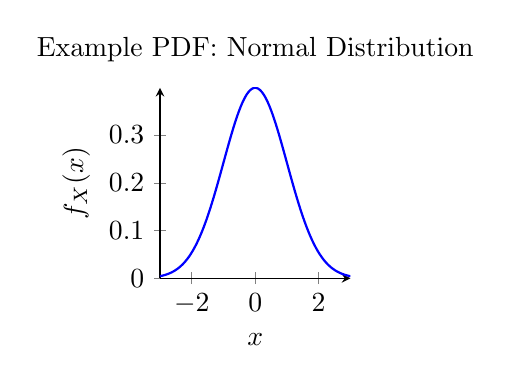
\begin{tikzpicture}
        \begin{axis}[
            width=4cm,
            height=4cm,
            xlabel={$x$},
            ylabel={$f_X(x)$},
            domain=-3:3,
            samples=100,
            axis lines=left,
            ymin=0,
            legend pos=north east,
            title={Example PDF: Normal Distribution}
        ]
        \addplot[blue, thick] {exp(-x^2 / 2) / sqrt(2 * pi)};
        \end{axis}
    \end{tikzpicture}
    \caption{Probability Density Function of a standard normal distribution}
\end{marginfigure}

The Probability Density Function (PDF) of a continuous random variable \(X\) is a function \(f_X(x)\) that describes the relative likelihood for this random variable to take on a given value. The PDF has the following properties:
\begin{itemize}
    \item \(f_X(x) \geq 0\) for all \(x\).
    \item \(\int_{-\infty}^{\infty} f_X(x) \, dx = 1\).
\end{itemize}

Mathematically, the PDF is defined such that the probability that \(X\) lies within a particular interval \([a, b]\) is given by:
\[
P(a \leq X \leq b) = \int_{a}^{b} f_X(x) \, dx.
\]


\subsection{Cumulative Distribution Function (CDF)}
\begin{marginfigure}[50pt]
    \centering
    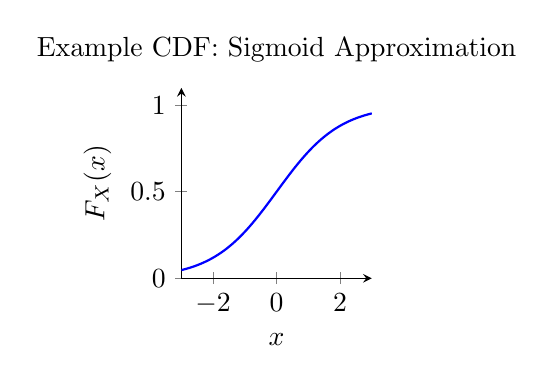
\begin{tikzpicture}
        \begin{axis}[
          width=4cm,
          height=4cm,
            xlabel={$x$},
            ylabel={$F_X(x)$},
            domain=-3:3,
            samples=100,
            axis lines=left,
            ymin=0, ymax=1.1,
            legend pos=south east,
            title={Example CDF: Sigmoid Approximation}
        ]
        \addplot[blue, thick] {1 / (1 + exp(-x))};
        \end{axis}
    \end{tikzpicture}
    \caption{Cumulative Distribution Function}
\end{marginfigure}

The Cumulative Distribution Function (CDF) of a continuous random variable \(X\) is a function \(F_X(x)\) that describes the probability that \(X\) will take a value less than or equal to \(x\). It is defined as:
\[
F_X(x) = P(X \leq x) = \int_{-\infty}^{x} f_X(t) \, dt.
\]

The CDF has the following properties:
\begin{itemize}
    \item \(0 \leq F_X(x) \leq 1\) for all \(x\).
    \item \(F_X(x)\) is a non-decreasing function.
    \item \(\lim_{x \to -\infty} F_X(x) = 0\).
    \item \(\lim_{x \to \infty} F_X(x) = 1\).
\end{itemize}


\subsection{Dealing with Data (Single-Feature)}

In Machine Learning (ML), we often deal with large datasets from which we aim to extract meaningful insights. It is useful to model these data points as random variables:
\[
\{x_1, x_2, \ldots, x_N\}
\]


\noindent We typically model these samples as random variables:

\[
\{x_1 \sim X_1, x_2 \sim X_2, \ldots, x_N \sim X_N\}
\]

\subsection{Vectors of Random Variables}

When dealing with joint random variables, we often represent them as vectors:

\[
\mathbf{X} = (X_1, X_2, X_3) \quad \text{with joint distribution} \quad p_{X_1, X_2, X_3}(x_1, x_2, x_3)
\]

\noindent For a vector of random variables \(\mathbf{X}\) in \( \mathbb{R}^3 \), the joint probability density function is denoted as:

\[
p_{\mathbf{X}}(\mathbf{x}) \quad \text{where} \quad \mathbf{X} \in \mathbb{R}^3
\]
\noindent 
If these are input observations, they are often referred to as "feature vectors."

\subsection{Distinct Random Variables}

We model samples as distinct random variables \sidenote[][-20pt]{\textbf{Why should we model these as distinct random variables? Aren't they all the same thing?} \smallskip

\noindent Despite being identically distributed, distinct random variables allow for capturing dependencies and interactions between different samples.
}:\bigskip

\[
\{x_1 \sim X_1, x_2 \sim X_2, \ldots, x_N \sim X_N\}
\]


\section{Independent and Identically Distributed (i.i.d.) Random Variables}

\marginnote[-50pt]{    \textbf{Why do we model samples as distinct random variables?}

\begin{enumerate}
    \item By treating each sample as a distinct variable, we assume samples are i.i.d, allowing every sample to contribute independently to the likelihood of oberving the data given the model prarameters – so every sample provides unique information to estimate the parameters of the underlying distribution. If we treated all samples as a single random variable, we would lose the granularity of information, leading to a poorer estimate.
    \item Treating samples as distinct allows us to study and model the relationships and dependencies between them.
    \item The assumption of i.i.d follows many results in probability and statistics, such as the Central Limit Theorem, which states that the sum of a large number of i.i.d. random variables is approximately normally distributed. It is also an assumed requirement for a model to generalise. The assumption simplifies the analysis and derivation process, allowing us to use techniques like maximum likelihood estimation (MLE) and empirical risk minimization (ERM).
\end{enumerate}
    }
\subsection{Independence of Random Variables}

Independence refers to the idea that the values or outcomes of one observation in a dataset do not depend on or influence the values of any other observation.\\

For the set of random variables $X_1, X_2, \ldots X_n$, for the collection \[\{x_1 \sim X_1, x_2 \sim X_2, \ldots, x_N \sim X_N\}\]

\noindent we often assume independence, for any subset of observations \(\{X_{i1}, X_{i2}, \ldots, X_{ik}\}\) where \(i_1, i_2, \ldots, i_k \in \{1, 2, \ldots, N\}\), the joint distribution factorises:

\begin{equation}
P(X_{i_1} = x_{i_1}, \ldots, X_{i_k} = x_{i_k}) = P(X_{i_1} = x_{i_1}) \cdot \ldots \cdot P(X_{i_k} = x_{i_k})
\end{equation}

\hl{The joint distribution of the subset is the product of the marginal distributions of the individual random variables.} \bigskip

\textbf{Independence:} The occurrence of any event does not affect the occurrence of others. This is a crucial assumption in many ML models that we will see the usefulness of as early as the next lecture.

\subsection{Identically Distributed Random Variables}

The "identically distributed" part of i.i.d. refers to the idea that all random variables in the sample follow the same probability distribution. That is, they share the same probability density function (pdf) or probability mass function (pmf), depending on whether the data is continuous or discrete. If the set of random variables \(\{X_1, X_2, \ldots, X_n\}\) are identically distributed, then:





\begin{equation}
    f_{X_1}(x) = f_{X_2}(x) = \ldots = f_{X_n}(x) = f_{X}(x)
\end{equation}

\begin{equation}
F_{X_1}(x) = F_{X_2}(x) = \ldots = F_{X_n}(x) = F_{X}(x)
\end{equation}

\noindent This implies that the cumulative distribution function (CDF) is the same for all these random variables.


\section{Statistical Modelling as Curve Fitting}

Machine learning and statistics have significant overlap, and so most concepts studied in this module can be cast as statistical modelling. Consider our random variables:

\begin{equation}
\{x_1 \sim X_1, x_2 \sim X_2, \ldots, x_N \sim X_N\}
\end{equation}

\noindent These random variables can be modelled to fit certain curves that represent the underlying data distribution. 

\subsection{Assumption about the Model}

To proceed with statistical modelling, we make an assumption about the form of the model:

\begin{equation}
P_X(x) \approx \mathcal{N}(x; \theta) \quad \theta := (\mu, \sigma)
\end{equation}

Here, \(P_X(x)\) is approximated by a normal distribution \(\mathcal{N}(x; \theta)\), where \(\theta\) represents the parameters of the distribution, namely the mean \(\mu\) and the standard deviation \(\sigma\). This assumption simplifies the process of modelling the data.

\subsection{Fitting the Model}

The next step is to fit the model to the data. This involves finding the parameter values \(\theta\) that maximize the probability of observing the given data. Mathematically, this is expressed as:

\begin{equation}
\arg \max_{\theta} P(x_1, \ldots, x_N \mid \theta)
\end{equation}

In other words, we adjust the parameters \(\mu\) and \(\sigma\) so that the assumed model best fits the observed data. This process is known as maximum likelihood estimation (MLE).\\











\section{Discrete Random Variables}


\subsection{Bernoulli and Multinoulli Distributions}
\textbf{Bernoulli Distribution:} Outcome with two values (e.g., heads or tails).
\begin{itemize}
    \item Parameter: \(\theta\).
    \item Probabilities: \(P(X = 0) = 1 - \theta\), \(P(X = 1) = \theta\).
\end{itemize}

\textbf{Multinoulli Distribution:} Describes a scenario with multiple possible outcomes, extending the Bernoulli distribution to more than two outcomes.
\begin{itemize}
    \item Parameter: \(\bm{\theta} \in \mathbb{R}^s\) where each \(\theta_i\) represents the probability of the \(i\)-th outcome, and \(\sum_{i=0}^{s-1} \theta_i = 1\).
    \item Probabilities: \(P(X = i) = \theta_i\) for \(i = 0, 1, \ldots, s-1\).
\end{itemize}

\subsection{Binomial and Multinomial Distributions}
\textbf{Binomial Distribution:} \(X \sim \text{Bin}(n, \theta)\).
\begin{itemize}
    \item Probability Mass Function (p.m.f):
    \[
    \text{Bin}(k \mid n, \theta) := \binom{n}{k} \theta^k (1 - \theta)^{n-k}
    \]
    \item Binomial Coefficient:
    \[
    \binom{n}{k} = \frac{n!}{(n - k)!k!}
    \]
    \item Mean: \(n\theta\).
    \item Variance: \(n\theta(1 - \theta)\).
\end{itemize}

\textbf{Multinomial Distribution:} Generalises the binomial distribution for more than two outcomes. It models the probabilities of counts among multiple categories in \(n\) independent trials.
\begin{itemize}
    \item Parameters: \(n\) (number of trials) and \(\boldsymbol{\theta} = (\theta_1, \theta_2, \ldots, \theta_K)\) where \(\theta_i\) is the probability of the \(i\)-th category and \(\sum_{i=1}^{K} \theta_i = 1\).
    \item Probability Mass Function (p.m.f):
    \[
    \text{Mu}(\mathbf{x} \mid n, \boldsymbol{\theta}) := \binom{n}{x_1, x_2, \ldots, x_K} \prod_{j=1}^{K} \theta_j^{x_j}
    \]
    where \(\mathbf{x} = (x_1, x_2, \ldots, x_K)\) represents the count of occurrences for each category.
    \item Multinomial Coefficient:
    \[
    \binom{n}{x_1, x_2, \ldots, x_K} = \frac{n!}{x_1! x_2! \cdots x_K!}
    \]
    \item Mean for each category \(i\): \(\mathbb{E}[X_i] = n\theta_i\).
    \item Variance for each category \(i\): \(\text{Var}(X_i) = n\theta_i(1 - \theta_i)\).
    \item Covariance between categories \(i\) and \(j\): \(\text{Cov}(X_i, X_j) = -n\theta_i\theta_j\).
\end{itemize}


\subsection{Empirical Distribution}
\defb{Empirical Distribution}{
Based on observation or experience rather than theory or pure logic.
}


\begin{intuitbox}{Empirical Distribution}
    

    Practically, we do not have access to an infinite amount of data, but we have instead a small fraction of it, a sample, to infer any insights from it. In the case of discrete random variables, we use probability mass functions, which is straightforward, but we are interested in probability density functions for continuous random variables, because to model the true distribution, we would need an infinite number of samples. \bigskip

    Thus, our goal is to approximate the true PDF from a given data set using finite samples. The transformation from discrete to continuous is done with the Dirac delta function.\\ \bigskip

    A Dirac delta function is interestingly helpful because:
    \[
    \int_{-\infty}^{\infty} \delta(x) \, dx = 1
    \]

    We can then have multiple Dirac delta functions to represent the empirical distribution of a data set, but scaled down by a factor equivalent to the total number of data points to ensure the area under the curve is 1.\\

    \begin{center}
        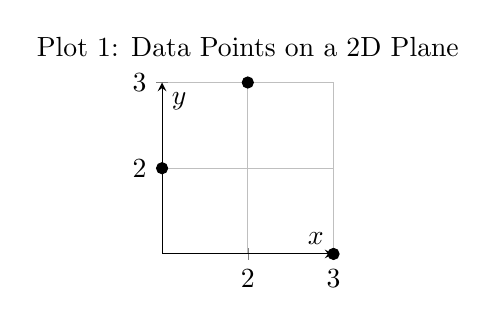
\begin{tikzpicture}
            \begin{axis}[
                title={Plot 1: Data Points on a 2D Plane},
                xlabel={$x$},
                ylabel={$y$},
                axis lines=middle,
                grid=major,
                width=0.31\textwidth,
                height=0.31\textwidth,
                xtick={1, 2, 3},
                ytick={0, 1, 2, 3}
            ]
                \addplot[only marks, mark=*, mark size=2pt] coordinates {(1,2) (2,3) (3,1)};
            \end{axis}
        \end{tikzpicture}
        \hspace{1cm}
        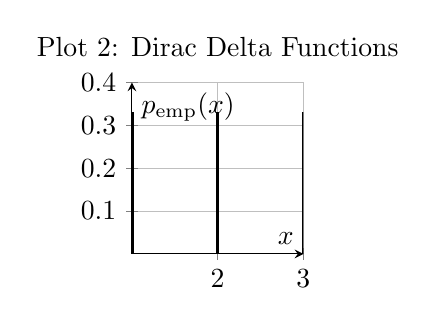
\begin{tikzpicture}
            \begin{axis}[
                title={Plot 2: Dirac Delta Functions},
                xlabel={$x$},
                ylabel={$p_{\text{emp}}(x)$},
                axis lines=middle,
                grid=major,
                width=0.31\textwidth,
                height=0.31\textwidth,
                ymin=0, ymax=0.4,
                xtick={1,2,3},
                ytick={0,0.1,0.2,0.3,0.4}
            ]
                \addplot[very thick] coordinates {(1,0) (1,0.33)};
                \addplot[very thick] coordinates {(2,0) (2,0.33)};
                \addplot[very thick] coordinates {(3,0) (3,0.33)};
            \end{axis}
        \end{tikzpicture}
        \hspace{1cm}
        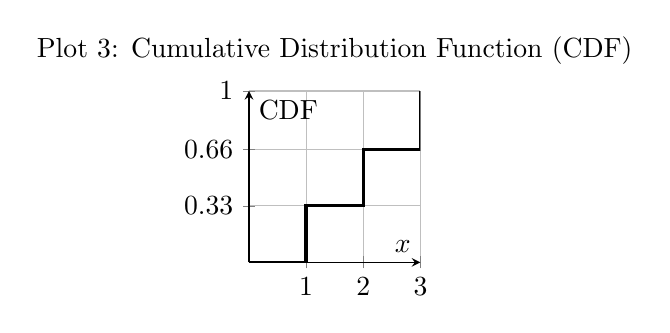
\begin{tikzpicture}
            \begin{axis}[
                title={Plot 3: Cumulative Distribution Function (CDF)},
                xlabel={$x$},
                ylabel={CDF},
                axis lines=middle,
                grid=major,
                width=0.31\textwidth,
                height=0.31\textwidth,
                ymin=0, ymax=1,
                xtick={1, 2, 3},
                ytick={0, 0.33, 0.66, 1}
            ]
                \addplot[very thick] coordinates {(0,0) (1,0) (1,0.33) (2,0.33) (2,0.66) (3,0.66) (3,1)};
            \end{axis}
        \end{tikzpicture}
    \end{center}
    
\end{intuitbox}

\marginnote[-120pt]{    \refsb{Recommended Viewing}{
  \href{https://www.youtube.com/watch?v=7f3YFT7bsmg}{Lecture on Empirical Distribution}\smallskip

  Empirical Statistics: When you compute statistics from a dataset, you're really computing statistics for its empirical distribution.\smallskip

  A dataset is, in essence, a distribution.
}}


\textbf{Empirical Distribution:} Suppose we have a set of data samples 

$$D = \{x^{(1)}, x^{(2)}, \ldots, x^{(N)}\} $$

derived from a random variable \(X\). We can approximate the distribution of \(X\) using a set of delta functions on these samples:
% Represents the distribution of a given data set \(D = \{x^{(1)}, \ldots, x^{(N)}\}\).
\begin{itemize}
    \item For a given data set \(D\), the empirical distribution \(p_{\text{emp}}(x)\) is defined as:
    \[
    p_{\text{emp}}(x) := \frac{1}{N} \sum_{i=1}^N \delta_{x_i}(x)
    \]
    where \(\delta_{x_i}(x)\) is the Dirac measure centred at \(x_i\).
    \item \textbf{Dirac Measure:} \(\delta_{x_i}(x)\) is a function that is 1 if \(x = x_i\) and 0 otherwise. Formally, it is defined as:
    \[
    \delta_{x_i}(x) = \begin{cases} 
    1, & \text{if } x = x_i \\
    0, & \text{if } x \neq x_i 
    \end{cases}
    \]
    \item Explanation: The empirical distribution assigns equal probability \( \frac{1}{N} \) to each observed data point \(x_i\). It is a discrete distribution that places mass only on the observed data points.
    \item In general, one can associate weights with each element of the empirical distribution, i.e., \(p_{\text{emp}}(x) = \frac{1}{N} \sum_{i=1}^N w_i \delta_{x_i}(x)\) as long as each \( 0 \leq w_i \leq 1 \) and \( \sum_{i=1}^N w_i = 1 \).
\end{itemize}

\section{Continuous Random Variables}

\subsection{Gaussian (Normal) Distribution}
\textbf{Probability Density Function (p.d.f):}
\begin{itemize}
    \item Formula: \[
    N(x \mid \mu, \sigma^2) = \frac{1}{\sqrt{2\pi\sigma^2}} \exp\left(-\frac{(x - \mu)^2}{2\sigma^2}\right)
    \]
    \item Mean: \(\mu = \mathbb{E}[X]\).
    \item Variance: \(\sigma^2 = \text{Var}[X]\).
    \item Standard Normal Distribution: \(X \sim N(0, 1)\).
    \item Precision: \(\lambda = \frac{1}{\sigma^2}\).
\end{itemize}
\textbf{Cumulative Distribution Function (CDF):}
\begin{itemize}
    \item Formula: \[
    \Phi(x; \mu, \sigma^2) = \int_{-\infty}^x N(z; \mu, \sigma^2) \, dz
    \]
    \item In terms of the error function (erf):
        \[
        \Phi(x; \mu, \sigma^2) = \frac{1}{2} \left[1 + \text{erf}\left(\frac{z}{\sqrt{2}}\right)\right]
        \]
        where \(z = \frac{x - \mu}{\sigma}\) and
        \[
        \text{erf}(x) = \frac{1}{\sqrt{\pi}} \int_0^x \exp(-t^2) \, dt
        \]
\end{itemize}


\section{Viewing Data}

\begin{itemize}
    \item Data (coordinates) Perspective (Design Matrix) 
    \item Set Perspective
    \begin{itemize}
        \item Combination invariant
        \item Allows for natural language....??
    \end{itemize}
    \item Empirical Distribution Perspective
    \begin{itemize}
        \item i.i.d
    \end{itemize}
\end{itemize}


\section{Example Scene: Self-Driving Car}
\sn{Notation and Gotchas}{
    The lecture use $x_i$ to denote the $i$-th feature, and $x^{(i)}$ to denote the $i$-th data point. The slides however seem to denote $x_i$ as the $i$-th data point. The notes follow the former convention.\\

    Also, it is generally assumed that in a classification problem, the classes are distinct and mutually exclusive, so an image is either a dog or a cat (multi-class classfication) but not a combination of both (multi-label classification). The course focuses on the former convention.

}
Take a case of the self-driving car. There are several facets:
\begin{enumerate}
    \item \textbf{Object Recognition: }identifying objects in the scene (classification)
          \begin{itemize}[noitemsep]
              \item An image is a 2D array of pixel values. For a colour image, each pixel has 3 values (RGB).
              \item \textbf{Input:}
                    \begin{equation}
                        x \in \mathbb{R}^{H \times W \times C}
                    \end{equation}
                    where $H$ is height, $W$ is width, and $C$ is the number of channels (e.g. 3 for RGB)
              \item \textbf{Output:} We would like to detect if something is a background, another vehicle, the ground level, or a pedestrian. Let's say there are $m$ outcomes, making this a \textbf{classification problem}. Naively, let
                    $y \in \mathbb{R}^m$. However, these numbers are just arbitrary i.e. raw scores. It would make more sense to refine the output to a probability distribution over the $m$ classes: \\
                    \begin{equation}
                        y \in \Delta^m \quad \text{where }\sum_{i=1}^{m} y_i = 1
                    \end{equation}
                    Where the $\Delta^m$ is the $m$-simplex, where the sum of all elements is 1. This provides a measure of ``confidence'' in the prediction. Example: To choose between four classes: [Vehicle, Pedestrian, Road, Background], the output could be $[0.1, 0.7, 0.1, 0.1]$. This means the model is 70\% confident that the object is a pedestrian.
              \item \textbf{Our objective is to learn a function:}
                    \begin{equation}
                        f^\theta : x^{(i)} \mapsto y^{(i)} \quad \text{where } \theta \text{ are model parameters}, x^{(i)} \in \mathbb{R}^{H \times W \times C}, y^{(i)} \in \Delta^m
                    \end{equation}
                    \begin{marginfigure}
                        \centering
                        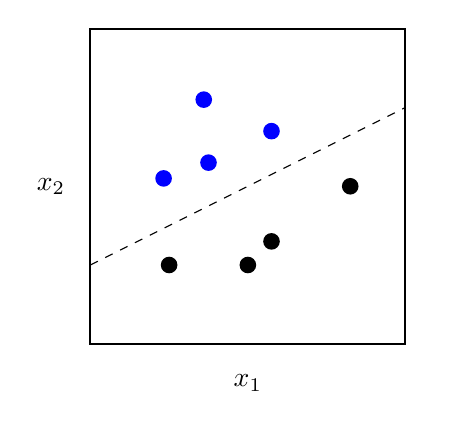
\begin{tikzpicture}
                            % Draw the outer square
                            \draw[thick, black] (0,0) rectangle (4,4);
                            % Draw the blue points
                            \fill[blue] (1.44,3.1) circle (3pt);
                            \fill[blue] (1.5,2.3) circle (3pt);
                            \fill[blue] (0.93,2.1) circle (3pt);
                            \fill[blue] (2.3,2.7) circle (3pt);
                            % Draw the black points
                            \fill[black] (3.3,2) circle (3pt);
                            \fill[black] (2.3,1.3) circle (3pt);
                            \fill[black] (2,1) circle (3pt);
                            \fill[black] (1,1) circle (3pt);
                            % Labels for the axes
                            \node at (2,-0.5) {$x_1$};
                            \node at (-0.5,2) {$x_2$};
                            % Dashed separator
                            \draw[dashed] (0,1)--(4,3) node[right] {};
                        \end{tikzpicture}
                        \caption{Simplified example for $f^\theta$}
                        \label{fig:1_classification}
                    \end{marginfigure}
                    A simplified example for $f^\theta$ is shown in Figure \ref{fig:1_classification}. Ideally, we want a separator that separates the input space into $m$ distinct regions according to observed data.

              \item \textbf{Data Formalisation (1): }We can view our dataset as a set of $N$ pairs where $x^{(i)}$ is an image and $y^{(i)}$ is the corresponding label. More neatly put,
                    \begin{equation}
                        \mathcal{D} = \{(x^{(i)}, y^{(i)})\}_{i=1}^{N}, \quad x^{(i)} \in \mathbb{R}^{H \times W \times C}, y^{(i)} \in \Delta^m
                    \end{equation}
              \item \textbf{Data Formalisation (2): } We could also view the dataset as an empirical distribution over the data space like in Figure \ref{fig:1_distribution}:
                    \begin{equation}
                        \mathcal{D} = \{x^{(i)}, y^{(i)}\}_{i=1}^{N} \sim p_{\text{data}}(x, y)
                    \end{equation}
                    \begin{marginfigure}
                        \centering
                        \begin{tikzpicture}
                            \begin{axis}[
                                view={0}{90},
                                axis on top,
                                enlargelimits=false,
                                colormap/viridis,
                                xlabel={$x_1$},
                                ylabel={$x_2$},
                                % colorbar,
                                samples=50, % Adjusting the sample size
                                domain=-5:5,
                                width=2in,
                                height=2in
                            ]
                            
                            % First contour group
                            \addplot3[
                                contour gnuplot={
                                    levels={0.25, 0.4, 0.55, 0.65, 0.79, 1, 1.25, 1.5}
                                }
                            ]
                            {exp(-((x)^2 + (1.4*y)^2))};
                    
                            % Second contour group
                            \addplot3[
                                contour gnuplot={
                                    levels={0.25, 0.4, 0.55, 0.65, 0.79, 1, 1.25, 1.5}
                                }
                            ]
                            {exp(-((2*x+2)^2 + (y+2)^2))};
                            
                            \end{axis}
                        \end{tikzpicture}
                        \caption{Viewing the dataset as an empirical distribution}
                        \label{fig:1_distribution}
                    \end{marginfigure}
                    



          \end{itemize}
          \item \textbf{Route Planning:} 
          We aim to predict the optimal path, where the prediction function \( f^\theta \) takes spatial data and environmental conditions as input and outputs a route (either as a series of decisions or waypoints).
          \begin{itemize}[noitemsep]
              \item \textbf{Input:}
              \begin{equation}
                  x \in \mathbb{R}^{n}
              \end{equation}
              where \( x \) could represent a vector of features including road conditions, traffic density, and start/end coordinates.
              
              \item \textbf{Output:} 
              A route \( y \), represented either as a classification over a set of discrete routes, or as continuous waypoints:
              \begin{equation}
                  f^\theta : x \mapsto y
              \end{equation}
              Here, \( y \in \mathbb{R}^m \) for \( m \) possible waypoints (or classes, if we use a discrete route classification).
          \end{itemize}
          The objective is to minimise the difference between predicted and actual routes, defined as a suitable loss function \( \mathcal{L}(f^\theta(x), y) \).

    \item \textbf{Speed Control:} 
    \sn{Ordinal Regression here?}{To update}
          In this problem, we predict the optimal driving speed, and \( f^\theta \) models the relationship between environmental and driving conditions and speed.
          \begin{itemize}[noitemsep]
              \item \textbf{Input:} 
              \begin{equation}
                  x \in \mathbb{R}^p
              \end{equation}
              where \( x \) represents features such as current speed, distance to obstacles, road surface, and weather conditions.
              
              \item \textbf{Output:} 
              A continuous speed value \( y \in \mathbb{R} \):
              \begin{equation}
                  f^\theta : x \mapsto y
              \end{equation}
              where \( y \) is the predicted speed. This is a regression problem, so the goal is to minimise the squared error:
              \begin{equation}
                  \mathcal{L}(\theta) = \frac{1}{N} \sum_{i=1}^{N} (f^\theta(x^{(i)}) - y^{(i)})^2
              \end{equation}
          \end{itemize}

    \item \textbf{Steering Angle Prediction:}
          Steering angle prediction aims to output a continuous angle based on the driving conditions, making it a regression problem.
          \begin{itemize}[noitemsep]
              \item \textbf{Input:}
              \begin{equation}
                  x \in \mathbb{R}^q
              \end{equation}
              where \( x \) could represent lane position, vehicle surroundings, and road curvature.
              
              \item \textbf{Output:} 
              The predicted steering angle \( y \in \mathbb{R} \):
              \begin{equation}
                  f^\theta : x \mapsto y
              \end{equation}
              This is also a regression task, and the loss function could again be the squared error:
              \begin{equation}
                  \mathcal{L}(\theta) = \frac{1}{N} \sum_{i=1}^{N} (f^\theta(x^{(i)}) - y^{(i)})^2
              \end{equation}
          \end{itemize}
\end{enumerate}

\section{Mathematics of Linear Models}

Linear models are fundamental in statistics and supervised machine learning. They can:
\begin{itemize}[noitemsep]
    \item Handle linear relationships.
    \item Be augmented with kernels or basis functions to model non-linear relationships.
    \item Provide analytical tractability for studying concepts like convergence, probabilistic modelling, and overfitting.
\end{itemize}
This section introduces the linear regression model.

\subsection{Linear Regression Model}

Linear regression involves performing regression with a linear model in a supervised setting. Given a dataset \(\mathcal{D}\) consisting of input-output pairs \((\bm{x}^{(i)}, y^{(i)})\) for \(i = 1, \ldots, N\):
\begin{itemize}[noitemsep]
    \item \(\bm{x} \in \mathbb{R}^n\) represents the input features.
    \item \(y \in \mathbb{R}\) represents the output or target variable.
    \item Assume a domain \(\mathbb{R}^n\) and a one-dimensional co-domain.
    \item Model: \(f(\bm{x}) = \bm{x}^\top \bm{\theta}\).
    \item Noise: \(\epsilon \sim \mathcal{N}(0, \sigma^2)\).
\end{itemize}
The full model is:
\[
\hat{y}^{(i)} = \bm{x}^{(i)\top} \bm{\theta} + \epsilon
\]

The objective is to find \(\bm{\theta}\) such that \(\hat{y}^{(i)} \approx y^{(i)}\). In other words, we want to find a set of parameters \(\bm{\theta}\) that best explains the relationship between the input features \(\bm{x}\) and the target variable \(y\). This means minimising the difference between the predicted values \(\hat{y}\) and the actual values \(y\).\bigskip

\textbf{Conventions and Notations:}
\begin{itemize}[noitemsep]
    \item Vectors \(\bm{x} \in \mathbb{R}^n\) are column vectors, written as \(n \times 1\) matrices.
    \item \(\bm{x}^\top\) (x transpose) swaps rows and columns of \(\bm{x}\), resulting in a \(1 \times n\) row vector.
\end{itemize}




\begin{referencebox}{Lecture Reading}
    Chapter 1-2 of Kevin Murphy's \textit{Machine Learning: A Probabilistic Perspective}. Chapter 1.4 was not covered, but may be of interest
\end{referencebox}





\chapter{Bond Market}
\section{Introduction}

\begin{definitionbox}{Bond Definition}
    A bond is a certificate issued by a company to raise funds akin to a loan, where it will pay back the principal amount at a specified date, and pay interest at a specified rate.
\end{definitionbox}

Bonds represent a type of security. Like all securities, there must be a legal document that outlines the terms and conditions of the bond. This legal document is called the \textbf{bond indenture}.

\subsection*{Typical Parts of a Bond Indenture}
\begin{itemize}
    \item \textbf{Bond Details}
    \begin{itemize}
        \item Face value or principal amount of the bond
        \item Interest rate, also called the coupon rate payable to bondholders
        \item Maturity date
        \item Any provisions for early redemption or call options
\begin{sidenotebox}{More info on early redemption and call options}
    \begin{itemize}
        \item Callable bonds can be redeemed by the issuer before the maturity date, i.e. the issuer has the right (not obligation) to repay the principal amount before the maturity date.
        \item Puttable bonds can be sold back to the issuer before the maturity date, i.e. the holder of the puttable bond has the right (not obligation) to demand the early repayment of the principal amount.
    \end{itemize}
\end{sidenotebox}
    \end{itemize}
    \item \textbf{Payment Terms}
    \begin{itemize}
        \item Outline the timing and method of interest payments to bondholders
        \item Determines if payments are made periodically (coupon bonds) or as a lump sum at maturity (zero-coupon bonds)
    \end{itemize}
    \item \textbf{Covenants}
    \begin{itemize}
        \item Includes clauses and restrictions to protect bondholders' interests
        \item Example: provisions on issuer's ability to issue more debt
        \item Example: restrictions on the issuer maintaining certain financial ratios
        \item Example: Restricting asset sales or limiting dividend payments
    \end{itemize}
    \item \textbf{Collateral/Security}
    \begin{itemize}
        \item Specifies nature and value of the collateral
        \item Collateral is an asset that the issuer pledges to the bondholders to secure the bond
        \item If the issuer defaults, bondholders can seize the collateral to recover their investment
    \end{itemize}
    \item \textbf{Defaults and Remedies}
    \begin{itemize}
        \item Outlines the conditions under which the issuer is considered in default
        \item Specifies the remedies available to bondholders in case of default
        \item Example: Acceleration clause allows bondholders to demand immediate repayment if the issuer defaults
        \item Example: Appointment of a trustee to represent bondholders' interests, this could mean the trustee can take control of the issuer's assets to repay bondholders
    \end{itemize}
\end{itemize}

\subsection*{Face Value}
The face value of a bond is the notional value or amount that bondholders have lent to the issuer company. The issuer agrees to repay the bondholder this amount at maturity. It is also called the \textbf{par value} or \textbf{principal amount}.

\subsection*{Bond Term}
The term of the bond refers to the duration for which the money has been lent, or the time until the bond reaches maturity.

\subsection*{Payment Terms}
\begin{itemize}
    \item \textbf{Coupon Bonds:} These bonds pay interest to bondholders at regular intervals, typically semi-annually or annually. The interest payment is called the \textbf{coupon payment}. Then at maturity, the bondholder receives the face value of the bond.
    \item \textbf{Zero-Coupon Bonds:} These bonds do not pay interest to bondholders. Instead, they are issued at a discount to the face value, and the bondholder receives a single cash flow equal to the face value at maturity.
\end{itemize}

\begin{definitionbox}{UK Goverment Debt}
    The Debt Management Office (DMO) is responsible for managing the UK government's debt. The DMO issues gilts, which are UK government bonds. Gilts are considered to be risk-free assets, as the UK government is unlikely to default on its debt.
\end{definitionbox}

\section{The Law of One Price}
The law of one price states that identical goods should sell for the same price in different markets. This principle applies to bonds, where two bonds with the same risk and cash flows should sell for the same price.


\subsection*{Government Debt (Sovereign Bonds)}
\begin{itemize}
    \item It is generally assumed that governments honour their debt obligations, so government bonds are considered risk-free.
    \item This simplifies the valuation of government bonds, as we assume that we can exclude considerations of credit risk, the possibility of default.
    \item \textbf{Zero-Coupon Bonds} are the simplest type, often called zeros. They are sold at a discount to the face value, and the bondholder receives the face value at maturity. There are no coupon payments.
    \begin{itemize}
        \item It is simple to calculate the price of a zero-coupon bond, as there are only two cash flows: the purchase price and the face value.
        \item The investor pays a price $P$ for the bond to the government.
        \item The government pays the face value $FV$ to the investor at maturity
        \item Since the initial price $P$ is discounted from $FV$, we define the interest rate, or yield to maturity, $r$ as the rate that equates the present value of the face value to the price paid, over $N$ periods.
        \item The yield to maturity represents the average return over the bond's term for the investor.
        \item We have the formulas:
        \begin{equation}
               P = \frac{FV}{(1 + r)^N}
              \end{equation}
        \begin{equation}
                r = \left(\frac{FV}{P}\right)^{\frac{1}{N}} - 1
        \end{equation}
    \end{itemize}
    \item \textbf{Coupon Bonds} involve regular coupon payments to bondholders, in addition to the face value at maturity. A coupon payment is referred to as $C$. 
    \begin{equation}
        C = \frac{\text{Coupon Rate} \times FV}{\text{Number of interest payments per year}}
    \end{equation}
    \item The price of a coupon bond is the sum of the present value of the coupon payments and the present value of the face value, where $N$ is the number of periods until maturity. 
        \begin{align}
            P &= \sum_{t=1}^{N} \frac{C}{(1 + r)^t} + \frac{FV}{(1 + r)^N}\\
              &\equiv C \times \frac{ 1-(1+ r)^{-N}}{r} + \frac{FV}{(1 + r)^N}
          \end{align}
    \item In the second line, the geometric sum formula is used to simplify the sum of the coupon payments.
    \item It is easy to see that the current price of a bond is inversely related to the yield to maturity. If the yield to maturity increases, the bond price decreases, and vice versa.
    \item This is because when yield to maturity increases, fewer people want to buy a bond with a coupon rate that is relatively lower than the yield to maturity (they will prefer a bond with a higher coupon rate to offset the increased yield to maturity).
    \item Another attribute of a bond is its current yield, which is the annual coupon payment divided by the bond's price.
    \begin{equation}
        \text{Current Yield} = \frac{\text{Annual Rate}}{P} = \frac{\text{Coupon Rate} \times FV}{P}
    \end{equation}
        
\end{itemize}

\subsection*{Examples of the Law of One Price}
\subsubsection*{Bonds vs Deposit}
\begin{itemize}
    \item Assume interest rates are constant, and are expected to remain so at say, 5\%.
    \item Consider a coupon-paying bond with coupons equal to 5\% of the face value.
    \item The bond would be selling at par, meaning its price equals its face value.
    \item The coupon payments are then directly equivalent to interest payments, and the final redemption payment is the face value.
    \item Investing in the bond would provide the same return as a deposit account paying 5\% interest, with the same cash flows.
    \item Therefore, the bond's price and the deposit account's value should be the same due to the law of one price.
\end{itemize}

\subsubsection*{Two Government Bonds}
\begin{itemize}
    \item Consider a French bond and a German bond, both denominated in Euros.
    \item In a well-functioning market, we would assumedly expect the returns from lending to the French government to be approximately the same as lending to the German government.
    \item Therefore, we would not expect a significant difference in yield to maturity on the average interest rate paid by each government.
    \item If there was a large disparity in returns under normal market conditions, investors would prefer the bond offering the higher return.
    \item This would lead to increased demand for that bond, causing its price to rise and its yield to decrease until it reaches a level equal to the other bond.
    \item In an efficient market, comparable bonds with similar risk profiles would have equal yields to maturity, which can be seen as the market interest rate for that bond's term. 
    \item Consequently, we can refer to the yield to maturity of a two-year zero as the interest rate on two-year money, without distinguishing the specific instrument, as an efficient market would have similar rates across different types of bonds.
\end{itemize}

\begin{examplebox}{Coupon Bond Calculation Questions}
\textbf{Question 1:} A bond has a 7\% coupon and pays interest semi-annually. What is the amount of each interest payment if the face value of a bond is \pounds100?

\textbf{Answer:}
The interest payment, or coupon payment, for a bond can be calculated using the formula:
\[ \text{Interest payment} = \frac{\text{Coupon rate} \times \text{Face amount}}{\text{Number of interest payments per year}} \]

For a 7\% coupon rate with semi-annual payments:
\[ = \frac{0.07 \times \pounds100}{2} \]
\[ = \frac{\pounds7}{2} \]
\[ = \pounds3.50 \]

\textbf{Question 2:} A bond has a 9\% coupon rate, matures in three years, and pays interest semi-annually. The face value is \pounds100. What is the current price of this bond if the market rate of return is 8.3\%?

\textbf{Answer:}
The current price of the bond can be calculated using the present value of future cash flows. The formula for the bond price using the longhand method is:
\[ P = \frac{C}{(1+r)} + \frac{C}{(1+r)^2} + \cdots + \frac{C + FV}{(1+r)^t} \]

Where \( C \) is the coupon payment, \( FV \) is the face value, \( r \) is the market rate of return per period, and \( t \) is the total number of periods.

Given a 9\% coupon rate, with semi-annual payments and a market rate of return of 8.3\%, the bond price is:
\begin{align*} P &= \frac{\pounds4.5}{(1.0415)}  +  \frac{\pounds4.5}{(1.0415)^2} + \cdots + \frac{\pounds104.5}{(1.0415)^6} \\
&=\left(\frac{0.09\times£100}{2}\times\frac{1-\left[\frac{1}{\left(1+\frac{0.083}{2}\right)^{3\times2}}\right]}{\frac{0.083}{2}}\right)+\frac{£100}{\left(1+\frac{0.083}{2}\right)^{3\times2}}
\end{align*}
\[ = \pounds101.83 \]

The shorthand method for the bond price is:
\[ P = \left( CPN \times \left[ \frac{1 - \left[ \frac{1}{(1+r)^t} \right]}{r} \right] \right) + \frac{FV}{(1+r)^t} \]
\[ = \pounds101.83 \]

\textbf{Question 3:} An 8\%, semi-annual coupon bond has a \$1000 face value and matures in eight years. What is the current yield on this bond if the yield to maturity is 7.8\%?

\textbf{Answer:}
The current yield is calculated as:
\[ \text{Current yield} = \frac{\text{Annual yield}}{\text{Current price}} \]

We first calculate the current price:

\begin{align*}
    P&=\left(CPN\times\left(\frac{1-\left[\frac1{\left(1+r\right)^{t}}\right]}{r}\right)\right)+\frac{FV}{\left(1+r\right)^{t}} \\
    P&=\left(\frac{0.08\times1000}{2}\times\left(\frac{1-\left[\frac{1}{(1+\frac{0.078}{2})^{8\times2}}\right]}{\frac{0.078}{2}}\right)\right)+\frac{1000}{\left(1+\frac{0.078}{2}\right)^{8\times2}} \\
    &=(\$40\times11.73873)+\$542.18967 \\
    &=\$469.54920+\$542.18967 \\
    &=\$1,011.74
\end{align*}

For an 8\% coupon rate with a \$1000 face value and a yield to maturity of 7.8\%:
\[ = \frac{\$80}{\$1011.74} \]
\[ = 0.07907 \]
\[ = 7.91\% \]
\end{examplebox}

\renewcommand{\thesection}{2.3 - 2.4}
\section{Yield Curves}
\setcounter{section}{4}
\renewcommand{\thesection}{\arabic{chapter}.\arabic{section}}

A yield curve is a representation of how the market expects interest rates to vary in the future.

It shows the relationship between the yield to maturity and the time to maturity for a set of similar bonds. The following diagram shows a typical yield curve for zero-coupon bonds.

\begin{figure}[H]
    \centering
    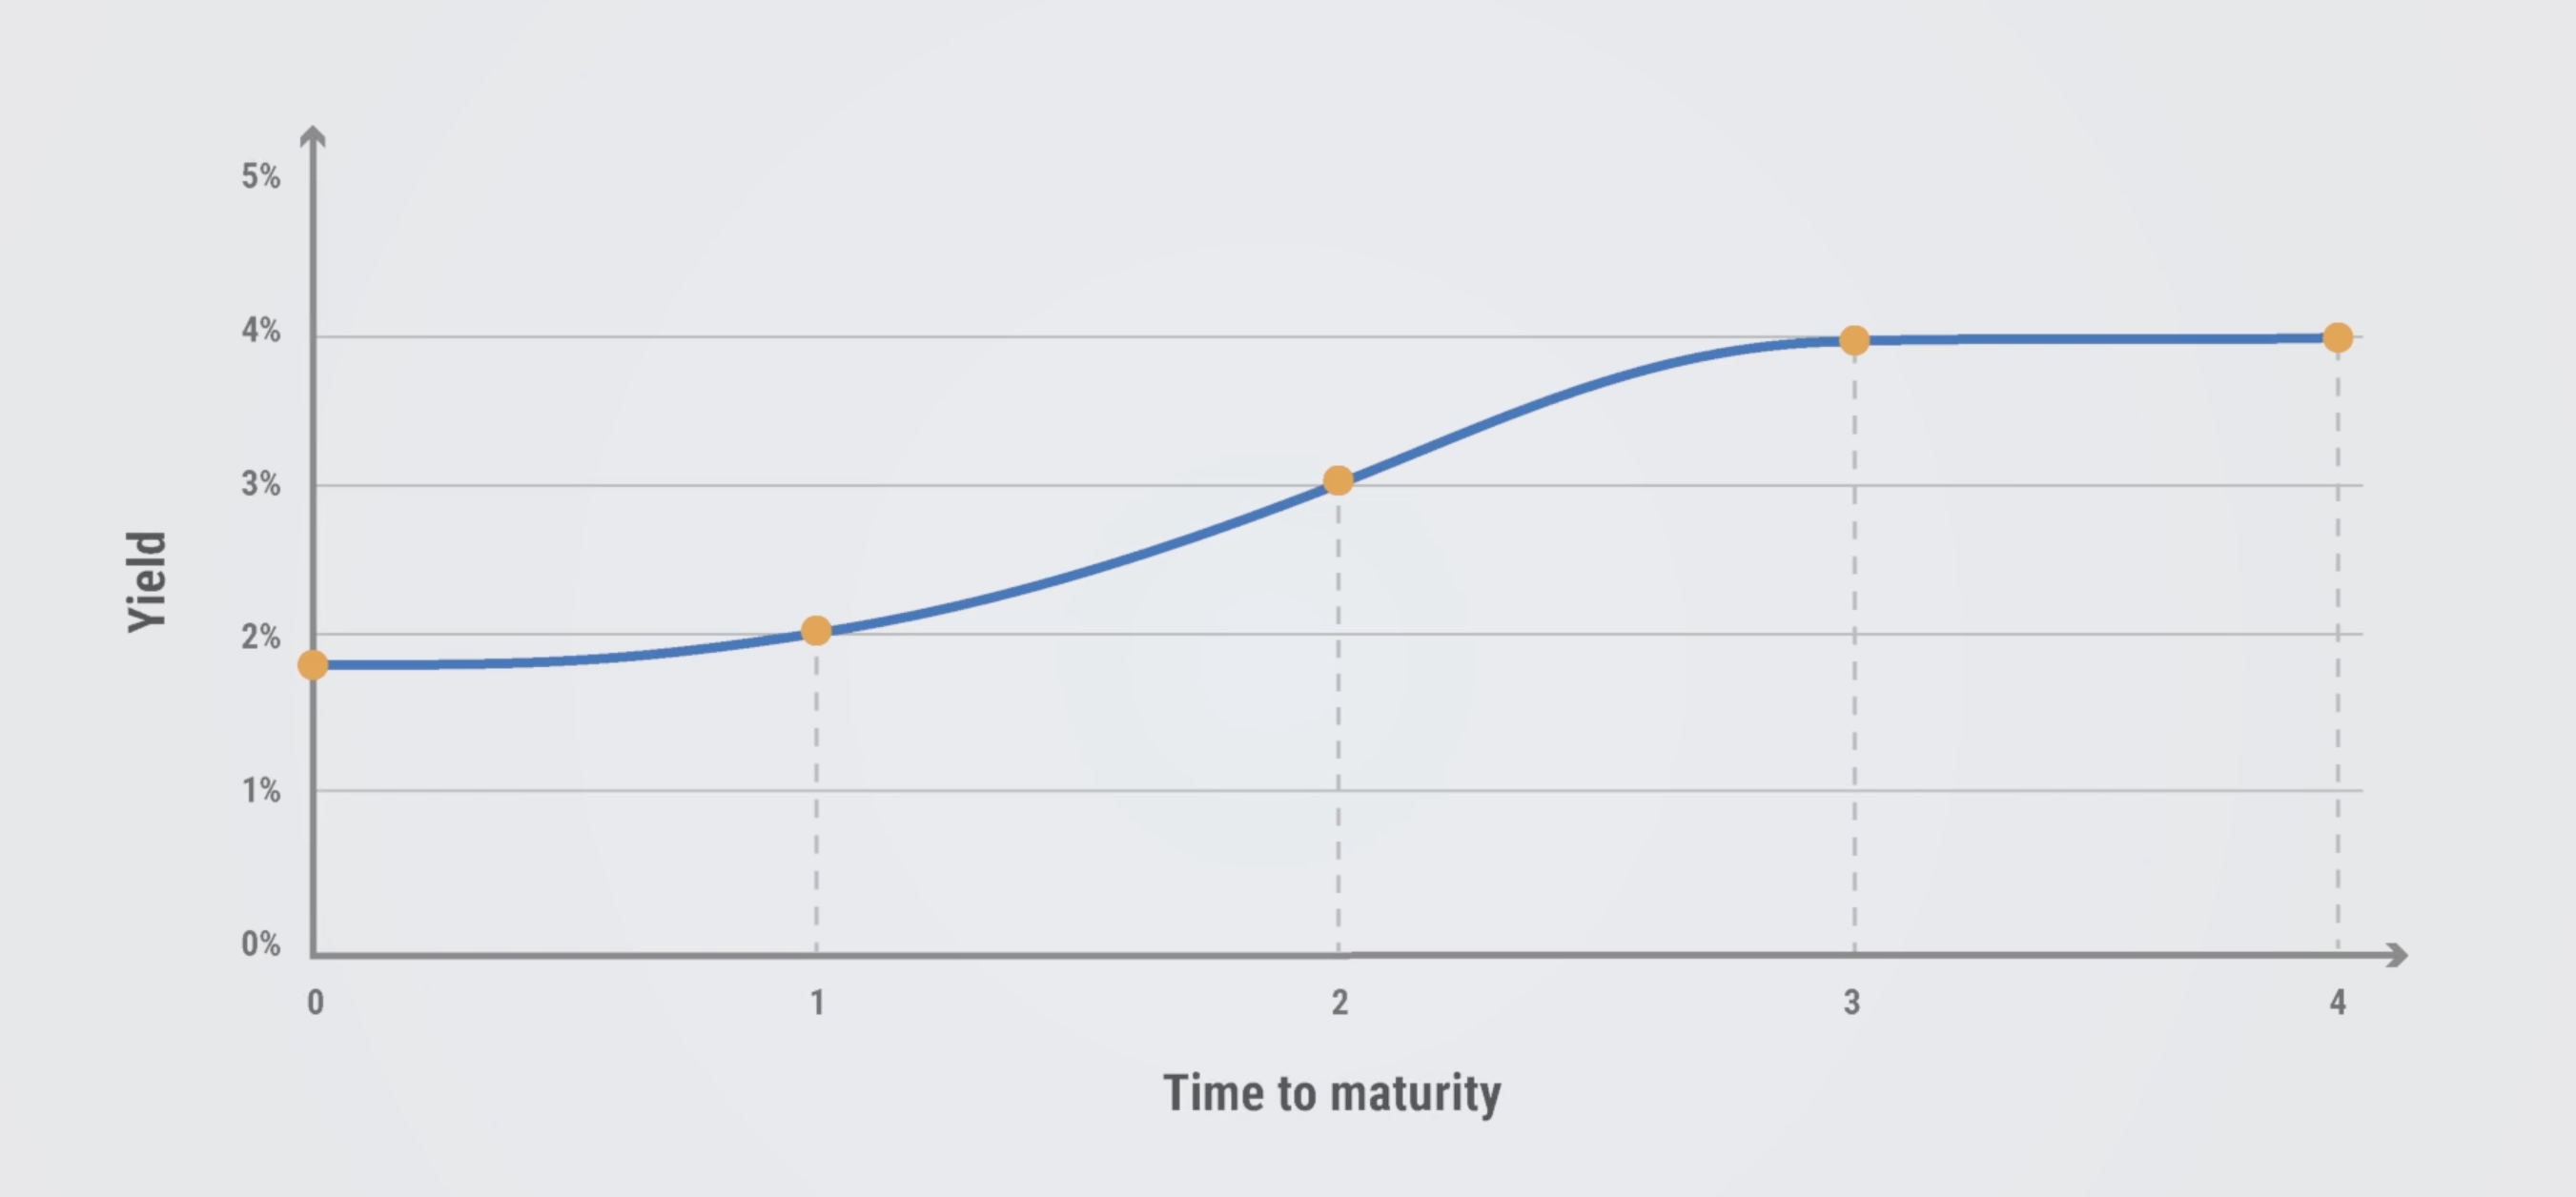
\includegraphics[width=0.8\textwidth]{img/2.1.png}
    \caption{Yield Curve for Zero-Coupon Bonds}
    \label{fig:yield_curve}
\end{figure}

The yield for a one-year zero-coupon bond is 2\%, for a two-year bond it is 3\%, and for a three-year bond it is 4\%. This is an example of a normal yield curve, where longer-term bonds have higher yields than shorter-term bonds. \\


There is a gradual increase in interest rates as the time to maturity increases, but this does not always hold. In this case, the increase tapers off at 5\%, for a four-year bond. This is known as the \textbf{flattening} of the yield curve, and that the markets expect interest rates to remain stable in the long term.

\section{Pricing Coupon Bonds with the Yield Curve}

It is trivial to price coupon bonds with a variable rate determined by the yield curve. 

Using the example yield curve in Figure \ref{fig:yield_curve}, and assuming round numbers for simplicity, we have:

\begin{table}[htbp]
    \centering
    \caption{Yield Curve for Zero-Coupon Bonds}
    \label{tab:yield_curve}
    \begin{tabular}{@{} c c c @{}}
    \toprule
    \textbf{Time to Maturity} & \textbf{Yield to Maturity} & \textbf{Discounted Payment} \\
    \midrule
    1 year & 2\% & ${5}/{(1+0.02)^1}$\\
    2 years & 3\% & ${5}/{(1+0.03)^2}$\\
    3 years & 4\% & ${5}/{(1+0.04)^3}$\\
    4 years & 4\% & ${(5+100)}/{(1+0.04)^4}$\\  
    \bottomrule
    \end{tabular}
\end{table}

Where the last payment includes the face value of the bond.\\

To price a four-year coupon bond with a 5\% coupon rate for the face value of £100 with annual payments, this will be a £5 coupon payment in years 1-3, followed by a £105 payment in year 4.\\

We thus have the following for the fair price of the bond:

\[
P = \frac{5}{(1+0.02)^1} + \frac{5}{(1+0.03)^2} + \frac{5}{(1+0.04)^3} + \frac{105}{(1+0.04)^4}  = 103.8
\]
\renewcommand{\thesection}{2.6 - 2.8}
\section{Yield Curve (Live Class)}
\setcounter{section}{8}
\renewcommand{\thesection}{\arabic{chapter}.\arabic{section}}

\subsection*{The Company's Balance Sheet}

\begin{figure}[H]
    \centering
    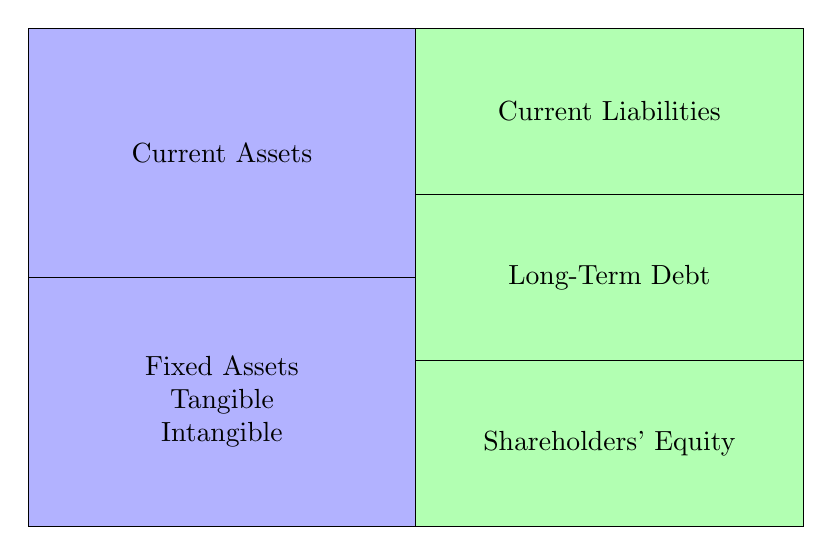
\begin{tikzpicture}
        % Define the styles for each block
        \tikzstyle{block} = [rectangle, draw, fill=blue!30, text width=14em, text centered, minimum height=9em, inner sep=0, outer sep = 0]
        \tikzstyle{blockgreen} = [rectangle, draw, fill=green!30, text width=14em, text centered, minimum height=6em, inner sep=0, outer sep = 0]

        % Define the nodes for Current Assets and Fixed Assets
        \node[block] (current) {Current Assets};
        \node[block, below=0 of current] (fixed) {Fixed Assets\\Tangible\\Intangible};

        % Calculate the total height of the left blocks (current and fixed)
        \path let \p1 = ($(current.north)-(fixed.south)$), \n1 = {veclen(\y1,\x1)} in -- (current.north east) coordinate (middlepoint);

        % Define the nodes for Current Liabilities, Long-Term Debt, and Shareholders' Equity
        % Adjust the heights to account for the borders of the nodes
        \node[blockgreen, below=0 of middlepoint, anchor=north west, ] (currentliab) {Current Liabilities};
        \node[blockgreen, below=0 of currentliab.south west, anchor=north west, ] (longterm) {Long-Term Debt};
        \node[blockgreen, below=0 of longterm.south west, anchor=north west, ] (equity) {Shareholders' Equity};
    
    \end{tikzpicture}
    \caption{Simplified diagram graphic of the Company Balance Sheet.}
    \label{fig:balance_sheet}
\end{figure}

The table in Figure \ref{fig:balance_sheet} shows a simplified version of a company's balance sheet. Current assets could refer to cash, inventory, or accounts receivable. Fixed assets could refer to property, manufacturing plants, and equipments. Current liabilities could refer to accounts payable, short-term loans, or taxes payable. Long-term debt could refer to bonds or loans with a maturity of more than one year. 

Figure \ref{fig:balance_sheet} also shows the fundamental accounting equation: 
\begin{equation}
    \text{Assets} = \text{Liabilities} + \text{Equity}
\end{equation}

Which is rewritten as:
\begin{equation}
    \text{Equity} = \text{Assets} - \text{Liabilities}
\end{equation}

This simply means that shareholders own all of the assets minus liabilities, i.e. the company's equity is the residual value of the company's assets after all liabilities have been paid off.\\

\subsection*{Capital Budgeting Decision}

We take the previous table from Figure \ref{fig:balance_sheet} and simplify it further:

\begin{figure}[H]
    \centering
    \begin{tikzpicture}
        % Define the styles for blocks and labels
        \tikzstyle{block} = [rectangle, draw, fill=blue!30, text width=14em, text centered, minimum height=9em, inner sep=0, outer sep = 0]
        \tikzstyle{block2} = [rectangle, draw, fill=blue!30, text width=14em, text centered, minimum height=3em, inner sep=0, outer sep = 0]
        \tikzstyle{blockgreen} = [rectangle, draw, fill=green!30, text width=14em, text centered, minimum height=6em, inner sep=0, outer sep = 0]
        \tikzstyle{labelstyle} = [rectangle, text width=14em, text centered, inner sep=0, outer sep = 0]

        % Labels for the columns
        \node[labelstyle] (label1) at (0em,0em) {Invested Capital};
        \node[labelstyle] (label2) at (14em,0em) {Equity and Debt};
        

    
        \path let \p1 = (label1.south), \p2 = (current.north) in [yshift=(\y1-\y2)] node[labelstyle] at (current.north) {};

        % Define the nodes for Current Assets and Fixed Assets
        \node[block2, below=of label1] (current) {Net Working Capital = C. Assets $-$ C. Liabilities};
        \node[block, below=0 of current] (fixed) {Fixed Assets\\Tangible\\Intangible};

        % Calculate the total height of the left blocks (current and fixed)
        \path let \p1 = ($(current.north)-(fixed.south)$), \n1 = {veclen(\y1,\x1)} in -- (current.north east) coordinate (middlepoint);

        % Define the nodes for Long-Term Debt, and Shareholders' Equity
        \node[blockgreen, below=of label2] (longterm) {Long-Term Debt};
        \node[blockgreen, below=0 of longterm] (equity) {Shareholders' Equity};


    \end{tikzpicture}
    \caption{Processed diagram graphic of the Company Balance Sheet.}
    \label{fig:balance_sheet_2}
\end{figure}


This operation now defines the left column as invested capital. It is used to ask what long-term investments that the firm should choose to maximise value. The right column is equity and debt, which is used to ask how the firm should finance these investments.\\

The value of the firm can be thought of as a pie:

\begin{figure}[H]
    \centering
    \begin{subfigure}{0.4\textwidth}
        \centering
        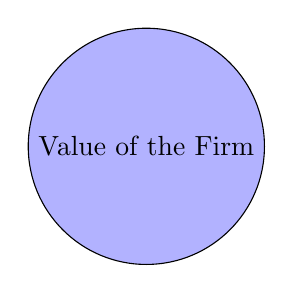
\begin{tikzpicture}
            \draw[fill=blue!30] (0,0) circle (1.5cm) node[midway] {Value of the Firm};
        \end{tikzpicture}
        \caption{Value Composition}
        \label{fig:value_firm1}
    \end{subfigure}
    \begin{subfigure}{0.4\textwidth}
        \centering
        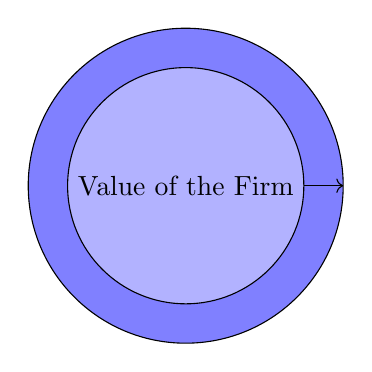
\begin{tikzpicture}
            \draw[fill=blue!50] (0,0) circle (2cm) node[midway] {};
            \draw[fill=blue!30] (0,0) circle (1.5cm) node[midway] {Value of the Firm};
            \draw[fill=black, ->] (1.5cm,0) -- (2.0,0cm) node[midway, yshift=0.5cm] {};
        \end{tikzpicture}
        \caption{Value Composition Increased}
        \label{fig:value_firm2}
    \end{subfigure}
    \caption{Goal: increase pie size }
    \label{fig:value_firm}
\end{figure}

The role of the manager is to increase the size of the pie's net present value. The Capital Structure decision can be viewed as how best to slice the pie.

\begin{figure}[H]
    \centering
    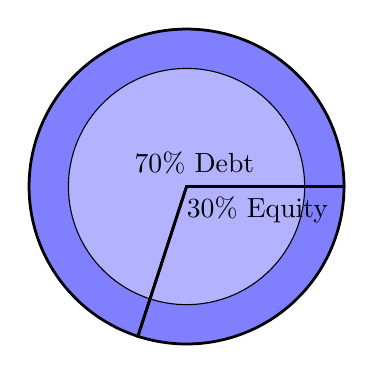
\begin{tikzpicture}
        % Draw the filled circles
        \draw[fill=blue!50] (0,0) circle (2cm); % Outer circle
        \draw[fill=blue!30] (0,0) circle (1.5cm) node[midway] {}; % Inner circle

        % Add the arcs for the pie chart on top
        % Outline of 70% Debt arc
        \draw[line width=1pt] (0,0) -- (2cm,0) arc (0:252:2cm) -- cycle;
        % Outline of 30% Equity arc
        \draw[line width=1pt] (0,0) -- (2cm,0) arc (0:-108:2cm) -- cycle;
        
        % Labels for Debt and Equity
        \node at (0.1cm,0.3cm) {70\% Debt};
        \node at (0.9cm,-0.3cm) {30\% Equity};
    \end{tikzpicture}
    \caption{The capital structure decision slices the pie.}
    \label{fig:debt_equity_circle}
\end{figure}

\subsection*{The Role of Financial Markets}

\begin{figure}[H]
    \centering
    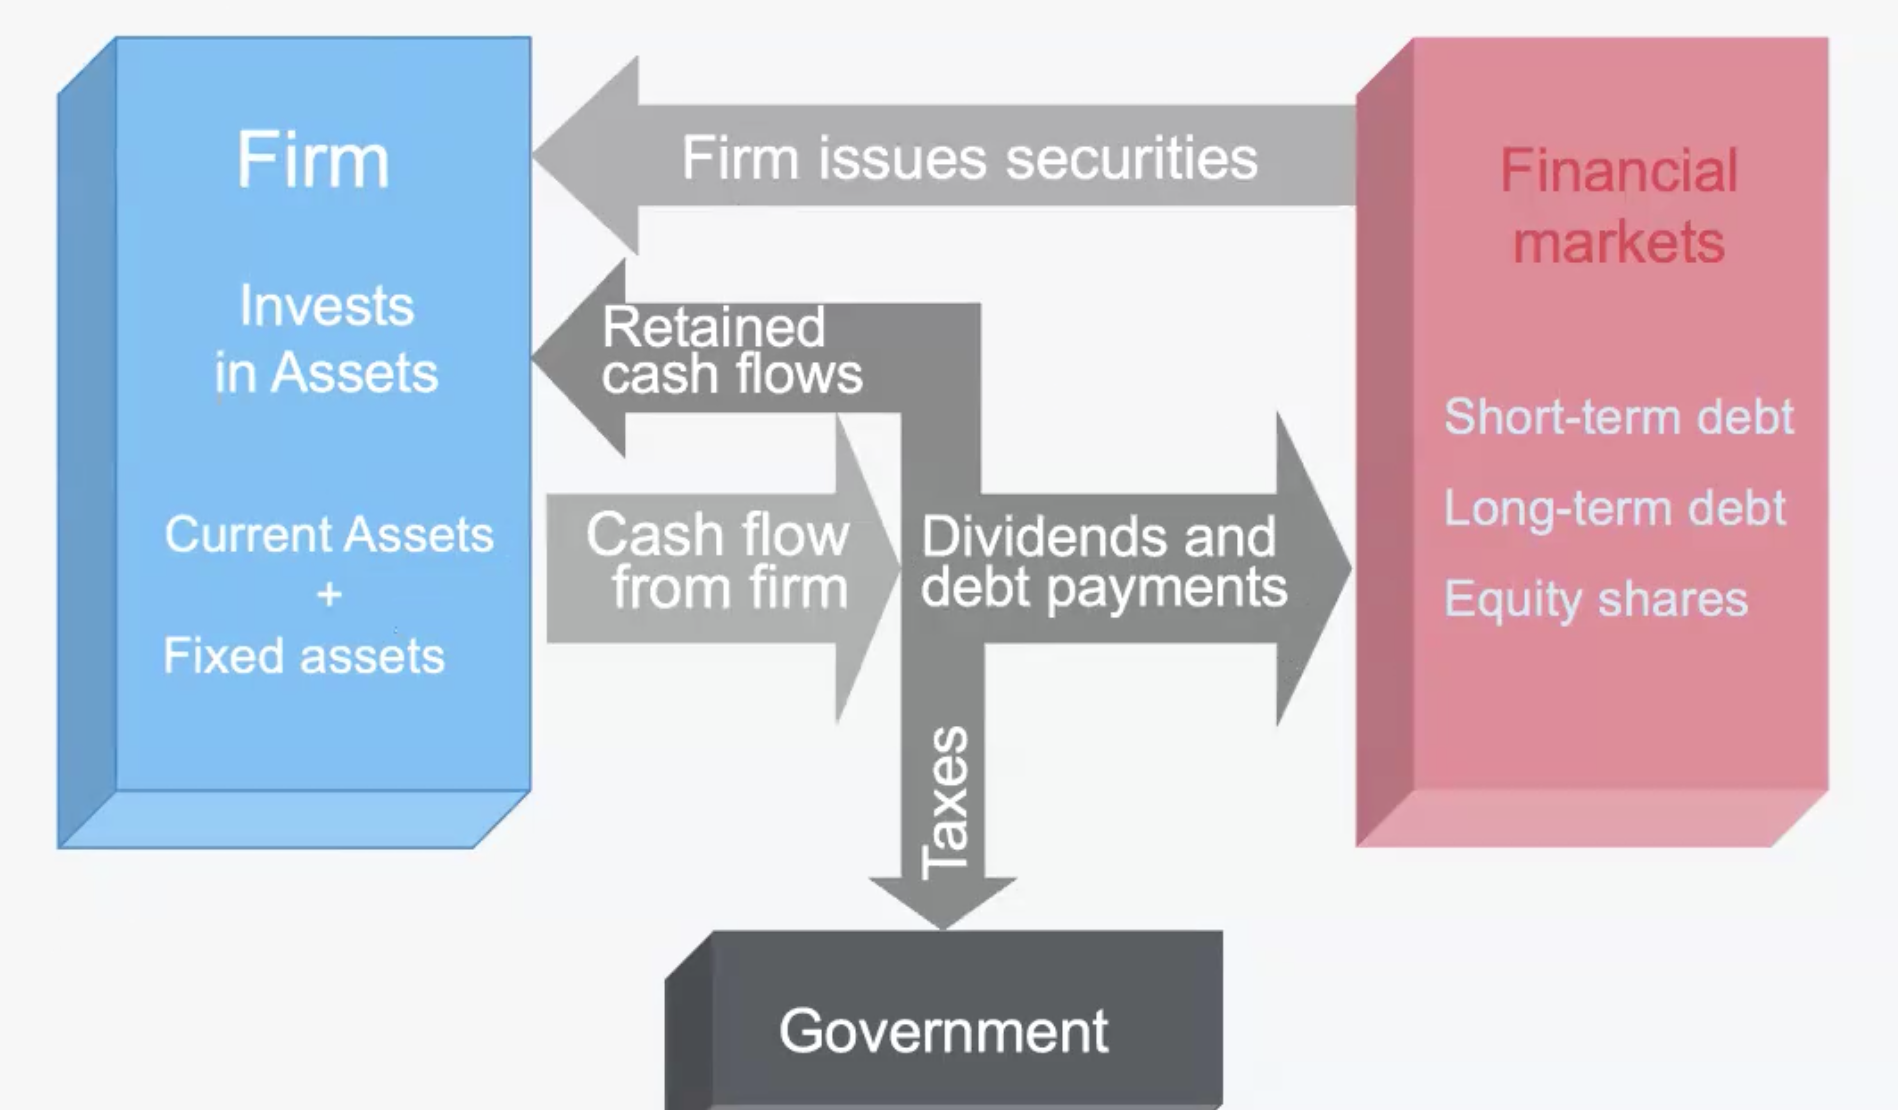
\includegraphics[width=0.8\textwidth]{img/2.2.png}
    \caption{The Role of Financial Markets}
\end{figure}

\begin{itemize}
    \item Company raises money to invest in assets through equity or debt.
    \item Equity or debt gets traded in the market.
    \item Company compensates investors with dividends or interest
    \item Company pays taxes to government
\end{itemize}

\subsection*{Yield Curves}
\begin{itemize}
    \item Term structure of interest rates, or the yield curve, is how zero-coupon bond yields change with bond maturity.
    \item When pricing bonds, we often assume a flat yield curve for simplicity. 
    \item This is not always the case, as they are generally upward sloping (but not always).
    \item Yield curve is usually represented by spot rates. A spot rate is the rate of interest on a bond with a single cash flow at a specific future date.
\end{itemize}

\begin{figure}[H]
    \centering
    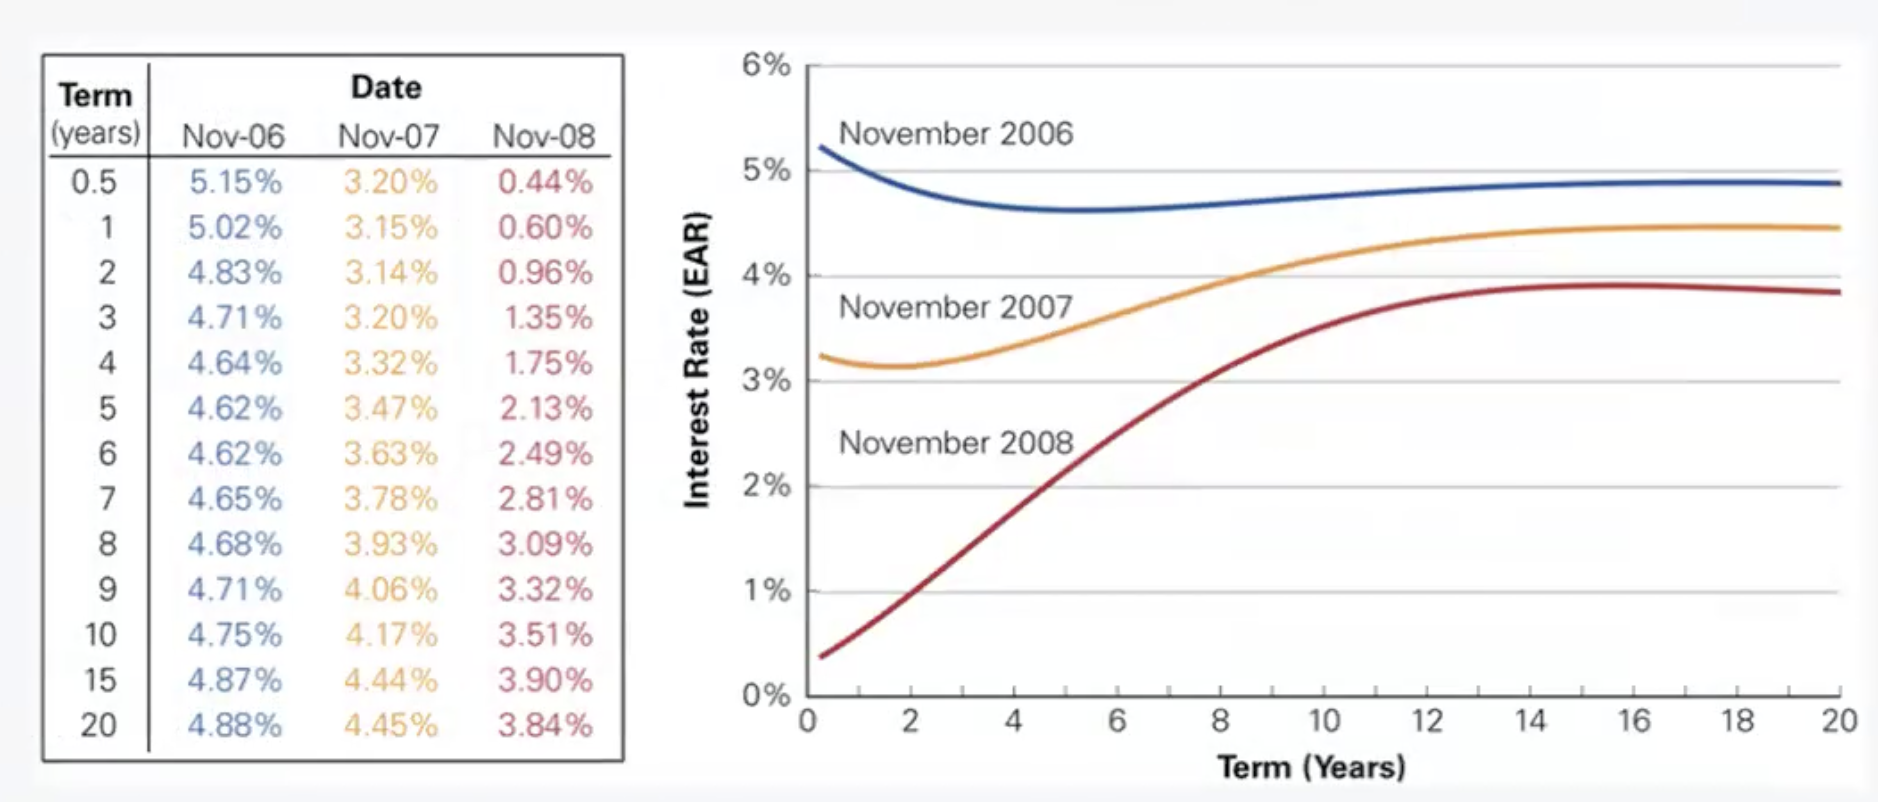
\includegraphics[width=0.8\textwidth]{img/2.3.png}
    \caption{Term Structure of Risk-Free U.S. Interest Rates, Nov 2006, 2007, 2008}
    \label{fig:term_structure}
\end{figure}
\begin{figure}[H]
    \centering
    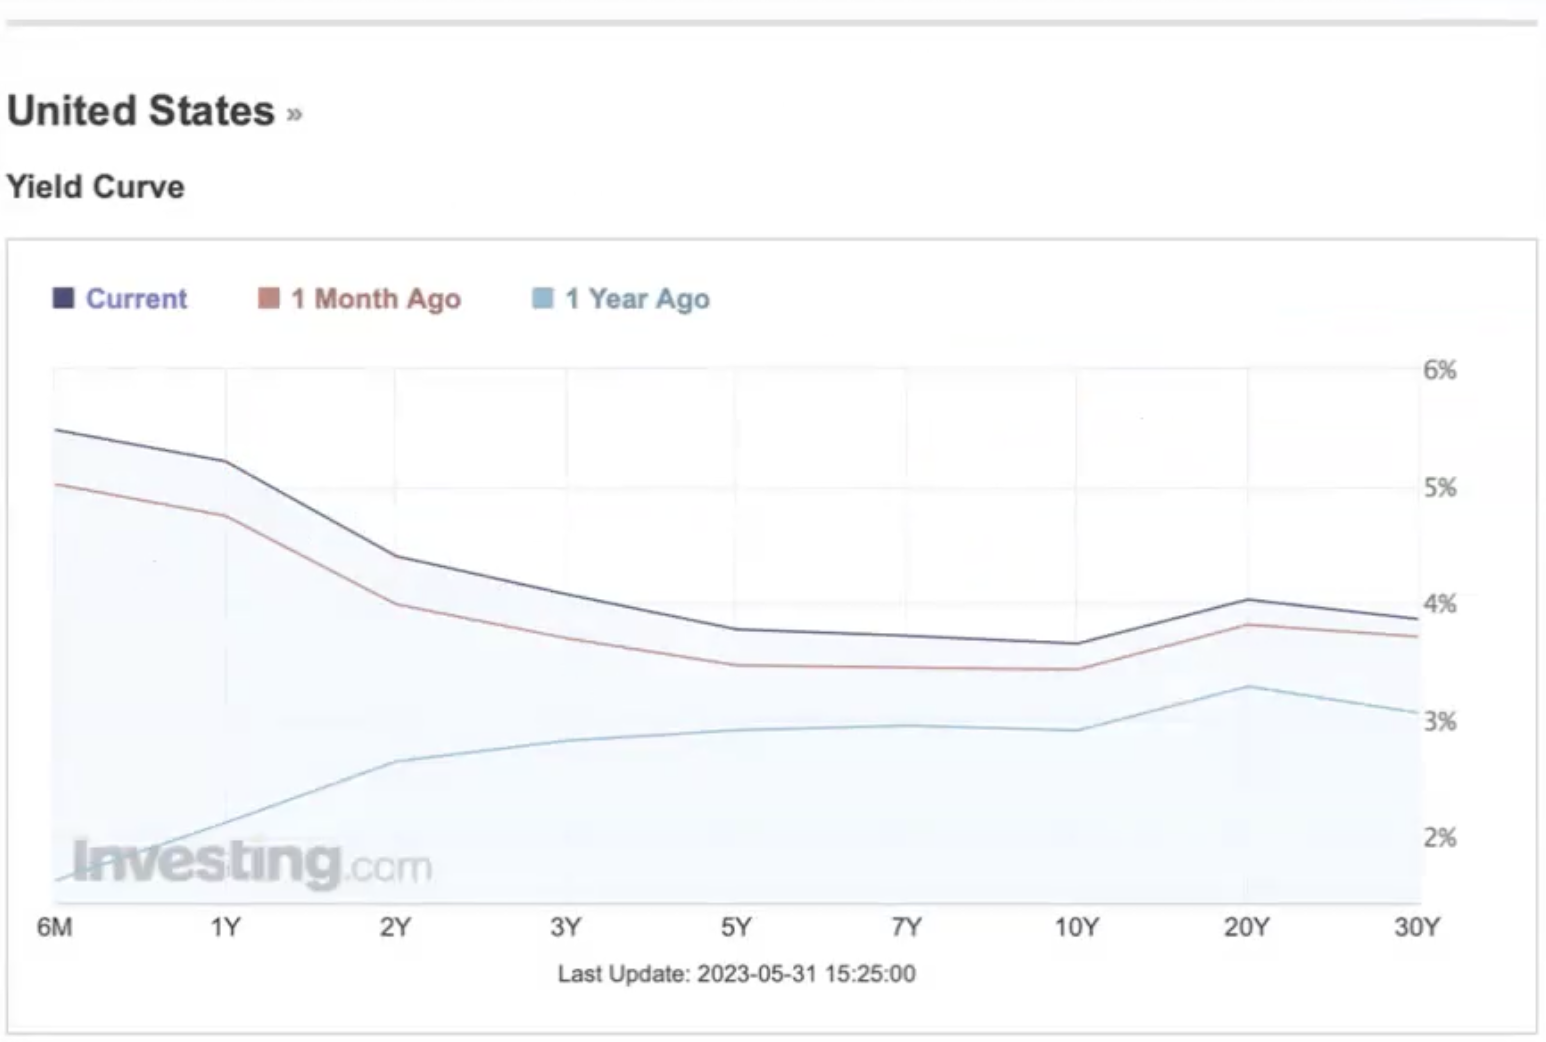
\includegraphics[width=0.8\textwidth]{img/2.4.png}
    \caption{Term Structure of Risk-Free U.S. Interest Rates, May 2023}
    \label{fig:term_structure2}
\end{figure}

From Figure \ref{fig:term_structure}, it can be seen that in November 2006 prior to the 2008 financial crisis, the yield curve was had relatively higher interest rates for the first two years, indicating an inverted yield curve which is a sign of an impending recession.\\

Similarly, in Figure \ref{fig:term_structure2}, the economy had an inverted yield curve in May 2023, despite a year ago having an upward sloping yield curve. 

\subsubsection*{Inverted Yield Curve as a sign of Recession} 
\begin{itemize}
    \item Normally, longer-term debt instruments should have a higher yield than shorter-term ones due to the increased risk of holding the bond for a longer period from inflation and the uncertainty of future interest rates.
    \item An inverted yield curve is when short-term debt instruments have a higher yield than longer-term ones. This is because investors expect future economic growth to slow, and that the central bank will have to lower interest rates to stimulate the economy.
    \item They are therefore then willing to accept lower yields on long-term bonds now, on the expectation that returns on future investments will be similarly low, if not lower. A long-term bond is generally a safer investment in times of economic uncertainty. 
    \item An inverted yield curve reduces the profitability of banks, as they borrow short-term and lend long-term, so the \textit{spread} between what banks can earn on long-term loans and what they pay on short-term borrowings decreases. This causes the bank to be more cautious in providing loans, leading to a reduction in lending, which can slow down the economy. 
    \item Furthermore, consumers expect interest rates to drop in the future (a common reason behind the inverted yield curve), and will postpone borrowing, also decreasing demand for loans in the short-term in banks. Conversely, if banks anticipate lower future interest rates, they will be less willing to offer long-term loans at current rates.
    \item Historically, an inverted yield curve has been a reliable indicator of an impending recession.
\end{itemize}

\subsection*{Spot Rates to Build Yield Curves}
Yield curves are built from spot rates, which are known today and start today. They are determined from yield to maturities on discount(zero-coupon) bonds, annualised for comparison purposes.\\

E.g. if I want to get a mortgage or a deposit, I check the spot rate for the term I want to borrow or lend for.\\

\begin{figure}[H]
    \centering
    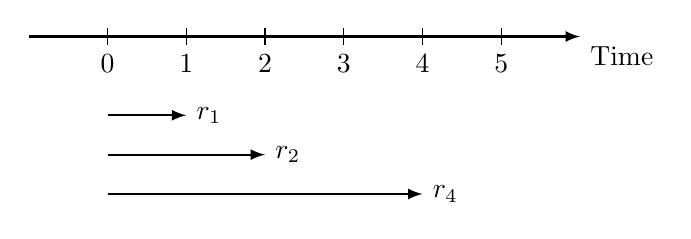
\begin{tikzpicture}
        % Draw the main number line
        \draw[thick, -latex] (-1,0) -- (6,0) node[anchor=north west] {Time};
        
        % Draw the spokes for 0-5
        \foreach \x in {0,...,5} {
          \draw (\x cm,3pt) -- (\x cm,-3pt) node[anchor=north] {$\x$};
        }
        
        % Draw the arrows for r1, r2, and r4
        \draw[thick, -latex] (0,-1) -- (1,-1) node[right, fill=white] {$r_1$};
        \draw[thick, -latex] (0,-1.5) -- (2,-1.5) node[right, fill=white] {$r_2$};
        \draw[thick, -latex] (0,-2.0) -- (4,-2.0) node[right, fill=white] {$r_4$};
    \end{tikzpicture}
    
\end{figure}

$r_1$ is the interest rate from time 0 to time 1, $r_2$ is the interest rate from time 0 to time 2, and so on.\\

\begin{examplebox}{Spot Rate Example Calculations}

\textbf{Question:} Suppose that a 5-year pure discount bond with face value \$100 is selling for \$95, what is the YTM on this bond?

\begin{align*}
    95 = \frac{100}{(1 + r_5)^5} \\
    (1+r_5)^5 = \frac{100}{95} \\
    r_5 = \left(\frac{100}{95}\right)^{\frac{1}{5}} - 1 = 1.031\%
\end{align*}

\end{examplebox}

\subsection*{Forward Rates}

The Bank of England website actually shows forward rates as default rather than spot rates. This is because the forward rate is the rate that you can lock in today as a loan or deposit for a future period.\\

\begin{itemize}
    \item Forward rates are interest rates set today for a future loan
    \item These rates are known today, but\textbf{ start in the future}
\end{itemize}


\begin{figure}[H]
    \centering
    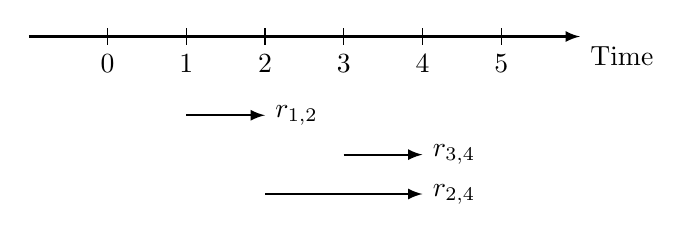
\begin{tikzpicture}
        % Draw the main number line
        \draw[thick, -latex] (-1,0) -- (6,0) node[anchor=north west] {Time};
        
        % Draw the spokes for 0-5
        \foreach \x in {0,...,5} {
          \draw (\x cm,3pt) -- (\x cm,-3pt) node[anchor=north] {$\x$};
        }
        
        % Draw the arrows for r1, r2, and r4
        \draw[thick, -latex] (1,-1) -- (2,-1) node[right, fill=white] {$r_{1,2}$};
        \draw[thick, -latex] (3,-1.5) -- (4,-1.5) node[right, fill=white] {$r_{3,4}$};
        \draw[thick, -latex] (2,-2.0) -- (4,-2.0) node[right, fill=white] {$r_{2,4}$};
    \end{tikzpicture}
    
\end{figure}

\begin{examplebox}{Forward Rate Example Calculations}
    Suppose we have the spot rates (forming an upwards yield curve) 3\% (1-year), 4\% (2-year), 5\% (3-year).
    What are the one-year forward rates?

    \begin{figure}[H]
        \centering
        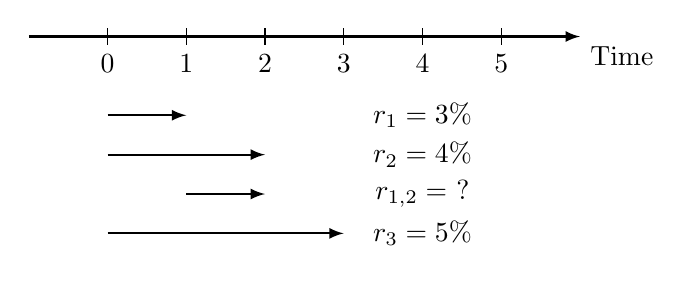
\begin{tikzpicture}
            % Draw the main number line
            \draw[thick, -latex] (-1,0) -- (6,0) node[anchor=north west] {Time};
            
            % Draw the spokes for 0-5
            \foreach \x in {0,...,5} {
              \draw (\x cm,3pt) -- (\x cm,-3pt) node[anchor=north] {$\x$};
            }
            
            % Draw the arrows 
            \draw[thick, -latex] (0,-1) -- (1,-1);
            \draw[thick, -latex] (0,-1.5) -- (2,-1.5);
            \draw[thick, -latex] (1,-2.0) -- (2,-2.0);
            \draw[thick, -latex] (0,-2.5) -- (3,-2.5);
            
            % Add labels
            \node at (4,-1) {$r_{1}=3\% $};
            \node at (4,-1.5) {$r_{2}=4\% $};
            \node at (4,-2.0) {$r_{1,2}= \ ?$};
            \node at (4,-2.5) {$r_{3}= 5 \% $};
        \end{tikzpicture}
        
    \end{figure}

    To get an intuitive idea for the forward rate calculation, we can say, if I am investing my money for a 2-year period (from years 0-2), this will be equivalent to investing for 1 year (from years 0-1), then reinvesting for another year (years 1-2) at the forward rate.


    \begin{align*}
        1.04^2 &= 1.03 \times (1 + r_{1,2}) \Rightarrow r_{1,2} = \frac{1.04^2}{1.03} - 1 = 5\%\\
        1.05^3 &= 1.04^2 \times (1 + r_{2,3}) \Rightarrow r_{2,3} = \frac{1.05^3}{1.04^2} - 1 = 7.03\% \\
               &= 1.03 \times 1.05 \times (1 + r_{2,3}) 
    \end{align*}


    Similarly:

    To find the forward rates, we can use the following relationships:

    \begin{align*}
        (1 + r_1)^1 &= (1 + r_1)(1 + r_{1,2}) \\
        (1 + r_2)^2 &= (1 + r_1)(1 + r_{1,2})(1 + r_{2,3}) \\
        (1 + r_3)^3 &= (1 + r_1)(1 + r_{1,2})(1 + r_{2,3})(1 + r_{3,4})
    \end{align*}

    Using these equations, we can solve for the forward rates:

    \begin{align*}
        (1 + 0.03)(1 + r_{1,2}) &= (1 + 0.04)^2 \\
        \Rightarrow\qquad r_{1,2} &= \frac{(1 + 0.04)^2}{(1 + 0.03)} - 1 = 5\%\\
        (1 + 0.04)^2(1 + r_{2,3}) &= (1 + 0.05)^3 \\
        \Rightarrow\qquad r_{2,3} &= \frac{(1 + 0.05)^3}{(1 + 0.04)^2} - 1 = 7.03\%
    \end{align*}


\end{examplebox}


\subsection*{Spot Rates in the Future - Theories}
There are three theories that try to explain and predict the yield curve:

\begin{itemize}
    \item Expectation Theory: The forward rate is the expected future spot rate. This is used in the calculation of forward rates.
    \begin{itemize}
                \item No risk premium: This theory assumes that investors do not demand a risk premium for holding long-term bonds, and that the forward rate is solely determined by the expected future spot rate.
                \begin{figure}[H]
                    \centering
                    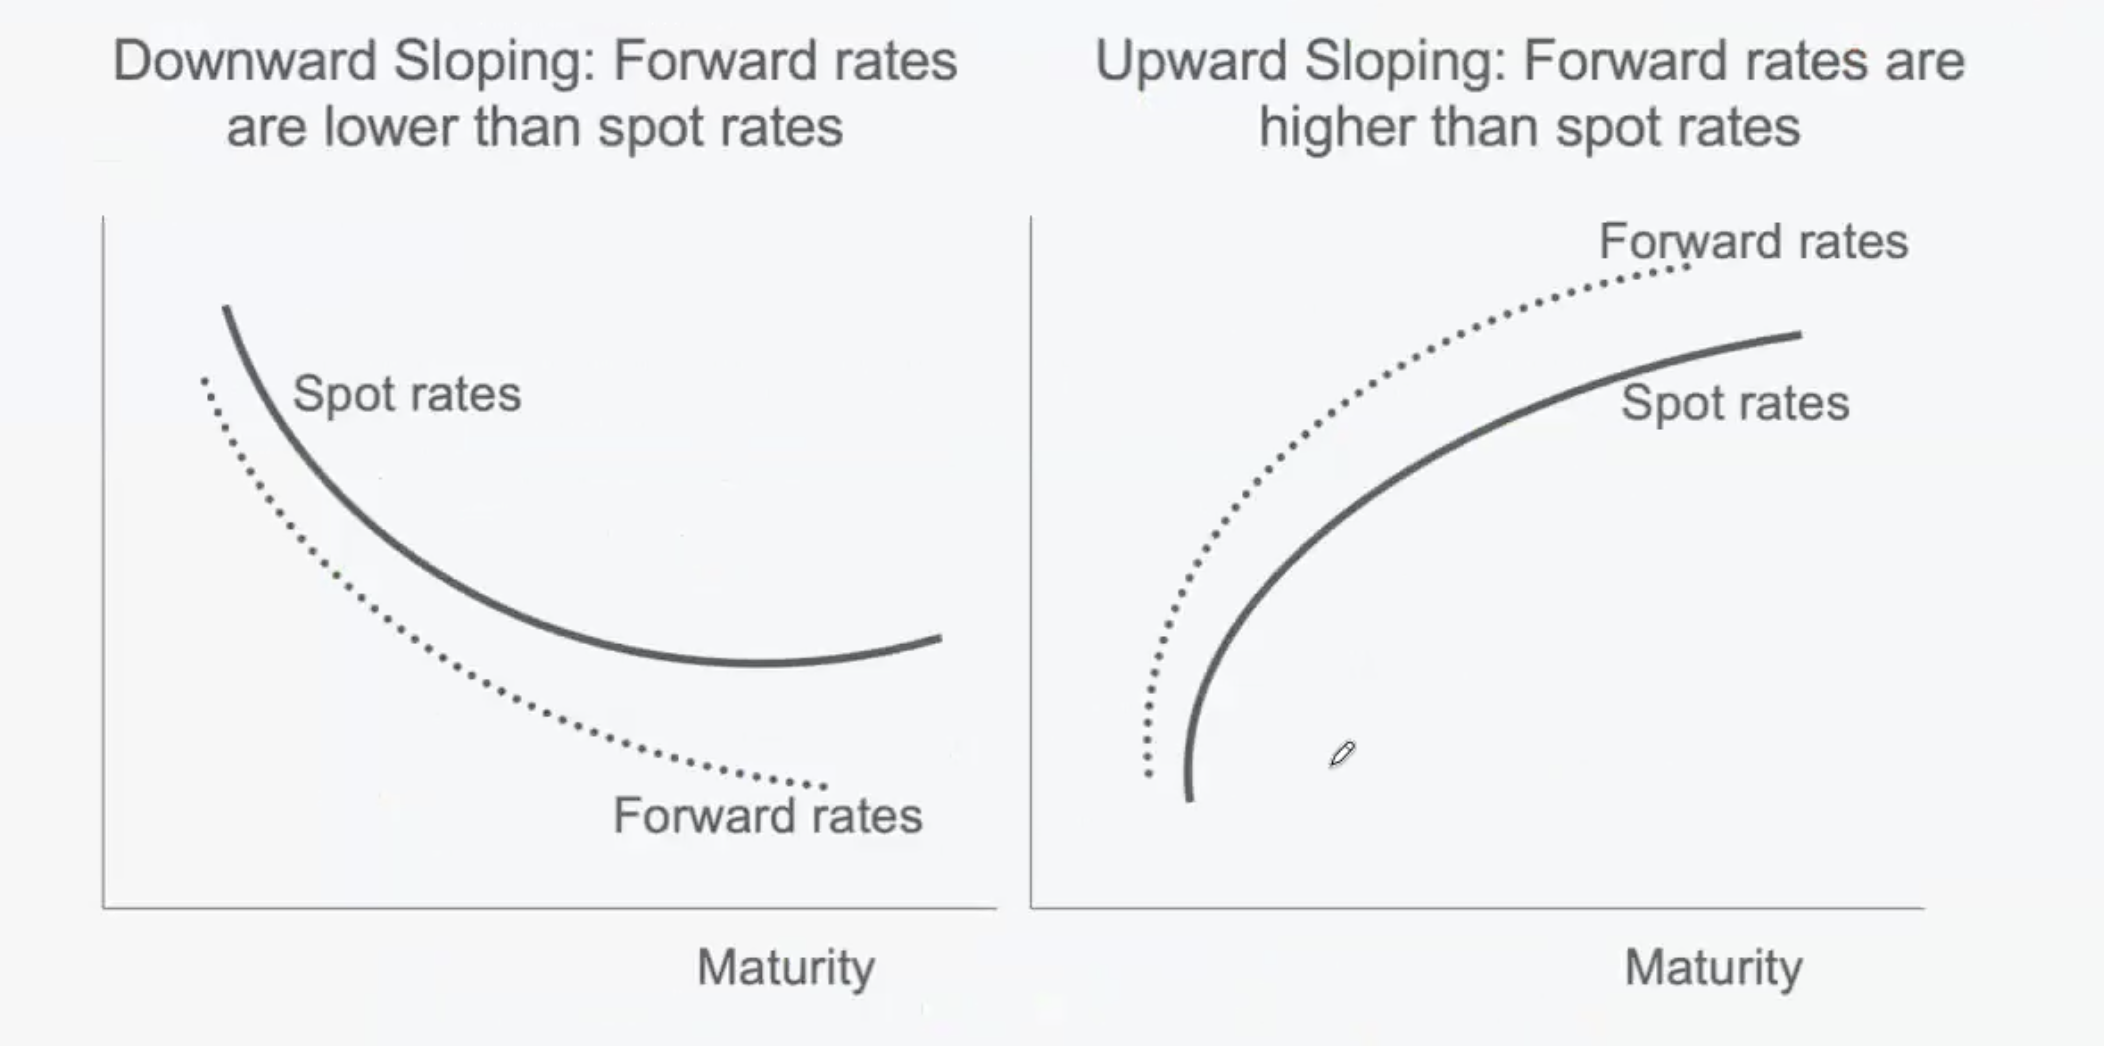
\includegraphics[width=0.8\textwidth]{img/2.5.png}
                \end{figure}
                \end{itemize}
    \item Liquidity Premium Theory:
    \begin{itemize}
                \item Long-term bonds are riskier than short-term bonds– This theory assumes that long-term bonds are riskier due to factors such as interest rate risk, credit risk, and liquidity risk.
                \item Investors demand a risk premium for holding long-term bonds: As a result, investors demand a higher return for holding long-term bonds, which leads to an upward-sloping yield curve.

    \end{itemize}
    \item Market Segmentation Theory:
    \begin{itemize}
                \item Bonds of different maturities are not substitutes: This theory assumes that bonds of different maturities are not perfect substitutes, and that investors have different preferences for bonds of different maturities.
                \item The supply and demand for bonds of each maturity determine the risk premium: The risk premium (and thus the yield curve) is determined by the supply and demand for bonds of each maturity, rather than by a single market-wide risk premium.
    \end{itemize}
\end{itemize}

\section{Corporate Bonds}
Prior to this section, government debt was discussed. Now this section focuses on corporate debt, which is more complex as corporations are potentially more likely to default than governments.

This is when a company fails to meet coupon payments, redemptions, or even financial distress such as liquidity shortages or going bankrupt. We rely on independent credit rating agencies like Moody's Fitch, and S\&P. They evaluate the quality of bonds based on credit quality assessing the likelihood of default over the bond's term. They provide qualitative ratings, for example, S\&P's:

\begin{itemize}
    \item AAA, AA, A, BBB: Investment Grade
    \item BB, B, CCC, CC, C: Speculative Grade
    \item D: Default
\end{itemize}

These ratings allow us to approximate the risk of default for a corporate bond. If a corporate bond has more credit risk (of default), investors will expect a higher yield to compensate for this risk. This is known as the credit spread, which is the difference between the yield on a corporate bond and the yield on a government bond of the same maturity.\\

The calculation of yield to maturity is similar as government debt, as the discount rate that equates the net present value of a bond's cash flow.

The credit ratings help use estimate average yield to maturity allowing us to plot yield curves for corporate bonds of varying risk levels and maturities.

\begin{figure}[H]
    \centering
    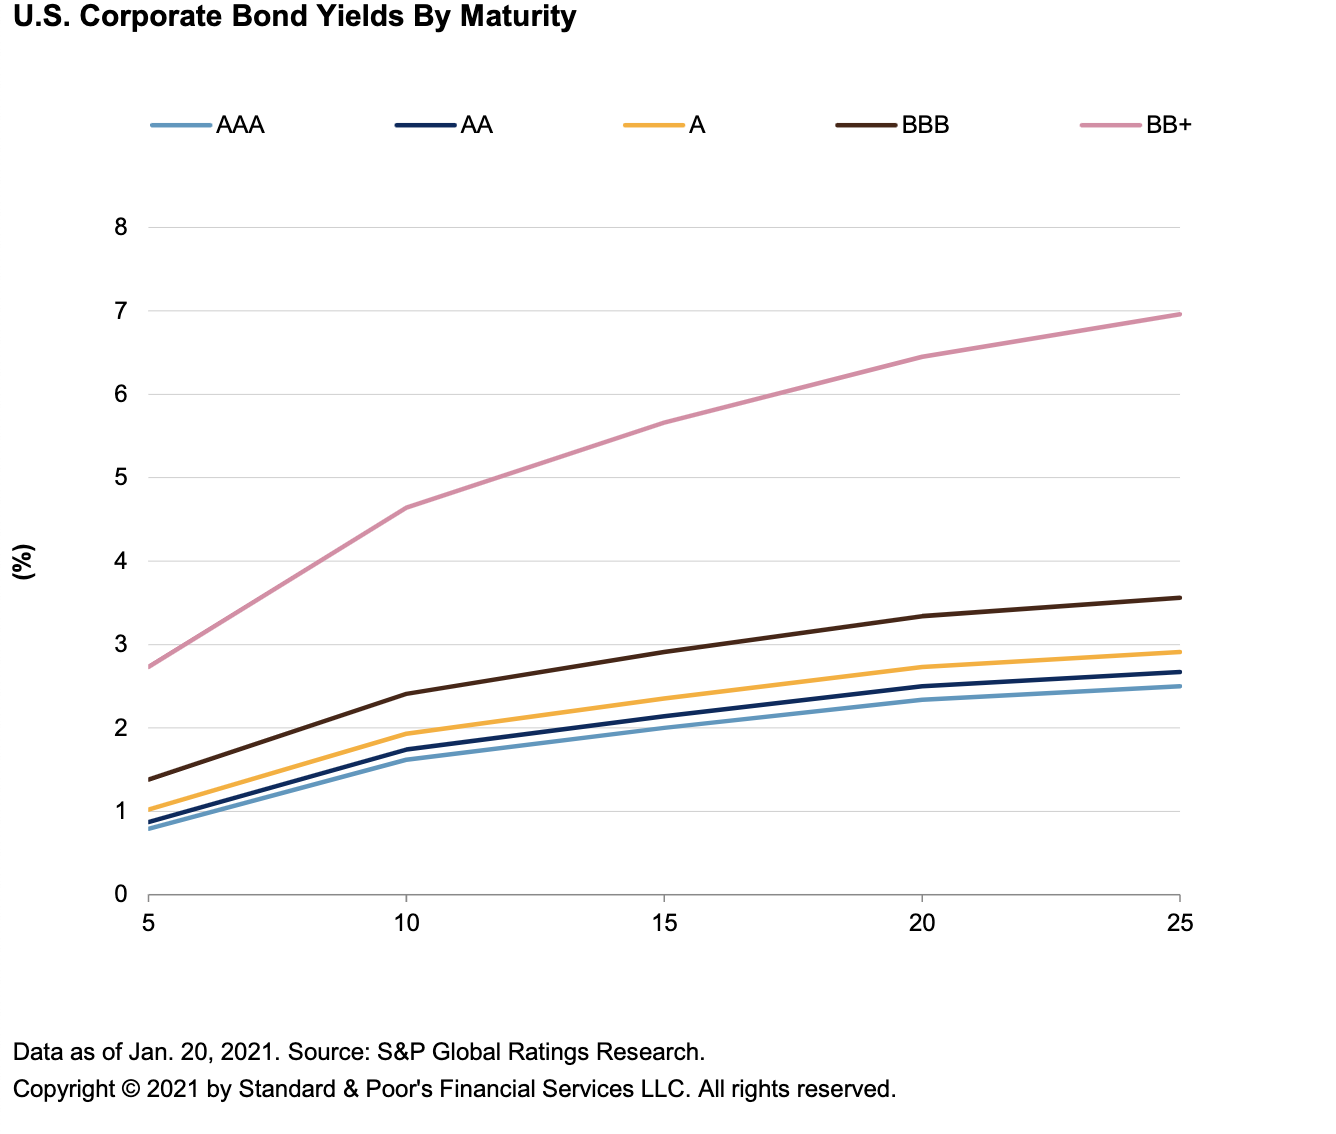
\includegraphics[width=0.5\textwidth]{img/2.6.png}
    \caption{Yield Curves for Corporate Bonds}
    \label{fig:corporate_yield_curve}
\end{figure}

In figure \ref{fig:corporate_yield_curve}, notice that moving down credit ratings, yields increase. The spread between the yields of corporate bonds serves as a gauge of credit risk. A wider spread indicates higher risk, with investors demanding higher yields to compensate for the increased risk of default.\\


\section{Green Bonds}
\begin{itemize}
    \item Green bonds are a financial instrument specifically to raise funds for environmentally-friendly projects, such as solar or wind farms, electric vehicle infrastructure or sustainable/efficient buildings.
    \item This allows investors to support projects that have a positive impact on the environment.
    \item Can be issue by governments, corporations, financial institutions, municipalities, banks, non-profits, and other entities.
    \item Can also be used to finance projects like reforestation, cleaning up or restoring habitats
\end{itemize}

\section{The Money Market}
\begin{sidenotebox}{The Money Market}

    \begin{itemize}
        \item Money markets offer \textbf{short-term, fixed-income instruments} with maturities of up to one year, facilitating the management of liquidity and short-term funding needs for firms, governments, and financial institutions.
        \item They function as a \textbf{large secondary market} for trading highly-liquid, short-term securities.
        \item Money markets provide a mechanism for entities to \textbf{manage surplus funds} efficiently and are a source of \textbf{low-cost short-term financing}.
        \item \textbf{Smaller investors} access these markets through \textbf{money market funds}, which are mutual funds that pool investors' funds to meet minimum capital requirements and achieve diversification.
        \item Unlike banks, which are \textbf{heavily regulated} and incur higher costs, money markets operate with \textbf{less regulatory oversight}, offering cost advantages especially in the trading of large sums.
    \end{itemize}
\end{sidenotebox}
    
\chapter{Equity Markets}
\renewcommand{\thesection}{3.1 - 3.2}
\section{Introduction and Key Concepts}
\setcounter{section}{2}
\renewcommand{\thesection}{\arabic{chapter}.\arabic{section}}

\begin{definitionbox}{Equity}
    The value of the ownership stake in a firm– the residual claim on the firm's assets after all other claims have been paid.
\end{definitionbox}

\begin{definitionbox}{Shares}
    Shares represent how the equity stake is divided. As a shareholder, you have right to claim portion of the company's profits, and control over the company's decisions.
\end{definitionbox}

These terms are sometimes used interchangeably, although they have slight differences.

\begin{itemize}
    \item Companies decide on the \textbf{allocation of profits} between reinvestment in the business and distribution as dividends, which are \textbf{distributed proportionately} to shareholders based on their shareholdings.
    \item The corporate structure and shareholder rights are established through \textbf{articles of association} (UK) or \textbf{articles of incorporation} (US), filed with Companies House in the UK or with the Secretary of State's office in the respective state in the US.
    \item Articles also delineate shareholder rights, including \textbf{voting and influence over management decisions}.
    \item As a company expands, it may \textbf{issue more shares to raise capital}, thus increasing the number of shareholders and shares in circulation.
    \item Some companies may decide to hold an \textbf{Initial Public Offering (IPO)}, which involves listing the company on a stock exchange, publicly.
    \item Shareholders exert control through a \textbf{voting process} in important company decisions such as issuing shares, debt management, and significant corporate actions like mergers and acquisitions.
    \item In the US, public companies are mandated to hold an \textbf{Annual General Meeting (AGM)}, where shareholders vote on crucial matters including the board of directors and executive compensation.
    \item There is a growing trend of shareholders influencing a company's \textbf{social and environmental practices}, asserting their rights and preferences in corporate governance.
    \item Active participation in voting and discussions at shareholder meetings helps \textbf{shape the company's direction and governance}.
\end{itemize}

\begin{enumerate}
    \item \textbf{Ownership vs. Creditship}
    \begin{itemize}
        \item Shares represent ownership in a company, providing rights to profits and decision-making.
        \item Bonds are debt obligations; bondholders are creditors, lending money without ownership rights.
        \item Shareholders have voting rights and participate in decisions like elections and mergers.
        \item Bondholders typically do not have voting rights, reflecting their role as lenders.
    \end{itemize}

    \item \textbf{Tax Treatment}
    \begin{itemize}
        \item Interest payments to bondholders are tax-deductible as business expenses, reducing taxable income.
        \item Dividends to shareholders are paid from after-tax profits and are not deductible.
    \end{itemize}

    \item \textbf{Priority of Payments or Seniority}
    \begin{itemize}
        \item In bankruptcy, bondholders have higher claim priority on assets than shareholders.
        \item Shareholders are residual claimants, receiving assets only after all creditors are paid.
    \end{itemize}

    \item \textbf{Risk and Return}
    \begin{itemize}
        \item Shares offer potential high returns but come with higher risks, including losses.
        \item Bonds provide stable returns through interest payments and principal repayment on maturity.
    \end{itemize}

    \item \textbf{Credit Risk}
    \begin{itemize}
        \item Bondholders have legal recourse (the right to take legal action) in defaults, able to reclaim their investment.
        \item Shareholders cannot demand dividends and must wait for company profitability to improve.
    \end{itemize}
\end{enumerate}


\begin{examplebox}{True or False?}

\begin{figure}[H] 
        \footnotesize
        \centering
        \begin{tabular}{|p{2.8cm}|p{2.8cm}|p{2.8cm}|p{2.8cm}|p{2.8cm}|}          
        \hline
        \textbf{Question} & \textbf{Option 1} & \textbf{Option 2} & \textbf{Option 3} & \textbf{Option 4} \\
        \hline
        Which of the following statements correctly relates to shares or shareholders? & 
        Ordinary shares represent the equity share capital of the firm. \textbf{True} & 
        Ordinary shareholders are the last in the queue to have their claims met. \textbf{True} & 
        Shareholders have the right to exercise control over the company. \textbf{True}& 
        The shareholder will always receive back the original capital invested. \textbf{False} \\
        \hline
        Which of the following statements best describe a company’s debt capital holders? & 
        They will always receive back their original capital. \textbf{False} & 
        They have no formal control. \textbf{True}& 
        They receive interest and may recover capital. \textbf{True} & 
        They have an equity interest in the company. \textbf{False}\\
        \hline
        Which of the following statements best describe the costs of equity when compared with debt capital? & 
        Equity finance is less expensive for companies. \textbf{False} & 
        Investing via debt finance is less risky for investors. \textbf{True}& 
        Investing via equity finance is less risky for investors. \textbf{False}& 
        Debt finance is less expensive for companies. \textbf{True}\\
        \hline
        Which of the following statements accurately describe the taxation of dividends and loans? & 
        Dividends are paid out of after-tax earnings. \textbf{True} & 
        The company will generally prefer equity finance since it is more tax-efficient. \textbf{False}& 
        Dividends can be used to reduce a firm’s taxable profits.\textbf{False} & 
        Interest payments on a loan are tax deductible. \textbf{True} \\
        \hline
        \end{tabular}
        \caption{Comparison of Shareholder and Debt Holder Attributes}
        \label{table:share_debt}

\end{figure}

\end{examplebox}



\section{Introduction to Equity Valuation}
There are three primary approaches to valuing shares:

\begin{itemize}
    \item \textbf{Dividend Discount Model (DDM):} 
    \begin{itemize}
        \item This model takes a directly estimates the present value of expected dividends. 
        \item The value of a share is derived from the present value of anticipated dividend payments. 
        \item Since dividends are uncertain and not predetermined, their expected values are considered.
    \end{itemize}
    
    \item \textbf{Discounted Cash Flow (DCF) Modelling:} 
    \begin{itemize}
        \item Widely employed by equity analysts, this indirect approach focuses on valuing the entire firm first. 
        \item This valuation is determined by discounting the expected future cash flows generated by the company. 
        \item After valuing the enterprise, all liabilities, such as debts and leases, are deducted from the enterprise value. 
        \item The residual amount, attributed to the shareholders, is then divided by the number of shares to provide the value per share. 
    \end{itemize}
    
    \item \textbf{Multiples Approach:} 
    \begin{itemize}
        \item This method estimates the value of a company by comparing it to similar companies in the market using financial ratios or multiples, such as the price-to-earnings ratio (P/E) or the enterprise value-to-EBITDA (EV/EBITDA). 
        \item Multiples valuation is a quick and straightforward approach, relying on market-based data and the performance of similar companies.
    \end{itemize}
\end{itemize}


\subsection*{Dividend Discount Model}
\begin{definitionbox}{Dividend Discount Model}
\textbf{Assumptions:}
\begin{enumerate}
    \item \textbf{Zero-Growth Dividend Model: }\\Assume dividend stream is constant over time, like a zero-growth perpetuity. Assume first dividend payment is received one year from now.
    \begin{equation}
        P_0 \text{ (current price of the stock)}= \frac{D_1 \text{ (expected dividend payment)}}{r \text{ (required rate of return on equity or cost of equity)}}
    \end{equation}
    \item \textbf{Constant-Growth Dividend Model (Gordon Growth Model): }\\Assume dividend stream will grow at a constant rate indefinitely into the future, like a growing perpetuity.
    \begin{equation}
        P_0 \text{ (current price of the stock)}= \frac{D_1 \text{ (the expected payment at the end of the upcoming period)}}{r \text{ (cost of equity)} - g \text{( the growth rate of dividends)}}
    \end{equation}
    \item \textbf{Multi-Period Dividend Model (Dividend Discount Model for Multiple Periods): }\\Assumption (involving having information about dividends for the next $n$ years) that either the dividend stream remains constant or grows at a constant rate. Thus, the value of the stock is calculated as such
    \begin{equation}
        P_0 = \frac{D_1}{(1+r)} + \frac{D_2}{(1+r)^2} + \ldots + \frac{D_n}{(1+r^n)} + \frac{\frac{D_n \times (1+g)}{(r-g)}}{(1+r)^n}
    \end{equation}
\end{enumerate}

\textbf{Do note that these models only price a stock based on dividend cash flows and do not consider other factors like capital gains, etc.}

\end{definitionbox}

\begin{examplebox}{Bits 'n' Pieces Stock Return}
    Bits ‘n’ Pieces pays a constant annual dividend of £0.50 a share. The market price of the stock is £5.41 today. What is the rate of return on this stock?
    
    The rate of return can be calculated using the formula:
    \begin{align*}
        r_E &= \frac{\text{Div}}{P_0} \\
        &= \frac{0.50}{5.41} \\
        &= 0.09242 \\
        &= 9.24\%
    \end{align*}
    Therefore, the rate of return on this stock is 9.24\%.
\end{examplebox}

\begin{examplebox}{JLE Inc Stock Valuation}
    JLE, Inc. just paid its annual dividend of £1.10 a share. JLE’s policy is to increase the dividend by 2\% annually. How much are you willing to pay today for a share of this stock if you require an 11\% rate of return?
    
    The present value of the stock can be calculated as:
    \begin{align*}
        P_0 &= \frac{Div_1}{r_E - g} = \frac{Div_0 \times (1 + g)}{r_E - g} \\
        &= \frac{1.10 \times (1 + 0.02)}{0.11 - 0.02} \\
        &= \frac{1.122}{0.09} \\
        &= 12.46667 \\
        &\approx £12.47
    \end{align*}
    Hence, you would be willing to pay approximately £12.47 for a share of this stock.
\end{examplebox}

\begin{examplebox}{Isaac's Shoes Stock Valuation}
    Isaac’s Shoes just announced that it will commence paying annual dividends next year. The plan is to pay £0.50, £0.75 and £1.00 per share over the next three years, respectively. After that, the company plans on increasing the dividend by 2.5\% annually. The market rate of return on this stock is 12.5\%. What should the market price of this stock be?
    
    To calculate the market price of the stock, we use:
    \begin{align*}
        P_3 &= \frac{Div_4}{r_E - g} = \frac{Div_3 \times (1 + g)}{r_E - g} \\
        &= \frac{1.00 \times (1 + 0.025)}{0.125 - 0.025} \\
        &= \frac{1.025}{0.10} \\
        &= 10.25
    \end{align*}
    And then we discount the dividends and the price $P_3$ to the present value:
    \begin{align*}
        P_0 &= \frac{Div_1}{(1 + r_E)} + \frac{Div_2}{(1 + r_E)^2} + \frac{Div_3}{(1 + r_E)^3}+\frac{\frac{Div_3 \times (1 + g)}{r_E - g}}{(1 + r_E)^3}  \\
         &= \frac{Div_1}{(1 + r_E)} + \frac{Div_2}{(1 + r_E)^2} + \frac{Div_3 + P_3}{(1 + r_E)^3} \\
        &= \frac{0.50}{(1 + 0.125)} + \frac{0.75}{(1 + 0.125)^2} + \frac{1.00 + 10.25}{(1 + 0.125)^3} \\
        &= 0.44444 + 0.59259 + 7.90123 \\
        &= 8.93826 \\
        &= £8.94
    \end{align*}
    Therefore, the market price of Isaac’s Shoes stock should be £8.94.
    \end{examplebox}
    
    \begin{examplebox}{Flo's Home Furnishings Required Return}
        The common stock of Flo’s Home Furnishings has a 3.5\% dividend yield. You expect the company to grow by 6\% annually. What is the required return on this stock?
        
        The required return can be computed using the formula:
        \begin{align*}
            r_E &= \frac{Div_1}{P_0} + g \\
            &= 3.5\% + 6\% \\
            &= 9.5\%
        \end{align*}
        Thus, the required return on this stock is 9.5\%.
        \end{examplebox}
             
        \begin{examplebox}{Supernormal Growth Stock Valuation}
            Suppose a firm is expected to increase dividends by 20\% in one year and by 15\% in two years. After that, dividends will increase at a rate of 5\% per year indefinitely. If the last dividend was £1 and the required return is 20\%, what is the price of the stock? Remember we have to find the present value of all expected future dividends.
            
            We calculate the supernormal growth dividends and then the price:
            \begin{align*}
                Div_1 &= 1 \times (1.2) = £1.20 \\
                Div_2 &= 1.20 \times (1.15) = £1.38 \\
                Div_3 &= 1.38 \times (1.05) = £1.449 \\
            \end{align*}
            The expected future price (at the end of year 2) is:
            \begin{align*}
                P_2 &= \frac{Div_3}{r_E - g} = \frac{1.449}{0.20 - 0.05} = 9.66
            \end{align*}
            Finally, we find the present value of the expected future cash flows:
            \begin{align*}
                P_0 &= \frac{Div_1}{(1 + r_E)} + \frac{Div_2}{(1 + r_E)^2} + \frac{Div_3 + \frac{Div_3 \times (1+g)}{r_E - g}}{(1 + r_E)^3}\\
                P_0 &= \frac{Div_1}{(1 + r_E)} + \frac{Div_2}{(1 + r_E)^2} + \frac{Div_3 + P_2}{(1 + r_E)^3}\\
                    &= \frac{1.20}{1.2} + \frac{1.38}{1.2^2} + \frac{1.449 + 9.66}{1.2^3} \\
                &= 8.67
            \end{align*}
            The price of the stock, considering the supernormal growth, is £8.67.
        \end{examplebox}
            
\section{Equity Valuation}

\begin{itemize}
    \item Examine the diagram that illustrates the relationship between market prices and the required rate of return (cost of equity)
    \item Assume that annual aggregate dividend payout is £2M or $d=2$ and assume growth rate $g = 5\%$ which combines real economic growth and inflation and initial required rate of return $r = 10\%$.
    \begin{figure}[H]
        \centering
        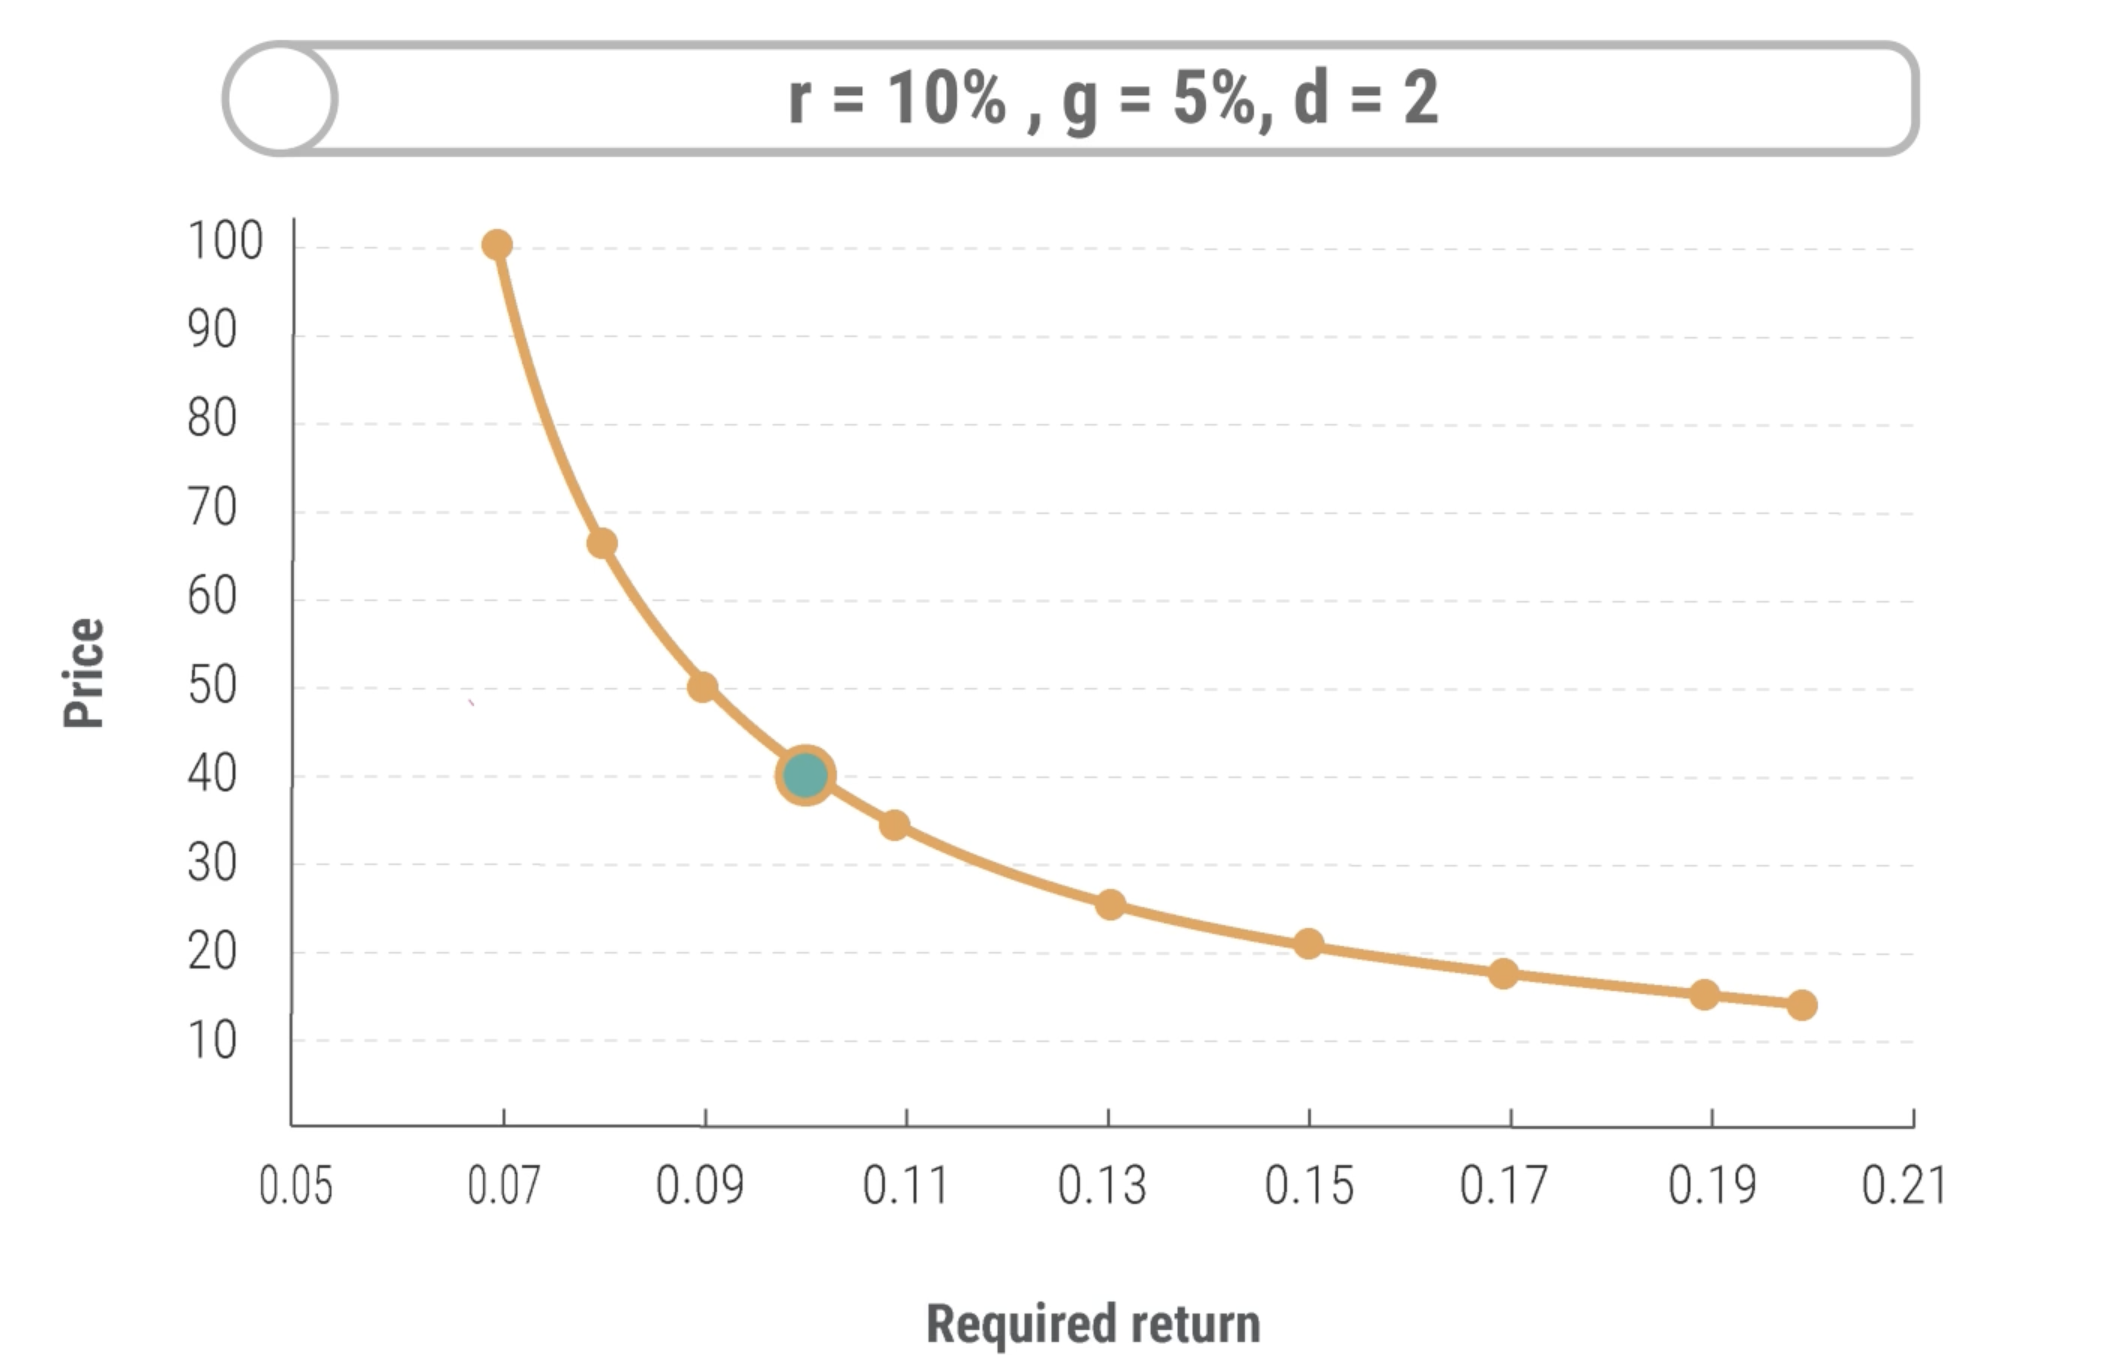
\includegraphics[width=0.5\textwidth]{img/3.4.1.png}
    \end{figure}
    \item Market value is calculated as the dividend $d=2$ divided by the difference between the required rate of return $r$ and the growth rate $g$. So the market value is $2/(0.10-0.05) = 40$.
    \item When there are positive or negative changes in market sentiment, the required rate of return may change, affecting the market value of the stock.
    \begin{figure}[H]
        \centering
        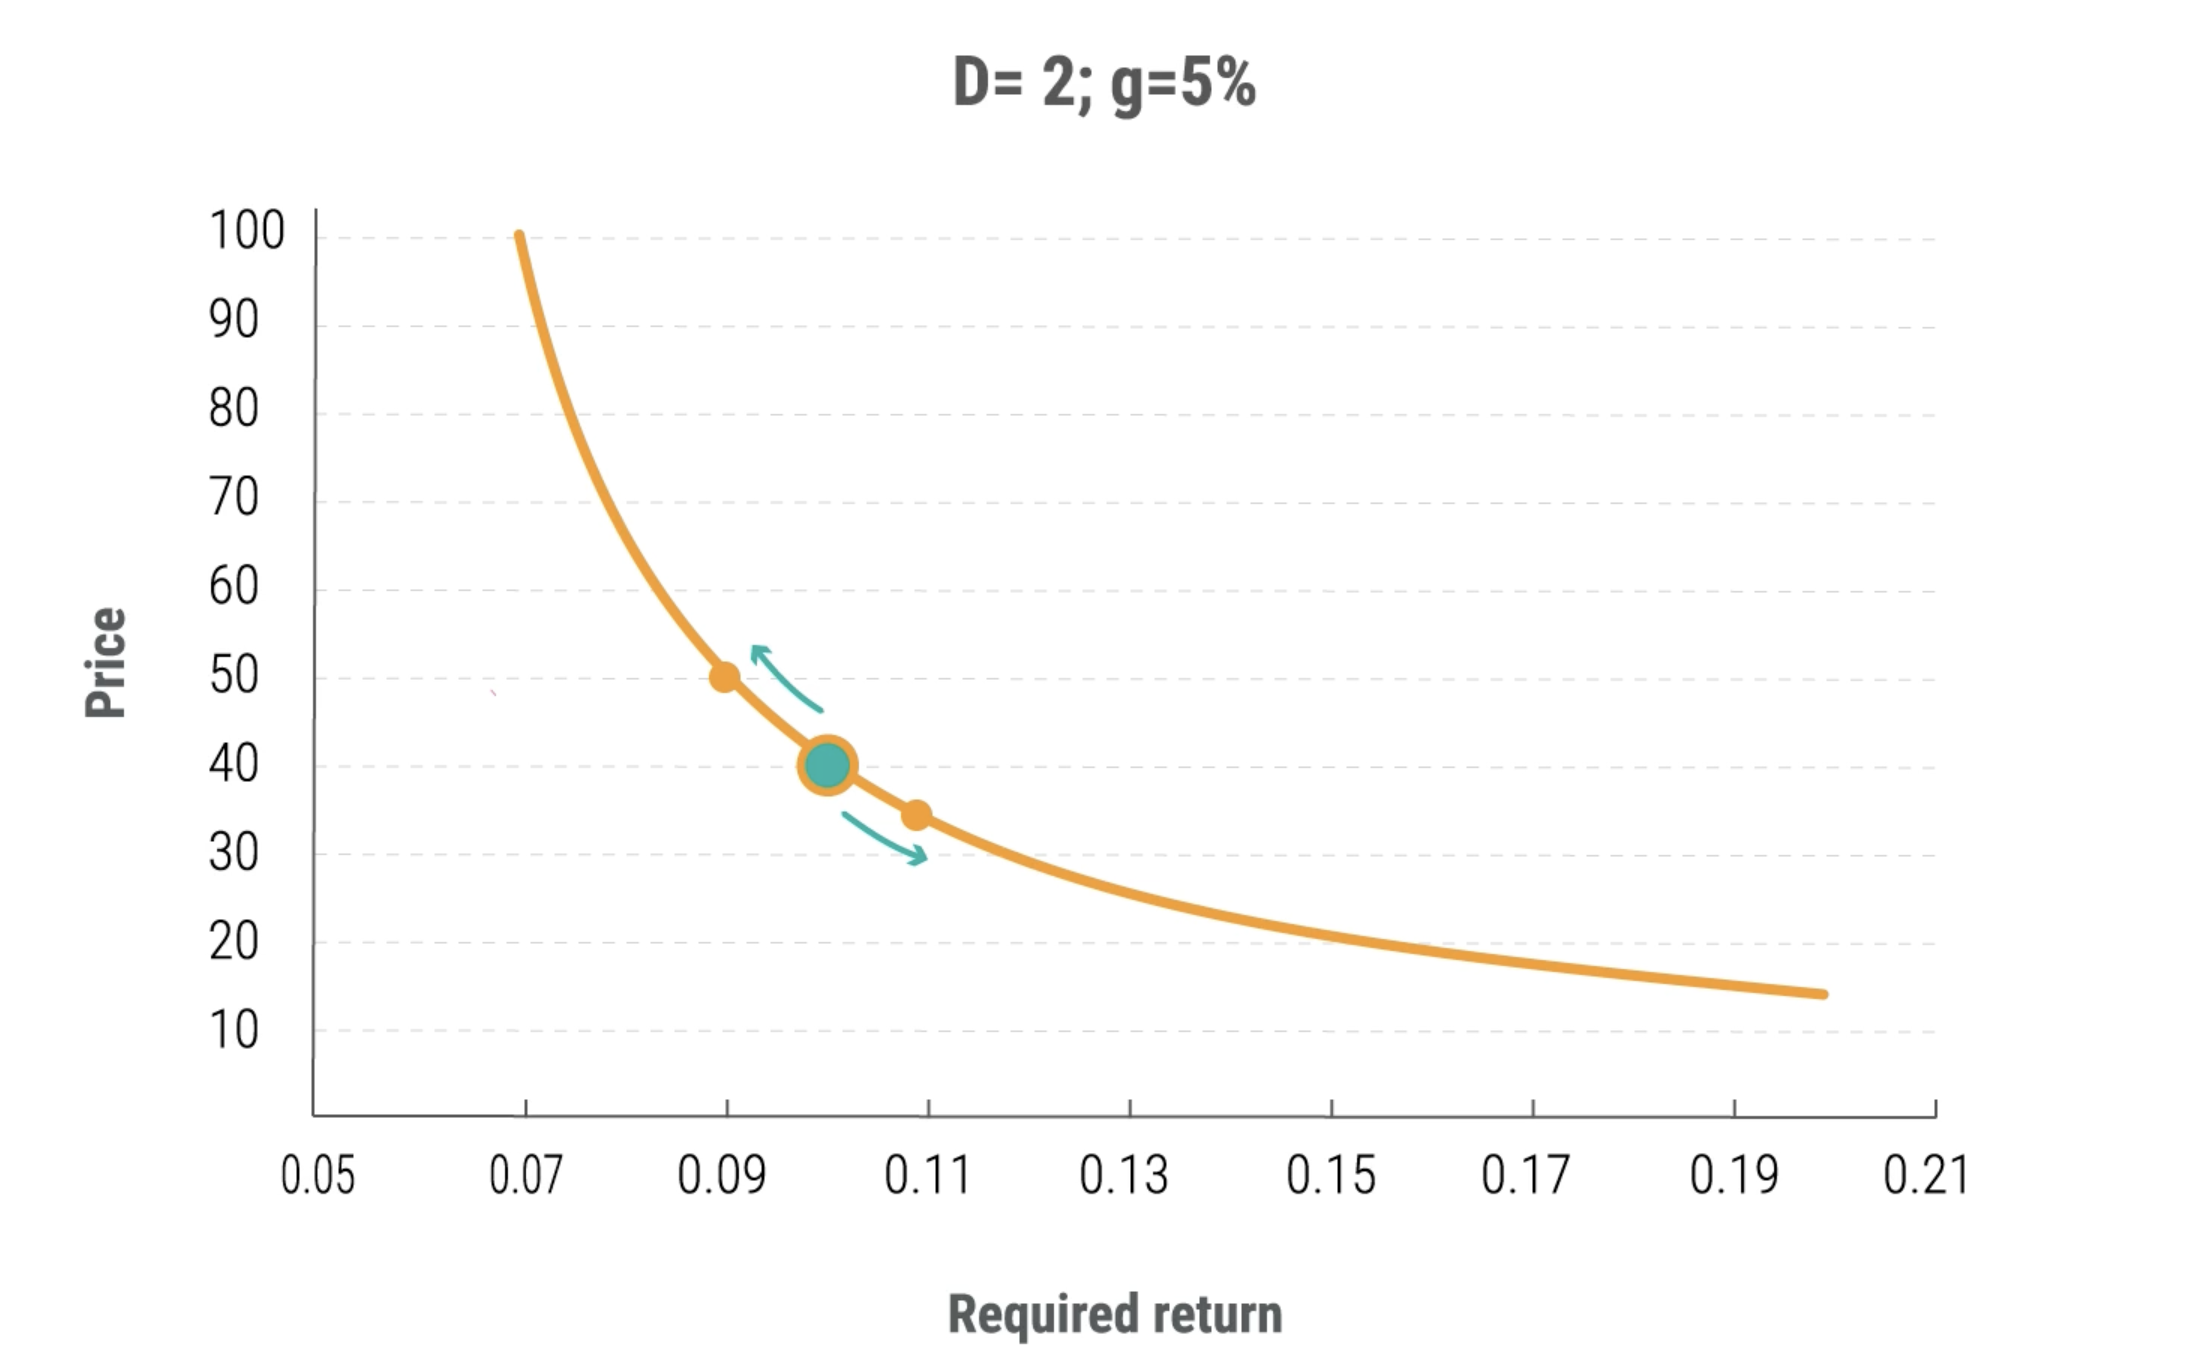
\includegraphics[width=0.5\textwidth]{img/3.4.2.png}
    \end{figure}
    \item A debt crisis may make investors more risk-averse and demand a higher rate of return which then reduces the market value/price of the stock.
    \item On the other hand, a positive economic outlook may reduce the required rate of return, increasing the market value/price of the stock.
    \item This simple model shows why markets can be so sensitive to changes in sentiment and expectations about the future.
    \item Shares are considered to have almost unlimited lifespans, which implies high sensitivity to small changes in the required rate of return, similar to (long-term) bonds that are sensitive to changes in interest rates.
\end{itemize}

We can manipulate the formula to find the required rate of return for a stock given its dividend $Div$, price $P$, and growth rate $g$. The formula is as follows:
\begin{equation}
    r_E = \underbrace{\frac{Div}{P}}_{\text{Dividend Yield} } + \underbrace{g}_{\text{Growth Rate}} 
\end{equation}

\begin{itemize}
    \item Assume that in a given year, the UK market had a dividend yield of 4.5\% and a growth rate of 5\%. Then, the required rate of return for the UK market would be 9.5\%.
\end{itemize}

\section{Case study: Shiller and Siegel}
\textbf{Reading Links:}
\begin{itemize}
    \item \href{https://www.ft.com/content/23c9f650-10c7-11e3-b5e4-00144feabdc0}{Clash of the Cape Crusaders: The world’s leading market historians are locked in an intense debate over the true value of stocks
    }
    \item \href{https://www.advisorperspectives.com/articles/2014/02/18/cape-crusaders-the-shiller-siegel-shootout-at-the-q-group-corral}{A breakdown of their debate}
    
    
\end{itemize}
\textbf{Summary}
\begin{itemize}
    \item \textbf{Robert Shiller} and \textbf{Jeremy Siegel} are two prominent economists with differing views on the stock market performance.
    \item \textcolor{blue}{Shiller, a Nobel laureate, is known for his work on the \textbf{Cyclically Adjusted Price Earnings (CAPE) ratio}, which compares stock prices to average earnings over the past 10 years.}
    \item \textcolor{red}{Siegel, a Wharton professor, is a proponent of the \textbf{efficient market hypothesis}, which posits that stock prices reflect all available information.}
    \item \textcolor{blue}{Shiller argues that the CAPE ratio is a reliable indicator of stock market valuation, suggesting that high ratios predict lower future returns.}
    \item \textcolor{red}{Siegel contends that the CAPE ratio is flawed, as it does not account for changes in accounting standards and the impact of low interest rates on stock prices.}
\end{itemize}

\textbf{Robert Shiller's Perspective (Market Overvalued)}
\begin{itemize}
    \item \textbf{Cyclically Adjusted Price/Earnings (CAPE) Ratio:} Shiller utilises the CAPE ratio, which averages earnings over 10 years to smooth out fluctuations and adjusts for inflation. This method is designed to provide a more stable and historically grounded measure of stock market valuation, indicating when stocks are cyclically high or low.
    \item \textbf{Behavioural Finance Insights:} Shiller, being a proponent of behavioural finance, argues that psychological factors often drive market errors. He believes that the current high readings of the CAPE ratio reflect an overvalued market driven by investor psychology rather than underlying economic fundamentals.
    \item \textbf{Historical Context and Mean Reversion:} Shiller points to historical trends where the CAPE ratio has reverted to the mean after extreme highs, suggesting that periods of high CAPE values are often followed by market corrections or crashes.
\end{itemize}

\textbf{Jeremy Siegel's Perspective (Market Undervalued)}
\begin{itemize}
    \item \textbf{Revised CAPE Ratio:} Siegel has proposed modifications to the CAPE ratio, arguing that changes in accounting practices and economic conditions over time have rendered the traditional CAPE ratio based on Shiller’s model as outdated and pessimistic. Siegel’s adjustments suggest that the market is currently undervalued rather than overvalued.
    \item \textbf{Long-term Stock Market Trends:} Siegel emphasises the historical performance of stocks, noting that over long periods, equities have tended to outperform other asset classes even when adjusted for inflation. This underpins his belief in the "buy-and-hold" strategy, suggesting that fears of overvaluation may be overstated.
    \item \textbf{Optimism about Earnings Growth:} Siegel also points to a trend of increasing earnings growth since World War II, driven by companies retaining more earnings rather than paying them out as dividends. This, he argues, should lead to a higher equilibrium CAPE ratio, implying that the stock market can sustain higher valuation levels without being overvalued.
\end{itemize}

\section{Features of common stock and preferred shares}

Companies may issue multiple classes of stock, which can have different voting rights and privileges.
Common stockholders typically have the right to vote on company matters, while preferred stockholders may not possess voting rights but receive preferential treatment in terms of dividend payments or liquidation proceeds.

Different classes of stock enable companies to offer various rights and benefits to different shareholders. 

\begin{itemize}
    \item \textbf{Voting Rights: }Shares give ownership rights in relation to how the company is run. These rights are invariably exercised through voting at shareholder meetings, e.g. the Annual General Meeting (AGM).
    \item \textbf{Proxy Voting: }Proxy voting is a mechanism where shareholders delegate their voting rights to another party. Historically, fund managers nominated the board of directors as their proxy, but this is now changing, as fund managers want to be more active in matters relating to company decision-making.
    \item \textbf{Classes of Stock: }Some firms have different classes of common stock. These classes often differ in their voting rights — for example, Moller - Maersk has A and B shares, but only class A shareholders have voting rights.
    \item \textbf{Other Rights: }
    \begin{itemize}
        \item The proportion received in declared dividends and/or remaining assets during liquidation. (Some shares get more or less of dividends and liquidated assets)
        \item Pre-emptive rights — the first ‘option to buy’ a new stock issue is offered to existing shareholders
        \item Since 2006, this option-to-buy right has been required by UK law, unless shareholders have actively voted to drop the provision. This is not the case in the USA.
    \end{itemize}
    \item \textbf{Dividend Characteristics: }
    \begin{itemize}
        \item Dividends are not a liability of the firm until they have been declared by the board.
        \item Consequently, a firm cannot go bankrupt for not paying any dividends.
        \item Dividends are paid out of post-tax earnings; they are not tax-deductible.
    \end{itemize}
\end{itemize}


\section{Market Efficiency}

\begin{itemize}
    \item Efficient capital markets are a theoretical model of how financial markets operate under certain conditions, assuming all information is freely available and there are no trading costs.
    \item Market efficiency means that all available information is fully reflected in security prices, making it impossible for investors to consistently earn above-average returns for a given level of risk.
    \item In an efficiently functioning market, securities with equal risk should deliver the same return after adjusting for their respective levels of risk.
    \item Market efficiency is divided into three categories based on the information sets we consider:
    
    \begin{enumerate}
        \item \textbf{Weak Form Efficiency: } 
        \begin{itemize}
            \item Based on historical prices only, implying that past prices are already incorporated into current prices. 
            \item An investor relying solely on this information cannot consistently outperform the market. 
            \item Strategies based on technical analysis or momentum trading, where investors chase past price trends, tend to underperform in this context.
        \end{itemize}

        \item \textbf{Semi-Strong Form Efficiency: } 
        \begin{itemize}
            \item Incorporates all publicly available information, including financial statements, news, accounting data, and other data.
            \item It means that even strategies that incorporate any or a combination of fundamental analysis (accounting information) or price data, find it challenging  to outperform the market.
        \end{itemize}
        \item \textbf{Strong Form Efficiency: }
        \begin{itemize}
            \item In the most idealised scenario, all information (including those mentioned above), both private and public, is factored into market prices. In wallstreetbets lingo, everything is \textit{priced in}.
            \item This is rarely believed in practice, as individuals with inside information can sometimes outperform the market (therefore we cannot assume everyone has access to all information).
            \item What really matters is, thus, whether the market is
            semi-strong efficient or weak form efficient.
        \end{itemize} 
    \end{enumerate}

\end{itemize}



\chapter{Valuation of a Firm}

\section{Introduction}
\begin{itemize}
    \item Recap of the previous session on the dividend discount model (DDM):
      \begin{itemize}
        \item We valued shares based on present value of expected dividends.
        \item We discussed its applicability for mature companies with consistent dividend payouts.
        \item Noted limitations due to the variable nature of dividends.
      \end{itemize}
    \item Introduction to the Discounted Cash Flow (DCF) method:
      \begin{itemize}
        \item Popular among equity research analysts for its flexibility.
        \item Allows for detailed company analysis including scenario testing.
      \end{itemize}
  \end{itemize}

\section{Estimating enterprise value}
A DCF calculates projected future cash flows from company. Projection can be done based on historical data, industry trends, and management forecasts. Next, we must determine the discount rate which is the required rate of return.\\

Discount rate is calculated using weighted average cost of capital (WACC), which takes into account the cost of equity and cost of financing/debt.

Once cash flows and discount rate are determined, the next step is calculating the present value of each projected cash flow (using the discounted rate). The sum of these present values is the enterprise value of the company. Let $r$ be the discount rate, $CF$ be the cash flow, and $n$ be the number of time periods. The present value of cash flow is given by:

\begin{equation}
    PD  = \frac{CF}{(1+r)^n}
\end{equation}

In many cases the projected cash flows extend for a finite period. To account for the value beyond the projected period, a terminal value is used at the end of that period, which assumes a constant growth rate. The terminal value (TV) is calculated as \textbf{Gordon Growth Model}:

\begin{equation}
    TV = \frac{CF_{n+1}}{r-g}
\end{equation}

(There is also an exit multiple method, which uses a multiple of EBITDA or EBIT to calculate terminal value.)

This terminal value is discounted back to its present value using the discount rate. 

Add the present projected value and the present terminal value to get the enterprise value (V).

\begin{equation}
    V = \sum_{i=1}^{n} \frac{CF_i}{(1+r)^i} + \frac{CF_{n+1}}{r-g}
\end{equation}

Calculate the share price or equity value: deduct the net debt from the enterprise value and divide by the number of shares outstanding. Equity value is the firm's value V, minus any liabilities (in our simplified model all liabilities are just debt).

\begin{equation}
    \text{Equity Value } E = \frac{V - \text{Net Debt } D}{\text{Shares Outstanding}}
\end{equation}

Two valuation approaches (DDM) and (DCF) are both used. DDM is problematic when companies have a discretionary dividend policy, or when they have a high growth rate. DCF is more flexible and practical as it can be used for companies with no dividends, or when dividends are not a good indicator of company performance. This is because it incorporates all cash flows to estimate the company's enterprise value.\\

For DCF to work, cash flow estimations must be accurate. \textbf{Assume the company is 100\% equity financed for now.} \\

Focusing on the income statement, note the free cash flow, generated for all capital lenders to the firm (debt and equity). 

\subsection*{EBIT (Earnings Before Interest and Tax)}
\begin{equation}
    EBIT = \text{Revenue} - \text{Operating Expenses}
\end{equation}

Not all cash flows are available to investors, as the company must pay taxes and cover other costs to reinvest into the business. So the free cash flow is calculated as:

\begin{align}
    \text{Total Cash Flow } &= EBIT (1-t) + \text{Depreciation}\\
    \text{Free Cash Flow } &= EBIT (1-t) + \text{Depreciation} - \text{Capital Expenditure} - \text{Change in Net Working Capital (NWC)}\\
    &= \text{Total Cash Flow} - \text{Capital Expenditure} - \text{Change in Net Working Capital (NWC)}
\end{align}

If the company is partially debt-financed, the cost of debt must be accounted for as the company's tax bill is less due to tax exemption on debt. This adjustment is made in the discount rate which is lowered to account for the tax shield. This discount rate is the WACC, or the weighted average cost of capital.\\

A terminal value is calculated at the end of the projection period, similar to the DDM. A constant growth rate is assumed for the terminal value. 

\begin{equation}
    TV = \frac{FCF_{N+1}}{r_{WACC}-g}
\end{equation}

\begin{equation}
    FCF_{N+1} = FCF_N^*(1+g)
\end{equation}

\renewcommand{\thesection}{4.3 - 4.5}
\section{Calculating Enterprise Value}
\setcounter{section}{5}
\renewcommand{\thesection}{\arabic{chapter}.\arabic{section}}

\subsection*{Case Study: Apple}
\begin{itemize}
    \item 2012: Apple's stock was at \$700.
    \item 2014: 7-1 stock split, reducing the price to \$100.
    \item Apple felt the share price was too high, so it was split to improve liquidity
    \item Apple was one of the largest companies by market capitalisation in 2023, with a valuation of nearly \$2.8 trillion.
     \begin{figure}[H]
        \centering
        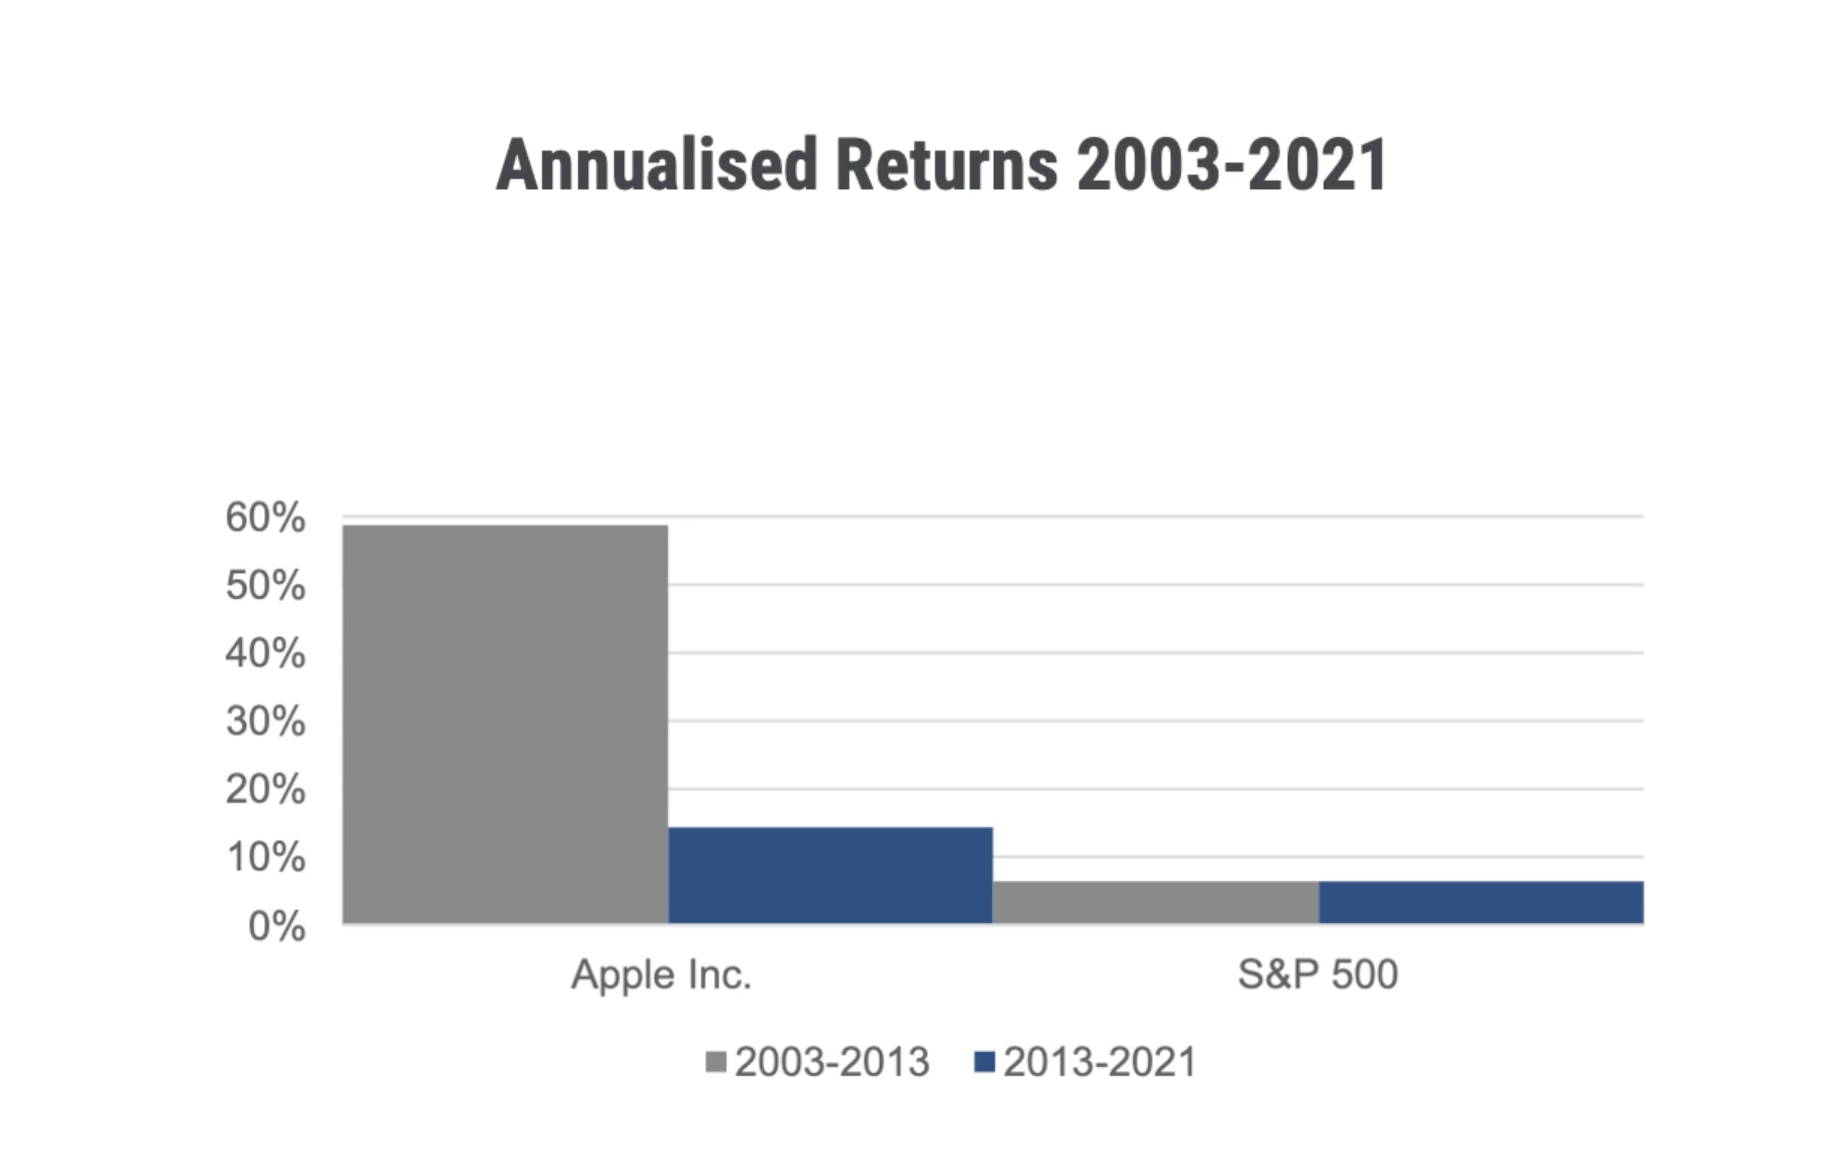
\includegraphics[width=0.5\textwidth]{img/4.3.png}
        \caption{Annualised returns 2003-2021}
    \end{figure}
    \item Apple is a tech giant and its success lies in the synergies of its products.
    \item To best value Apple, we must look at the aggregate level.
     \begin{figure}[H]
        \centering
        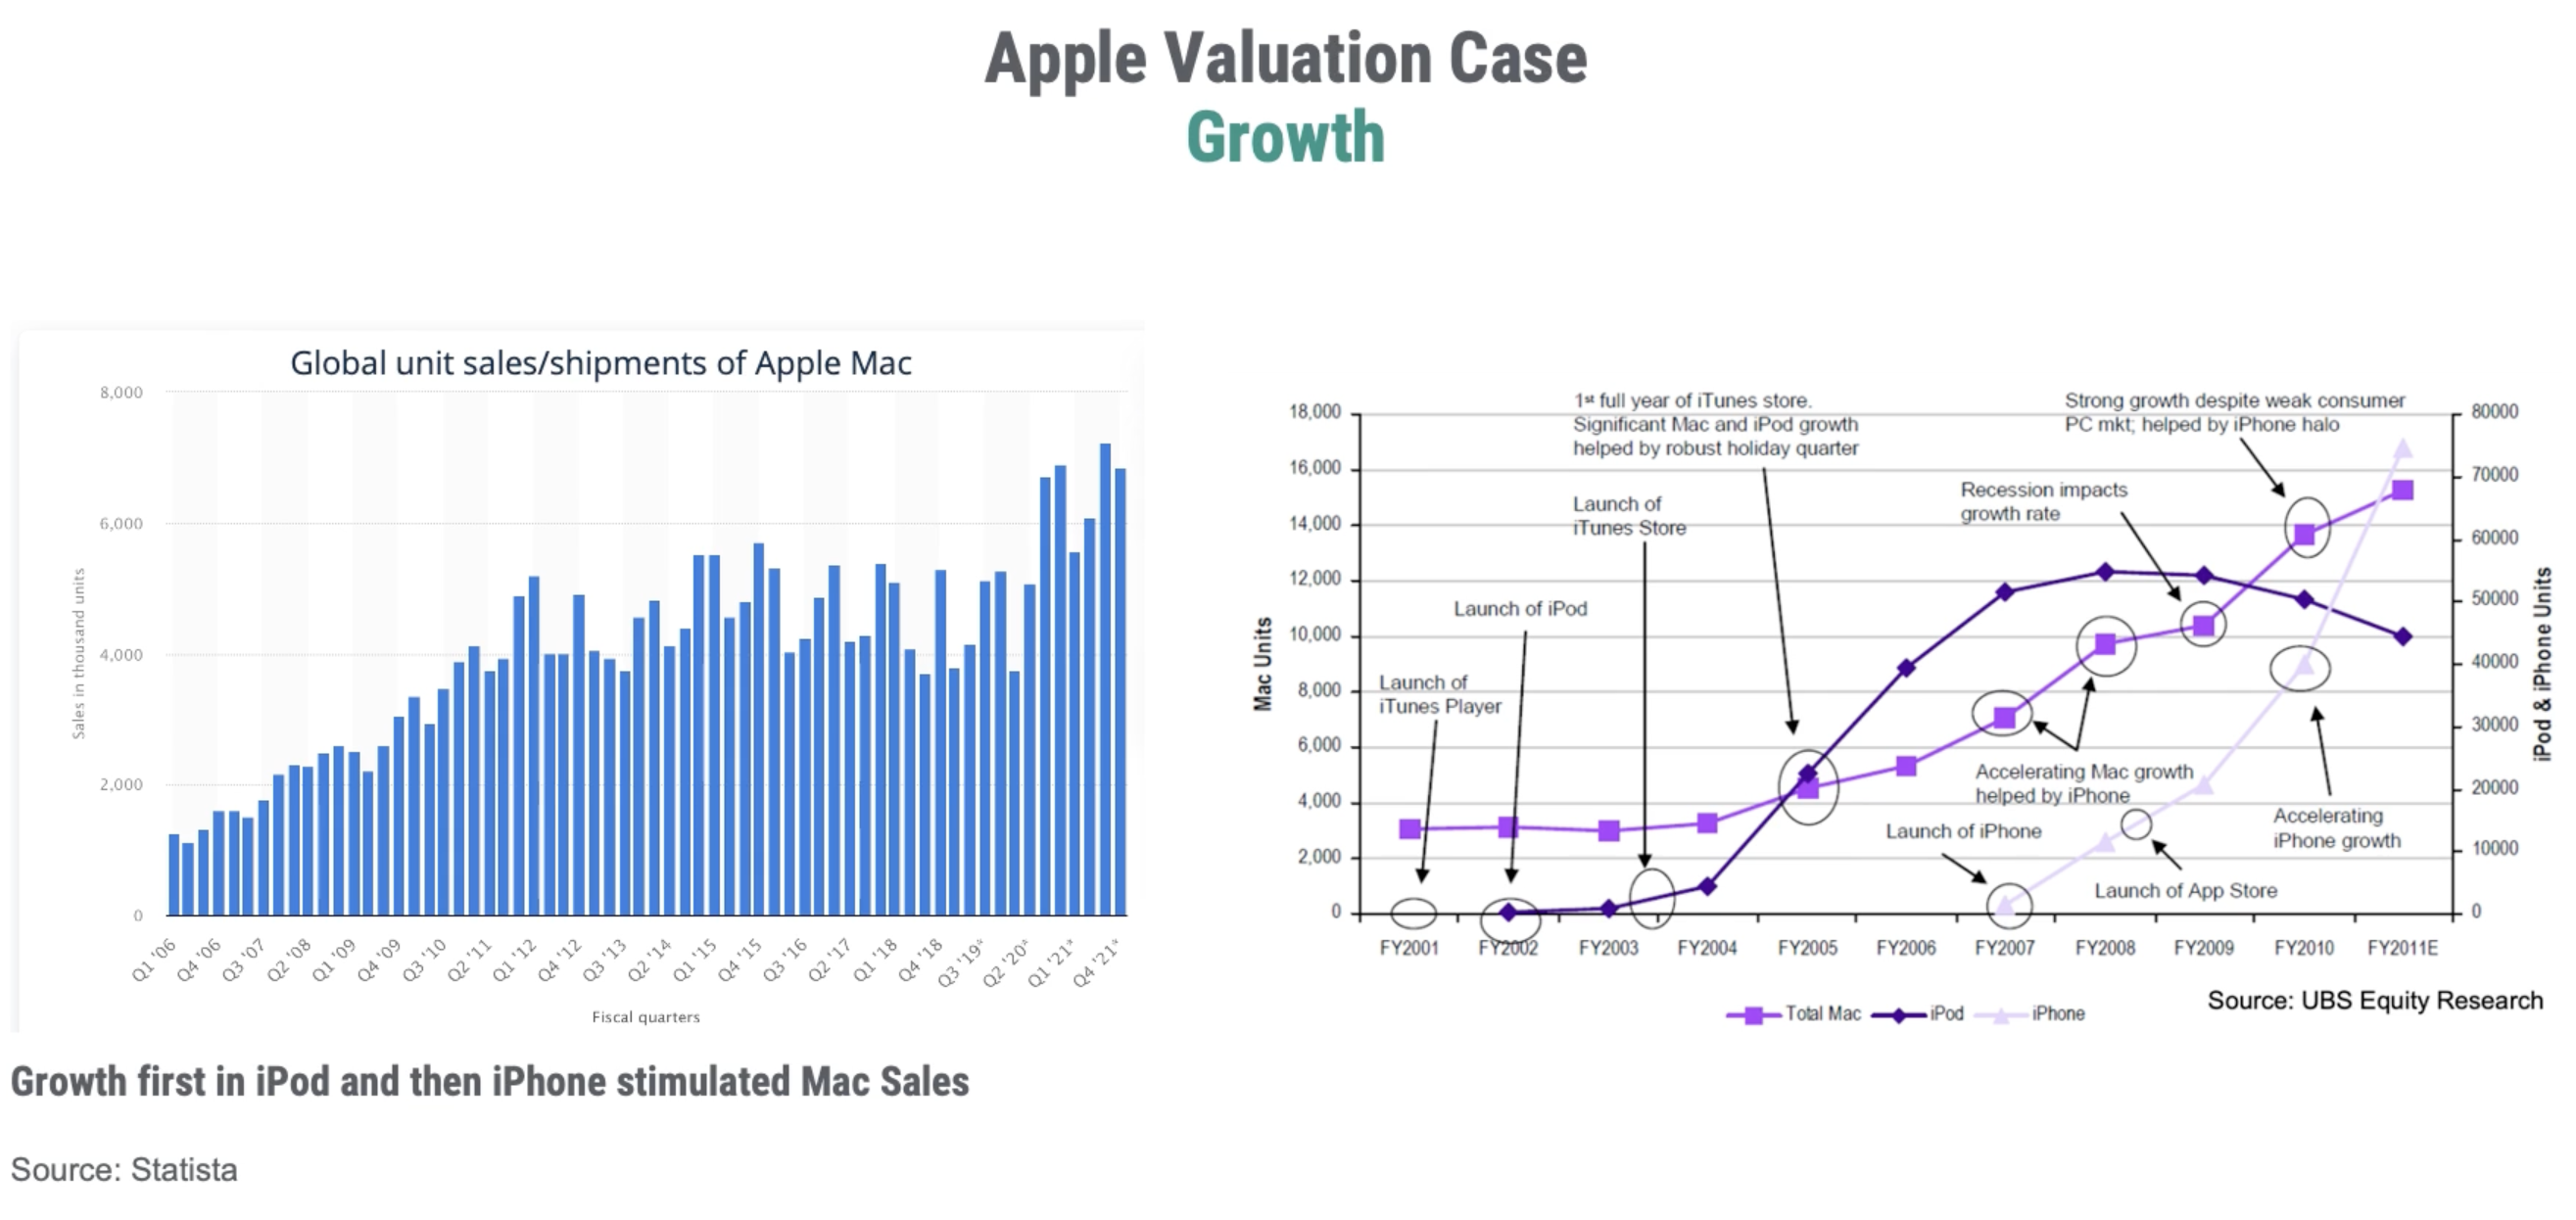
\includegraphics[width=0.5\textwidth]{img/4.4.png}
    \end{figure}
    \begin{figure}[H]
        \centering
        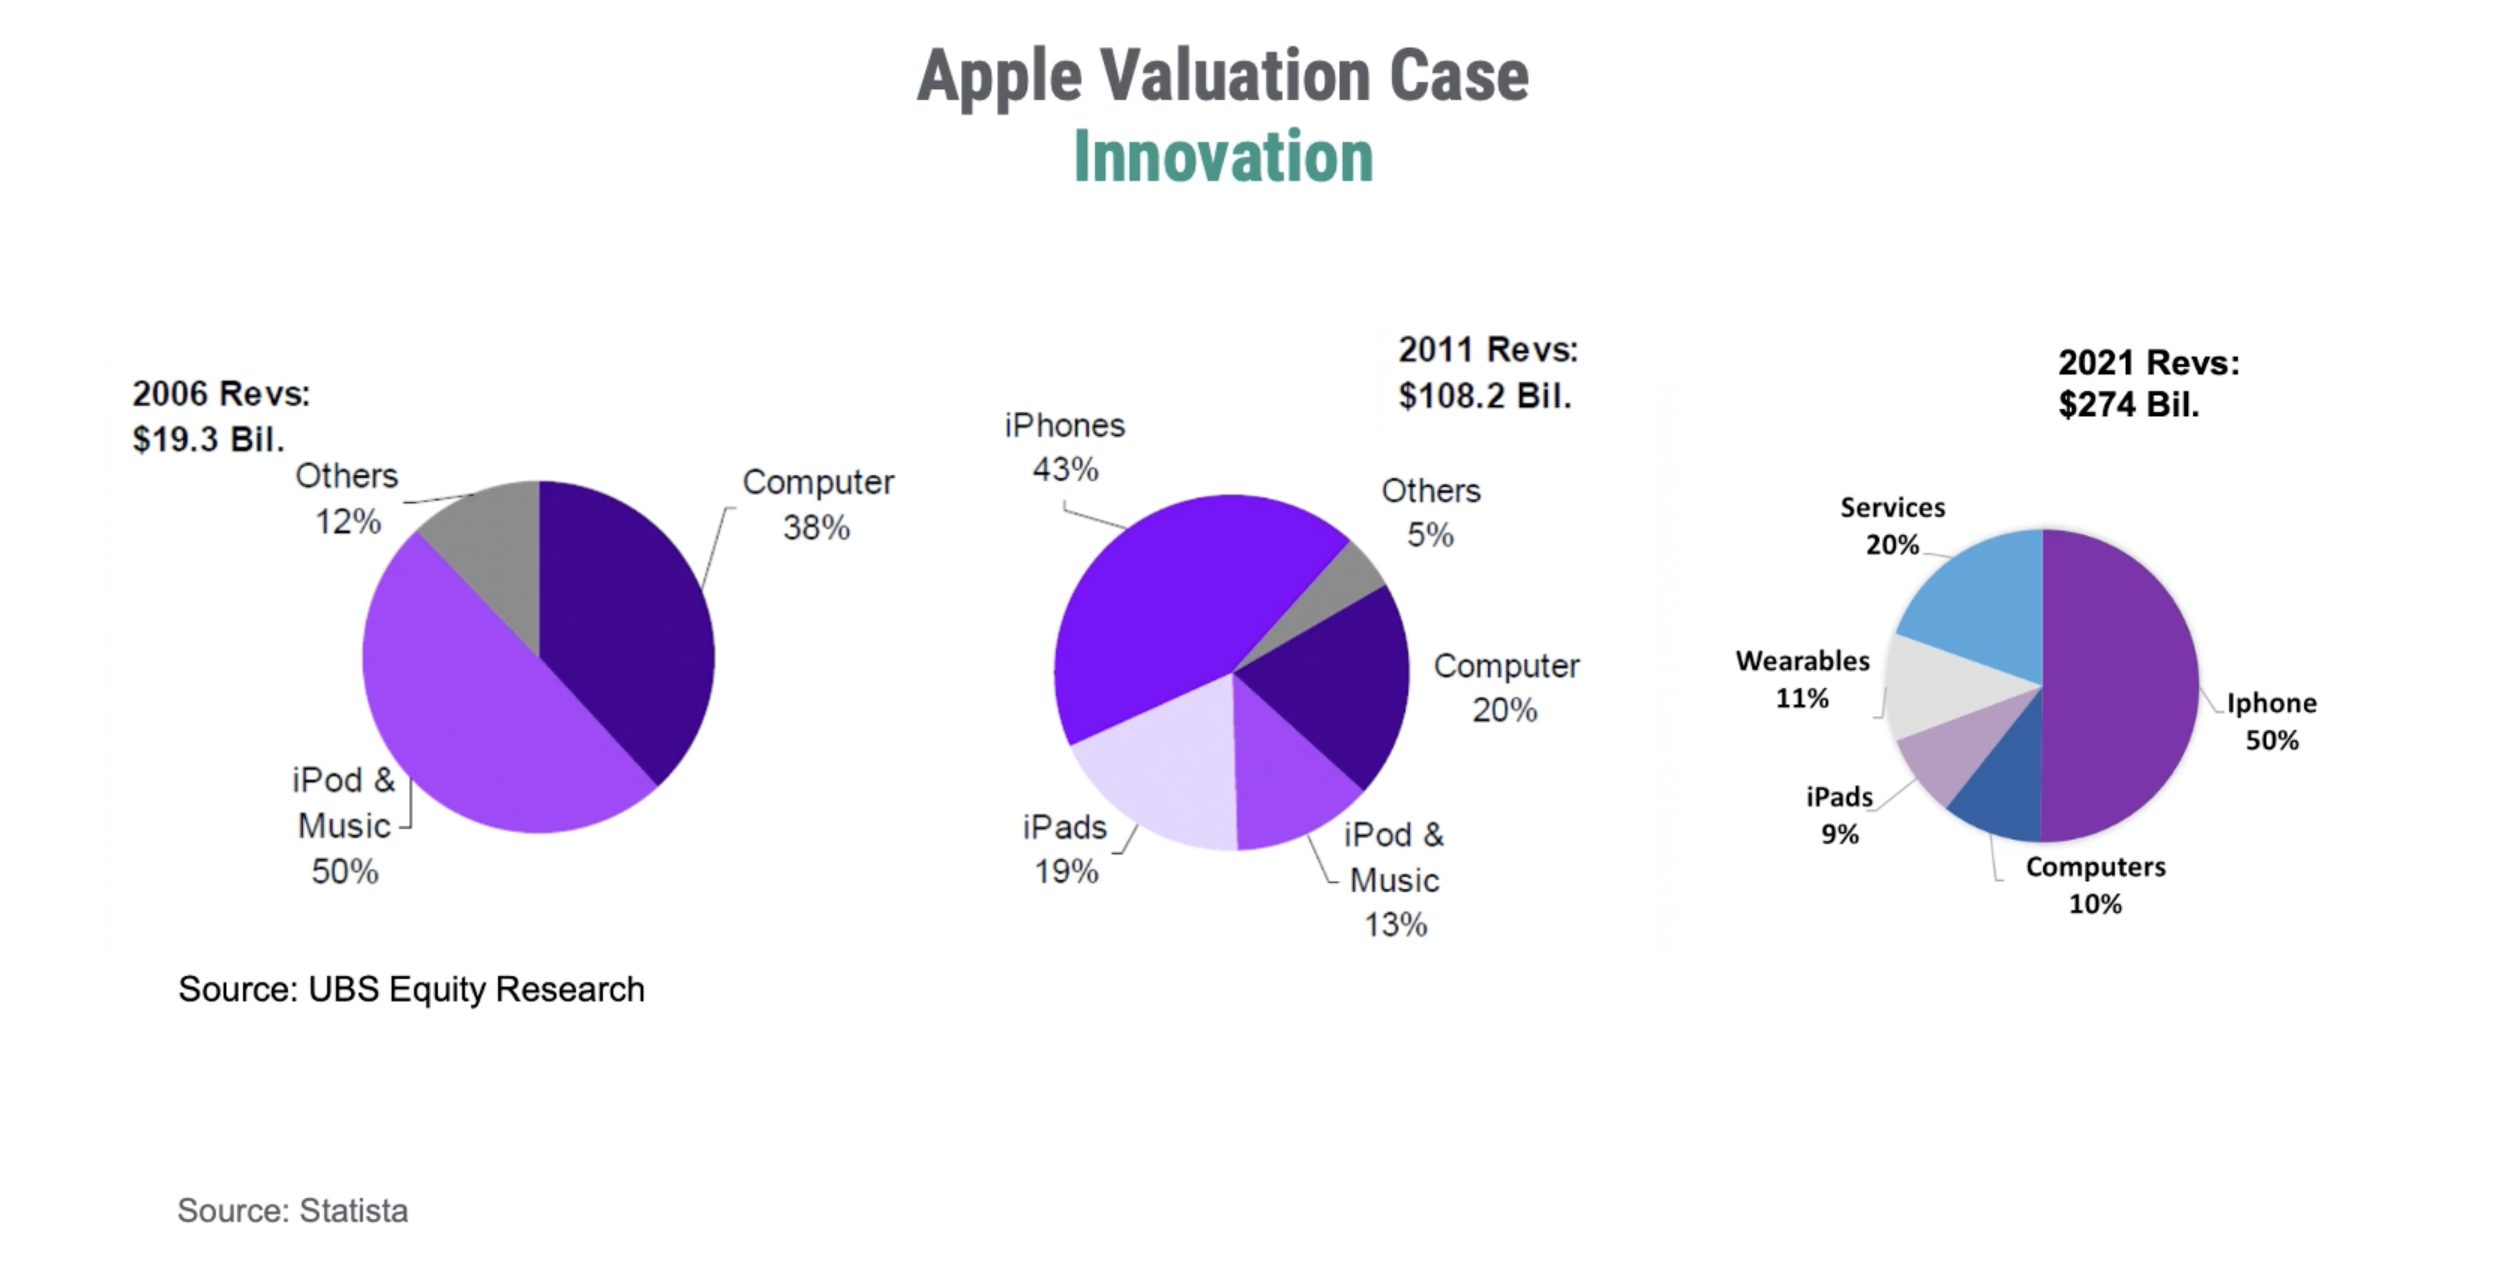
\includegraphics[width=0.5\textwidth]{img/4.5.png}
    \end{figure}
    \item One boost in a product's sales will have a knock-on effect on other products.
    \item It has large profit margins, and a large cash pile.
    \item There have been large return on equity (ROE) and return on assets (ROA) in recent years.
    

\end{itemize}

\begin{table}[ht]
    \centering
    \caption{Apple's Past Performance}
    \label{my-label}
    \tiny
    \begin{tabular}{|l|r|r|r|r|r|r|r|r|r|r|r|}
    \hline
    \textbf{millions of dollars} & \textbf{2012} & \textbf{2013} & \textbf{2014} & \textbf{2015} & \textbf{2016} & \textbf{2017} & \textbf{2018} & \textbf{2019} & \textbf{2020} & \textbf{2021} & \textbf{2022} \\ \hline
    Long term debt               & -             & 16,960        & 28,987        & 53,329        & 75,427        & 97,207        & 93,735        & 91,807        & 98,667        & 109,106       & 148,101       \\ \hline
    Revenue, Total               & 156,508       & 170,910       & 182,795       & 233,715       & 215,639       & 229,234       & 265,595       & 260,174       & 274,515       & 365,817       & 394,328       \\ \hline
    EBIT                         & 55,241        & 48,999        & 52,503        & 71,230        & 60,024        & 61,344        & 70,898        & 63,930        & 66,288        & 108,949       & 119,437       \\ \hline
    Net income                   & 41,733        & 37,037        & 39,510        & 53,394        & 45,687        & 48,351        & 59,531        & 55,256        & 57,411        & 94,680        & 99,803        \\ \hline
    Effective tax rate \%         & 25.2          & 56.2          & 26.1          & 26.4          & 25.6          & 24.6          & 18.3          & 15.9          & 14.4          & 13.3          & 16.4          \\ \hline
    Market capitalisation        & 560,013       & 472,269       & 616,453       & 664,970       & 516,362       & 885,669       & 956,625       & 1,105,307     & 1,850,816     & 2,337,583     & 2,241,050     \\ \hline
    Total dividends paid         & 2,488         & 10,564        & 11,126        & 11,561        & 12,150        & 12,769        & 13,712        & 14,081        & 14,467        & 14,841        & 14,841        \\ \hline
    Repurchase of stock          & 1,226         & 23,942        & 46,158        & 36,752        & 31,292        & 34,774        & 75,265        & 69,714        & 92,527        & 89,402        & -             \\ \hline
    Payout ratio                 & 6.0           & 28.5          & 28.2          & 21.7          & 26.6          & 26.4          & 23.0          & 25.6          & 15.3          & 14.9          & -             \\ \hline
    Total payout ratio           & 8.9           & 93.2          & 145.0         & 90.5          & 95.1          & 98.3          & 149.5         & 151.7         & 113.0         & 104.4         & -             \\ \hline
    Operating margin \%   & 35.3          & 28.7          & 28.7          & 30.5          & 27.8          & 26.8          & 26.7          & 24.6          & 24.1          & 29.8          & 30.3          \\ \hline
Effective tax rate    & 25.2          & 56.2          & 26.1          & 26.4          & 25.6          & 24.6          & 18.3          & 15.9          & 14.4          & 13.3          & 16.4          \\ \hline
CAPX + R\&D rate      & 7.5           & 7.4           & 8.5           & 8.3           & 10.6          & 10.5          & 10.4          & 10.3          & 9.5           & 9.0           & 9.4           \\ \hline
Return on Equity \% (ROE) & 42.8       & 30.6          & 33.6          & 46.2          & 36.9          & 36.9          & 49.4          & 60.9          & 87.9          & \textbf{150.1  }       & \textbf{158.2}         \\ \hline
Return on Assets \% (ROA) & 23.6       & 16.0          & 15.0          & 17.1          & 12.3          & 11.0          & 12.0          & 18.9          & 20.5          & \textbf{31.0}          & \textbf{34.0}          \\ \hline
    \end{tabular}
    \normalsize % Resets the font size to normal for the rest of the text.
    \end{table}
    

Let's determine if Apple is overvalued or undervalued. 

\begin{itemize}
    \item Use average analyst consensus forecasts for the future years 2023-2024 from Reuters
    \item Use analyst forecasts of capital expenditure assume it to grow in line with revenues after 2023
    \item From 2025-2028, assume 6\% growth rate aligning with GDP
    \item 2029 and beyond, a more conservative 4\% growth rate
    \item Assume constant margins of just under 30\%
    \item Assume constant tax rates at 16.5\% of EBIT
    \item Use to calculate free cash flows from 2023-2028
    \item Networking capital investment is assumed to be proportional to revenue
\end{itemize}

Terminal value is estimated using a present value formula, with a discount rate WACC of 10.5\% and a perpetual growth rate of 4\%.

\begin{align}
    TV = \frac{FCF_{2028}}{r_{WACC}-g}\\
    FCF_{2028} = FCF_{2027}*(1+g)
\end{align}

\begin{table}[ht]
    \centering
    \caption{Financial Overview}
    \label{table:financial_overview}
    \small
    \begin{tabular}{|l|r|r|r|r|r|r|r|}
    \hline
    \textbf{}                 & \textbf{2022}     & \textbf{2023}     & \textbf{2024}     & \textbf{2025}     & \textbf{2026}     & \textbf{2027}     & \textbf{2028}     \\ \hline
    Revenue growth rate \%    & -                 & 6.0               & 5.9               & 5.0               & 5.0               & 5.0               & 5.0               \\ \hline
    Earnings growth rate \%   & 9.63\%            & 8.9               & 5.9               & 5.0               & -                 & -                 & -                 \\ \hline
    Revenues                  & 394,328           & 417,988           & 442,649           & 464,781           & 488,020           & 512,421           & 538,043           \\ \hline
    Operating Margin          & 30.3              & 0.31              & 0.28              & 0.30              & 0.30              & 0.30              & 0.30              \\ \hline
    Operating Income (EBIT)   & 119,437           & 130,082           & 137,746           & 139,434           & 146,406           & 153,726           & 161,413           \\ \hline
    Effective tax rate \%     & 13.3              & 17,301            & 18,320            & 18,545            & 19,472            & 20,446            & 21,468            \\ \hline
    NOPAT                     & 103,551.88        & 112,781           & 119,426           & 120,890           & 126,934           & 133,281           & 139,945           \\ \hline
    Depreciation              & 11,104            & 10,780            & 11,899            & 12,494            & 13,119            & 13,775            & 14,464            \\ \hline
    CAPX                      & 10,708            & 10,396            & 11,475            & 12,049            & 12,651            & 13,284            & 13,948            \\ \hline
    Change in NWC             & (27,932)          & (29,607.92)       & (31,354.79)       & (32,922.53)       & (34,568.65)       & (36,297.09)       & (38,111.94)       \\ \hline
    Free Cash Flow (FCF)      & 131,880           & 142,773           & 151,205           & 154,258           & 161,971           & 170,069           & 178,573           \\ \hline
    \end{tabular}
    \normalsize % Resets the font size to normal for the rest of the text.
    \end{table}

    \begin{table}[ht]
        \centering
        \caption{Valuation Summary}
        \label{table:valuation_summary}
        \begin{tabular}{|l|r|}
        \hline
        \textbf{Item}                 & \textbf{Value} ('000s)    \\
        \hline
        EV (sum of PV FCF)            & 2,706,512         \\
        \hline
        Net debt                      & 84,129            \\
        \hline
        Equity                        & 2,622,383         \\
        \hline
        \#Shares Outstanding          & 15,787            \\
        \hline
        Share price                   & 166.11            \\
        \hline
        \end{tabular}
    \end{table}
        

\begin{itemize}
    \item Discounting all the cash flows back to 2022, we get the estimated enterprise value of Apple which is \$2.7 trillion. 
    \item Subtracting net debt of \$84 billion, we get \$2.6 trillion of equity value. 
    \item Divide this by the number of shares outstanding, we get a share price of \$166.11
    \item The DCF is very close to the actual market capitalisation of Apple. This shows that the DCF model is a good way to value companies.
    \item The share price at the end of 2022 was actually \$130, so Apple was undervalued.
    \item These estimates are sensitive as they are based on assumed growth rates
    \item Apple's case illustrates the impact of volatile operating conditions paired with strong cash flow and balance sheet management on share buybacks.
    \item In May 2018, Apple initiated a \$100 billion share repurchase program, significantly increasing their history of substantial buybacks since 2013, influenced by the activist investor Carl Icahn.
    \item By August 2018, Apple's share price hit a record peak. However, on January 4, 2019, amidst heightened market volatility, especially in tech stocks, Apple's shares saw their largest drop since 2013, nearly 10\%, following a forecast of lower quarterly sales largely due to iPhone sales.
    \item Despite these challenges, Apple's business model transformation since 2019 has been fruitful, with the stock yielding annual returns exceeding 25\% from 2019 to 2023.
  \end{itemize}




\section{Comparables}

The \textbf{multiples} or \textbf{comparables} method is another simpler way to value a company. It involves comparing the company to similar companies in the same industry. So we assess whether the company is fairly valued in comparison to others. We compare a valuation ratio or multiple of one company to another, and then assess if the company is fairly valued based on this ratio.\\

While multiples are not as accurate as DCF, they provide a rough indication. Relative value investors use this method to identify undervalued companies.\\

The most used multiple is the price-to-earnings (P/E) ratio. This is the share price divided by the earnings per share. A high P/E ratio shows how much investors are willing to pay for each dollar of earnings. A high P/E ratio
indicates that investors expect higher earnings growth in the future.\\

\begin{equation}
    \text{Basic }P/E = \frac{\text{Share Price}}{\text{Earnings per Share}}
\end{equation}

Analysts use different kinds of ratios.\\

There are trailing earnings, which are the earnings of the past 12 months. There are also forward earnings, which are the estimated earnings for the next 12 months. Sometimes an average of the two are used.\\

The typical consensus is to use the 12-month forward PE ratio.

\begin{equation}
    P/E = \frac{\text{Best estimate of current share price}}{\text{Best estimate of earnings per share expected over 12 months}}
\end{equation}

\begin{itemize}
    \item Calculate the forward P/E ratio for each company in your peer group
    \item Calculate the average P/E ratio for the peer group, this is the industry P/E multiple
    \item Analyse the target company's P/E ratio and compare it to the industry average.
    \item If it is higher, then it is trading at the higher multiple (relatively more expensive than peers)
    \item If it is lower, then it is trading at a lower multiple (relatively cheaper than peers)
    \item A fair value can be estimated by multiplying the industry P/E ration by the earnings per share of the company in question.

\end{itemize}

\begin{equation}
    \text{Fair Value (of the share)} = \text{Industry P/E ratio} \times \text{Earnings per Share of Target Company}
\end{equation}

This is a relatively straightforward model but has its limitations. Its simplicity means it does not account for differences between companies' practices. When a company trades at a different multiple than its peers, it is important to investigate if there are valid reasons for this behaviour.\\

Consider the \textbf{capital structure} of the company such as its equity-to-debt ratio, which can affect the P/E ratio. A company with a higher debt ratio will have a lower P/E ratio.\\

If you have identified an opportunity, use multiple ratios to confirm your findings, e.g. price-to-sales, enterprise-value-to-earnings, price-to-book, etc. Some multiples are more suited for some industries e.g. enterprise-value-to-number-of-subscribers for tech companies.

\section{DCF and pro-forma financial statements}
\href{https://youtu.be/ynlAcc99b4c}{Video link}

\begin{itemize}
    \item A pro-forma is a financial statement that is based on assumptions and projections. It is used to estimate the future financial performance of a company.
    \item It essentially forecasts the next years' performances, up to the terminal value.
    \item The terminal value is the estimated sale price of the company at the final period in the pro-forma.
    \item Take the final sales value, multiply to infer earnings, divide by (r-g) to get the terminal value.
    \item $r$ is usually the interest rate + a few percentage points (risk premium)
    \item Take sales, multiply by sales profitability to get earnings, discount it back
    \item Generally, it's very hard to come up with an accurate pro-forma, let alone predict the future.
\end{itemize}


\chapter{History of Equity Markets}

\section{Introduction}
This chapter explores the relationships between risk and return.\\

The fundamental concept is simple: as investors take on more risk, they expect a higher return. This is the risk-return trade-off.\\


\section{Math for Returns}

\begin{definitionbox}{Purchase of a Share}
    At the end of a period of owning a share, the return consists of two components: the dividend paid out during the period and the value of the share at the end.
    
    The final share price of a stock is the sum of the dividend paid at time $t+1$ and the price of the stock at time $t+1$.
    \begin{equation}
        \text{Share Price} = Div_{t+1} + P_{t+1}
    \end{equation}

    The percentage return can be calculated using the formula:
    \begin{equation}
        R_{t+1} = \frac{Div_{t+1} + P_{t+1} - P_t}{P_t}
    \end{equation}
\end{definitionbox}

\begin{definitionbox}{Dividend Yield and Capital Gain}
    Rearranging the percentage return formula, we can express the return as the sum of the dividend yield and the capital gain:
    \begin{equation}
        R_{t+1} = \frac{Div_{t+1} + P_{t+1} - P_t}{P_t}  = \frac{\overbrace{Div_{t+1}}^{\text{Dividend Yield}}}{P_t} + \frac{\overbrace{P_{t+1} - P_t}^{\text{Capital Gain}}}{P_t}
    \end{equation}

    The dividend yield is the income earned per dollar invested, and the capital gains is the percentage change in the price of the security over the given period, accounting for the growth of the investment's value.
\end{definitionbox}

\begin{definitionbox}{Nominal and real return}
    Used to measure investment performance. The nominal return is the percentage change in the value of an investment over a given period expressed in nominal terms, the currency of the investment.\\
    
    Real return is the nominal return adjusted for inflation. It considers the purchasing power of the investment, accounting for the change in the price level of goods and services.\\

    Inflation can represented with a price index, called the CPI, or consumer price index. It reflects the average price of a basket of goods bought in the economy over a year. Another index, the retail price index (RPI) can be used, which reflects the average price of a typical basket of goods purchased by an average household.\\

    The real return can be calculated using the formula, where $I_t$ is the price index at time $t$:
    \begin{equation}
        R^R_{t+1} = \frac{\frac{Div_{t+1} + P_{t+1}}{I_{t+1}}}{P_t / I_t} - 1
    \end{equation}

    We can rewrite as such, where $h_{t+1}$ is the inflation rate at time $t+1$:
    \begin{equation}
        R^R_{t+1} = (R_{t+1} + 1)(1-h_{t+1}) - 1
    \end{equation}

    We can ignore second order terms, and approximate the real return as:
    \begin{equation}
        R^R_{t+1} \approx R_{t+1} - h_{t+1}
    \end{equation}

\end{definitionbox}


\begin{definitionbox}{The Arithmetic and Geometric Mean}
    The arithmetic mean is the return earned in an average period over the entire investment duration, defined by:

    \begin{equation}
        \bar{R} = \frac{1}{N} \sum_{t=1}^{N} R_t
    \end{equation}



    The geometric mean takes into account the compounding effect, which is more apparent over longer time periods. So it calculates the average compound return per period over the investment duration of $N$ periods, defined by:

    \begin{equation}
        \bar{R}^G = \left( \prod_{t=1}^{N} (1 + R_t) \right)^{\frac{1}{N}} - 1
    \end{equation}


\end{definitionbox}



\begin{examplebox}{Averages Example}
    Consider the following data:
    \begin{itemize}
        \item Year 1: 5\%
        \item Year 2: -3\%
        \item Year 3: 12\%
    \end{itemize}

    The arithmetic average is:
    \begin{equation}
        \bar{R} = \frac{1}{3} (5 - 3 + 12) = 4.67\%
    \end{equation}

    The geometric average is:
    \begin{equation}
        \bar{R}^G = \left( (1 + 0.05)(1 - 0.03)(1 + 0.12) \right)^{\frac{1}{3}} - 1 = 4.67\%
    \end{equation}
\end{examplebox}



\section{Indices and Correlations}

This section gives an exercise to calculate the monthly returns and volatility of three return series, the FTSE 100, the S\&P 500, and the US-10 year bond, followed by calculating correlations.

\begin{sidenotebox}{Volatility}
    The volatility of a return series is a measure of the dispersion of the returns around the mean. It is calculated as the standard deviation of the returns.\\

    The standard deviation is calculated as:
    \begin{equation}
        \sigma = \sqrt{\frac{1}{N} \sum_{t=1}^{N} (R_t - \bar{R})^2}
    \end{equation}
\end{sidenotebox}

\begin{sidenotebox}{Correlation}
    The correlation coefficient measures the strength and direction of a linear relationship between two variables. It ranges from -1 to 1.\\

    A correlation of 1 indicates a perfect positive linear relationship, -1 indicates a perfect negative linear relationship, and 0 indicates no linear relationship.\\

    The correlation coefficient $\rho_{X,Y}$ which represents the correlation between variables $X$ and $Y$, calculated as:
    \begin{equation}
        \rho_{X,Y} = \frac{\cov(X,Y)}{\sigma_X \sigma_Y}
    \end{equation}

    Where $\cov(X,Y)$ is the covariance of $X$ and $Y$, and $\sigma_X$ and $\sigma_Y$ are the standard deviations of $X$ and $Y$ respectively.\\

    The covariance is calculated as:
    \begin{equation}
        \cov(X,Y) = \E[(X - \E[X])(Y - \E[Y])]
    \end{equation}
    This would be calculated as the following summation:
    \begin{equation}
        \cov(X,Y) = \frac{1}{N} \sum_{t=1}^{N} (X_t - \bar{X})(Y_t - \bar{Y})
    \end{equation}

    

    It is quite common to denote correlations between securities using a correlation matrix, where the diagonal elements are 1, and the off-diagonal elements are the correlation coefficients.\\

    Note that $\rho_{X,Y} \equiv \rho_{Y,X}$, so this matrix is symmetric.\\
    
    The correlation matrix is calculated as:
    \begin{equation}
        \mb{C} = \left( \begin{array}{c|ccc}
        & \text{Security 1} & \text{Security 2} & \text{Security 3} \\ \hline
        \text{Security 1} & 1 & \rho_{1,2} & \rho_{1,3} \\
        \text{Security 2} & \rho_{2,1} & 1 & \rho_{2,3} \\
        \text{Security 3} & \rho_{3,1} & \rho_{3,2} & 1 
        \end{array} \right)
    \end{equation}

    An example of what a correlation matrix might look like is:
    \begin{equation}
        \mb{C} = \begin{bmatrix}
            1 & 0.8 & 0.3 \\
            0.8 & 1 & 0.5 \\
            0.3 & 0.5 & 1
        \end{bmatrix}
    \end{equation}

\end{sidenotebox}

\section{Risk and Return}
\begin{itemize}
    \item Generally, higher risk is associated with potential for higher returns, as seen in equities, whereas lower risk investments like bonds offer more modest returns with less volatility.
    \item Historical data highlights that equities typically provide higher average returns but also greater volatility, exposing investors to potential significant losses.
    \item Conversely, less risky assets like government bonds or money market funds yield lower returns but ensure greater stability and are preferred for income preservation.
    \item Analyzing capital market returns shows that stocks exhibit the highest average returns and volatility, while treasuries yield the lowest, reinforcing the positive correlation between risk and return.
\end{itemize}

In Table \ref{tab:risk_return_tradeoff}, we see the risk-return tradeoff for various investments. Note that for the U.S. Treasury Bills, the average return and standard deviation values (bolded) are very low compared to other returns and standard deviations. 
\begin{table}[ht]
    \centering
    \caption{Risk-Return Tradeoff: Geometric Average Returns (1926-2020)}
    \label{tab:risk_return_tradeoff}
    \begin{tabular}{@{}lcc@{}}
    \toprule
    \textbf{Investment} & \textbf{Average Return/Mean Return} & \textbf{Standard Deviation} \\ \midrule
    Small stocks        & 12.52\%                 & 33.16\%                    \\
    S\&P 500            & 10.52\%                 & 19.81\%                    \\
    Corporate bonds     & 7.02\%                  & 8.15\%                     \\
    U.S. Treasury bonds & 5.39\%                  & 8.38\%                     \\
    U.S. Treasury bills & \textbf{3.61\% }        &\textbf{ 3.16\% }           \\
    CPI                 & 3.03\%                  & 1.76\%                     \\ \bottomrule
    \end{tabular}
\end{table}

The relations are better illustrated in a risk-return tradeoff graph, as seen in Figure \ref{fig:risk_return}.

\begin{figure}[H]
    \centering
    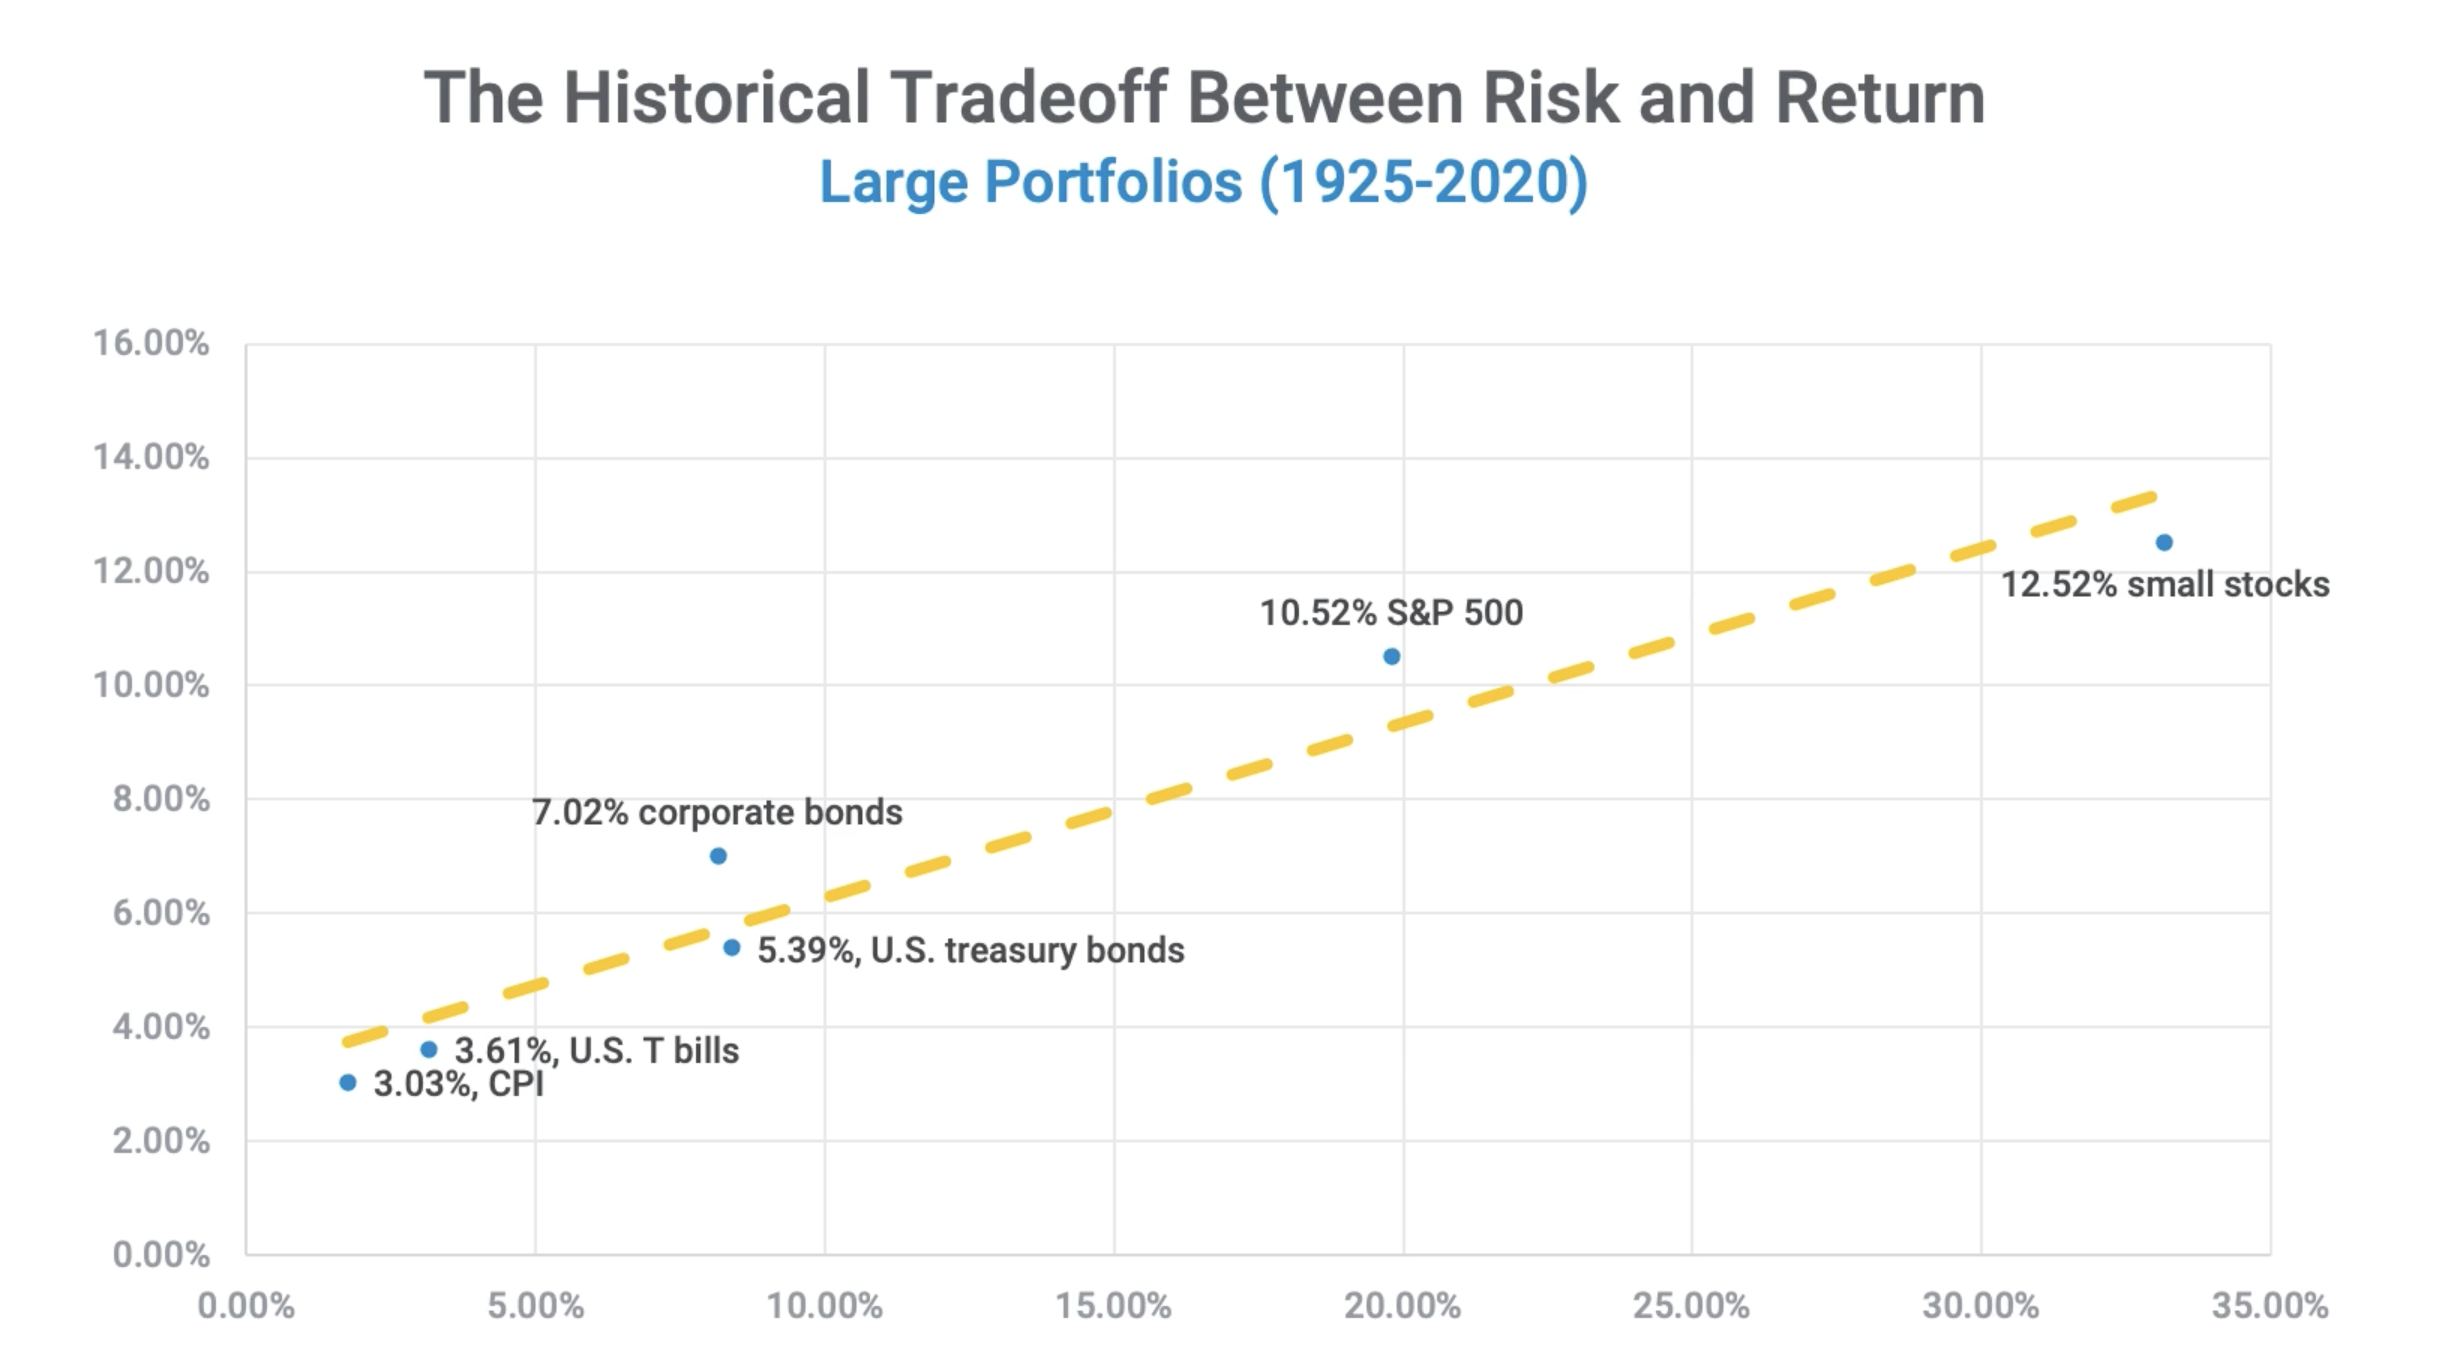
\includegraphics[width=0.8\textwidth]{img/5.4.png}
    \caption{Historical Tradeoff between Risk and Return}
    \label{fig:risk_return}
\end{figure}

\section{Live Tutorial}


\begin{table}[]
    \centering
    \small
    \caption{Summary of Financial Data of a Fictional Company (numbers in '000s)}
    \label{tab:fin_data_live}
    \begin{tabular}{@{}lllllll@{}}
    \toprule
    \textbf{Year (FY end in December)} & \textbf{2023A} & \textbf{2024P} & \textbf{2025P} & \textbf{2026P} & \textbf{2027P} & \textbf{2028P} \\ \midrule
    Revenue Growth Rate                  &           & 15.00\%     & 10.00\%   & 8.00\%        & 6.00\%    & 5.00\%      \\\midrule
    Revenues in \$m                    & 190,000.0      & 218,500.0      & 240,350.0      & 259,578.0      & 275,152.7      & 288,910.3      \\
    EBIT (Operating) margin              & 42.11\%   & 42.50\%     & 42.50\%   & 42.50\%       & 43.50\%   & 42.50\%     \\
    EBIT (Operating income)            & 80,000.0       & 92,862.5       & 102,148.8      & 110,320.7      & 116,939.9      & 122,786.9      \\
    Effective Tax Rate                   & 16.50\%   & 16.50\%     & 16.50\%   & 16.50\%       & 16.50\%   & 16.50\%     \\\midrule
    EBIT(1-t)                            & 66,800.0  & 77,540.2    & 85,294.2  & 92,117.7      & 97,644.8  & 102,527.0   \\
    - Capex                              & -24,000.0 & -27,600.0   & -30,360.0 & -32,788.8     & -34,756.1 & -36,493.9   \\
    + Depreciation                       & 14,000.0  & 16,100.0    & 17,710.0  & 19,126.8      & 20,274.4  & 21,288.1    \\
    \textbf{- Change in NWC*}            &           & -3,675.0    & -2,817.5  & -2,479.4      & -2,008.3  & -1,774.0    \\\midrule[2pt]
    FCFF                                 &           & 62,365.2    & 69,826.7  & 75,976.3      & 81,154.8  & 85,547.2    \\
    - FCFF for 01/2024                   &           & -5,197.1    &           &               &           &             \\
    FCFF excluding 01/2024               &           & 57,168.1    & 69,826.7  & 75,976.3      & 81,154.8  & 85,547.2    \\\midrule[2pt]
    \textbf{Cost of capital (WACC) **}              &           & 10.92\%     & 10.92\%   & 10.92\%       & 10.92\%   & 10.92\%     \\\midrule[2pt]
    Number of years from 'NOW'           &           & 0.92        & 1.92      & 2.92          & 3.92      & 4.92        \\
    Cumulated discount factor            &           & 0.91        & 0.82      & 0.74          & 0.67      & 0.60        \\
    PV(FCFF)                             &           & 51,989.0    & 57,251.6  & 56,163.4      & 54,087.5  & 51,404.1    \\ \midrule
    Terminal Value (TV)                  &           &             &           &               &           & 1,518,507.1 \\
    PV (TV)                              &           & 912,448.5   &           &               &           &             \\
    Enterprise Value = Sum of PV         &           & 1,183,344.1 &           & 77\% TV as EV &           &             \\
    - Net Debt                           &           & -50,000.0   &           &               &           &             \\
    Value of Equity                      &           & 1,133,344.1 &           &               &           &             \\
    Number of Shares in millions         &           & 7,500.0     &           &               &           &             \\
    Implied Share Price                  &           & \textbf{151.11  }    &           &               &           &             \\
    Current Share Price as of 12/02/2024 &           & 200         &           &               &           &             \\
    Overrvalued by                       &           & \textbf{32.35\% }    &           &               &           &             \\ \bottomrule
    \end{tabular}
    \end{table}



    \begin{table}[ht]
        \centering
        \caption{Summary of Changes in Net Working Capital* (numbers in '000s)}
        \label{tab:nwc_summary}
        \begin{tabular}{@{}lrrrrrr@{}}
        \toprule
        \textbf{Description} & \textbf{2023A} & \textbf{2024P} & \textbf{2025P} & \textbf{2026P} & \textbf{2027P} & \textbf{2028P} \\
        \midrule
        A/R               & 40,000.0 &       &       &       &       &       \\
        Inventory         & 3,500.0  &       &       &       &       &       \\
        A/P               & -19,000.0&       &       &       &       &       \\
        \midrule
        NWC               & 24,500.0 & 28,175.0 & 30,992.5 & 33,471.9 & 35,480.2 & 37,254.2 \\
        $\Delta$ in NWC   & 3,675.0  & 2,817.5 & 2,479.4 & 2,008.3  & 1,774.0  &       \\
        \bottomrule
        \end{tabular}
    \end{table}

\begin{table}[ht]
    \centering
    \caption{WACC ** (numbers in '000s)}
    \label{tab:wacc}
    \begin{tabular}{@{}lc@{}}
    \toprule
    \textbf{Metric}                     & \textbf{Value}    \\
    \midrule
    Cost of Debt                        & 5.00\%            \\
    Effective Tax Rate                  & 16.50\%           \\
    Total Debt                          & \$55,000.00       \\
    Cash \& Short-term Inv.             & \$5,000.00        \\
    Net Debt                            & \$50,000.00       \\
    After Tax Cost of Debt              & 4.18\%            \\
    Risk Free Rate                      & 4.00\%            \\
    Beta                                & 1.02              \\
    Market Risk Premium                 & 7.00\%            \\
    Cost of Equity                      & 11.14\%           \\
    MV of Equity on 12/02/2024          & \$1,500,000.00    \\
    D/V                                 & 3.2\%             \\
    E/V                                 & 96.8\%            \\
    WACC                                & 10.92\%           \\
    \bottomrule
    \end{tabular}
\end{table}

\begin{itemize}
    \item Whole point of the DCF: determine if the company is undervalued or overvalued. We only intend to buy underpriced stocks.
    \begin{itemize}
        \item Some questions to ask:
        \item How is it doing in comparison to competitors?
        \item Cross-selling opportunities? A cross-selling opportunity is when a company sells a different product or service to an existing customer.
        \item Any planned mergers or acquisitions?
    \end{itemize}
    \item Start with the income statement.
    \item Then make assumptions on:
    \item \textbf{Revenue Growth: } (Table \ref{tab:fin_data_live})
        \begin{itemize}
            \item There was double-digit growth forecasted from 2023-2025, but it cannot be sustained forever. DCF cannot forecast an infinite number of cash flows forever. So let 2028 be the terminal year, and it will cap at a 5\% growth rate.
            \item This capped growth rate usually has an upper limit equal to the GDP growth rate of the company's country. This could differ if the company is a multinational one.
        \end{itemize}
    \item \textbf{Operating Margins: } (Table \ref{tab:fin_data_live})
        \begin{itemize}
            \item After determining the revenue growth assumptions, next estimate the \textbf{operating margins}.
            \item  There are different margins, such as the profit margin, EBIT, etc.
            \item Currently for 2023 it is \textbf{42.11\%}. Assume it has no plans for expansion, so the margin will remain constant.
            \item Let's also assume this fictional is a service company, so it also does not have much room for improvement in margins.
            \item When determining this, it is important to look into the company's expansion strategy.
        \end{itemize}
    \item \textbf{EBIT or Operating Income: } (Table \ref{tab:fin_data_live})
    \begin{itemize}
        \item Assume tax rate remains constant at 16.5\%. Using the marginal or statutory tax rates (values which are provided by tax authorities) are generally higher, so companies are highly incentivised to not pay them and can avoid paying all of the taxes, by using strategies like tax havens, depreciation of assets as a non-cash expense, tax credits, deducting interest expenses from debt financing (companies are not taxed on debt).
        \item We've assumed it to remain constant at 16.5\%. 
        \item Also, when decided tax rates, do not account for outliers (spikes) as they are likely one-time events.
        \item \textbf{EBIT(1-t)} is also known as NOPAT, net operating profit after tax.  
    \end{itemize}
    \item \textbf{Other Assumptions: } (Table \ref{tab:fin_data_live})    
    \begin{itemize}
            \item Assume \textbf{CAPEX} grows with revenue (likely if the company is at maximum capacity, and likes to expand). However, if you're aware a company is cost-cutting, then CAPEX can decrease.
            \item \textbf{Depreciation} is also assumed to increase with revenue (because there is more investment in assets like machinery, buildings, etc.)
            \item $CAPEX - Depreciation = Net \ Investment$ and this value always must be positive.
        \end{itemize}
    \item \textbf{Net Working Capital} (Table \ref{tab:nwc_summary})    
    \begin{itemize}
        \item $NWC = Current \ Operating \ Assets - Current \ Operating \ Liabilities $
        \item We had \$24.5M in 2023, and can assume if the business likes to expand, it will invest more in working capital.
        \item Assume it increases with revenue, so it remains the same proportion of revenue (in this example, 12.89\%).
    \end{itemize}
    \item Note that the FCFF in 2024 has its first month deducted from it, as we assume it's January, and the company's end of the financial year ends in December.
    \item \textbf{WACC} (Table \ref{tab:wacc})
    \begin{itemize}
        \item $WACC = (D/V)*\text{After-tax Cost of Debt} + (E/V)*\text{Cost of Equity}$ where $D/V$ is the debt to value ratio, and $E/V$ is the equity to value ratio.
    \end{itemize}
\end{itemize}

To summarise, once we have completed the assumptions, we are able to work out the present value of forecasted cash flows. When adding in the terminal value, we can calculate the enterprise value. Subtracting the net debt, we can calculate the equity value. Dividing this by the number of shares outstanding, we can calculate the share price. In our example, we believe the share price is overvalued by 32.35\%.

\chapter{Portfolio Allocation}
\section{Introduction}

In the past chapter, we looked at simple models of the risk-return trade-off, however models can be more complex for a single security. This chapter goes through the CAPM or Capital Asset Pricing Model, which is a model that describes the relationship between risk and expected return.

\begin{definitionbox}{Definition of Portfolio Allocation}
    Portfolio allocation refers to the distribution of an individual's investment across different asset classes, such as stocks, bonds, and real estate, with the aim of maximising returns while minimising risk.
\end{definitionbox}

\section{Portfolio Theory}
When calculating the return and volatility of a two-stock portfolio, we consider the weighted average of the returns and variances based on the allocation of the two stocks, where $x_i$ is the weight of the portfolio invested in asset $i$ and $R_i$ is the return of asset $i$. Note that the weights $x_A, x_b$ must sum to 1.

\begin{equation}
    R_p = x_AR_A + x_BR_B
\end{equation}

Denote the volatilities of the two assets as $\sigma_A, \sigma_B$ and the correlation between the two assets as $\rho_{AB}$. The volatility of the portfolio is given by:

\begin{equation}
    \sigma_p = \sqrt{\underbrace{x_A^2\sigma_A^2}_{\text{A's individual contribution to vol}} + \underbrace{x_B^2\sigma_B^2}_{\text{B's individual contribution to vol}} + \underbrace{2x_Ax_B\sigma_A\sigma_B\rho_{AB}}_{\text{Covariance between A and B}}}
\end{equation}

Changing portfolio weights can change the risk-return profile of the portfolio. 

Assume we have a portfolio of Coca-Cola and Intel.

\begin{table}[ht]
    \centering
    \caption{Expected Returns and Volatility for Intel and Coca-Cola}
    \label{tab:intel-coke}
    \begin{tabular}{@{}lcc@{}}
    \toprule
    \textbf{Company} & \textbf{E(R)} & \textbf{Vol} \\
    \midrule
    Intel    & 26\% & 50\% \\
    Coca-Cola & 6\%  & 25\% \\
    \midrule
    \multicolumn{3}{c}{Correlation = 0} \\
    \bottomrule
    \end{tabular}
 \end{table}

Table \ref{tab:intel-coke} shows possible weight allocations for Coca-Cola and intel. Note that the variance of the portfolio is not a weighted average of the variances of the two stocks, because of the added covariance term. Since these patterns may not be intuitive, it is best to visualise portfolios with a graph to show the \textbf{efficient frontier}


\begin{table}[ht]
    \centering
    \caption{Portfolio Expected Return and Standard Deviation}
    \begin{tabular}{@{}cccc@{}}
    \toprule
    \textbf{Xi} & \textbf{Xc} & \textbf{E(Rp)} & \textbf{SD(Rp)} \\ 
    \midrule
    1    & 0    & 26.00\% & 50.00\% \\
    0.98 & 0.02 & 25.60\% & 49.00\% \\
    0.88 & 0.12 & 23.60\% & 44.10\% \\
    0.78 & 0.22 & 21.60\% & 39.39\% \\
    0.68 & 0.32 & 19.60\% & 34.93\% \\
    0.58 & 0.42 & 17.60\% & 30.84\% \\
    0.48 & 0.52 & 15.60\% & 27.29\% \\
    0.38 & 0.62 & 13.60\% & 24.52\% \\
    0.28 & 0.72 & 11.60\% & 22.80\% \\
    0.18 & 0.82 & 9.60\%  & 22.39\% \\
    0.08 & 0.92 & 7.60\%  & 23.35\% \\
    0    & 1    & 6.00\%  & 25.00\% \\
    \bottomrule
    \end{tabular}
    \end{table}



Diversification can reduce some risk without compromising on returns (making an efficient portfolio). 

\begin{figure}[H]
    \centering
    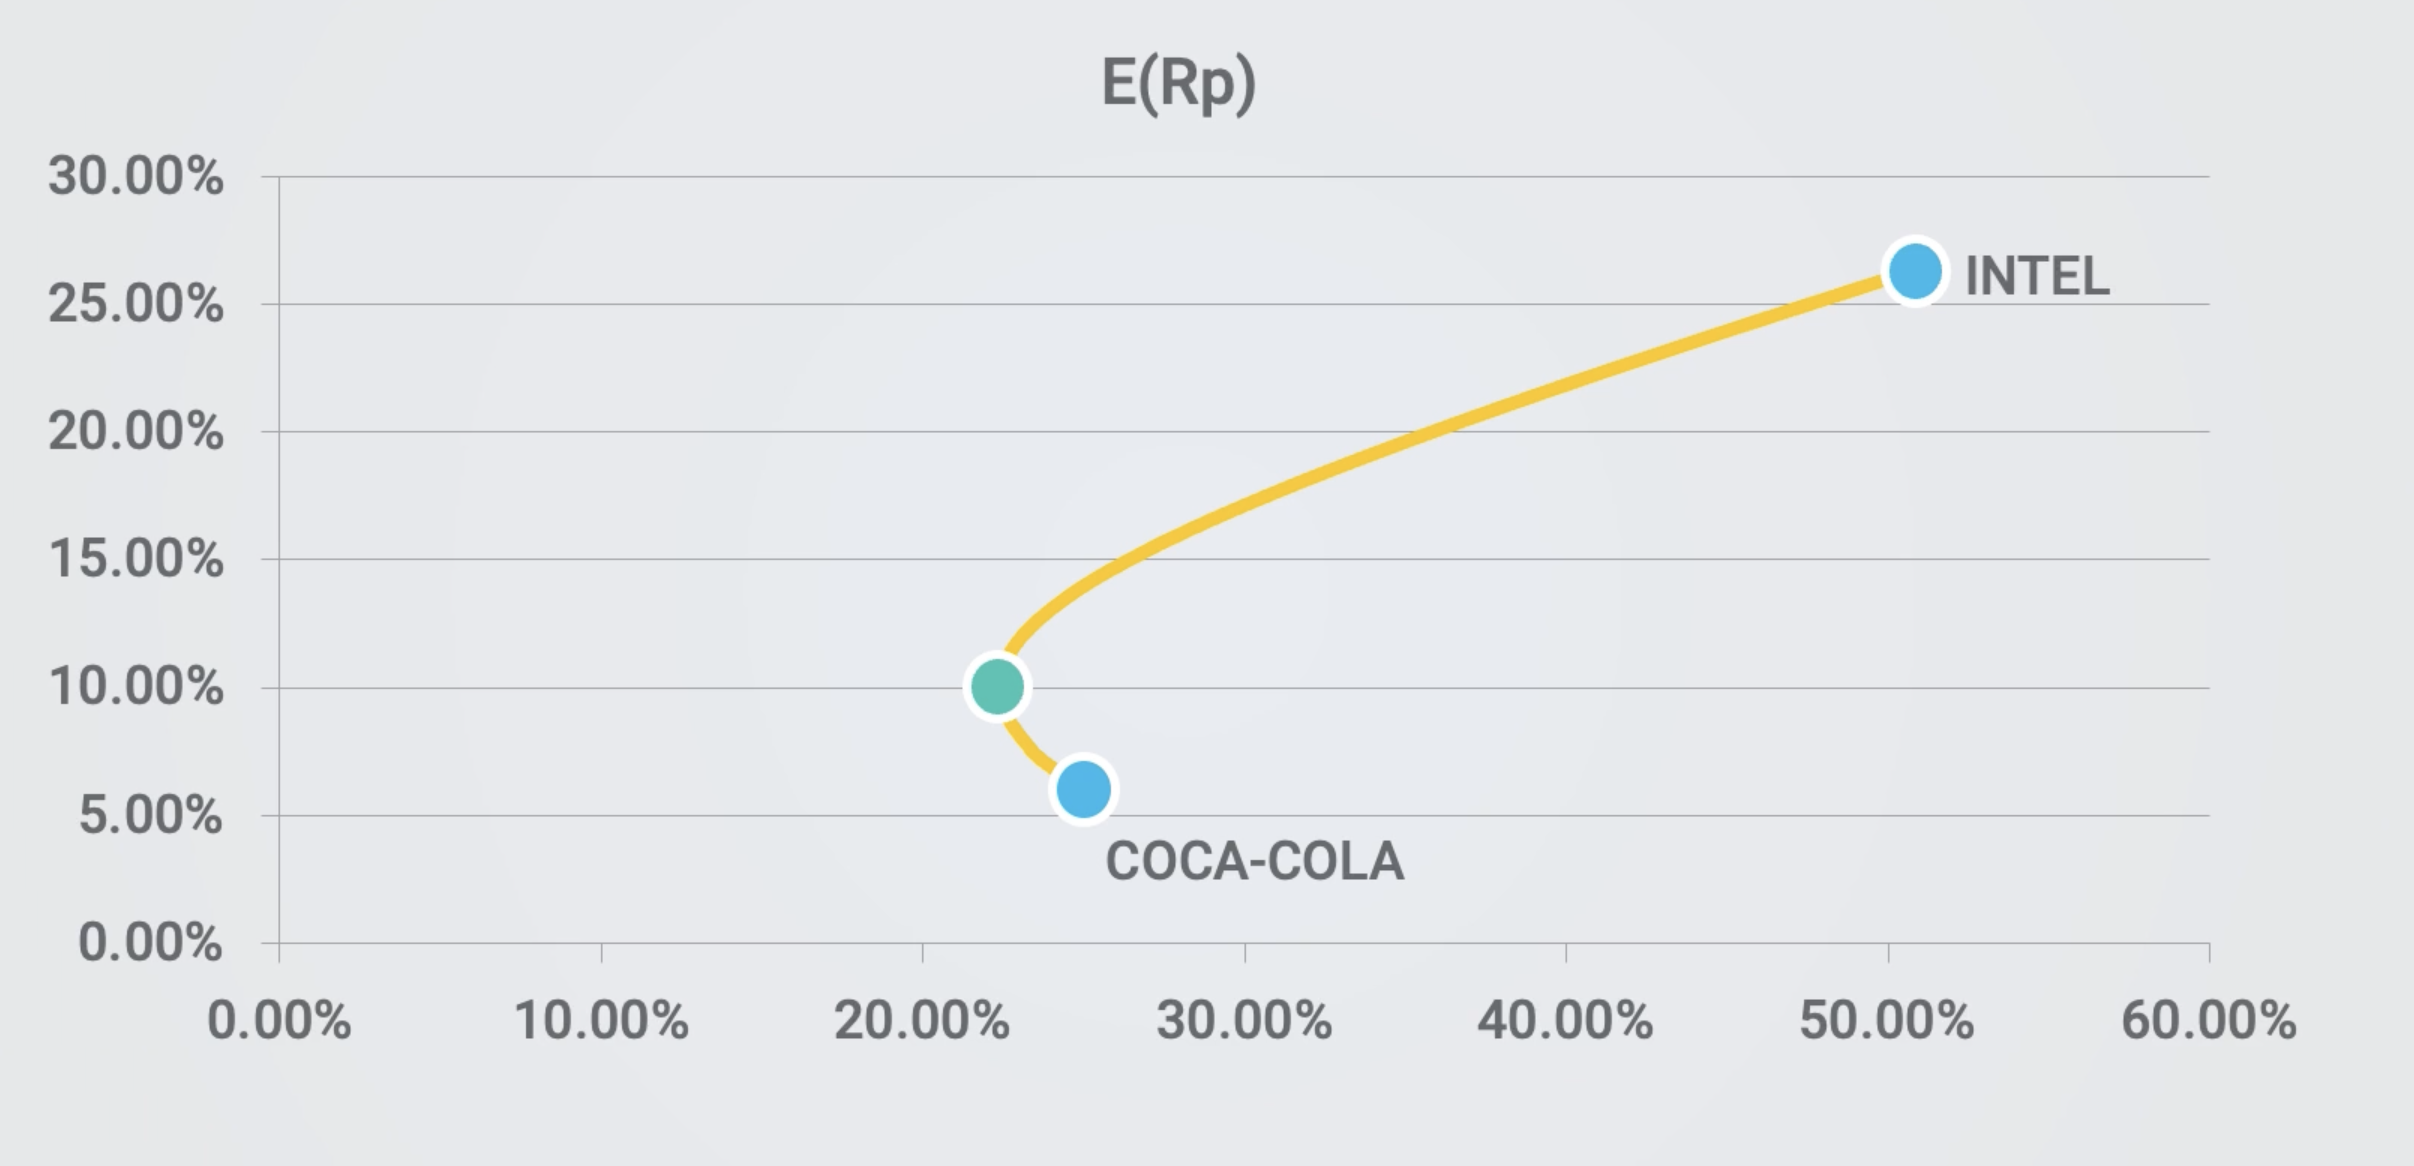
\includegraphics[width=0.8\textwidth]{img/6.2.1.png}
    \caption{Efficient Frontier}
    \label{fig:efficient_frontier}    
\end{figure}

Notice that COCA-COLA by itself has a lower return and lower risk than if it was slightly supplemented by Intel, where risk is reduced to a minimum but returns are slightly higher, thus an efficient portfolio. An efficient portfolio is one that has the highest return for a given level of risk, or the lowest risk for a given level of return.\\

Return correlation is a measure of how two assets move together. A correlation of 1 means that the two assets move in the same direction, while a correlation of -1 means that the two assets move in opposite directions. A correlation of 0 means that the two assets are independent of each other.\\

\begin{figure}[H]
    \centering
    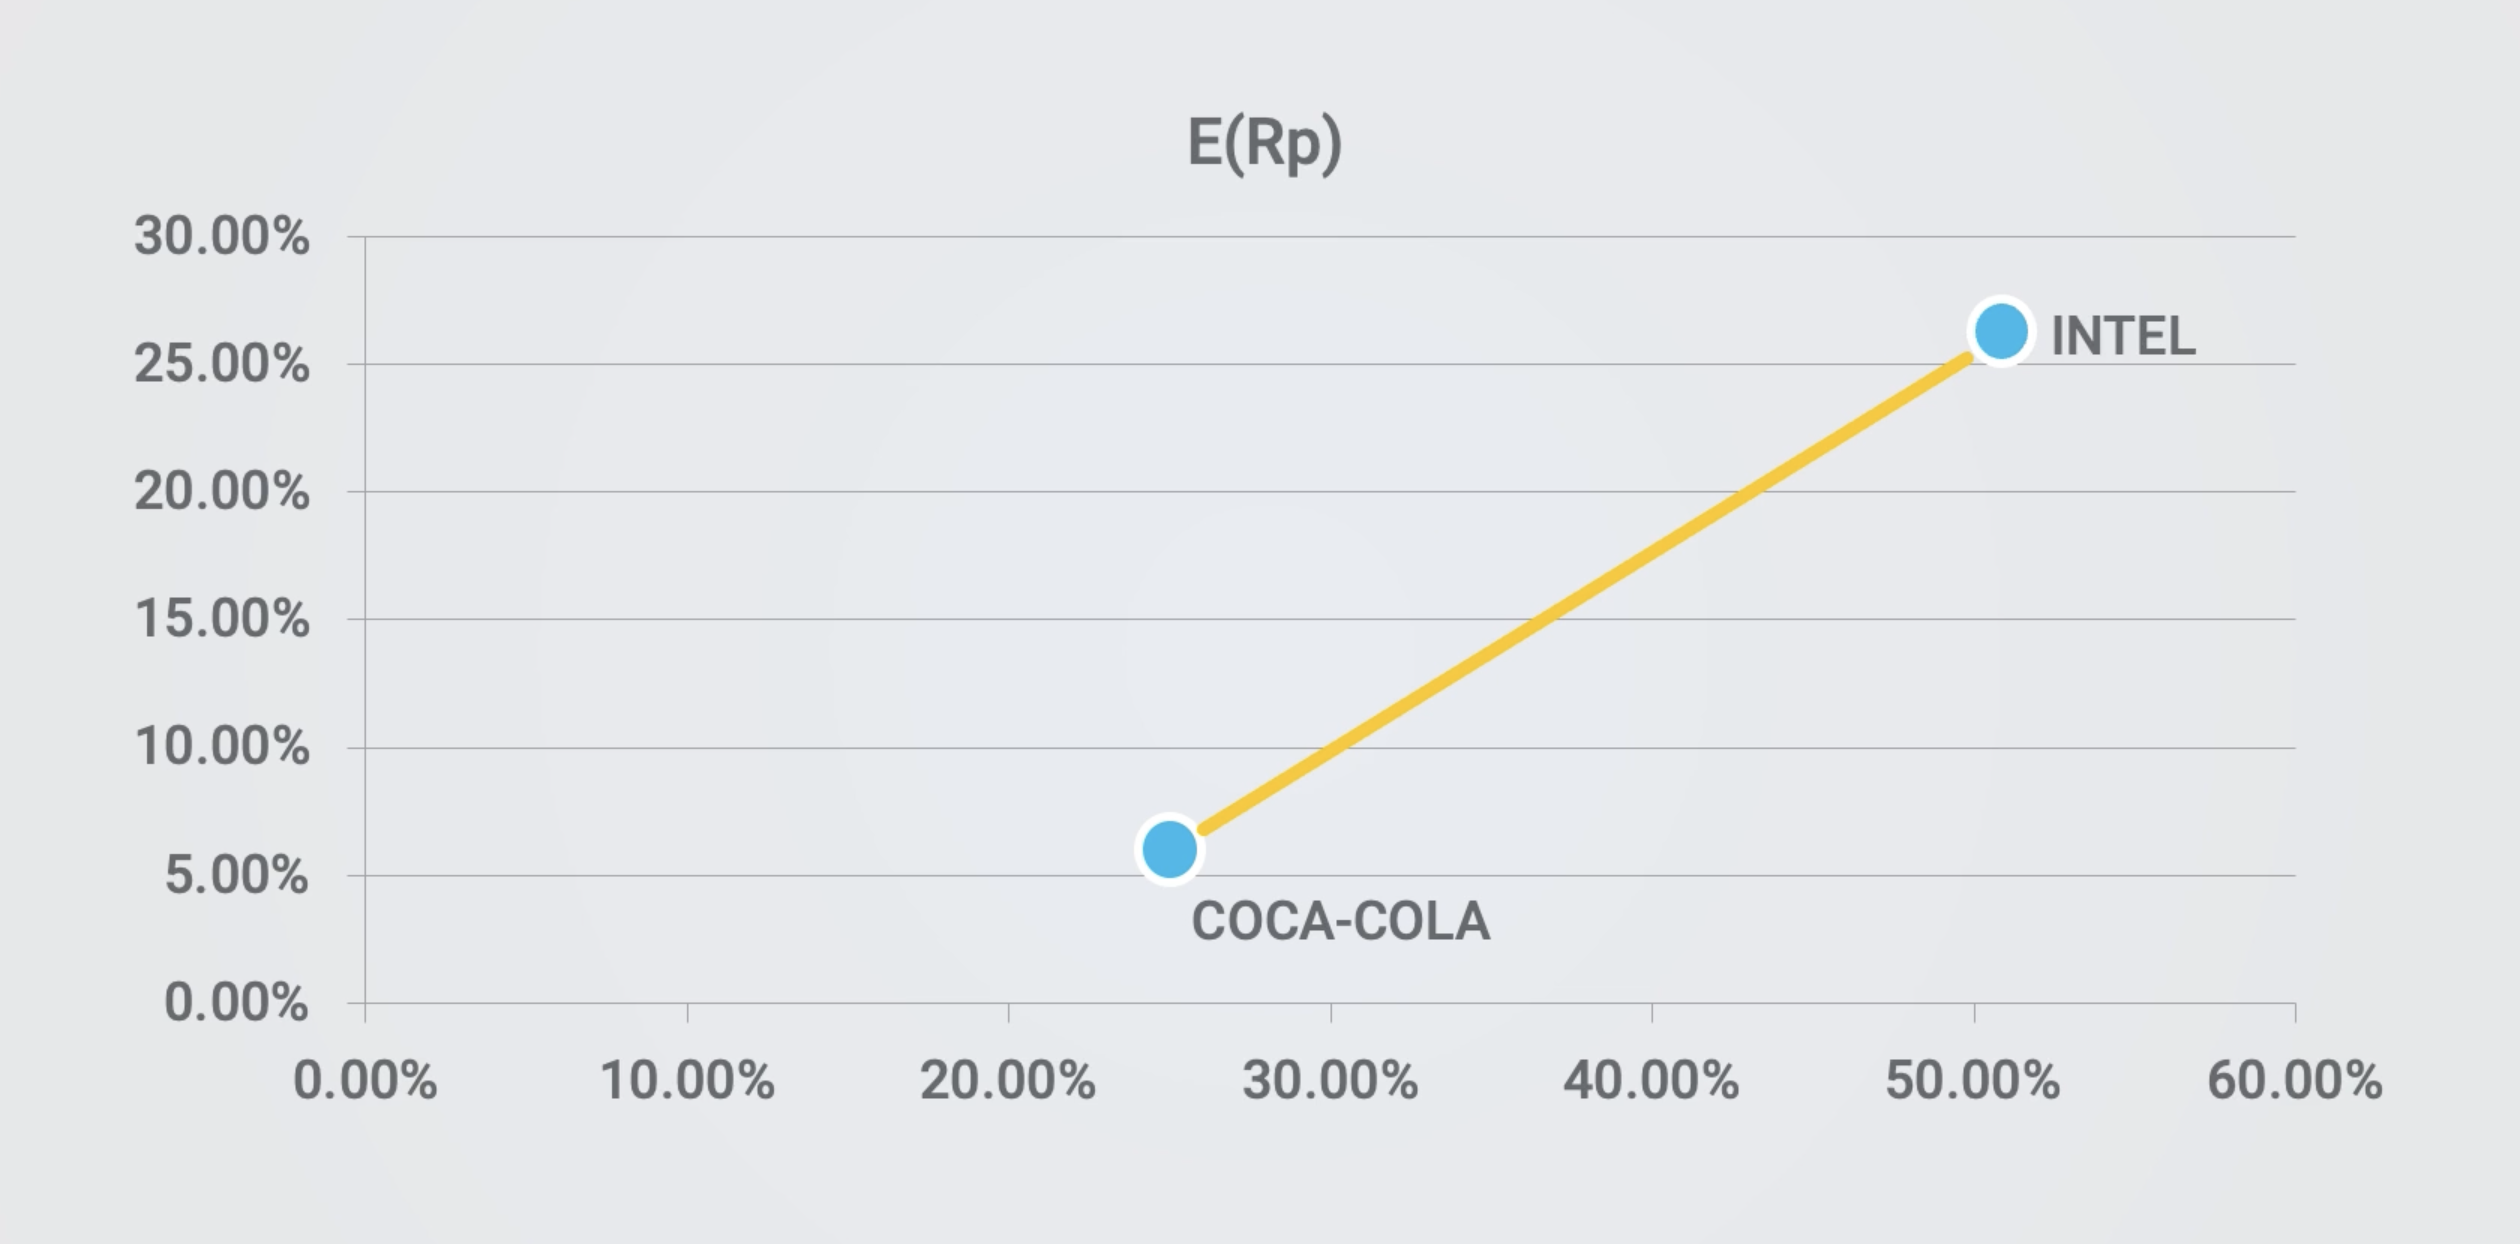
\includegraphics[width=0.8\textwidth]{img/6.2.2.png}
    \caption{Efficient Frontier if Intel and Coca-Cola have a correlation of 1}
    \label{fig:efficient_frontier_2}    
\end{figure}

If Intel and Coca-Cola have a correlation of 1, the efficient frontier will be a straight line, as the two assets move in the same direction. This means that there is no diversification benefit from holding both assets.\\

\begin{figure}[H]
    \centering
    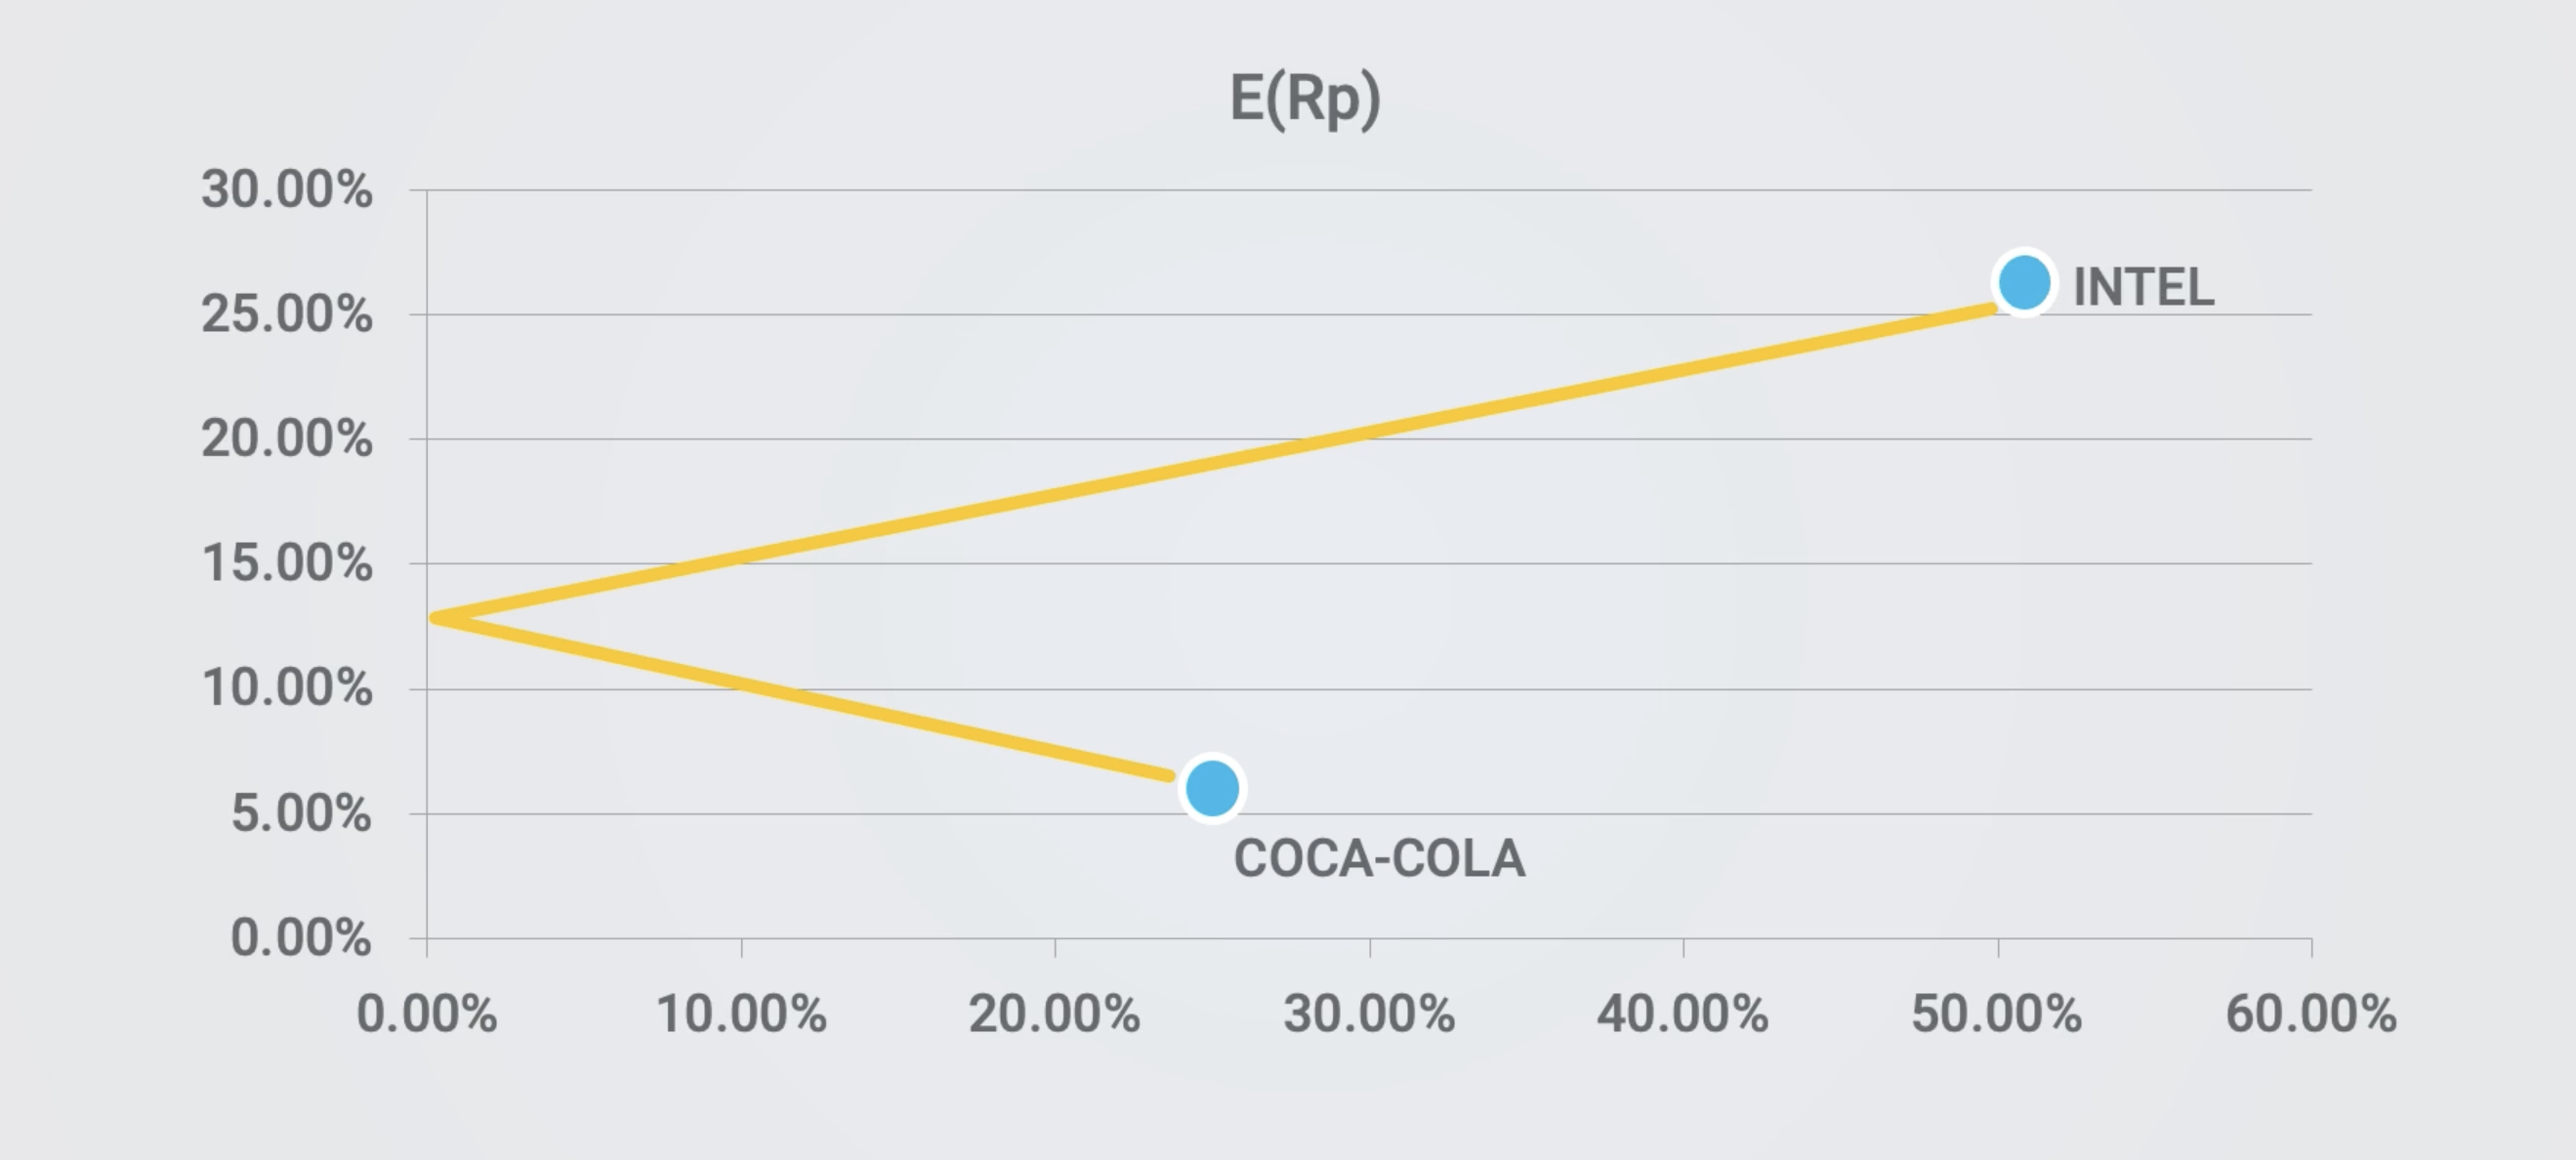
\includegraphics[width=0.8\textwidth]{img/6.2.3.png}
    \caption{Efficient Frontier if Intel and Coca-Cola have a correlation of -1}
    \label{fig:efficient_frontier_3}    
\end{figure}

If Intel and Coca-Cola have a correlation of -1, the efficient frontier will be a two-piece straight line, as the two assets move in opposite directions, so we can achieve a much lower risk for a given level of return.\\





\section{Principle of Diversification}

There are two components of total risk that investors face when investing:

\begin{enumerate}
    \item \textbf{Systematic Risk:} This is the risk that is inherent in the market that affects all companies, and cannot be diversified away. It is also known as market risk or non-diversifiable risk. Examples include interest rate risk, inflation risk, and political risk.
    
    \item \textbf{Idiosyncratic Risk:} This is the risk that is specific to a particular company or industry and can be diversified away. It is also known as idiosyncratic risk or diversifiable risk. It arises from factors that are specific to an individual asset or company, such as management decisions, competitive dynamics, operational issues, regulatory changes or even random events.  Examples include business risk, financial risk, and liquidity risk.
\end{enumerate}

In some asset pricing models like the CAPM, investors are compensated for taking on systematic risk, but not for idiosyncratic risk. This is because idiosyncratic risk can be diversified away by holding a diversified portfolio of assets.\\

\begin{figure}[H]
    \centering
    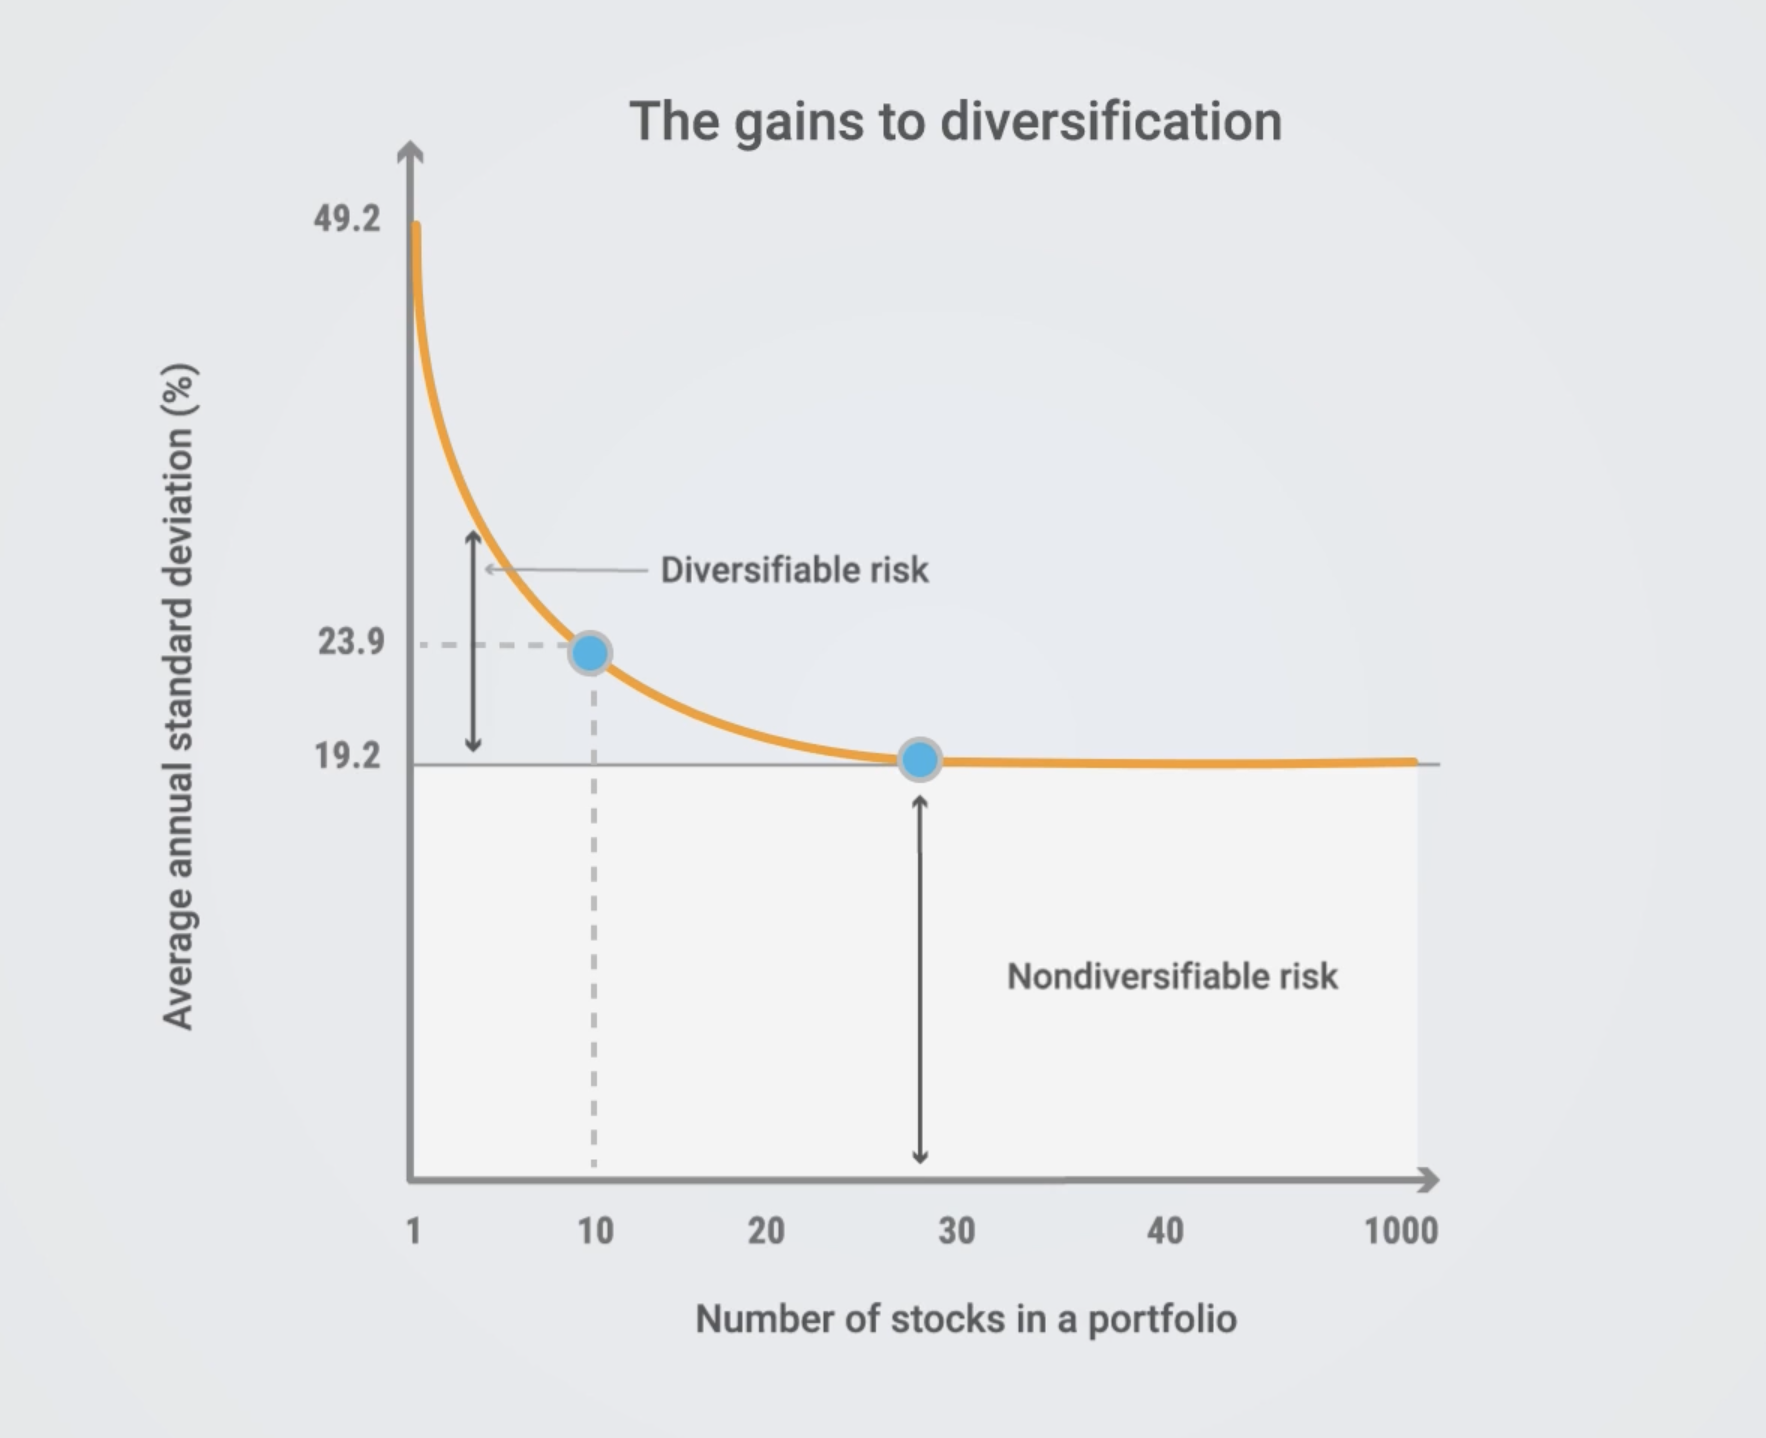
\includegraphics[width=0.5\textwidth]{img/6.2.4.png}
    \caption{Graph showing the diversifiable risk as the number of assets in a portfolio increases}
    \label{fig:diversified_risk}    
\end{figure}

\section{Measuring $\beta$}
\begin{itemize}
    \item A stock's beta, or $\beta$ is a measure of its sensitivity to market movements. 
    \item It is a measure of the stock's systematic risk, or the risk that cannot be diversified away. 
    \item A stock with beta $\beta=1$ in line with the market (identical changes in percentage).
    \item A stock with beta $\beta>1$ moves more than the market. (If the market goes up by 1\%, the stock goes up by more than 1\%)
    \item A stock with beta $0<\beta<1$ moves less than the market. (If the market goes up by 1\%, the stock goes up by less than 1\%)
    \item A stock with beta $\beta=0$ is uncorrelated with the market.
    \item A stock with beta $-1<\beta<0$ moves less than the market, but in the opposite direction. (If the market goes up by 1\%, the stock goes down by less than 1\%)
    \item A stock with beta $\beta=-1$ moves in the opposite direction of the market. (If the market goes up by 1\%, the stock goes down by 1\%)
    \item A stock with beta $\beta<-1$ moves more than the market, but in the opposite direction. (If the market goes up by 1\%, the stock goes down by more than 1\%)

\end{itemize}

\subsection*{The CAPM model}
The Capital Asset Pricing Model (CAPM) states that the expected return of a security is proportionate to its beta multiplied by the market risk premium. Beta is a measure of the security's systematic risk, and the market risk premium is the expected return of the market minus the risk-free rate. This is represented by the formula:

\begin{equation}
    E(R_i) = r_f + \beta_i(E(R_m) - r_f)
\end{equation}

Where:
\begin{itemize}
    \item $E(R_i)$ is the expected return of the security
    \item $r_f$ is the risk-free rate
    \item $\beta_i$ is the beta of the security
    \item $E(R_m)$ is the expected return of the market
    \item $E(R_m) - r_f$ is the market risk premium
\end{itemize}

It can be rewritten as:

\begin{equation}
    \frac{E(R_i) - r_f}{\beta_i} = \frac{E(R_m) - r_f}{\beta_m}
\end{equation}

This is the excess return of any security divided by its beta is consistent among all securities, where $\beta_m$ is the beta of the market which is equal to 1. So the reward for taking on risk is the same for all securities.\\

This forms the basis of an efficient market, where all securities are priced correctly according to their risk. If a security is priced too high or too low, investors will buy or sell the security until the price is correct.\\

\section{CAPM Graphically}
\begin{figure}[H]
    \centering
    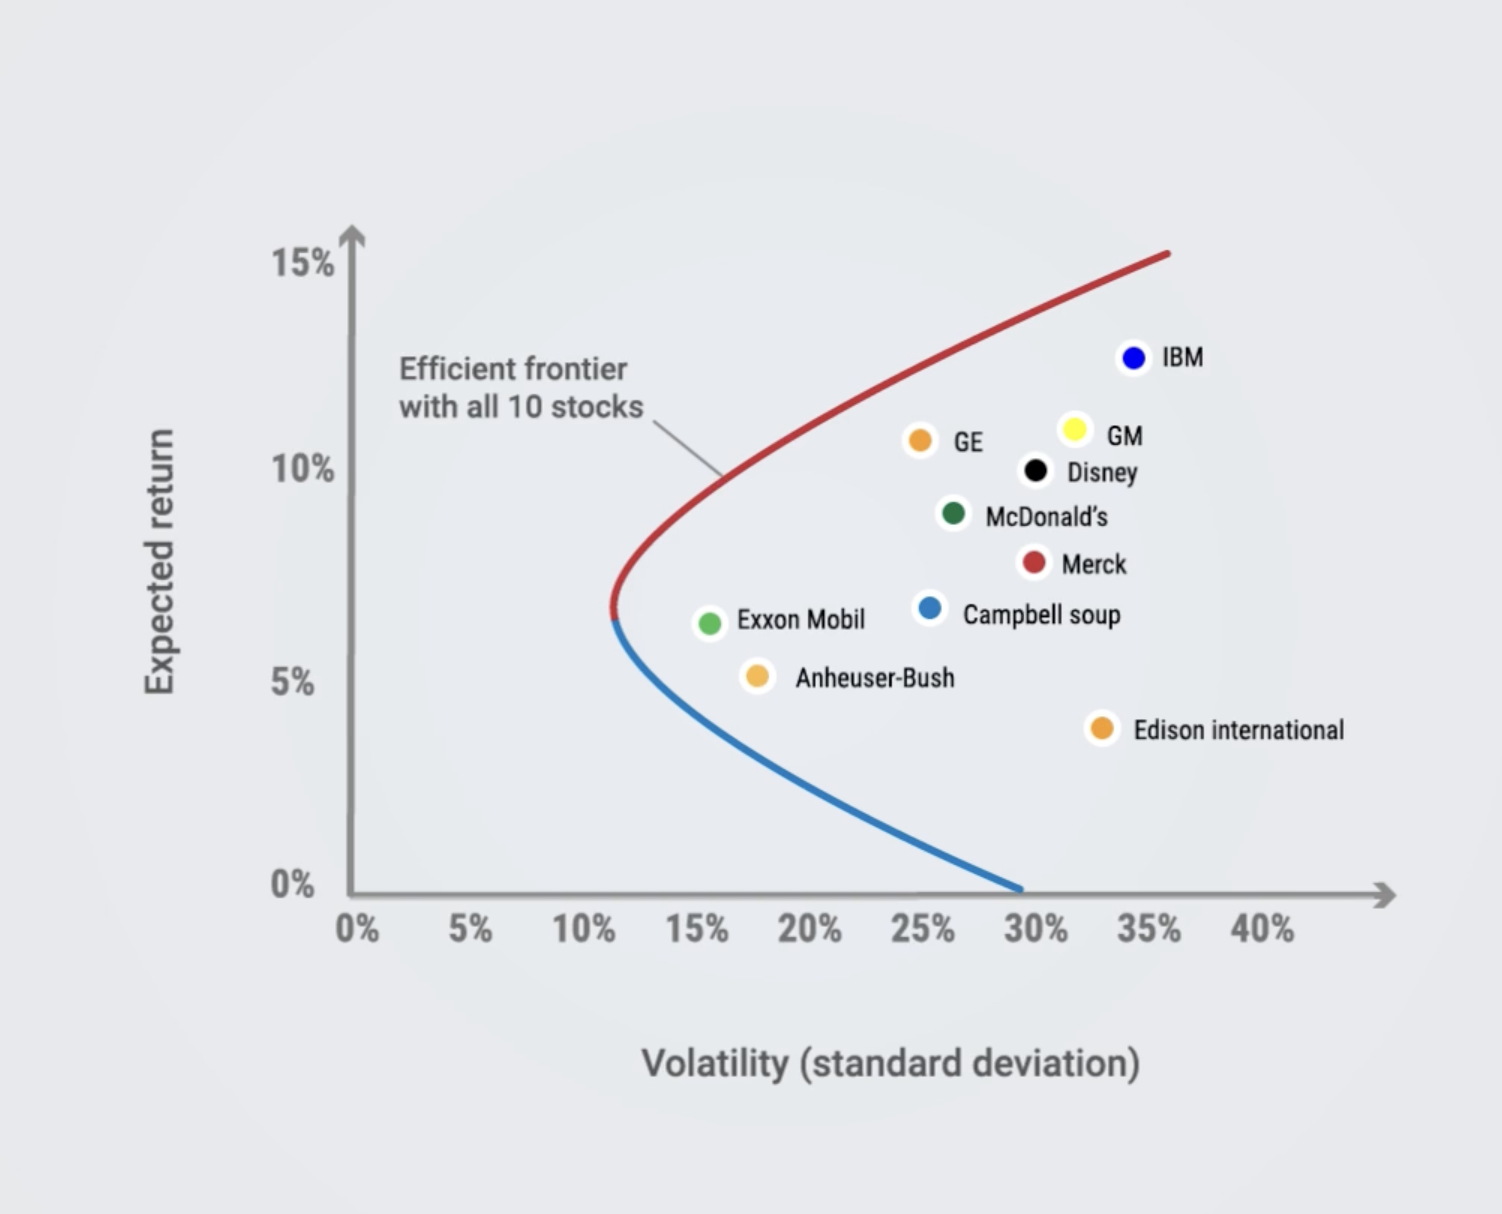
\includegraphics[width=0.6\textwidth]{img/6.5.png}
    \caption{Expected return over volatility, the efficient frontier.}
    \label{fig:capm_graph}
\end{figure}

Investors would only choose portfolios along the efficient frontier, as they offer the highest return for a given level of risk. 

We have a lot more combinations to create portfolios on light blue line, but not all are efficient. The CML is the most efficient portfolio of risky assets that an investor can hold, as it offers the highest return for a given level of risk.\\

\begin{itemize}
    \item Then this introduces the (new) efficient frontier coloured in green, the Capital Market Line (CML), containing the risk-free investment + other risky assets, separate from the efficient frontier that consists of only risky assets, coloured in red.
    \item There is also the market portfolio, that is tangential to combinations of risky assets and the risk-free asset. This market portfolio is the most efficient portfolio that contains only risk assets and no risk-free assets.
    \item The CML represents portfolios as a combination of the market portfolio (investment in risky assets only) and the risk-free asset.
    \item The expected return of a portfolio on the CML is given by the risk-free rate plus a risk premium proportional to the weight in the market portfolio. The volatility of these portfolios are proportional to the weight in the market portfolio (since the risk-free asset has no volatility).
\end{itemize}

\begin{figure}[H]
    \centering
    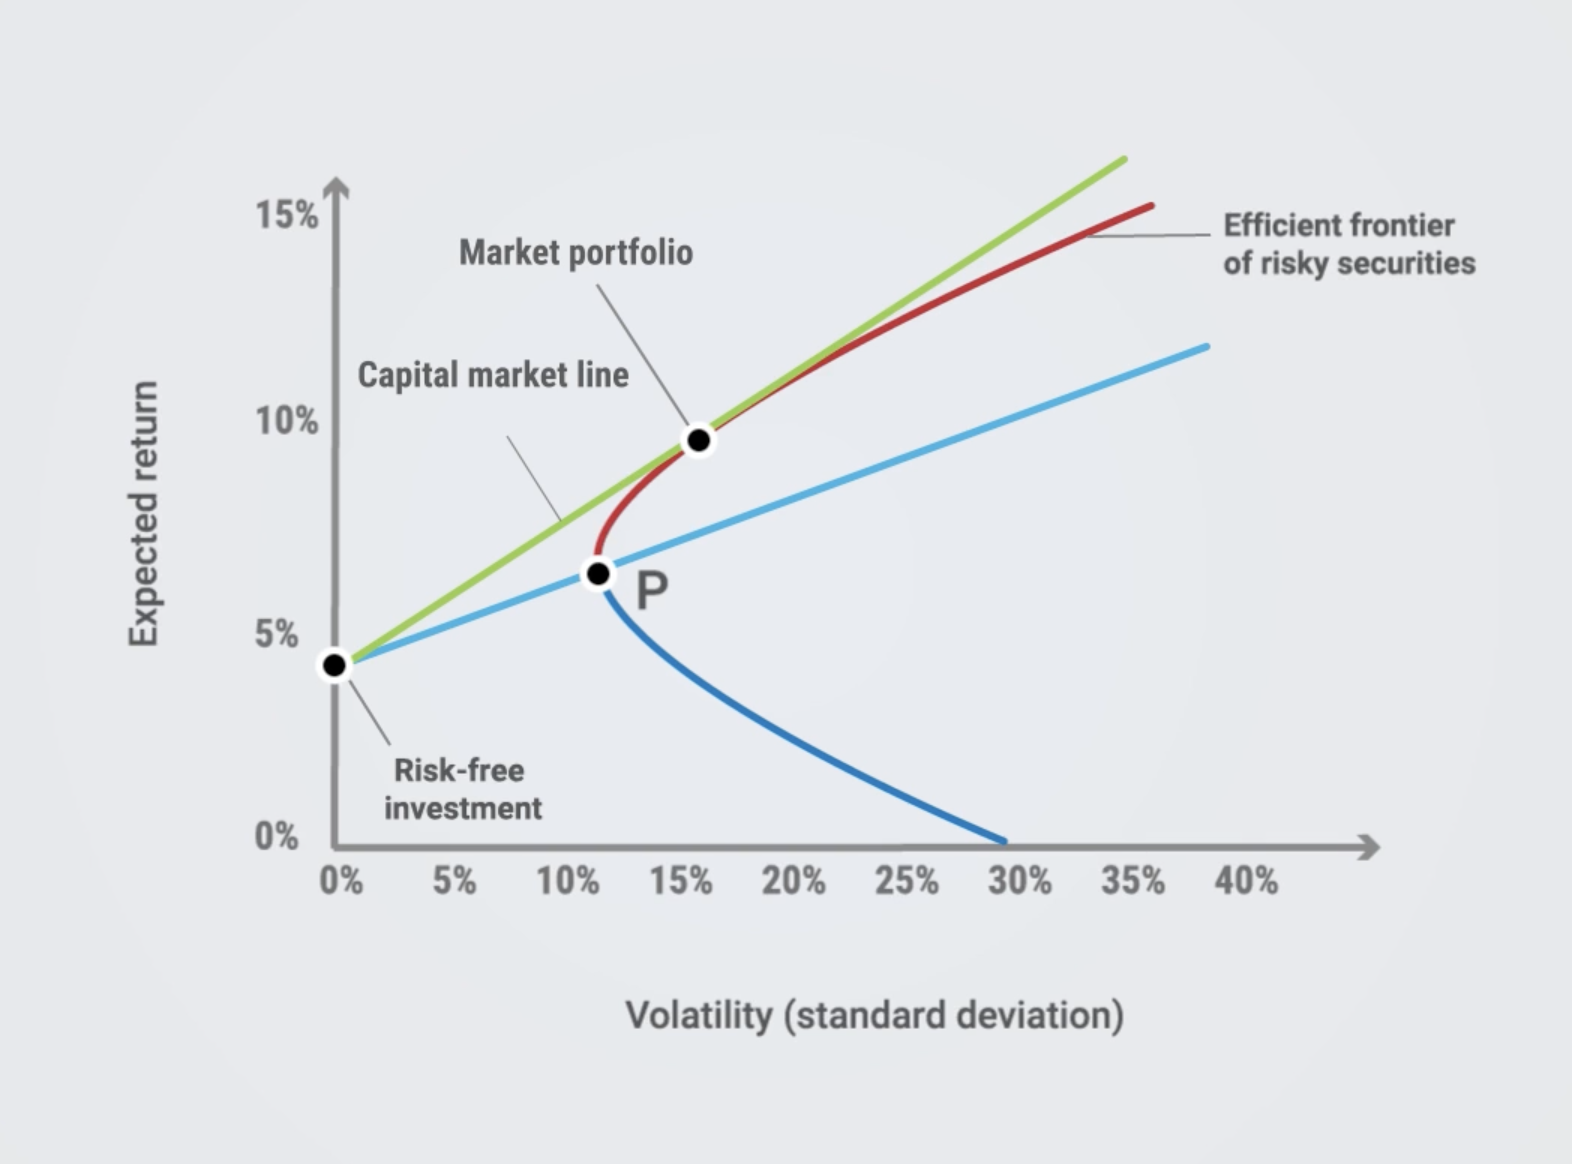
\includegraphics[width=0.6\textwidth]{img/6.6.png}
    \caption{Efficient Frontier and Capital Market Line}
    \label{fig:capm_graph_2}
\end{figure}

As for each individual stock, its level of expected return depends on its level of systematic risk as measured by beta. This relation is expressed graphically by the security market line, or SML.

\begin{figure}[H]
    \centering
    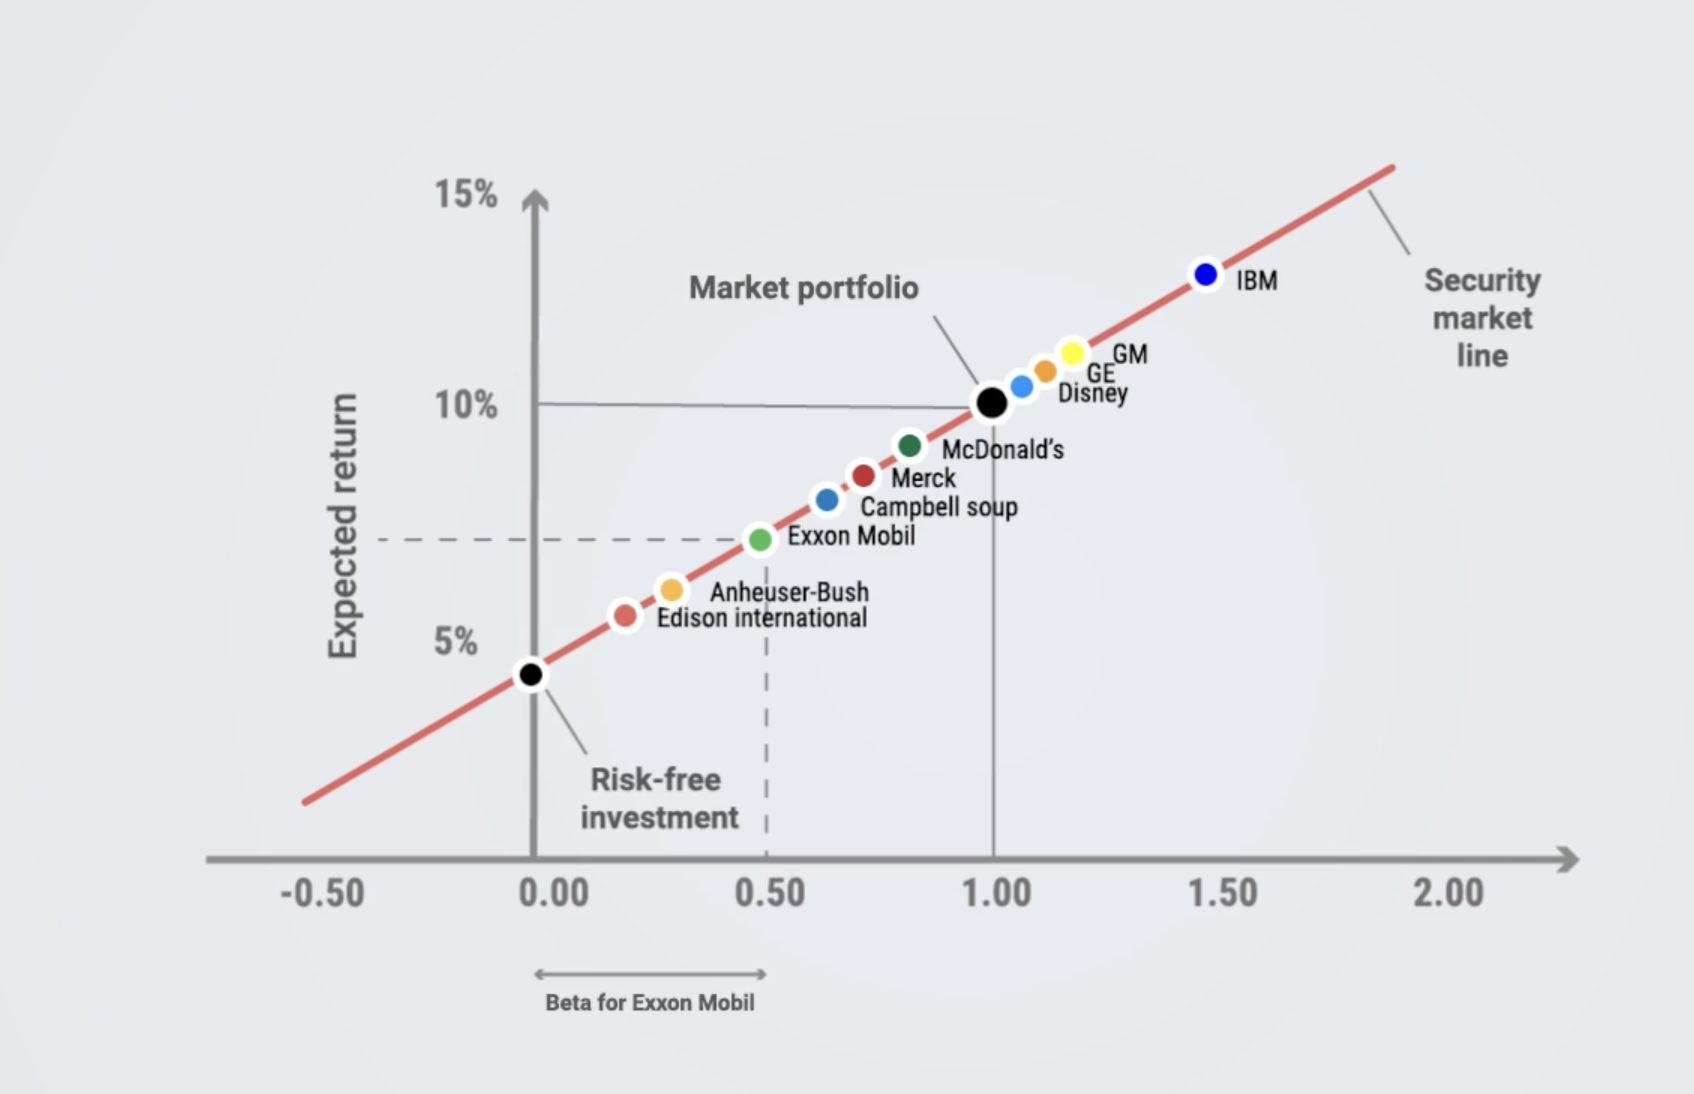
\includegraphics[width=0.6\textwidth]{img/6.7.png}
    \caption{Security Market Line}
    \label{fig:security_market_line}
\end{figure}


\section{Guest Speaker: Mike Kollo Interview}
In this video, Professor James Sefton interviews guest speaker Mike Kollo, who worked at AXA-Rosenberg at the time. They discuss Mike's work as an active portfolio manager.

\noindent \textbf{Key Points Discussed by Mike Kollo:}

\begin{itemize}
    \item \textbf{Market Efficiency and Crisis Impact:} Mike Kollo distinguishes between everyday market scenarios and crisis scenarios, like the 2008 financial crash. In normal conditions, markets integrate information such as earnings reports into prices with relative efficiency, particularly in well-covered, large markets. However, during crises, market dynamics change drastically, leading to rapid price changes and inefficiencies as traditional risk management approaches fail.
    
    \item \textbf{Active Management and Information Flow:} As an active portfolio manager at a quantitative asset management firm, Kollo emphasizes the importance of how information is integrated into market prices. His approach involves systematic analysis to incorporate new data into valuation models, helping predict market movements and enhance investment strategies.
    
    \item \textbf{Technological Advances and Data Integration:} The conversation also touched on the increasing role of technology in asset management. Kollo notes the challenge of filtering and using vast amounts of data effectively, including real-time data from unconventional sources like social media, to inform investment decisions.
    
    \item \textbf{Post-Crisis Industry Changes:} The financial crisis led to a shift in client expectations and industry practices. Investors are increasingly seeking low-volatility investments and outcome-based products. Asset management is moving towards more responsible and client-focused strategies, rather than purely profit-driven approaches.
    
    \item \textbf{Ethical and Educational Role of Asset Management:} Kollo suggests that the future of asset management could involve educating clients about risk and helping them understand the implications of their investments, thus shaping a more ethical and client-oriented industry.
\end{itemize}

\begin{commentbox}{Poll: Would you pay extra for an active portfolio manager?}
32\% answered No, 68\% answered Yes.\\

It is possible to construct a strategy that will outperform the market. For example, according to research mentioned in John H. Cochrane's New Facts in Finance, investing in smaller businesses has been shown to perform slightly better than the market. However, the market efficiency model explains 90-95\% of what is going on; hence, it is popular as a framework for understanding how markets function.\\

In efficient markets, all portfolios (when adjusted for risk) deliver the same return. But how can you adjust for risk? You need a model for this! And only then can you test it for market efficiency. At this point, though, if you do outperform the market, you cannot know for sure if it is because the market is inefficient, or whether your model is wrong. This is difficult to establish and this challenge has been prevalent for a long time!
\end{commentbox}
\chapter{The Cost of Capital}

\section{Introduction}
\begin{itemize}
    \item Overview of the capital structure decision and its significance in determining the cost of capital for a firm.
    \item Exploration of how to estimate the weighted average cost of capital (WACC) of the firm, building upon the previous session's insights on required rates of return by investors based on systematic risk.
    \item Discussion on the capital asset pricing model (CAPM) and the use of the security market line for pricing the required rate of return of an asset.
    \item Application of these concepts to estimate the firm's cost of capital by assessing the costs associated with equity and debt financing.
    \item Introduction to the calculation of the weighted average cost of capital, combining the costs of equity and debt.
    \item Explanation of how to use the WACC to discount future cash flows in financial analysis and investment decision-making.
\end{itemize}

\section{Reading}
Chapters 10 and 12 of Berk, J.B. \& DeMarzo, P.M (2020). Corporate Finance, 5th Edition. Pearson.

\section{The Cost of Capital}

Consider the pros and cons of debt over equity. This chapter focuses more on the tax differences.

\begin{itemize}
    \item Debt is a business expense so it is tax-deductible. This means that the cost of debt is lower than the cost of equity.
    \item Debt can impose discipline on managers to fulfil interest obligations and avoid bankruptcy.
    \item Debt also has lower cost and quicker access to capital. But accumulating too much of it could make it difficult to raise additional funds.
    \item Excessive debt can influence management behaviour to favour riskier projects over safer ones, even if the latter has a higher net present value.
\end{itemize}

Suppose we have two companies A and B with identical operations, profits before interest in taxes (EBIT) of £1M. Company A has no debt but Company B has taken on a loan with interest expense of £200K. Assume the corporate tax rate is 30\%. We thus have the following financial comparison:

\begin{table}[H]
    \centering
    \caption{Financial Comparison of Company A and Company B}
    \begin{tabular}{@{}lcc@{}}
    \toprule
     & \textbf{Company A (No debt)} & \textbf{Company B (With debt)} \\ 
    \midrule
    EBIT & £1,000,000 & £1,000,000 \\
    Interest expense & 0 & £200,000 \\
    Taxable income & £300,000 & £800,000 \\
    Tax (30\%) & £300,000 & £240,000 \\
    Net income & £700,000 & £560,000 \\
    \bottomrule
    \end{tabular}
\end{table}

At first glance, Company A has a significantly higher net income than Company B, but this is where the tax shield comes into play.\\

\begin{equation}
    \text{Tax Shield} = \text{Interest Expense} \times \text{Tax Rate}
\end{equation}

So in this case, the tax shield for Company B is £200,000 $\times$ 30\% = £60,000. This is the savings in taxes that Company B gets. Even though Company B has a lower net income, it has more cash to distribute to shareholders and bondholders.\\

\subsection{Analytical View of the Firm for Capital Structure}
\begin{figure}[H]
    \centering
    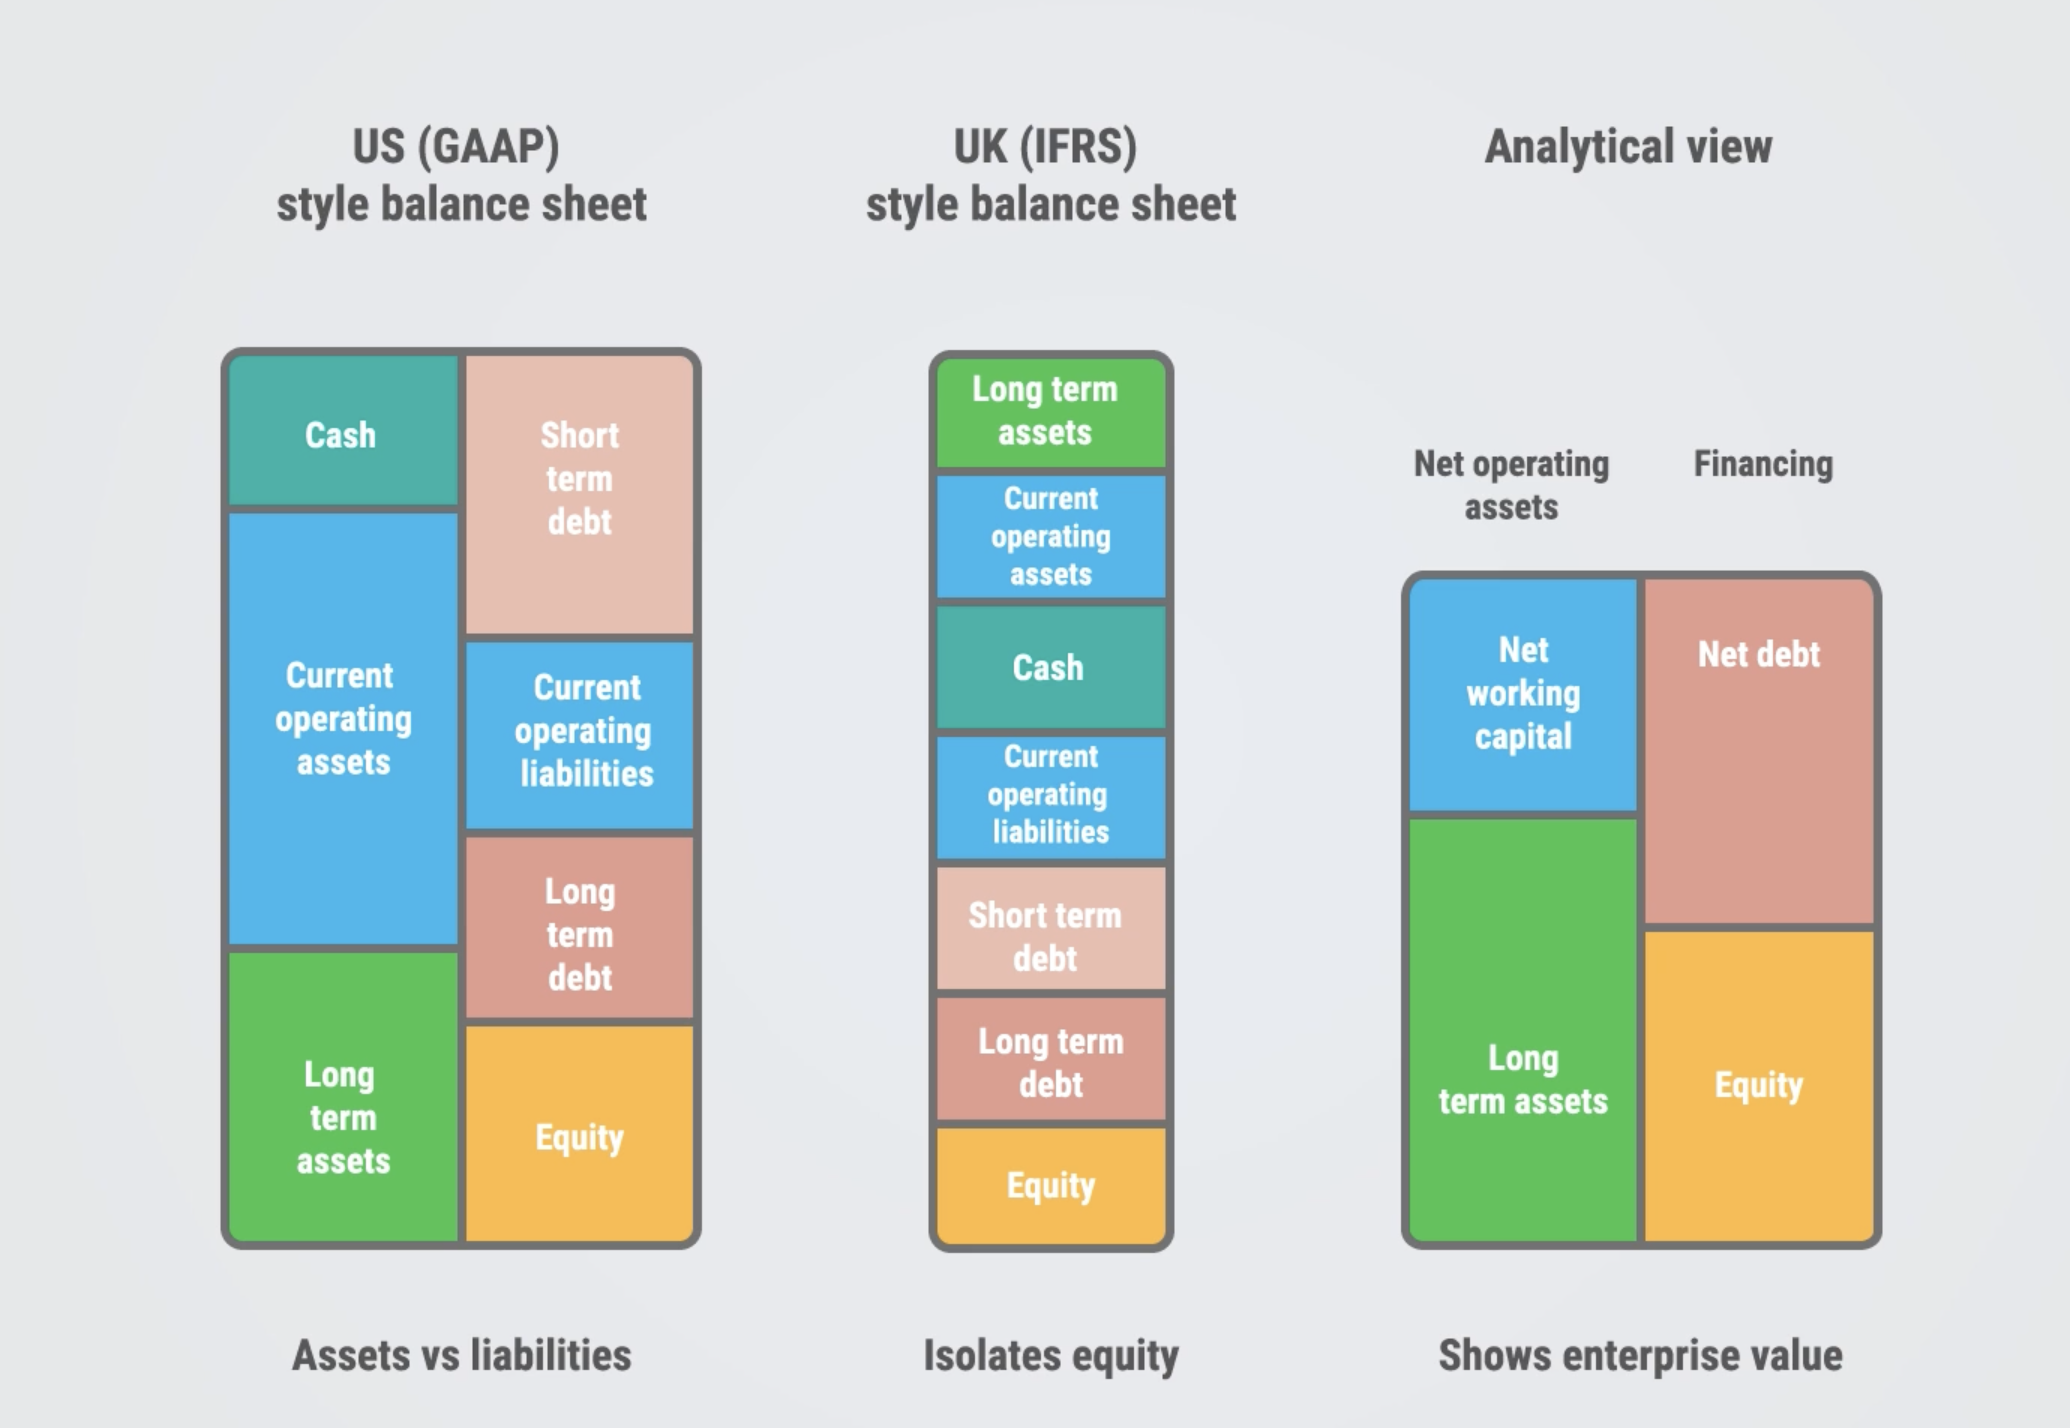
\includegraphics[width=0.8\textwidth]{img/7.3.1.png}
\end{figure}

The balance sheet can be rearranged to show the enterprise value, see Figure \ref{fig:balance_sheet} and Figure \ref{fig:balance_sheet_2}. 

\begin{itemize}
    \item Net working capital
    \item Debt is short-term + long-term debt - cash
    \item Financing of the firm affects cash flows. Debt financing reduces the tax bill, increasing cash flows.
    \item Excessive of debt and the risk of bankruptcy can affect employee and customer behaviour, and suppliers, which could adversely affect cash dlows. 
\end{itemize}

\subsection*{Capital Structure Scenarios}

% \begin{figure}[H]
%     \centering
%     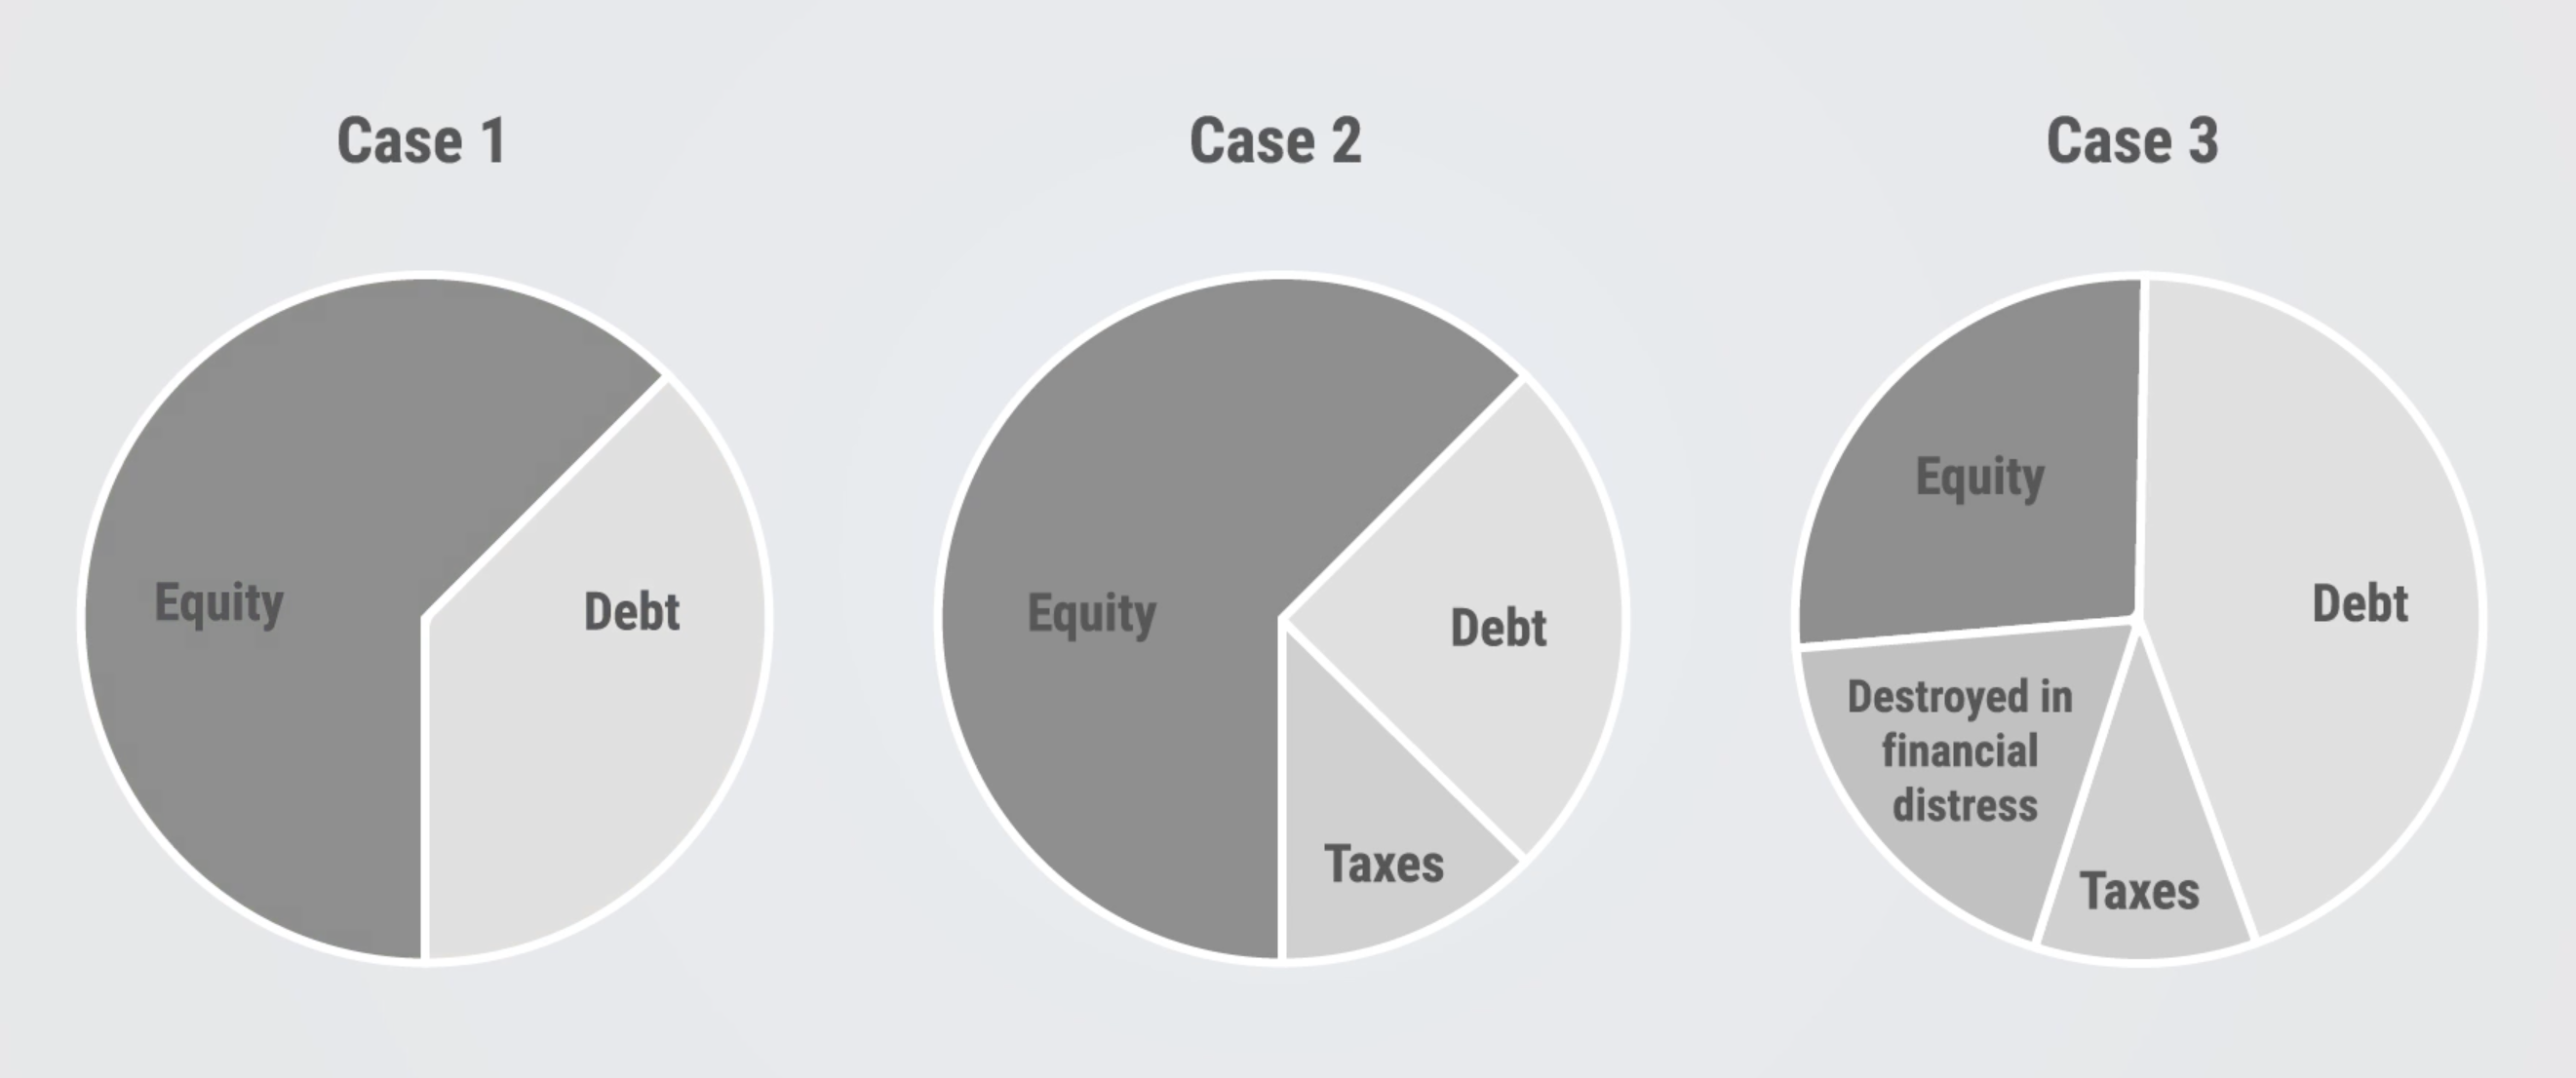
\includegraphics[width=0.8\textwidth]{img/7.3.2.png}
% \end{figure}

\begin{figure}[h]
    \centering
    % Subfigure for Case 1
    \begin{subfigure}{0.3\textwidth}
        \centering
        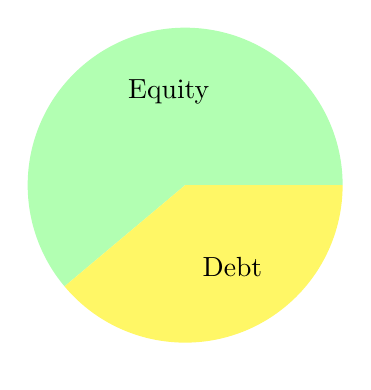
\begin{tikzpicture}
            % Define the slices
            \fill[green!30] (0,0) -- (0:2cm) arc[start angle=0, end angle=220, radius=2cm] -- cycle; % Equity
            \fill[yellow!60] (0,0) -- (220:2cm) arc[start angle=220, end angle=360, radius=2cm] -- cycle; % Debt
            % Labels
            \node at (100:1.2cm) {Equity};
            \node at (300:1.2cm) {Debt};
        \end{tikzpicture}
        \caption{Case 1}
    \end{subfigure}
    % Subfigure for Case 2
    \begin{subfigure}{0.3\textwidth}
        \centering
        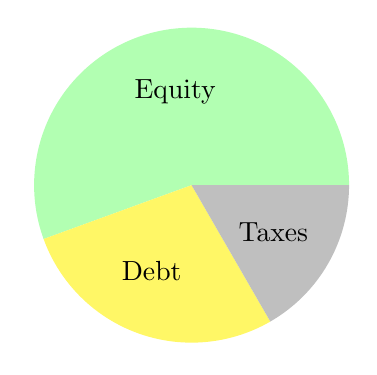
\begin{tikzpicture}
            \fill[green!30] (0,0) -- (0:2cm) arc[start angle=0, end angle=200, radius=2cm] -- cycle; % Equity
            \fill[yellow!60] (0,0) -- (200:2cm) arc[start angle=200, end angle=300, radius=2cm] -- cycle; % Debt
            \fill[gray!50] (0,0) -- (300:2cm) arc[start angle=300, end angle=360, radius=2cm] -- cycle; % Taxes
            % Labels
            \node at (100:1.2cm) {Equity};
            \node at (245:1.2cm) {Debt};
            \node at (330:1.2cm) {Taxes};
        \end{tikzpicture}
        \caption{Case 2}
    \end{subfigure}
    % Subfigure for Case 3
    \begin{subfigure}{0.3\textwidth}
        \centering
        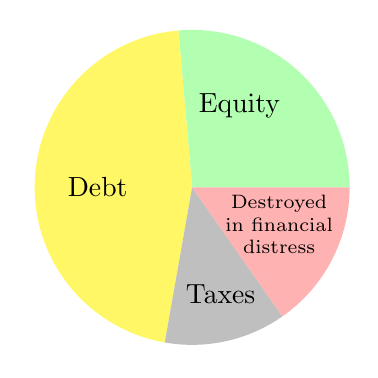
\begin{tikzpicture}
            \fill[green!30] (0,0) -- (0:2cm) arc[start angle=0, end angle=95, radius=2cm] -- cycle; % Equity
            \fill[yellow!60] (0,0) -- (95:2cm) arc[start angle=95, end angle=260, radius=2cm] -- cycle; % Debt
            \fill[gray!50] (0,0) -- (260:2cm) arc[start angle=260, end angle=305, radius=2cm] -- cycle; % Taxes
            \fill[red!30] (0,0) -- (305:2cm) arc[start angle=305, end angle=360, radius=2cm] -- cycle; % Destroyed in financial distress
            % Labels
            \node at (60:1.2cm) {Equity};
            \node at (180:1.2cm) {Debt};
            \node at (285:1.4cm) {Taxes};
            \node[font=\scriptsize, align=center] at (337:1.2cm) {Destroyed \\ in financial \\ distress};

        \end{tikzpicture}
        \caption{Case 3}
    \end{subfigure}
    \caption{Financial composition in three scenarios.}
\end{figure}

\begin{enumerate}
    \item \textbf{Case 1:}
    \begin{itemize}
        \item Perfect capital markets with no taxes or financial distress.
        \item Cash flows are independent of the firm's financing (not affected by financing)
        \item Size of the pie (cash flows) remains constant, financing decisions only affect the size of the slices (cash flows to debt and equity holders)
    \end{itemize}
    \item \textbf{Case 2:}
    \begin{itemize}
        \item Taxes exist in this scenario
        \item Reduces cash paid to investors as some of it goes to the government
    \end{itemize}
    \item \textbf{Case 3:}
    \begin{itemize}
        \item Financial distress costs are present with taxes
        \item Analyse the impact of financial distress on the firm
        \item Size of the pie can decrease due to factors like customer attrition, loss of key employees, reduced credit from suppliers.
        \item This reduces the portion available to debt and equity holders.
    \end{itemize}
\end{enumerate}


\section{Estimating WACC}
This was previously covered in the last chapter's live class.\\

The Weighted Average Cost of Capital (WACC) is the average cost of a company's capital, taking into account the mix of debt and equity used to finance its operations. It is used to discount future cash flows in DCF models to determine the net present value.\\

\begin{equation}
    WACC = \frac{E}{D+E} \cdot r_e + \frac{D}{D+E} \cdot r_d \cdot (1 - \tau_c)
\end{equation}

Where:
\begin{itemize}
    \item $V = E + D$ is the total market value of the firm's financing
    \item $E$ is the market value of equity. $E/V$ is the weight of equity.
    \item $D$ is the market value of debt. $D/V$ is the weight of debt.
    \item $r_e$ is the cost of equity which is required by equity investors. This is estimated using the CAPM model or the Dividend Discount Model (DDM)
    \item $r_d$ is the cost of debt, which can be calculated using the yield to maturity of the firm's existing debt, or considering the interest rate on new debt.
    \item $\tau_c$ is the corporate tax rate. Interest payments on debt are tax-deductible, so $(1 - \tau_c)$ is the tax shield on debt
\end{itemize}

\section{Exercise on Ryanair – Cost of Equity}
Some formulas and a gist of the exercise:
\begin{itemize}
    \item Cost of Equity: $r_e = r_f + \beta \cdot (r_{mkt} - r_f)$ where $r_f$ is the risk-free rate, $\beta$ is the firm's beta, and $r_{mkt}$ is the market return.
    \item Beta can be calculated using the regression of the firm's stock returns against the market returns. 
    \item In Excel, this can be done using the \texttt{lineest(known\_ys, known\_xs, const, stats)} function. Set \texttt{const} and \texttt{stats} to True, and the \texttt{known\_xs} to the excess stock returns, and \texttt{known\_ys} to the market excess returns. The slope of the regression line is the beta.
\end{itemize}

\section{Estimating Debt}
\begin{itemize}
    \item Start by examining the yield to maturity (YTM).
    \item If debt is actively traded, measuring the YTM is straightforward
    \item If debt lacks liquidity or consists of direct loans with the bank, it is more difficult to ascertain market prices and interest rates. Another proxy is needed for the YTM
    \item One proxy approach is to use the company's credit rating or the average credit rating of the debt. 
    \item Another proxy is to use the YTM of debt with a similar rating.
    \item YTM \textbf{assumes no default}, but defaults can occur in practice. 
    \begin{itemize}
        \item To account for this, let the expected return on the debt be the yield to maturity (promised return) minus the expected loss in the event of a default.
        \item The expected loss is calculated as the probability of default multiplied by the loss given a default (LGD).
        \item The probability of default can be estimated from default rates of bonds with similar ratings.
        \begin{equation}
            r_d = YTM - (\text{Probability of Default} \cdot \text{Loss given Default (LGD)})
        \end{equation}
    \end{itemize}
    \item The CAPM and the security market line can also be used to estimate the cost of debt. As corporate bonds tend to be liquid, we can use the debt better of a portfolio of bonds with the same credit rating.
\end{itemize}

\section{Project Valuation}



\begin{itemize}
    \item \textbf{Identify Comparable Companies:} Seek companies specializing in the same products or services. Finding pure play firms can be difficult but focus on those prominently active in the relevant industry.
      \begin{itemize}
        \item \textbf{Pure Play Approach:} Analyse companies within the same industry, e.g., Thomas Cook for package holidays, estimating their betas and adjusting for financial risks.
        \item \textbf{Subjective Approach:} When no perfect match is available, use manual judgement to assess inherent risks. For projects mirroring market average risk, use a beta of 1. If perceived as low-risk, adjust the WACC downward; if high-risk, adjust upward. This approach allows for nuanced consideration of the project's unique characteristics and inherent risks.
      \end{itemize}
    \item \textbf{Estimate Asset Beta:} Determine the asset beta for each identified company. Asset beta (\(\beta_a\)) is calculated using regression analysis and measures the volatility of returns relative to the market.
    \item \textbf{Deleverage Asset Beta:} Convert the asset beta to unlevered beta (\(\beta_u\)) by removing the financial leverage effect, thereby isolating the business risk.
    \begin{equation}
        \beta_u = \frac{\beta_a}{1 + (1 - \tau) \left(\frac{D}{E}\right)}
    \end{equation}
      where \( \tau \) is the tax rate, \( D \) is debt, and \( E \) is equity.
    \item \textbf{Average Unlevered Beta:} Average the unlevered betas of the comparable firms to mitigate individual company variations and better represent the industry’s risk.
    \item \textbf{Adjust for Project Capital Structure:} Modify the averaged unlevered beta to reflect the specific debt-to-equity ratio of the project, thereby tailoring it to the project’s financial structure.
      \begin{equation}
      \beta_{project} = \beta_u \times \left(1 + (1 - \tau) \left(\frac{D}{E}\right)_{project}\right)
\end{equation}
    \item \textbf{Utilise CAPM for Required Return:} Apply the Capital Asset Pricing Model (CAPM) to compute the project's required return:
    \begin{equation}
        r_{required} = r_f + \beta_{project} \times (r_m - r_f)
    \end{equation}
      where \( R_f \) is the risk-free rate, and \( R_m \) is the market return.
  \end{itemize}

  
\chapter{Capital Structure}
\section{Introduction}
\begin{itemize}
    \item Learn how the firm chooses a mix of debt-to-equity.
    \item Assume a perfect capital markets world, but later add taxes and the risk of financial distress.
    \item This chapter will determine the effects of taxes and financial distress on the optimal capital structure.
    \item This chapter also discusses the trade-off theory and finding the optimal debt-to-equity ratio.
\end{itemize}

\section{The Modigliani and Miller Theorem (Case 1)}

\begin{figure}[H]
    \centering
    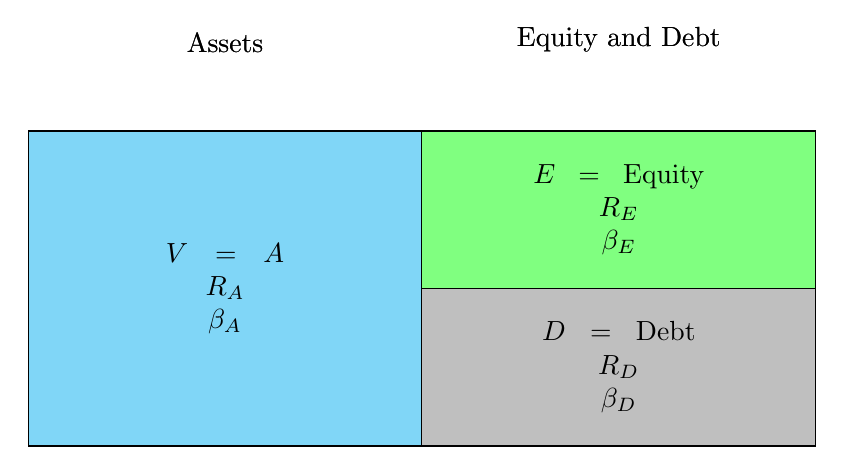
\begin{tikzpicture}
        % Define styles for blocks and labels
        \tikzstyle{assetblock} = [rectangle, draw, fill=cyan!50, text width=5cm, text centered, minimum height=4cm, inner sep=0pt, outer sep=0pt]
        \tikzstyle{equityblock} = [rectangle, draw, fill=green!50, text width=5cm, text centered, minimum height=2cm, inner sep=0pt, outer sep=0pt]
        \tikzstyle{debtblock} = [rectangle, draw, fill=gray!50, text width=5cm, text centered, minimum height=2cm, inner sep=0pt, outer sep=0pt]
        \tikzstyle{labelstyle} = [rectangle, text centered, inner sep=0pt, outer sep=0pt]
        
        % Draw the Asset block
        \node[assetblock] (assets) at (0,0) {$V = A$ \\ $R_A$ \\ $\beta_A$};
        \node[labelstyle, above=of assets] (assetslabel) {Assets};
        
        % Draw the Equity and Debt blocks
        \node[equityblock] (equity) at (5,1) {$E = \text{Equity}$\\$R_E$\\ $\beta_E$};
        \node[debtblock, below=0 of equity] (debt) {$D = \text{Debt}$\\$R_D$\\ $\beta_D$};
        \node[labelstyle, above=of equity] (equitydebtlabel) {Equity and Debt};
        
        % Label column setup
        \node[labelstyle] at (assetslabel) {Assets};
        \node[labelstyle] at (equitydebtlabel) {Equity and Debt};
    \end{tikzpicture}
    \caption{Diagram illustrating the structure of assets, equity, and debt.}
    \label{fig:assets_equity_debt}
\end{figure}

\begin{itemize}
    \item The left-hand side has net operating assets and the right-hand side represents sources of financing. 
    \item In this simple model, as there are no taxes or risk of financial distress, cash flows generated by the firm from its net operating assets are independent of the sources of funding (capital structure). 
    \item \textbf{The firm's value is not affected by the financing method}. 
    \item The free cash flows are easily distributed to the debt and equity holders.
\end{itemize}

\begin{definitionbox}{WACC in Case 1 (No Tax and No Risk of Financial Distress)}
    \begin{equation}
        R_A = WACC = \frac{E}{D+E} \cdot R_E + \frac{D}{D+E} \cdot R_D
    \end{equation}
\end{definitionbox}

$R_A$ is the unlevered assets return as there are no taxes.

\begin{itemize}
    \item As debt is cheaper than debt, it's easy to assume to increasing leverage and taking on more debt will lower the cost of capital and increase the value of the firm.
    \item But how does this reconcile with the fact that cash flows are independent of financing?
    \item This is described by the Modigliani and Miller Theorem, which says as we acquire more debt capital, the equity becomes riskier, leading to a higher rate of return demanded by equity holders, and the cost of equity increases.
    \item So this offsets the benefit of cheaper debt, and the cost of capital remains the same.
\end{itemize}

\begin{theorembox}{Modigliani and Miller Theorem}
    \begin{enumerate}
        \item \textbf{Proposition one: } the firm's value is unaffected by the capital structure, as cash flows are independent of financing sources.
        \item \textbf{Proposition two: } the cost of capital is not influenced by the capital structure.
        
    \end{enumerate}
    \begin{align}
        R_A &= WACC= \frac{E}{D+E} \cdot R_E + \frac{D}{D+E} \cdot R_D\\
        \Rightarrow \underbrace{R_E}_{\text{Cost of Equity Capital}} &= \underbrace{R_A}_{\text{Unlevered Cost of Capital}} + \underbrace{\frac{D}{E} \cdot (R_A - R_D)}_{\text{Risk premium that is increasing on the debt-to-equity ratio}}
    \end{align}

    This is because we can express the cost of equity as a variable that is increasing in the debt-to-equity ratio.\\

    We can express the $\beta_E$, or the equity beta, in a similar manner.
    \begin{align}
        \beta_A &= \frac{E}{D+E} \cdot \beta_E + \frac{D}{D+E} \cdot \beta_D\\
        \Rightarrow \underbrace{\beta_E}_{\text{Equity Beta}} &= \underbrace{\beta_A}_{\text{Business Risk or Unlevered Beta}} + \underbrace{\frac{D}{E} \cdot (\beta_A - \beta_D)}_{\text{Risk premium that is increasing on the debt-to-equity ratio}}
    \end{align}
\begin{itemize}
    \item Equity beta ($\beta_E$) represents the risk of a firm's equity, accounting for its level of leverage. It is derived from the unlevered beta ($\beta_A$), which is the beta of the firm without debt, and adjusted (adding an extra risk-premium ratio) based on the firm's debt-to-equity ratio. 

    \item As leverage (debt-to-equity ratio) increases, the equity beta ($\beta_E$) also increases, indicating a higher risk associated with the equity of the firm. This is because the risk of default and financial distress increases with more debt, placing a higher risk premium on the equity.
\end{itemize}

\end{theorembox}

\begin{examplebox}{Example}
    Suppose we set up a firm that operates for one period and needs to reaise \$1000. Consider two capital structures:

    \begin{figure}[H]
        \centering
        \begin{tabular}{lccc}
        \toprule
        Economic Condition & Firm Earnings & All Equity Case & 50\% Debt Finance ($R_D = 5\%$) \\
        \midrule
        Good economy (50\%) & 14 (+40\%)   & 14 (+40\%)      & 17.5 (+75\%) \\
        Bad economy (50\%)  & 9 (-10\%)    & 9 (-10\%)       & 7.5 (-25\%) \\
        \bottomrule
        \end{tabular}
        \caption{Comparison of firm earnings in different economic conditions and financing scenarios}
    \end{figure}
    

    \begin{itemize}
        \item 100\% equity financing
        \item 50-50 debt-equity financing
    \end{itemize}

    Firm's performance depends on the state of the economy, let's assume it can be either strong or weak with the same probability 50-50.

\begin{itemize}
    \item For the fully-equity financed firm, all the operating income goes to equity holders
    \item The all-equity case will give a return of 14 in a good economy and 9 in a bad economy, translating to a 40\% increase in a good economy and a 10\% decrease in a bad economy.
    \item In the mixed capital structure, some of the income is used to pay off debt holders. This increases the return in a good economy to 17.5, a 75\% increase, and decreases the return in a bad economy to 7.5, a 25\% decrease.
    \item Notice how much more volatile the returns of a 50-50 debt-equity financed firm are compared to the all-equity financed firm. It has almost effectively doubled.
    \item This is why equity holders will demand more returns given the risk.
    \item The WACC for the all-equity firm given both states of the economy is 15\%, netting a positive expected return.
    \item The WACC for the 50-50 debt-equity firm is 25\%, so even though there is a risk of a more negative return, the expected return is higher than the all-equity financed firm.
    \begin{align}
        WACC_{\text{All Equity}} = R_E &= \frac{E}{D+E} \cdot R_E + \frac{D}{D+E} \cdot R_D \\
                                       &= 0.5 \times (40\%) + 0.5 \times (-10\%) = 15\%\\
        WACC_{\text{50-50 Debt-Equity}} = R_E &= \frac{E}{D+E} \cdot R_E + \frac{D}{D+E} \cdot R_D\\
                                        &= 0.5 \times (75\%) + 0.5 \times (-25\%) = 25\%
    \end{align}

\end{itemize}

\end{examplebox}

\begin{figure}[H]
    \centering
    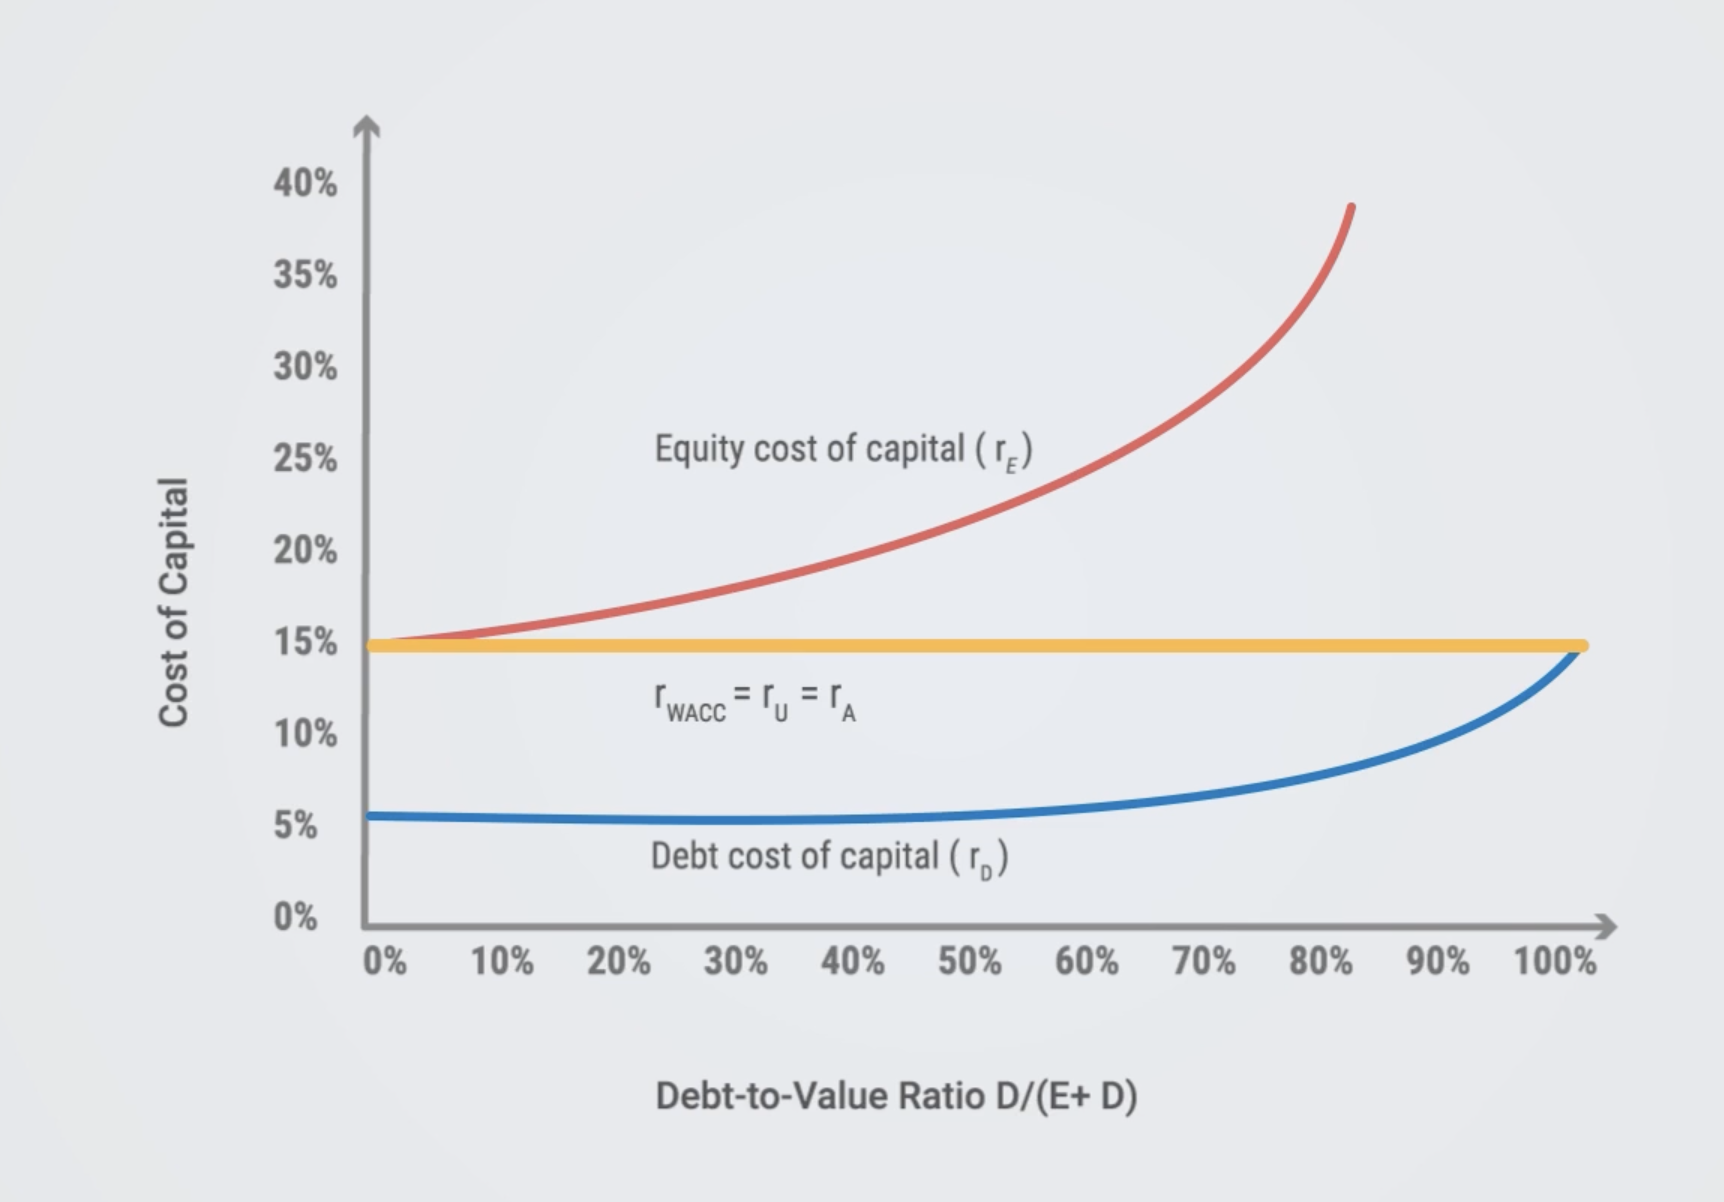
\includegraphics[width=0.7\textwidth]{img/8.2.png}
    \caption{Graph visualisation of the cost of capital over debt-to-value ratio}
\end{figure}

$r_{WACC}$, or the weighted average cost of capital, is constant regardless of the capital structure. This is because the increase in the debt cost of capital offsets the gain from cheaper financing. The red and blue lines sum together to form the yellow line.


\section{Modigliani and Miller's Theorem in a more realistic world (Case 2)}

We now incorporate taxes into our model (case 2), which are tax deductible. This means that the cost of debt is reduced by the tax shield.

\begin{enumerate}
    \item We could use the WACC method that assumes a constant debt-to-equity ratio as the firm grows, and reduce the cost of debt in proportion to the corporate tax rate $\tau_c$.
    \item Another method is the adjusted present value method, more flexible, and does not assume a constant debt-to-equity ratio. It involves calculating the unlevered value of the firm as if it were all equity-financed, and then discounting expected tax savings over time using an appropriate cost of capital.
\end{enumerate}


\subsection*{WACC method for calculating the cost of capital}
\begin{definitionbox}{WACC in Case 2 (With Corporate Tax and No Risk of Financial Distress)}
    For the WACC method, the WACC be expressed as such (note in some equations, $V = D + E$ is used in the denominator):

\begin{align}
    WACC &= \underbrace{\frac{E}{D+E} \cdot R_E}_{\text{Cost of Equity Weighted}} + \underbrace{\frac{D}{D+E} (1-\tau_C) \cdot R_D}_{\text{After-Tax Cost of Debt Weighted}}\\
         &= \underbrace{\frac{E}{D+E} \cdot R_E + \frac{D}{D+E} \cdot R_D}_{\text{Let this be }R_U \text{in the case of D=0}}\ - \ \tau_C \cdot \frac{D}{D+E} \cdot R_D\\
         &= \underbrace{R_U}_{\text{Unlevered Cost of Capital (assuming 100\% equity structure)}} - \underbrace{\tau_C \cdot \frac{D}{D+E} \cdot R_D}_{\text{Reduction due to tax shield}}
\end{align}

\end{definitionbox}

We discount the tax shield by $(1-\tau_C)$, where $\tau_C$ is the corporate tax rate. This is because interest payments are tax-deductible, so the tax shield is the interest payment multiplied by the tax rate.\\

$R_U$ is required return rate on equity for unleveraged firm, taking the case of $D=0$ and thus $R_U = R_E$.\\

This implies cost of equity can be expressed as the unlevered cost of capital plus the difference between the unlevered cost of capital and the cost of debt.

\begin{figure}[H]
    \centering
    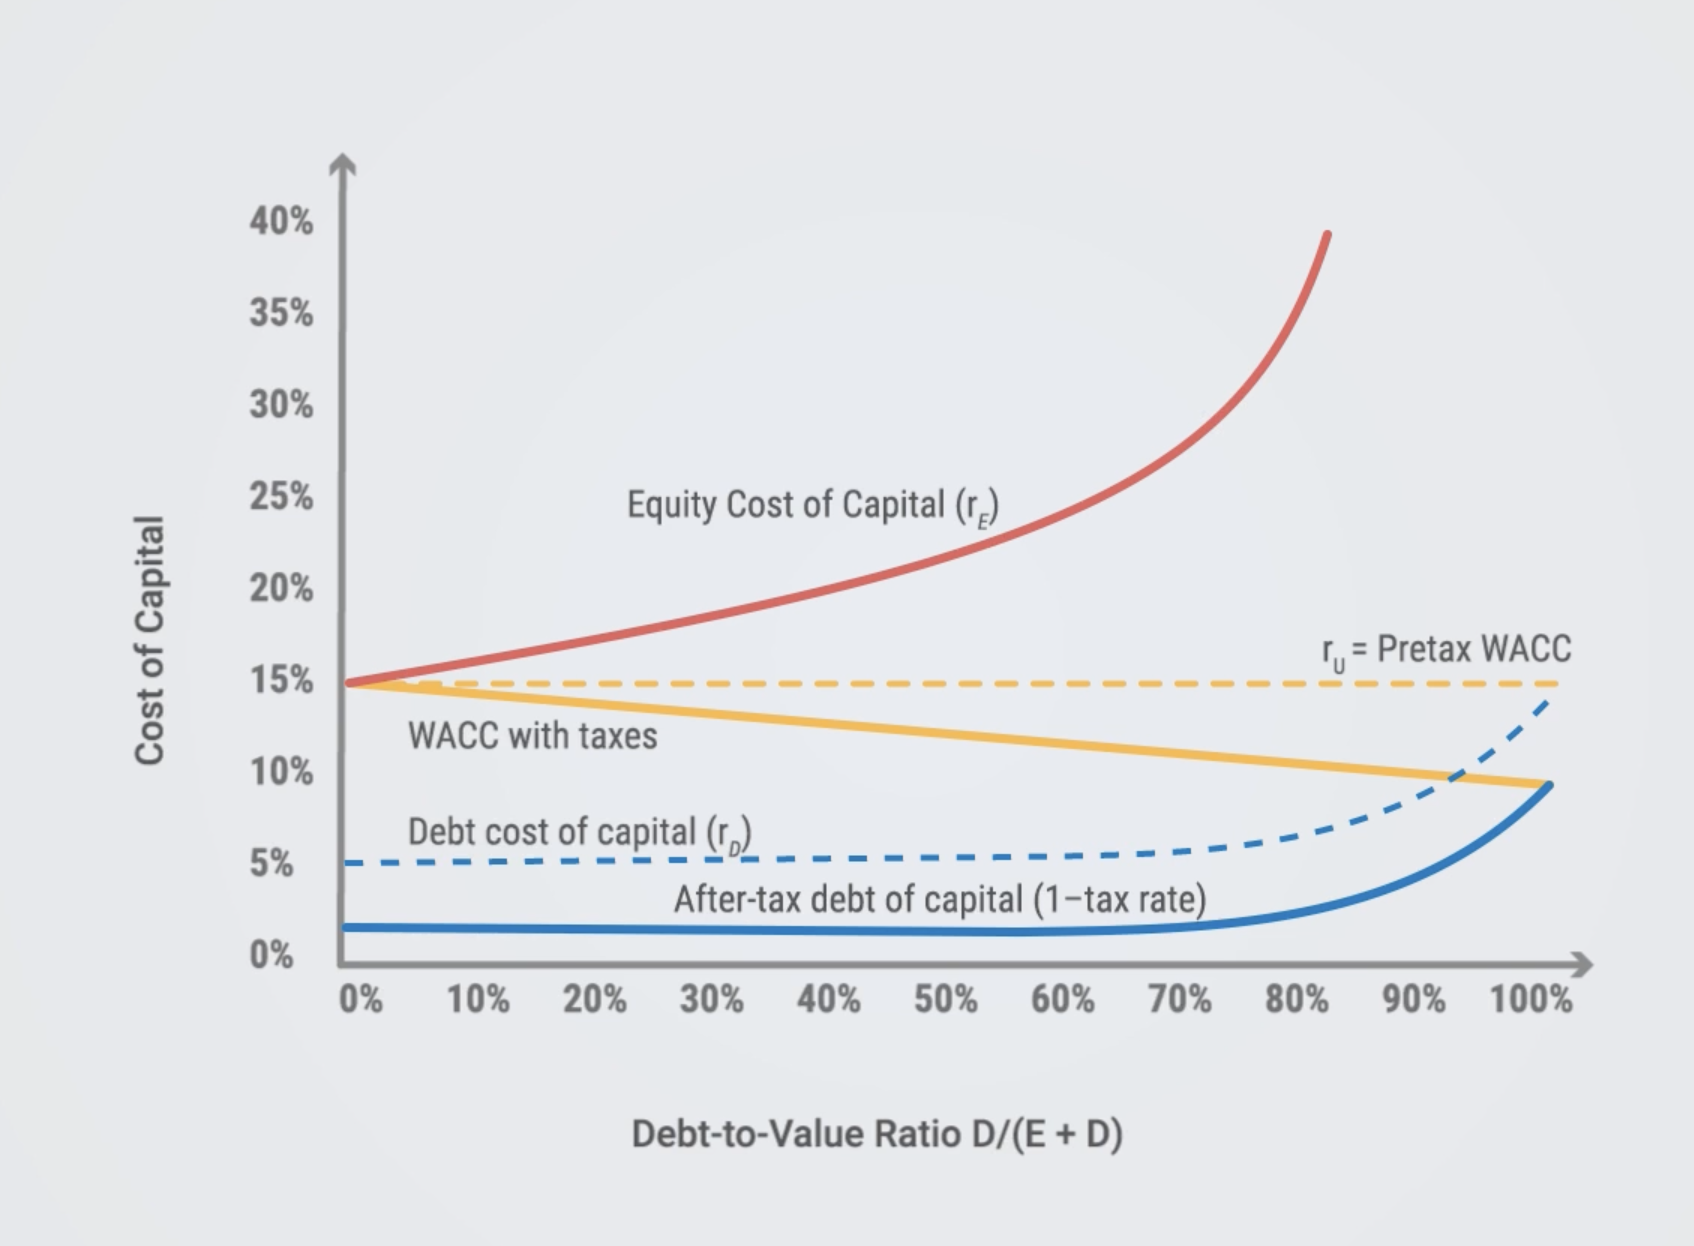
\includegraphics[width=0.7\textwidth]{img/8.3.png}
    \caption{Graph visualisation of the cost of capital over debt-to-value ratio with taxes}
\end{figure}

The issue with this model now is that we are now incentivised to maximise debt without limits, because the corporate tax rate is a fixed discount rate, so we can go all out on debt and reduce the cost of capital indefinitely.

This is where the third case comes in, incoporating the risk of financial distress. 

\begin{examplebox}{True or False?}
\begin{enumerate}
    \item When capital markets are perfect, the portfolio of a firm’s equity and debt replicates the returns we would earn if the firm were unlevered. \textbf{True}
    \item If we can identify a comparison firm whose assets have the same risk as the firm being evaluated, and if the comparison firm is levered, then we can use its equity cost of capital as the cost of capital for our evaluation. \textbf{False}
    
    \item We can calculate the cost of capital of the firm’s assets by computing the weighted average of the firm’s equity and debt cost of capital, which we refer to as the firm’s Weighted Average Cost of Capital (WACC). \textbf{True}
    
    \item When estimating the market value of a firm’s asset, we must use a discount rate that is appropriate given the risk of the firm’s free cash flow. \textbf{True}
\end{enumerate}
\end{examplebox}
\begin{examplebox}{Ungeared vs Geared Firm}
    \textbf{Question 1:} Consider two firms, Geared and Ungeared, that have identical assets that generate identical cash flows. Assume no taxes and no risk of default. Ungeared is an all-equity firm, with 1 million shares outstanding, which trade for a price of \$24 per share. Geared has 2 million shares outstanding and \$12 million dollars in debt at an interest rate of 5\%. If there is no opportunity for capital arbitrage, the stock price for Geared will be:
    
    \textbf{Answer:} \$6.00
    

    \begin{align*}
    \text{Total value of Ungeared} &= 1,000,000 \times \$24 = \$24,000,000 \\
    \text{Total debt of Geared} &= \$12,000,000 \\
    \text{Total equity value of Geared} &= \$24,000,000 - \$12,000,000 = \$12,000,000 \\
    \text{Number of shares of Geared} &= 2,000,000 \\
    \text{Stock price for Geared} &= \frac{\$12,000,000}{2,000,000} = \$6.00
    \end{align*}
    
    \textbf{Question 2:} If Ungeared has a cost of equity capital of 10\%, what is the cost of equity capital of the Geared firm?
    

    
    Let \( R_E \) be the cost of equity capital for the Ungeared firm, and \( R_E' \) be the cost of equity capital for the Geared firm. The cost of equity capital for the Geared firm can be calculated as follows:\\

    Using the Modigliani-Miller theorem:
    \begin{align*}
    R_E' &= R_E + (R_E - R_D) \left(\frac{D}{E}\right) \\
         &= 10\% + (10\% - 5\%) \left(\frac{\$12,000,000}{\$12,000,000}\right) \\
         &= 10\% + 5\% = 15\%
    \end{align*}
    
\end{examplebox}

\begin{examplebox}{Canton Corporation Financial Analysis}
    \textbf{Question:} The unlevered cost of capital for Canton Corporation is 10\%. The firm is financed with 30\% debt that offers a promised return of 15\% and has an expected return of 8\%. Canton is in the 40\% marginal tax bracket.
    
    \textbf{What is Canton's WACC?}
    
    \textit{Answer:}
    \begin{align*}
   \text{WACC} &= R_U - \tau_c \frac{D}{V} R_D \\
               &= 10\% - 0.4 \times 0.3 \times 8\% \\
               &= 10\% - .96\% = 9.04\%
    \end{align*}

    (For WACC, we use only expected return on debt, not the promised return.)
    
    \textbf{What is Canton’s expected cost of equity financing?}
    
    \textit{Answer:} 
    \begin{align*}
        R_E &= R_A + \frac{D}{E} (R_A - R_D) \\
            &= 10\% + \frac{0.3}{0.7} (10\% - 8\%) \\
            &= 10.86\%
    \end{align*}
\end{examplebox}


\begin{examplebox}{Analysis of Change in Capital Structure}
    \textbf{Question:} Your firm has a before-tax return of \$1,800 on an investment of \$800 and a marginal tax rate of 25\%. The unlevered cost of capital is 10\%. The firm currently uses 30\% debt financing with an expected return of 7\%. If it increases its use of debt to 40\%, the expected return on the debt will be 8\%.
    
    \textbf{Calculate your firm's WACC under the current capital structure.}
    
    \textit{Answer:}
    \begin{align*}
    \text{WACC} &= R_U - \tau_c \frac{D}{V} R_D \\
               &= 10\% - 0.25 \times 0.3 \times 7\% \\
               &= 10\% - 0.525\% = 9.48\%
    \end{align*}
    
    \textbf{Calculate your firm's WACC under the proposed capital structure.}
    
    \textit{Answer:}
    \begin{align*}
    \text{WACC} &= R_U - \tau_c \frac{D}{V} R_D \\
               &= 10\% - 0.25 \times 0.4 \times 8\% \\
               &= 10\% - 0.8\% = 9.2\%
    \end{align*}
\end{examplebox}
    







\subsection*{Adjusted Present Value (APV) method}
\begin{sidenotebox}{APV Method}
    The Adjusted Present Value (APV) approach is used to value a firm by considering the effects of debt separately from the operating assets. The APV method can be particularly useful in scenarios where the capital structure is complex or changing. The APV is calculated as follows:

\begin{align}
    APV &= V_U + PV(\text{Tax Shield}) \\
    V_U &= \sum_{t=1}^{T} \frac{FCF_t}{(1 + R_U)^t}
\end{align}

Where:
\begin{itemize}
    \item \( V_U \) is the value of the unlevered firm (i.e., the firm if it had no debt).
    \item \( FCF_t \) is the free cash flow to the firm at time \( t \).
    \item \( R_U \) is the unlevered cost of capital.
    \item \( T \) is the number of periods.
    \item \( PV(\text{Tax Shield}) \) is the present value of the tax shield due to debt.
\end{itemize}


\subsection*{Calculating the Present Value of the Tax Shield}

The tax shield can be calculated using the corporate tax rate \( \tau_C \) and the debt \( D \) as follows:

\begin{align}
    PV(\text{Tax Shield}) &= \tau_C \cdot D \cdot \frac{1 - (1 + R_D)^{-T}}{R_D}
\end{align}

Where:
\begin{itemize}
    \item \( R_D \) is the cost of debt.
    \item \( D \) is the total amount of debt.
    \item \( \tau_C \) is the corporate tax rate.
    \item \( T \) is the number of periods the debt is held.
\end{itemize}

\subsection*{Advantages of APV}

The APV method allows for the flexibility of adjusting the valuation for different financing scenarios. It is especially useful when:
\begin{itemize}
    \item The firm's capital structure is changing over time.
    \item The risk profile of debt is different from that of the firm’s assets.
\end{itemize}

\subsection*{Comparison to WACC}

Unlike the WACC method, which requires an assumption of a constant target capital structure, APV separates the value of the firm into components. This separation can provide more clarity in situations where the financing mix is not stable or predictable.
\end{sidenotebox}

\section{Live Class: Capital Structure in Practice (Case 3)}
In the Live Class, Diageo is analysed as an example to find the right balance between debt and equity.
\subsection*{Diageo Case Study}

\begin{itemize}
    \item Diageo is one of the largest food and drink companies in the world.
    \item Initially, it had three main businesses: 
    \begin{enumerate}
        \item Alcoholic beverages
        \item Packaged Foods
        \item Fast food restaurants
    \end{enumerate}
    \item In the 2000s, there were major changes in the core business:
    \begin{enumerate}
        \item Selling their packaged food subsidiary (Pillsbury) to General Mills for \$5.1 billion in cash plus 141 million shares of General Mills (about 33\% of Market Cap)
        \item Spin-off of Burger King
        \item A lot changed on the left-hand side (Assets) of the Balance Sheet; a good opportunity to optimise the right-hand side (Debt and Equity Financing) as well – historically conservative (See \ref{fig:assets_equity_debt} for balance sheet diagram.)
    \end{enumerate}
\end{itemize}


\subsection*{Optimum Capital Structure}
\begin{theorembox}{Trade-Off Theory}
    The trade-off theory of capital structure suggests that firms have a target capital structure that balances the benefits of debt (such as tax shields and lower cost of capital) with the costs of debt (such as financial distress and agency costs). The optimal capital structure is the one that maximises the firm's value by balancing these trade-offs.
\end{theorembox}


\begin{figure}[H]
    \centering
    \begin{subfigure}{0.55\textwidth}
        \centering
        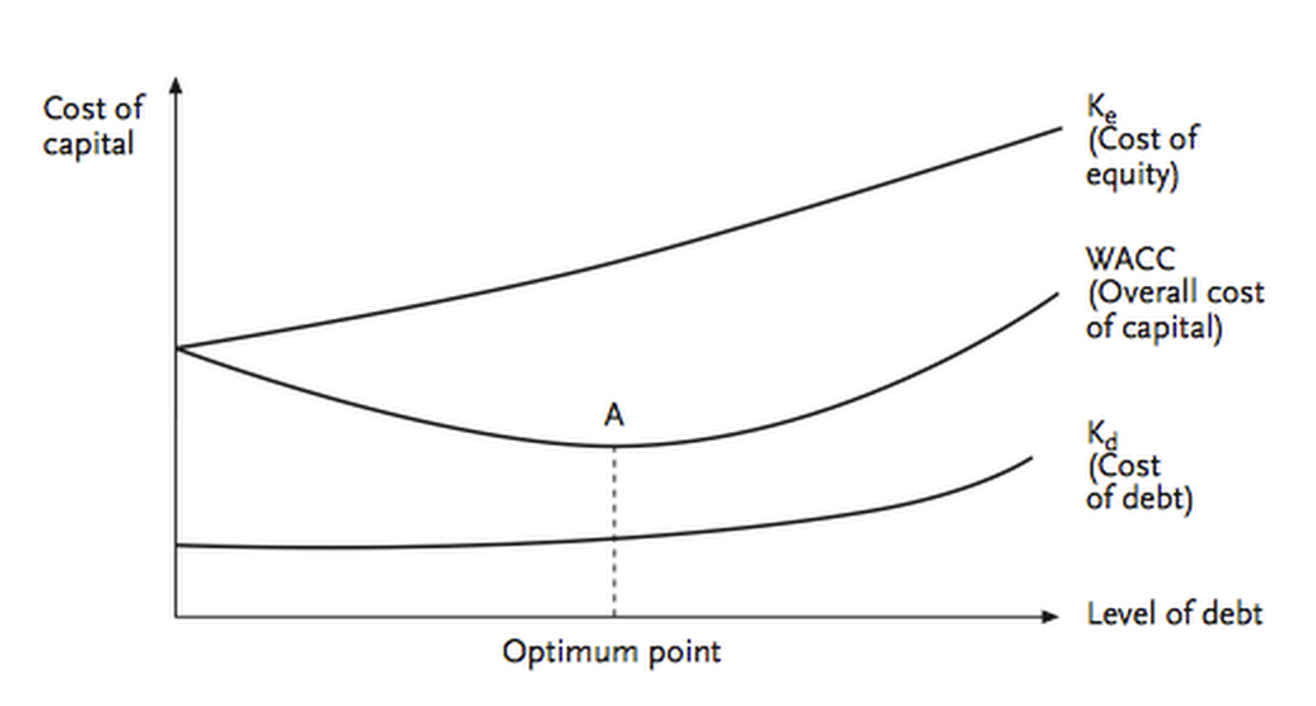
\includegraphics[width=\textwidth]{img/8.4.1.png}
        \caption{The Weighted Average Cost of Capital}
    \end{subfigure}

    \begin{subfigure}{0.55\textwidth}
        % \centering
        % 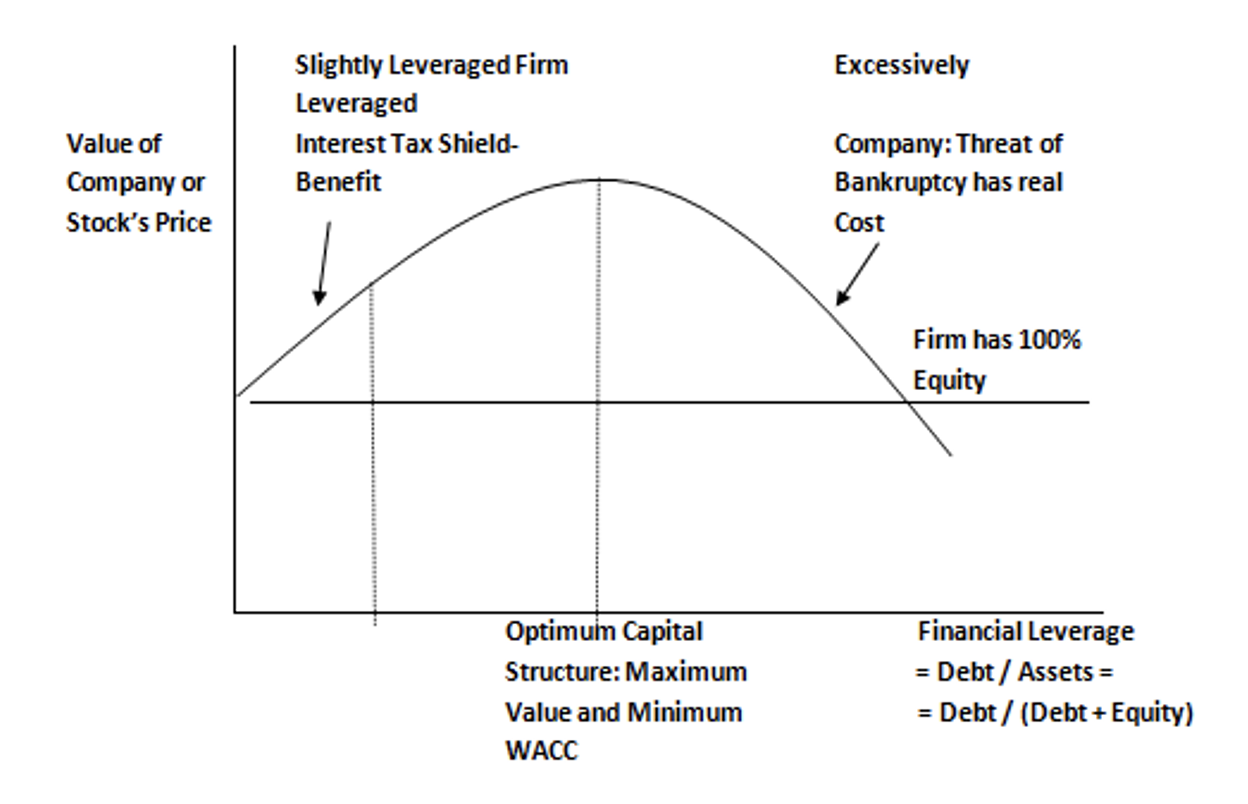
\includegraphics[width=\textwidth]{img/8.4.2.png}
        % \caption{Firm Value and the Optimum Capital Structure}
        \centering
        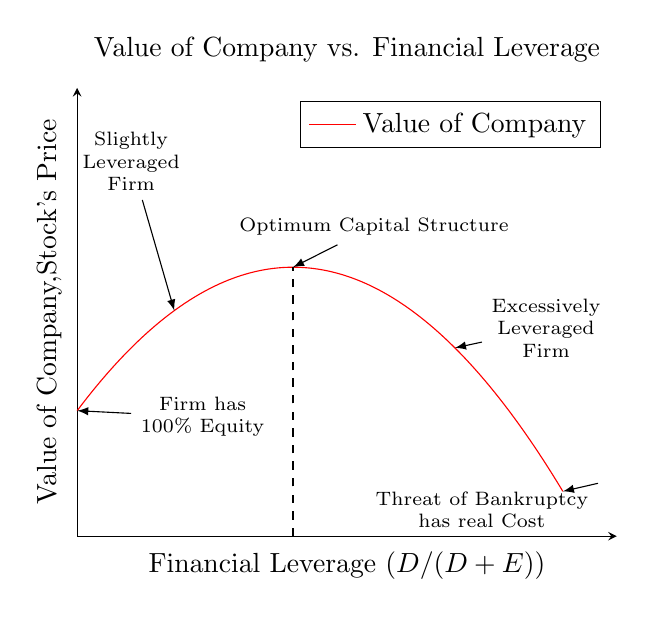
\begin{tikzpicture}
        \begin{axis}[
            title={Value of Company vs. Financial Leverage},
            xlabel={Financial Leverage (\( D / (D+E) \))},
            ylabel={Value of Company,Stock's Price},
            xmin=0, xmax=1,
            ymin=0, ymax=100,
            xtick=\empty, xticklabels={},
            ytick=\empty, yticklabels={},
            legend pos=north east,
            grid style=dashed,
            axis lines = left,
            clip=false,
        ]
        
        % Adding the parabolic curve
        \addplot[
            domain=0:0.9, 
            samples=100, 
            color=red,
        ]
        {-200*(x-0.4)^2 + 60};
        \addlegendentry{Value of Company}
        
    % Nodes with connecting arrows
    \node (sl) at (axis cs:0.1,75) [anchor=south, font=\scriptsize, align=center] {Slightly \\ Leveraged\\ Firm};
    \draw[-latex] (sl) -- (axis cs:0.18,50.32);
    
    \node (ex) at (axis cs:0.75,55) [anchor=north west, font=\scriptsize, align=center] {Excessively \\ Leveraged\\ Firm};
    \draw[-latex] (ex) -- (axis cs:0.7,42);
    
    \node (eq) at (axis cs:0.1,20) [anchor=south west, font=\scriptsize, align=center] {Firm has \\100\% Equity};
    \draw[-latex] (eq) -- (axis cs:0,28);
    
    \node (bn) at (axis cs:0.75,12) [anchor=north, font=\scriptsize, align=center] {Threat of Bankruptcy\\ has real Cost};
    \draw[-latex] (bn) -- (axis cs:0.9,10);

    \node (op) at (axis cs:0.55, 65) [anchor=south, font=\scriptsize, align=center] {Optimum Capital Structure};
    \draw[-latex] (op) -- (axis cs:0.4,60);
    
    % Adding dashed lines for visual aid
    \draw[dashed] (axis cs:0.4,0) -- (axis cs:0.4,60);
    
    
        % Adding dashed lines for visual aid
        \draw[dashed] (axis cs:0.4,0) -- (axis cs:0.4,60);
        
        \end{axis}
        \end{tikzpicture}
        \caption{The relationship between financial leverage and company value, showing the optimum capital structure.}
    \end{subfigure}
    \caption{Graphs showing the optimum point of capital structure}
\end{figure}


\subsection*{Leveraged Recapitalisation}
Leveraged recapitalisation is a strategy used by companies to increase their debt levels and reduce their equity levels. This can be done by issuing debt and using the proceeds to buy back shares or pay a special dividend to shareholders. This increases leverage while maintaining the same share price. 

\begin{figure}[H]
    \centering
    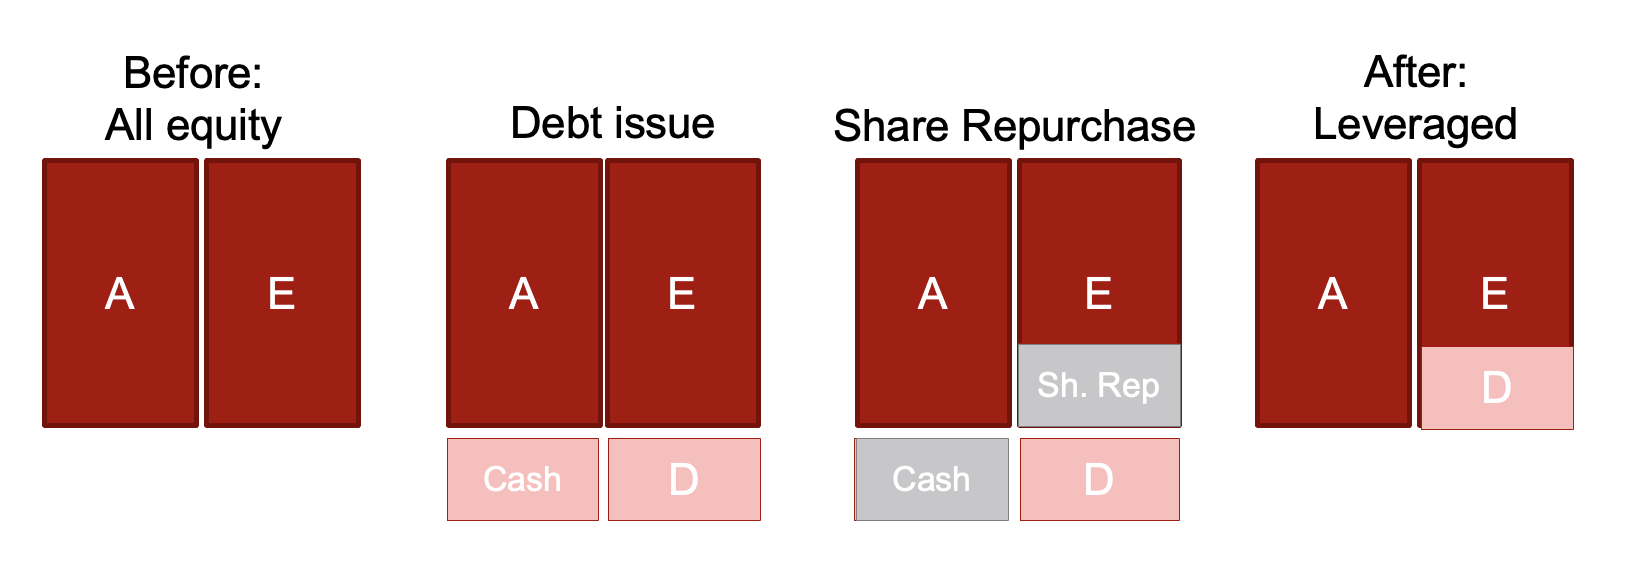
\includegraphics[width=0.7\textwidth]{img/8.4.3.png}
    \caption{Diagram of Leveraged Recap}
\end{figure}

\subsection*{Before the Recap}
\begin{itemize}
    \item Assets: \$3.5M
    \item Financing (100\% Equity): \$3.5M
    \item Discount Rate: 20\%
    \item Tax Rate: 30\%
    \item Interest Rate: 10\%
\end{itemize}


Income Statement:
\[
\begin{array}{lr}
    \text{EBIT} & 1,000,000 \\
    \text{- Taxes} & 300,000 \\
    \hline
    \text{= Net income} & 700,000 \\
\end{array}
\]


Net income is \$700K.
To get \$3.5M:

\begin{align*}
    \$ 3,500,000 = \sum^{\infty}_{t=1}\frac{\$700,000}{1.2^t} = \frac{\$700,000}{.2}
\end{align*}


\subsection*{After the Recap}
\begin{itemize}
    \item Assets: \$3.5M + Tax Shield: (\$0.3M)  
    \item Financing: \$3.8M (\$2.8M Equity, \$1M Debt)
\end{itemize}

Income Statement:
\[
\begin{array}{lr}
    \text{EBIT} & 1,000,000 \\
    \text{- Interest} & 100,000 \\
    \text{Taxable Income} & 900,000 \\
    \text{- Taxes} & 270,000 \\
    \hline
    \text{= Net income} & 630,000 \\
\end{array}
\]

The annual tax shield is $\$300,000-\$270,000 = \$30,000$.

To calculate value of the firm (\$3.8M):
\begin{align*}
 \$ 3,800,000 &= \sum^{\infty}_{t=1} {\frac{\$700,000}{1.2^t}} + \sum^{\infty}_{t=1} {\frac{\$30,000}{1.1^t}}\\
   &= \frac{\$700,000}{0.2} + \frac{\$30,000}{0.1} = \$3,800,000
\end{align*}

We discount using 1.1 for the tax shield, because it is the discount rate minus the interest rate

\subsection*{What Happens to the Share Price?}

\subsubsection*{Before the Recap}
\begin{itemize}
    \item Assets: \$3.5M
    \item Financing (100\% Equity): \$3.5M
\end{itemize}

\subsubsection*{After the Recap}
\begin{itemize}
    \item Assets: \$3.5M + Tax Shield: (\$0.3M)  
    \item Financing: \$3.8M (\$2.8M Equity, \$1M Debt)
\end{itemize}

Assume $m=1M$ shares outstanding before recap.

\begin{itemize}
    \item $P_0 = \$3.5$ (Before Recap)
    \item Share buyback. Let's say we have $D=\$1M$ to buy back at $p=\$3.5$ per share. 
    \item We will buy $n$ shares. So $n = 1M/3.5 = 285,714$ shares.
    \item After the buyback:
    \begin{itemize}
        \item Equity Value = \$630,000
        \item \# of shares outstanding = 714,286
        \item New share price = \$2.8M/0.714M = \$3.92
    \end{itemize}
\end{itemize}

We have to choose a $p$ such that shareholders are willing to tender their shares.

\begin{itemize}
    \item $np = D$ where $D$ is the debt we raise to buy back shares.
    \item $np = \$1M$
    \item $(m-n)p = E$ where $E$ is the equity value after the buyback.
    \begin{align*}
        mp - np &= E \\
        \$p \times 1M - \$1M &= \$2.8M \\
        p &= \$3.8
    \end{align*}
    \item $n = \$1M/\$3.8 = 263,158$
\end{itemize}

\subsection*{Taking on Too Much Debt, Costs of Financial Distress}
\begin{itemize}
    \item If the firm loses money, it cannot get the tax deduction
    \item This will negatively affect operations, causing economic distress
    \item Leads to agency problems
    \item Direct impact on bankruptcy costs (bankruptcy costs are a function of the amount of debt)
\end{itemize}

\begin{table}[h]
    \centering
    \caption{S\&P Credit Ratings with Average EBIT/Interest and Debt/Capital Ratios. A rating of BBB and higher is considered investment grade, while ratings below BBB are considered speculative.}
    \label{tab:credit_ratings}
    \begin{tabular}{lll}
    \toprule
    \textbf{Rating} & \textbf{Avg. EBIT/Interest} & \textbf{Average Debt/Capital (\%)} \\
    \midrule
    AAA & 12.9 & 21.4 \\
    AA  & 9.2  & 29.3 \\
    A   & 7.2  & 33.3 \\
    BBB & 4.1  & 40.8 \\
    \midrule
    \addlinespace 
    BB  & 2.5  & 55.3 \\
    B   & 1.2  & 68.8 \\
    CCC & -0.9 & 71.5 \\
    \bottomrule
    \end{tabular}
\end{table}

\subsection*{Should Diageo Increase Leverage?}

\subsubsection*{Diageo Case Study Recap}

\begin{itemize}
    \item Diageo is one of the largest food and drink companies in the world.
    \item Initially, it had three main businesses: 
    \begin{enumerate}
        \item Alcoholic beverages
        \item Packaged Foods
        \item Fast food restaurants
    \end{enumerate}
    \item In the 2000s, there were major changes in the core business:
    \begin{enumerate}
        \item Selling their packaged food subsidiary (Pillsbury) to General Mills for \$5.1 billion in cash plus 141 million shares of General Mills (about 33\% of Market Cap)
        \item Spin-off of Burger King
        \item A lot changed on the left-hand side (Assets) of the Balance Sheet; a good opportunity to optimise the right-hand side (Debt and Equity Financing) as well – historically conservative (See \ref{fig:assets_equity_debt} for balance sheet diagram.)
    \end{enumerate}
\end{itemize}

\subsubsection*{Debt}
\begin{itemize}
    \item \textbf{Tax Shield: }
    \begin{itemize}
        \item Low/high tax rate? 27\%
        \item Tax Loss Carry Forwards: This is a tax provision that allows companies to carry forward losses to future years to offset profits and reduce tax liability.
        \item UK new cap to tax shield: a worldwide group can deduct against its taxable profits to a maximum of 30\% of taxable EBITDA. In other words, the tax shield is limited to 30\% of EBITDA.
        \item Do any other tax credits exist? For example, R\&D. But Diageo does not have them
    \end{itemize}
    \item \textbf{Discipline/Governance: }
    \begin{itemize}
        \item Does Diageo have governance issues?
        \item How is its free cash flow?
    \end{itemize}
    \item \textbf{Risk: }
    \begin{itemize}
        \item Debt cyclicality: Low/high? Current beta on debt is 0.55
        \item Volatility: How is the stability of its cash flows?
        \item Any technological risk? A technological risk could be a new competitor entering the market with a new technology that disrupts the industry. In Diageo's case, none.
        \item Competition risk? Yes, Diageo has many competitors.
        \item Currency risk? Yes, Diageo has currency risk as it is a global company.
        \item Legal risk? Possibly, as it operates in multiple countries, has many brands (risk of IP disputes), and sells alcohol, is large (risk of antitrust and competition law)
        \item Regulation risk? Yes, Diageo is in the alcohol industry, which can be subject to alcohol regulations, marketing restrictions, taxation and duty increases, health and safety regulations, ethics etc.
    \end{itemize}
    \item \textbf{Distress Costs:}
    \begin{itemize}
        \item Investment Needs: Diageo is large, can benefit from economies of scale, possible to grow via organic growth, and M\&A. Can invest in new products/markets/talents/R\&D.
        \item Assets: Mostly low tech tangibles. Intangibles include brand value. 
        \item Competition: High competition, aggressive market players. 
        \item Customers: Will customers stop buying if Diageo is in distress? Does it have a durable competitive advantage?
        \item Employees: The business is human-capital intensive, in R\&D, marketing, process.
        \item Management: Is management capable of managing a highly leveraged firm?
    \end{itemize}
\end{itemize}

\subsection*{Diageo's Checklist}
\subsubsection*{Pros}
\begin{itemize}
    \item Tax-shield?
    \item Governance/Discipline?
\end{itemize}
\subsubsection*{Cons}
\begin{itemize}
    \item Are cash flows risky? Hard to hedge?
    \item What if they got into financial distress?
    \item Financial flexibility?
    \item Liquidity of assets, hard to value/sell/redeploy in the event of a crisis?
    \item Rivals more aggresive?
    \item Customers/Suppliers care?
    \item Employees care?
    \item Management capable?
\end{itemize}

\subsection*{60\% D/A Recap: Value Impact}

Before the recapitalization is announced:
\begin{itemize}
    \item Market equity \( E_{\text{pre-recap}} = £20.144M \)
    \item Debt \( D_{\text{pre-recap}} = £6,882M \)
    \item Firm value \( V_{\text{pre-recap}} = £27,026M \)
\end{itemize}

After the recapitalization is implemented:
\begin{itemize}
    \item Tax shield created \( \text{PVTS} \approx t \times \text{New } D = 30\% \times 418 = £125M \)
    \item Firm value \( V_{\text{post-recap}} = £27,026M + 125M = £27,151M \)
    \item Debt \( D_{\text{post-recap}} = £6,882M + 418M = £7,300M \)
    \item Market equity \( E_{\text{post-recap}} = £27,151M - 7,300M = £19,851M \)
\end{itemize}

Market equity drops but shareholders are better off as overall they get:
\[
E_{\text{at announcement}} = \text{Payout} + E_{\text{post-recap}} = 418M + 19,851M = £20,269M
\]

\subsection*{60\% D/A Recap: Transaction}

\begin{itemize}
    \item Pre-recap, there are 3,397M shares.
    \item Stock price reaction to the recap announcement:
    \begin{itemize}
        \item Stock price pre-recap: £5.93
        \item Stock price at announcement: \( \frac{£20,269M}{3,397M} = £5.97 \)
    \end{itemize}
    \item Diageo repurchases \( \frac{418M}{5.97} = 70M \) shares.
    \item Remaining shares post-recap: \( 3,397M - 70M = 3,327M \) shares.
    \item Stock price post recap: \( \frac{£19,851M}{3,327M} = £5.97 \)
\end{itemize}

\subsection*{Analysis of Recap Values}
\begin{figure}[H]
    \centering
    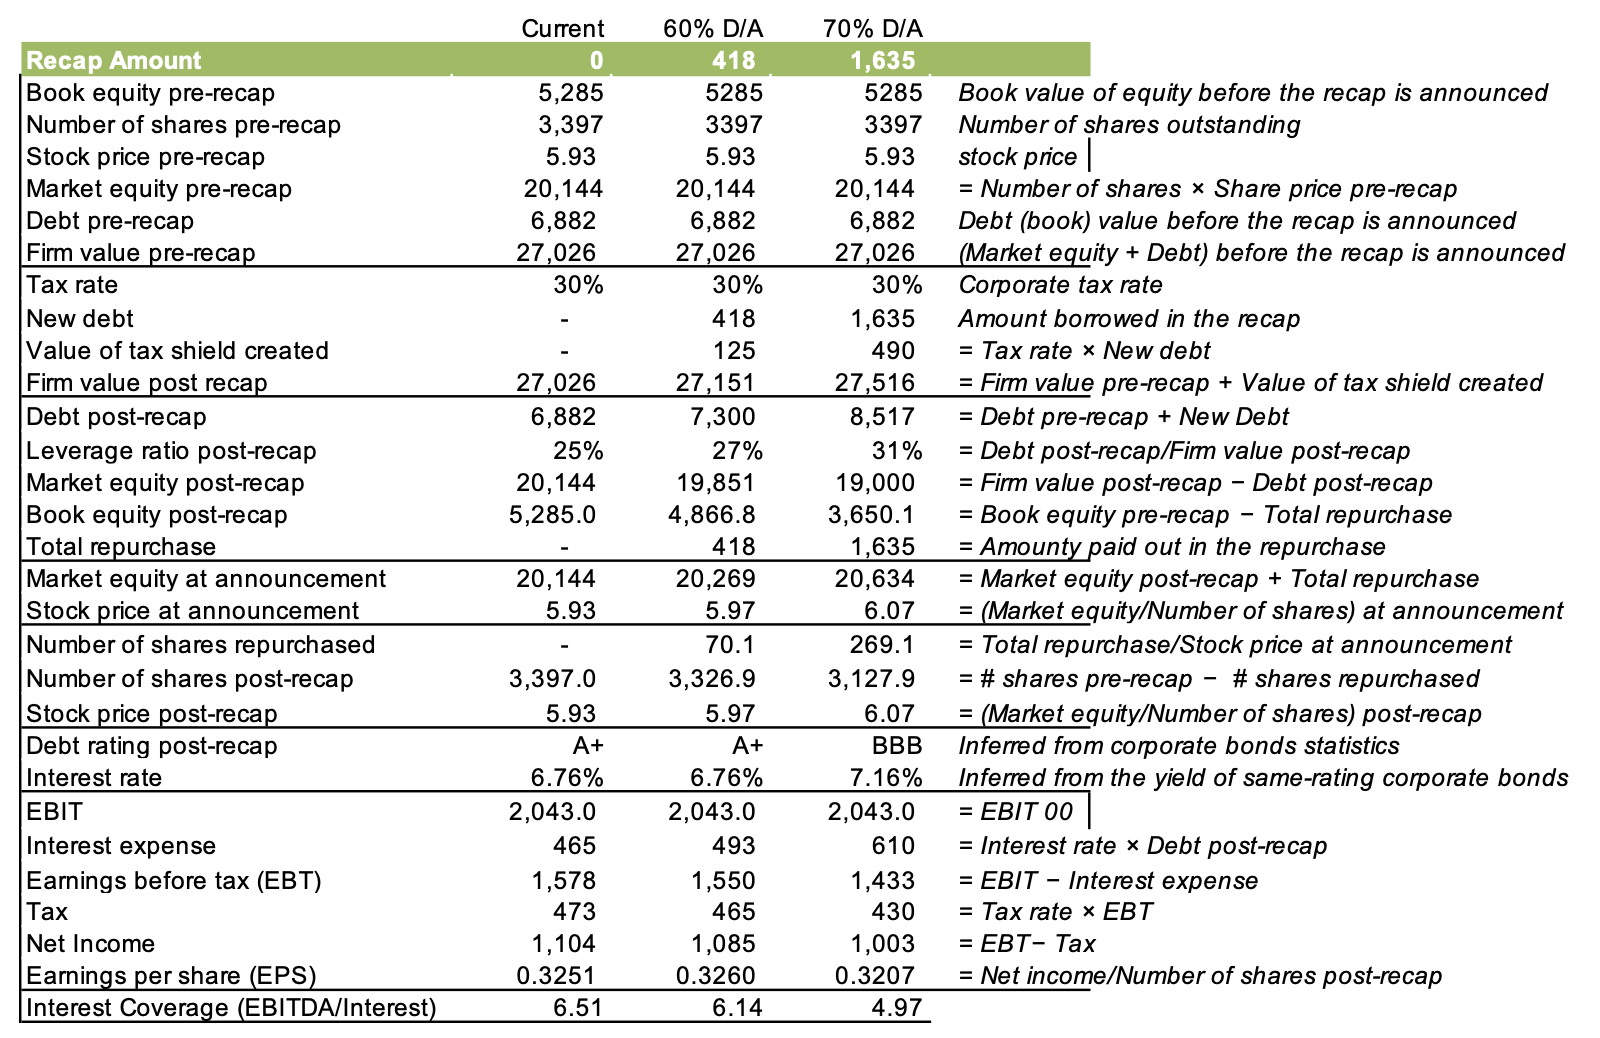
\includegraphics[width=0.95\textwidth]{img/8.4.4.png}
    \caption{Comparison of recap amounts. A higher 70\% D/A amount causes a higher share price, but reduces debt rating and earnings per share.}
\end{figure}

\section{The Private Equity Debate: Podcast}
\subsection*{FOR Private Equity}

\begin{enumerate}
    \item Private equity firms outperform on an operating basis, demonstrating their ability to create value for their investors.
    \item The outperformance of private equity firms, even after accounting for fees, suggests that they are doing something substantial.
    \item Private equity investments provide diversification benefits, as shown by studies comparing them to public stock portfolios.
    \item Dividend recapitalisations, enabled by low interest rates, offer a legitimate way to return value to investors and discipline management.
\end{enumerate}

\subsection*{AGAINST Private Equity}

\begin{enumerate}
    \item Private equity returns may not be as impressive when accounting for the risk involved, particularly due to high leverage.
    \item Private equity firms often mark their own inventory, potentially inflating their performance figures and masking risks.
    \item The practice of selling companies to other private equity firms, rather than strategic buyers, raises questions about the actual value creation.
    \item Some studies indicate that private equity ownership may lead to negative outcomes for society, such as increased mortality rates in certain industries.
    \item Dividend recapitalisations may artificially boost returns without necessarily indicating genuine value creation or company improvement.
\end{enumerate}


\chapter{Options}
\section{Introduction}

\begin{itemize}
    \item Discuss why firms have a risk management policy
    \item Explain the mechanics of the options market and pricing
    \item Produce a payoff at maturity chart
    \item Describe the put-call parity relationship.
\end{itemize}

\section{Options}

\begin{itemize}
    \item Options are prevalent in financial markets and trading strategies.
    \item Three key terms: 'in the money', 'at the money', and 'out of the money' categorize options based on the relationship between the underlying asset's price and the strike price.
\end{itemize}

\subsection*{European Call and Put Options}

\begin{itemize}
    \item European call option: Gives the holder the right to buy the underlying asset at a pre-specified price (strike price) on a predetermined future date (expiry date).
    \item European put option: Grants the owner the right to sell the underlying asset at the strike price on the expiry date.
    \item European options can only be exercised at the expiry date, unlike American options which offer flexibility for early exercise.
    \item The price paid for an option is called the option's premium.
\end{itemize}

\subsection*{Option Categories}

\begin{itemize}
    \item \textbf{In the Money (ITM)}: When the option's intrinsic value is positive because the asset's price is significantly higher (for calls) or lower (for puts) than the strike price. 
    \item \textbf{Out of the Money (OTM)}: When the option's intrinsic value is zero because the asset's price is well below (for calls) or above (for puts) the strike price.
    \item \textbf{At the Money (ATM)}: When the asset's price is close to the strike price. In this region, the speculative value of the option is the primary driver of its price.
\end{itemize}

\subsection*{Value Components of Options}

\begin{itemize}
    \item \textbf{Intrinsic Value}: Only present in ITM options. Represents the difference between the option's exercise price and the spot (current) price of the underlying asset. \textbf{In other words, it is the value of the option if it were to be exercised immediately.}
    \item \textbf{Speculative Value}: The difference between the option's premium and its intrinsic value. ATM and OTM values have zero intrinsic value, so it's equal to the option premium in the case of ATM or OTM. It is influenced by volatility, it is the primary component of at-the-money options (since options become more volatile as they approach the strike price).
\end{itemize}


\begin{examplebox}{Options Questions}
    \textbf{Question 1:} Suppose you have purchased a call option with a strike price of \$50.00 and a premium of \$3.00, and that the current stock price is \$54.00 at expiration. Calculate the payoff of the long call option.

\textbf{Answer:} The payoff of the long call option is $\text{Max}(S - K, 0) - P = \text{Max}(54 - 50, 0) - 3 = 1$\\

\textbf{Question 2:} Suppose you have written (shorted) a call option with a strike price of \$60.00, received a premium of \$5.00, and that the stock price at expiration is \$58.00. Calculate the payoff of the short call option.

\textbf{Answer:} The payoff of the short call option is $-[\text{Max}(S - K, 0) - P] = -[\text{Max}(58 - 60, 0) - 5] = 5$\\

\textbf{Question 3:} Assume you have purchased a put option with a strike price of \$85.00 and a premium of \$6.00, and that the stock price at expiration is \$90.00. Calculate the payoff of the long put option.

\textbf{Answer:} The payoff of the long put option is $\text{Max}(K - S, 0) - P = \text{Max}(85 - 90, 0) - 6 = -6$\\

\textbf{Question 4:} You have sold (shorted) a put option with a strike price of \$75.00, received a premium of \$4.00, and the stock price at expiration is \$70.00. Calculate the payoff of the short put option.

\textbf{Answer:} The payoff of the short put option is $-[\text{Max}(K - S, 0) - P] = -[\text{Max}(75 - 70, 0) - 4] = -1$\\
\end{examplebox}

\section{Options Payoff Structures}

Options trading involves the agreement between two parties to facilitate the potential transaction on an underlying security at a predetermined price, known as the strike price (\(K\)), before a specified date. The buyer of the option acquires the right, but not the obligation, to execute the transaction.

\subsection*{Long Call}

A long call option gives the holder the right to buy the underlying asset at the strike price (\(K\)). The payoff for a long call option is given by:
\[ \text{Payoff} = \max(0, S_T - K)-\text{premium} \]
where \( S_T \) is the price of the underlying asset at maturity.\\

\textbf{Example:} Consider a long call option with a premium of 10, with a strike price of \( K = 100 \). If at maturity, the asset price is \( S_T = 120 \), the payoff is \( \max(0, 120 - 100) -10 = 10 \).

\begin{figure}[H]
    \centering
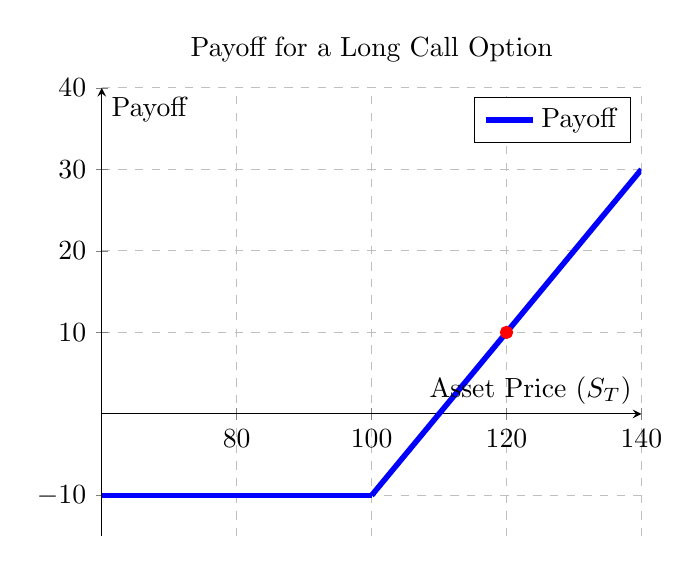
\begin{tikzpicture}
\begin{axis}[
    title={Payoff for a Long Call Option},
    xlabel={Asset Price (\( S_T \))},
    ylabel={Payoff},
    xmin=60, xmax=140,
    ymin=-15, ymax=40,
    axis lines=middle,
    grid=major,
    grid style=dashed,
]
\addplot[blue, thick,line width=2pt, domain=100:140]{max(0, x-100)-10};
\addplot[blue, thick,line width=2pt, domain=60:100]{-10};

%  add a dot to (120, 10)
\addplot[red, mark=*, thick] coordinates {(120, 10)};

\legend{Payoff}
\end{axis}
\end{tikzpicture}
\end{figure}

\subsection*{Short Call}

A short call option involves selling the call option, thus obligating the seller to sell the underlying asset at the strike price if the option is exercised. The payoff for a short call option is:
\[ \text{Payoff} = \min(0, K - S_T) + \text{premium} \]

\textbf{Example:} If a short call option with premium 10 and a strike price of \( K = 100 \) is exercised and the asset price is \( S_T = 120 \), the payoff is \( \min(0, 100 - 120) + 10 = -10 \).

\begin{figure}[H]
    \centering
    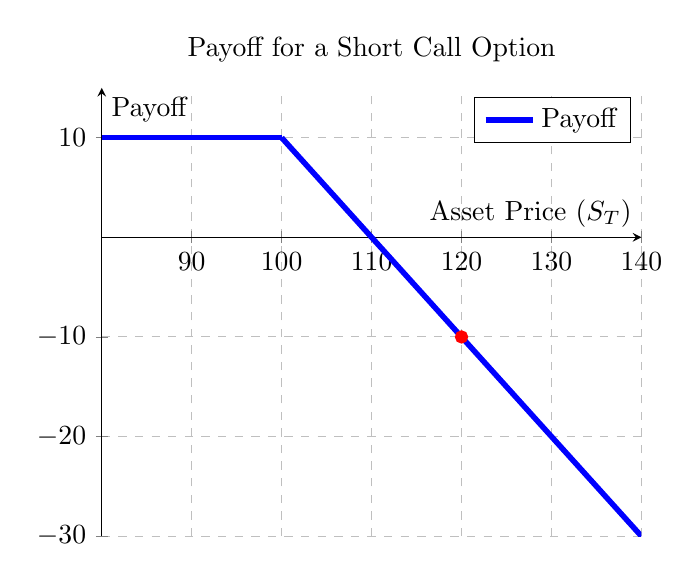
\begin{tikzpicture}
        \begin{axis}[
            title={Payoff for a Short Call Option},
            xlabel={Asset Price (\( S_T \))},
            ylabel={Payoff},
            xmin=80, xmax=140,
            ymin=-30, ymax=15,
            axis lines=middle,
            grid=major,
            grid style=dashed,
        ]
        \addplot[blue, thick,line width=2pt, domain=100:140]{min(0, 100-x)+10};
        \addplot[blue, thick,line width=2pt, domain=80:100]{10};
        \addplot[red, mark=*, thick] coordinates {(120, -10)};
        \legend{Payoff}
        \end{axis}
        \end{tikzpicture}
\end{figure}

\subsection*{Long Put}

A long put option gives the holder the right to sell the underlying asset at the strike price. The payoff for a long put option is:
\[ \text{Payoff} = \max(0, K - S_T) - \text{premium}\]

\textbf{Example:} For a long put option with a premium of 10 and a strike price of \( K = 100 \) and an asset price at maturity of \( S_T = 80 \), the payoff is \( \max(0, 100 - 80) -10 = 10 \).

\begin{figure}[H]
    \centering
    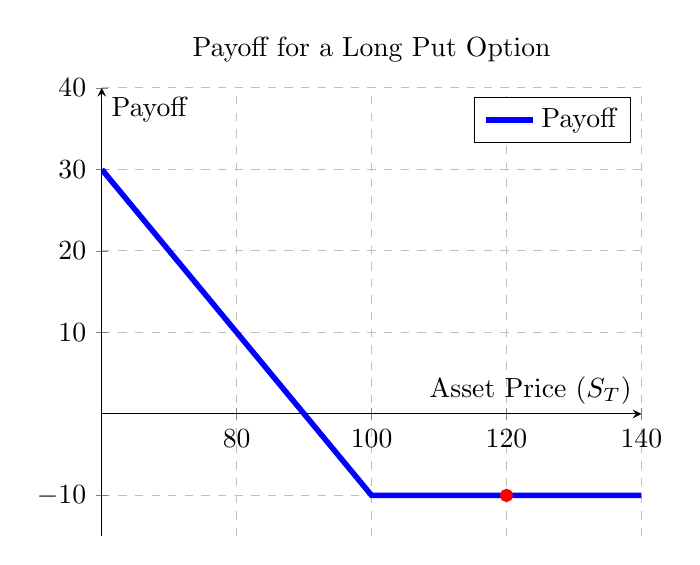
\begin{tikzpicture}
        \begin{axis}[
            title={Payoff for a Long Put Option},
            xlabel={Asset Price (\( S_T \))},
            ylabel={Payoff},
            xmin=60, xmax=140,
            ymin=-15, ymax=40,
            axis lines=middle,
            grid=major,
            grid style=dashed,
        ]
        \addplot[blue, thick,line width=2pt, domain=60:140]{max(0, 100-x)-10};
        \addplot[red, mark=*, thick] coordinates {(120, -10)};
        \legend{Payoff}
        \end{axis}
        \end{tikzpicture}
\end{figure}

\subsection*{Short Put}

A short put option involves selling the put option, obligating the seller to buy the underlying asset at the strike price if the option is exercised. The payoff for a short put option is:
\[ \text{Payoff} = \min(0, S_T - K) + \text{premium} \]

\textbf{Example:} If a short put option with a strike price of \( K = 100 \) is exercised and the asset price at maturity is \( S_T = 80 \), the payoff is \( \min(0, 80 - 100)  + 10= 10\).

\begin{figure}[H]
    \centering
    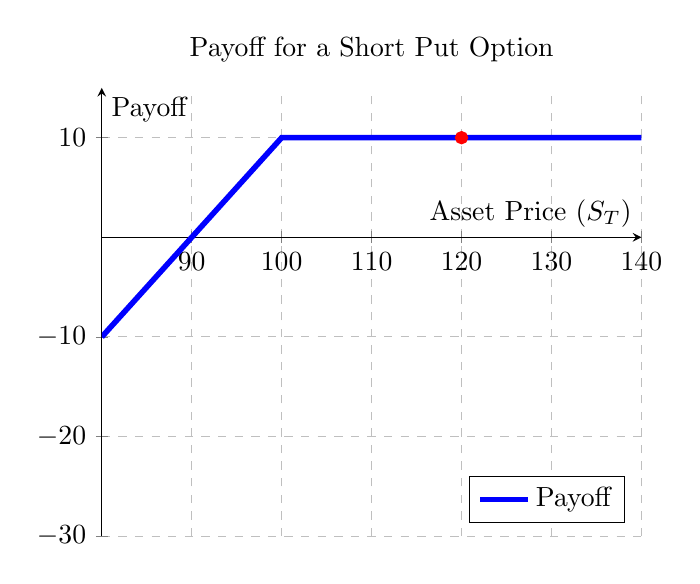
\begin{tikzpicture}
        \begin{axis}[
            title={Payoff for a Short Put Option},
            xlabel={Asset Price (\( S_T \))},
            ylabel={Payoff},
            xmin=80, xmax=140,
            ymin=-30, ymax=15,
            axis lines=middle,
            grid=major,
            grid style=dashed,
            legend pos = south east,
        ]
        \addplot[blue, thick, line width = 2pt, domain=80:140]{min(0, x-100) + 10};
        \addplot[red, mark=*, thick] coordinates {(120, 10)};


        \legend{Payoff}
        \end{axis}
        \end{tikzpicture}
\end{figure}

Out of all four cases, it was only the short put that had a positive payoff. 

\section{Binomial Option Pricing Model}

The Binomial Model assumes that in each period (time step), the return of the underlying asset can take one of two possible values.

\begin{figure}[H]
    \centering
    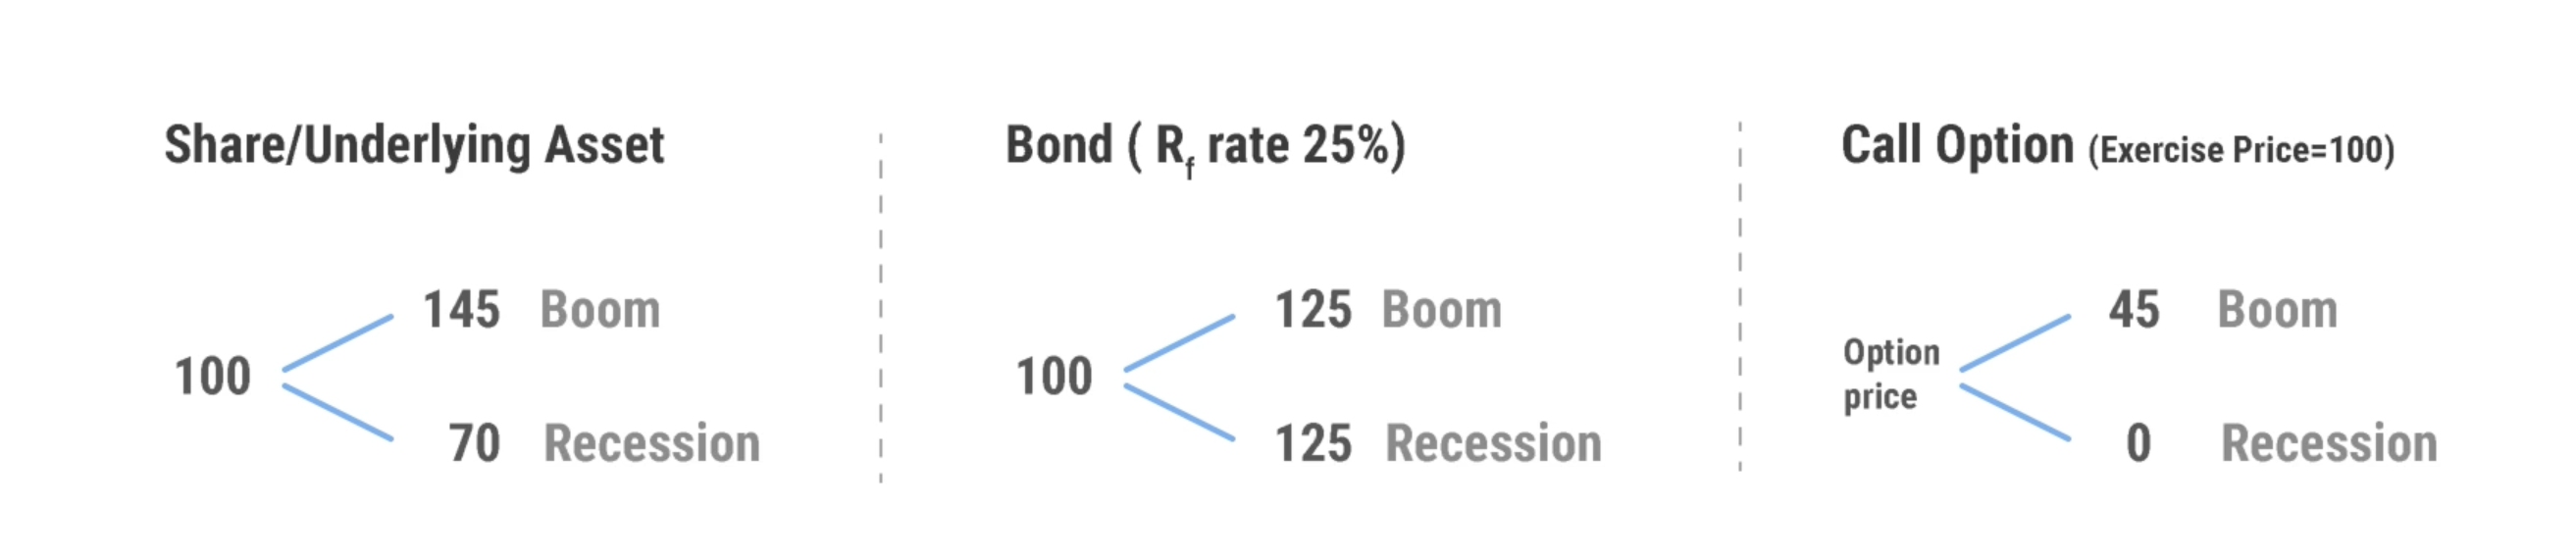
\includegraphics[width=0.9\textwidth]{img/9.4.1.png}
    \caption{Binomial valuation of options}
    \label{fig:binomial}
\end{figure}

\subsection*{Replication}
A replication strategy finds an investment in a combination of asset and risk-free bond (for calculation purposes, assume the bond is always risk-free) that replicates the call option's payoff at maturity.  To do this we need to determine the call option's delta, the number of shares needed in the replicating portfolio to replicate the option's payoff.

We have the following equations:

\begin{align}
    \text{Upwards movement in share price: } uS\Delta + (1+r_f)B &= C^{up}\\
    \text{Downwards movement in share price: } dS\Delta + (1+r_f)B &= C^{down}
\end{align}

\begin{itemize}
    \item Where \( u \) and \( d \) are the upward and downward multiplied movements in the share price, so $uS$ and $dS$ are the final share prices in the up and down states.
    \item \( S \) is the current share price,
    \item \( \Delta \) is the number of shares in the replicating portfolio,
    \item \( B \) is the amount invested in the risk-free bond,
    \item \( r_f \) is the risk-free rate, and
    \item \( C^{up} \) and \( C^{down} \) are the call option prices in the up and down states, respectively.
\end{itemize}

We can solve the equations to find the replicating portfolio's delta and the amount invested in the risk-free bond. From this point onwards, $r$ refers to the risk-free rate.

\begin{align}
    \Delta&=\frac{C^{up}-C_{\mathrm{down}}}{(u-d)S}\\
    B     &=\frac{uC_{\mathrm{down}}-dC^{up}}{(u-d)(1+r_f)}
\end{align}

The call option price $C$ is the delta times the share price plus the amount invested in the risk-free bond.

\begin{equation}
    C = S\Delta + B
\end{equation}

Solving the example in Figure \ref{fig:binomial}, we have:

\begin{align*}
    &\Delta=0.6 \\
    &B=-33.6 \\
    &C=0.6 \times 100 - 33.6 = 26.4
    \end{align*}

\subsection*{Risk-Neutral Model}

This stems from the replicating portfolio method, but also determines the risk-neutral probabilities of the two outcomes, for example, a boom or recession in the example of Figure \ref{fig:binomial}.\\

When these probabilities have been determined, we discount the expected payoff of the option at the risk-free rate.\\

The price of the call option can be expressed as the present value of the expected payoff,

\begin{equation}
    C = \frac{pC^{up}+(1-p)C^{down}}{r}
\end{equation}

Where $r$ is the risk-free rate and $p$ is the risk-neutral probability of the upward movement. $p$ is defined by:


\begin{equation}
    p = \frac{1+r-d}{u-d}
\end{equation}

Where:
\begin{itemize}
    \item \( r \) is the risk-free rate,
    \item \( u \) is the upward movement in the share price, and
    \item \( d \) is the downward movement in the share price.
\end{itemize}

In the example of Figure \ref{fig:binomial}, we have:
\begin{align}
    p=\frac{1.25-0.7}{1.45-0.7}=0.733\\
    1-p = 0.267
\end{align}

We can extend this model to a two-period example, reusing the values for $d$ and $u$.
\begin{figure}[H]
    \centering
    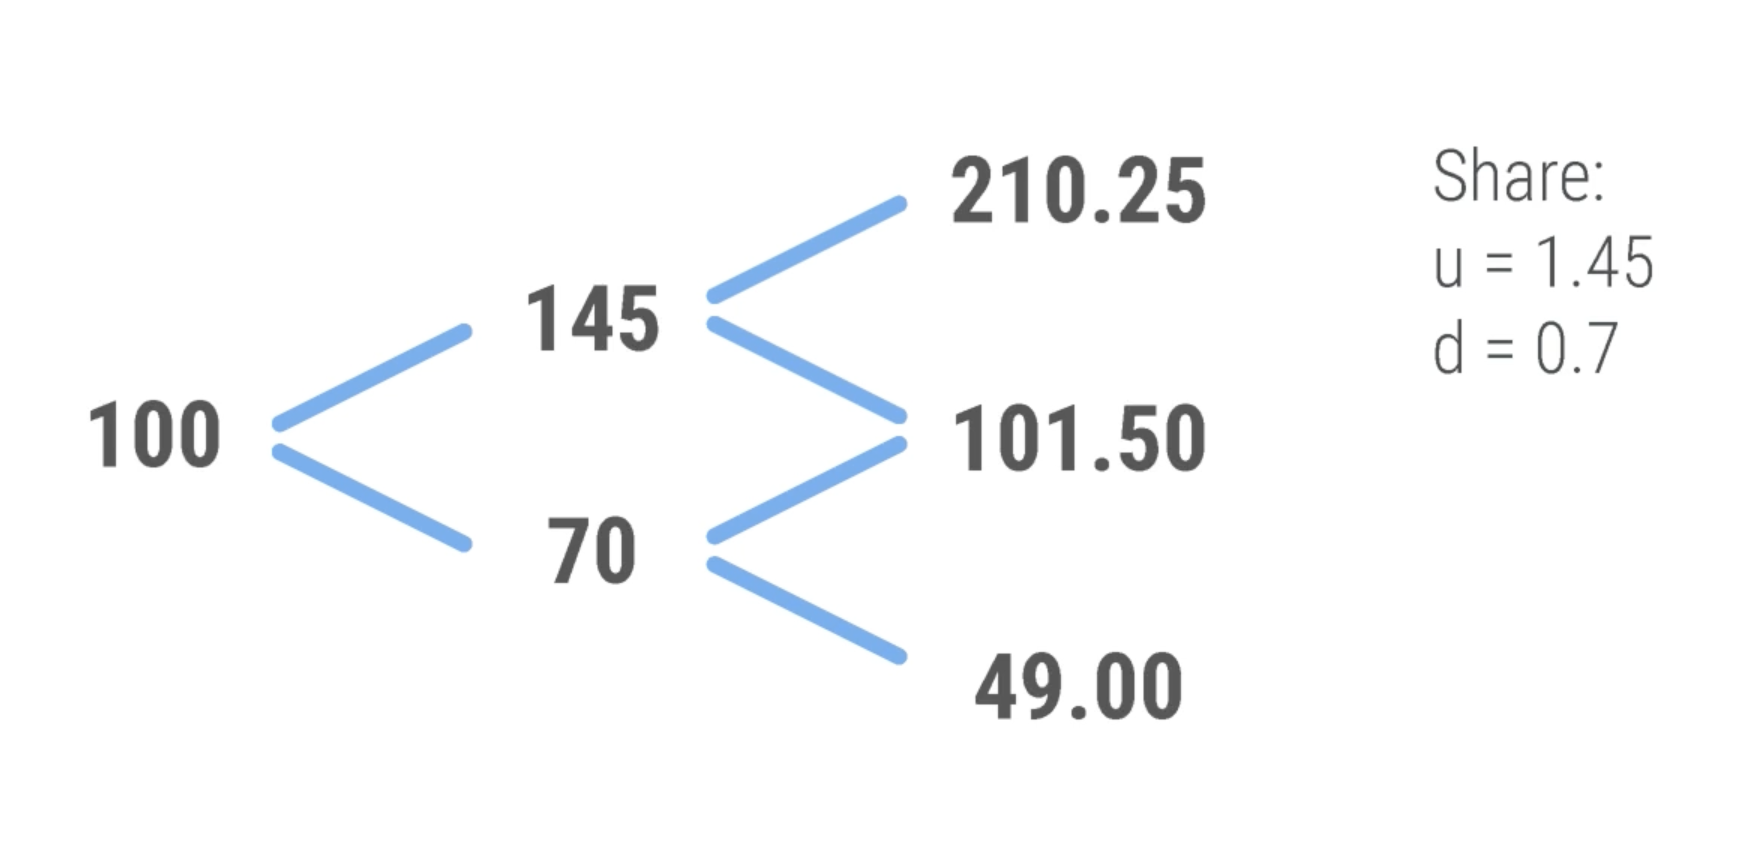
\includegraphics[width=0.5\textwidth]{img/9.4.2.png}
    \caption{Two-period binomial model (stock tree)}
    \label{fig:two-period}  
\end{figure}

In the case of only being provided only the final outcomes, it is non-trivial to determine the prices in different points in time, since the values of $u$ and $d$ are the same for every time step.

\begin{figure}[H]
    \centering
    \begin{subfigure}{0.48\textwidth}
        \centering
        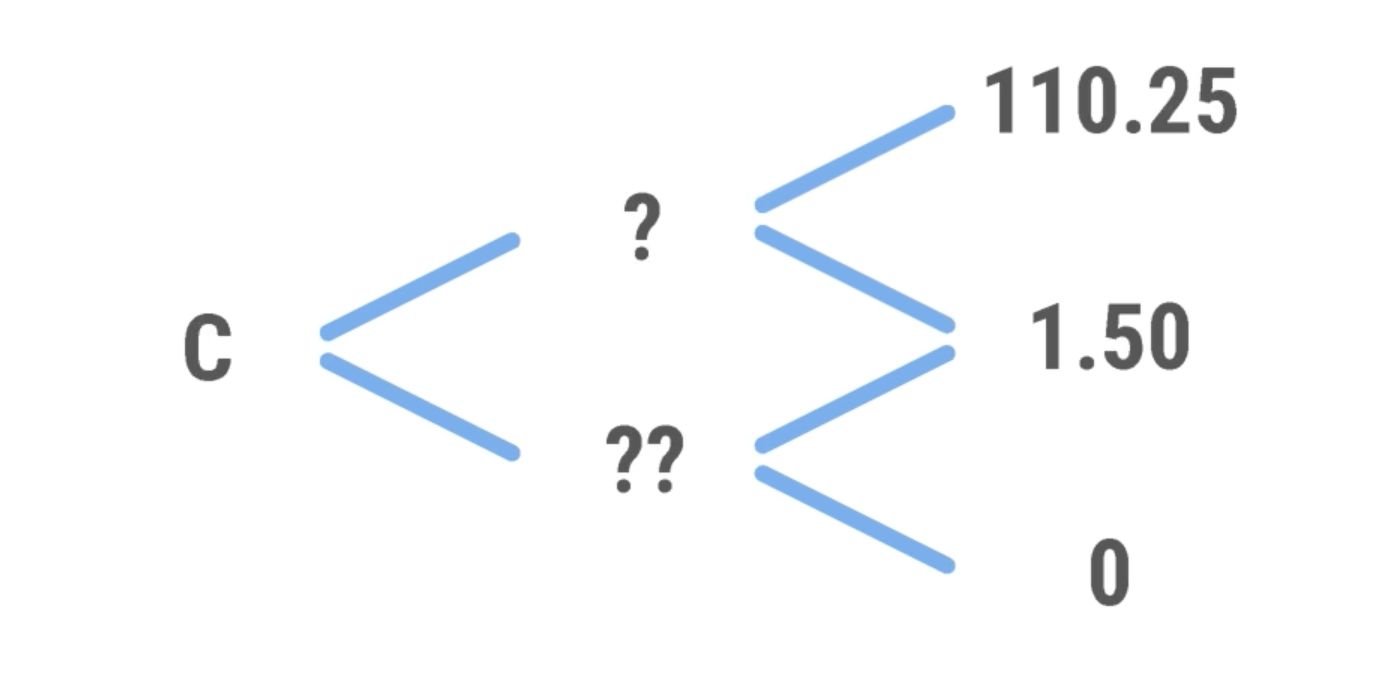
\includegraphics[width=0.5\textwidth]{img/9.4.3.png}
    \end{subfigure}
    \begin{subfigure}{0.48\textwidth}
        \centering
        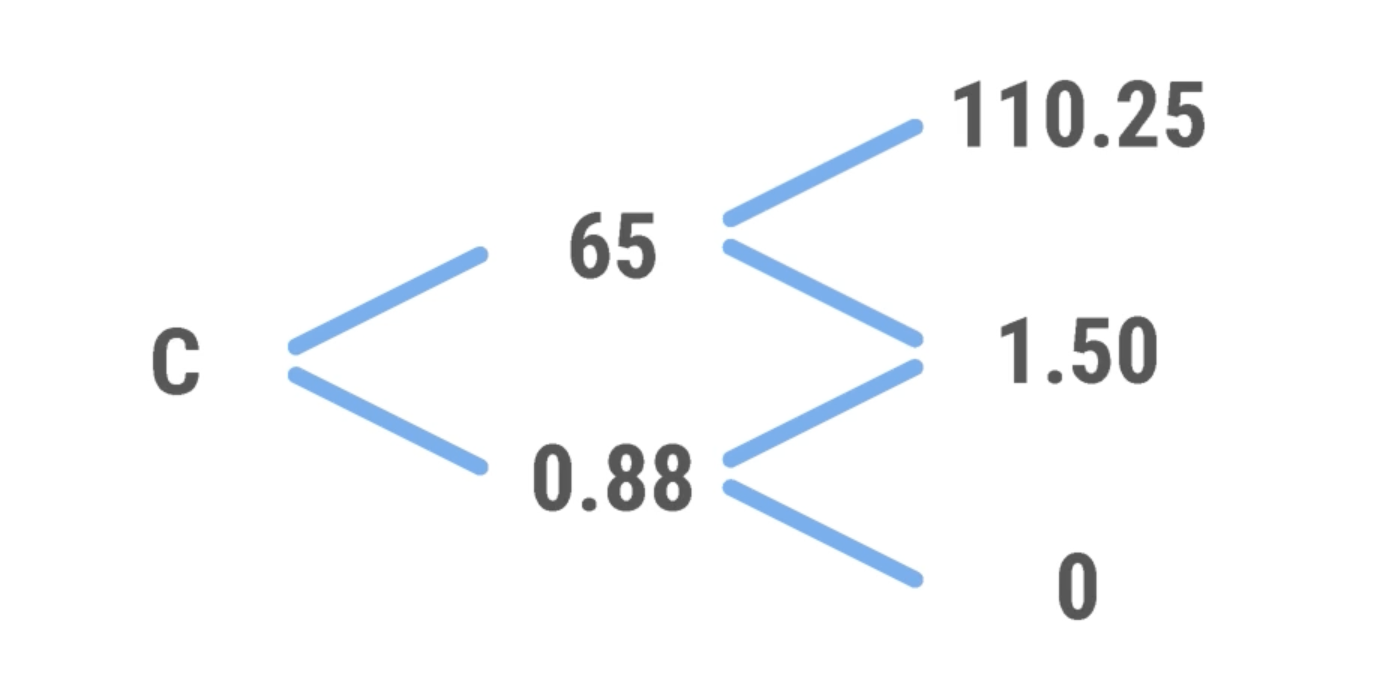
\includegraphics[width=0.5\textwidth]{img/9.4.4.png}
    \end{subfigure}
    \caption{Determining prices in a two-period binomial model (stock tree)}
\end{figure}

\subsection*{Put-Call Parity}
Put-call parity is a relationship between the price of a European call option and a European put option with the same strike price and expiry date. It is given by:

\begin{equation}
    C - P = S - Ke^{-rT}
\end{equation}
    
    Where:
    \begin{itemize}
        \item \( C \) is the price of the call option,
        \item \( P \) is the price of the put option,
        \item \( S \) is the current price of the underlying asset,
        \item \( K \) is the strike price of the options,
        \item \( r \) is the risk-free rate, and
        \item \( T \) is the time to maturity.
    \end{itemize}   



\begin{examplebox}{Options Questions}

\begin{figure}[H]
    \centering
    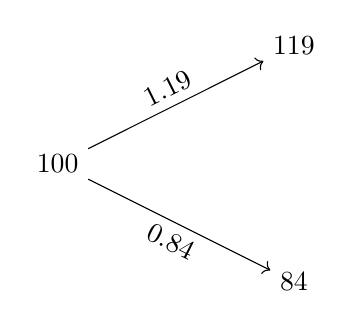
\begin{tikzpicture}[sloped]
        \node (a) at (0,0) {$100$};
        \node (b) at (3,-1.5) {$84$};
        \node (c) at (3,1.5) {$119$};

        
        \draw [->] (a) to node [below] {$0.84$} (b);
        \draw [->] (a) to node [above] {$1.19$} (c);
      \end{tikzpicture}
      \caption{Stock Tree}
\end{figure}

      
    \textbf{Question:} Over the next year, the price of stock W could increase by 19\% or go down by 16\%. Currently, the value of a stock is 100. The annual riskless interest rate is 4\%. What is the risk-neutral probability of the scenario (state) `up'?\\

\textbf{Answer:}
Using the formula for the risk-neutral probability:
\[
p = \frac{1 + r - d}{u - d}
\]
where \( r = 0.04 \) (risk-free rate), \( u = 1.19 \) (up movement), and \( d = 0.84 \) (down movement), we calculate:
\[
p = \frac{1.04 - 0.84}{1.19 - 0.84} = \frac{0.20}{0.35} \approx 0.57
\]

\textbf{Question:} What is the value of a European call option on a share of company W, with an exercise price of 90 and time to maturity of 1 year?\\

\textbf{Answer:}
Assuming that the strike price \( K = 90 \), and using the previously calculated risk-neutral probability \( p = 0.57 \), the values in the up and down state at maturity would be:
\[
C^{up} = \max(0, 1.19 \times 100 - 90) = 29
\]
\[
C^{down} = \max(0, 0.84 \times 100 - 90) = 0
\]

The option will not be exercised at the down state as 84 is less than 90. So the option value is 0. Using the equation:
\begin{equation}
    C = \frac{pC^{up}+(1-p)C^{down}}{r}
\end{equation}

We work out the option's current value to be:
\[
C = \frac{0.57 \times 29 + 0.43 \times 0}{1.04} \approx 15.894
\]

\begin{figure}[H]
    \centering
    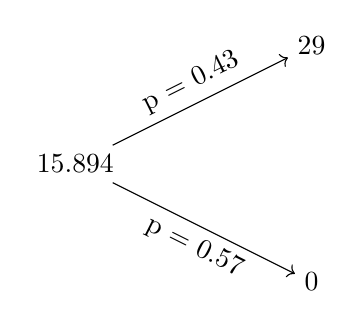
\begin{tikzpicture}[sloped]
        \node (a) at (0,0) {$15.894$ };
        \node (b) at (3,-1.5) {$0$};
        \node (c) at (3,1.5) {$29$};

        
        \draw [->] (a) to node [below] {p = 0.57} (b);
        \draw [->] (a) to node [above] {p = 0.43} (c);
      \end{tikzpicture}
      \caption{Call Tree}
\end{figure}

The option value \( C \) is then:
\[
C = \frac{0.57 \times 29 + 0.43 \times 0}{1.04} \approx 15.894
\]

\textbf{Question:} Based on put-call parity, compute the value of a put option on stock W, with time to maturity of 1 year and a strike price of 90.\\

\textbf{Answer:}
Using put-call parity:
\[
P = C + Ke^{-rT} - S
\]
Substituting the values:
\[
P = 15.894 + 90e^{-0.04 \times 1} - 100
\]
\[
P \approx 2.37
\]

\textbf{Question:} Determine the value of a put option on stock W with time to maturity of 2 years and an exercise price of 90.\\

\textbf{Answer:}
This question requires extending the binomial model to two periods. To fill in the 1st period on the call tree, use the equation:

\begin{equation}
    C = \frac{pC^{up}+(1-p)C^{down}}{r}
\end{equation}

\begin{figure}[H]
    \centering
    \begin{subfigure}[b]{0.48\textwidth}
        \centering
        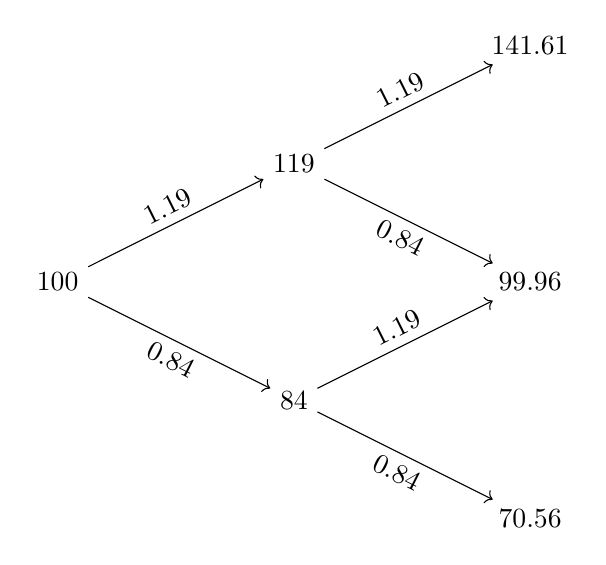
\begin{tikzpicture}[sloped]
            \node (a) at (0,0) {$100$};
            \node (b) at (3,-1.5) {$84$};
            \node (c) at (3,1.5) {$119$};
            \node (d) at (6,-3) {$70.56$};
            \node (e) at (6,0) {$99.96$};
            \node (f) at (6,3) {$141.61$};
            
            \draw [->] (a) to node [below] {$0.84$} (b);
            \draw [->] (a) to node [above] {$1.19$} (c);
            \draw [->] (c) to node [below] {$0.84$} (e);
            \draw [->] (c) to node [above] {$1.19$} (f);
            \draw [->] (b) to node [below] {$0.84$} (d);
            \draw [->] (b) to node [above] {$1.19$} (e);
        \end{tikzpicture}
        \caption{Stock Tree}
    \end{subfigure}
    \begin{subfigure}[b]{0.48\textwidth}
        \centering
        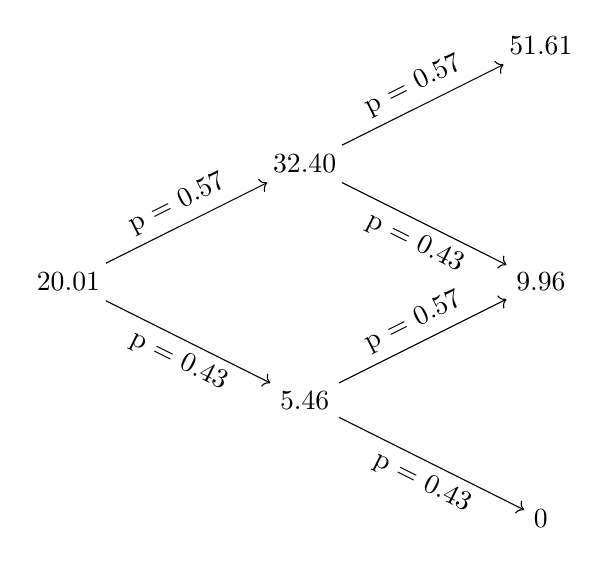
\begin{tikzpicture}[sloped]
            \node (a) at (0,0) {$20.01$};
            \node (b) at (3,-1.5) {$5.46$};
            \node (c) at (3,1.5) {$32.40$};
            \node (d) at (6,-3) {$0$};
            \node (e) at (6,0) {$9.96$};
            \node (f) at (6,3) {$51.61$};
            
            \draw [->] (a) to node [below] {p = 0.43} (b);
            \draw [->] (a) to node [above] {p = 0.57} (c);
            \draw [->] (c) to node [below] {p = 0.43} (e);
            \draw [->] (c) to node [above] {p = 0.57} (f);
            \draw [->] (b) to node [below] {p = 0.43} (d);
            \draw [->] (b) to node [above] {p = 0.57} (e);
        \end{tikzpicture}
        \caption{Call Tree}
    \end{subfigure}
    \caption{Stock and Call Trees}
\end{figure}

The risk-neutral probability of the up state is:
\[
p = \frac{1.04 - 0.84}{1.19 - 0.84} = \frac{0.20}{0.35} \approx 0.57
\]
\[
    1-p =  0.43
\]

The value of the call option with time to maturity of 2 years and an exercise price of 90 is:
\[
P = \frac{(51.61 \times 0.57^2 )+ (9.96 \times 0.57 \times 0.43) + (9.96 \times 0.43 \times 0.57)}{1.04^2} = 20.01
\]

Using put-call parity to determine the value of the put option:
\[
P = C + Ke^{-rT} - S = 20.01 + 90e^{-0.04 \times 2} - 100 \approx 3.09
\]



\end{examplebox}
\chapter{Risk Management: Options and Corporate Finance}

\section{Introduction}

Topics:
\begin{itemize}
    \item Describe the basics of using options in risk management
    \item Identify what drives the value of options (intrinsic and speculative values)
    \item Examine the different strategies to build funds, including options
\end{itemize}

\section{Equity and Debt as Options}

\begin{itemize}
    \item Options provide valuable insights into corporate finance concepts, particularly in understanding debt and equity.
    \item \textbf{Equity} can be conceptualised as a \textbf{long call option on a firm's assets} with a strike price equivalent to the value of debt:
      \begin{itemize}
        \item If the firm's value exceeds the debt, equity holders benefit from the residual value post-debt repayment.
        \item If not, equity holders lose their investment, similar to an option expiring worthless.
      \end{itemize}
      \begin{figure}[H]
        \centering
        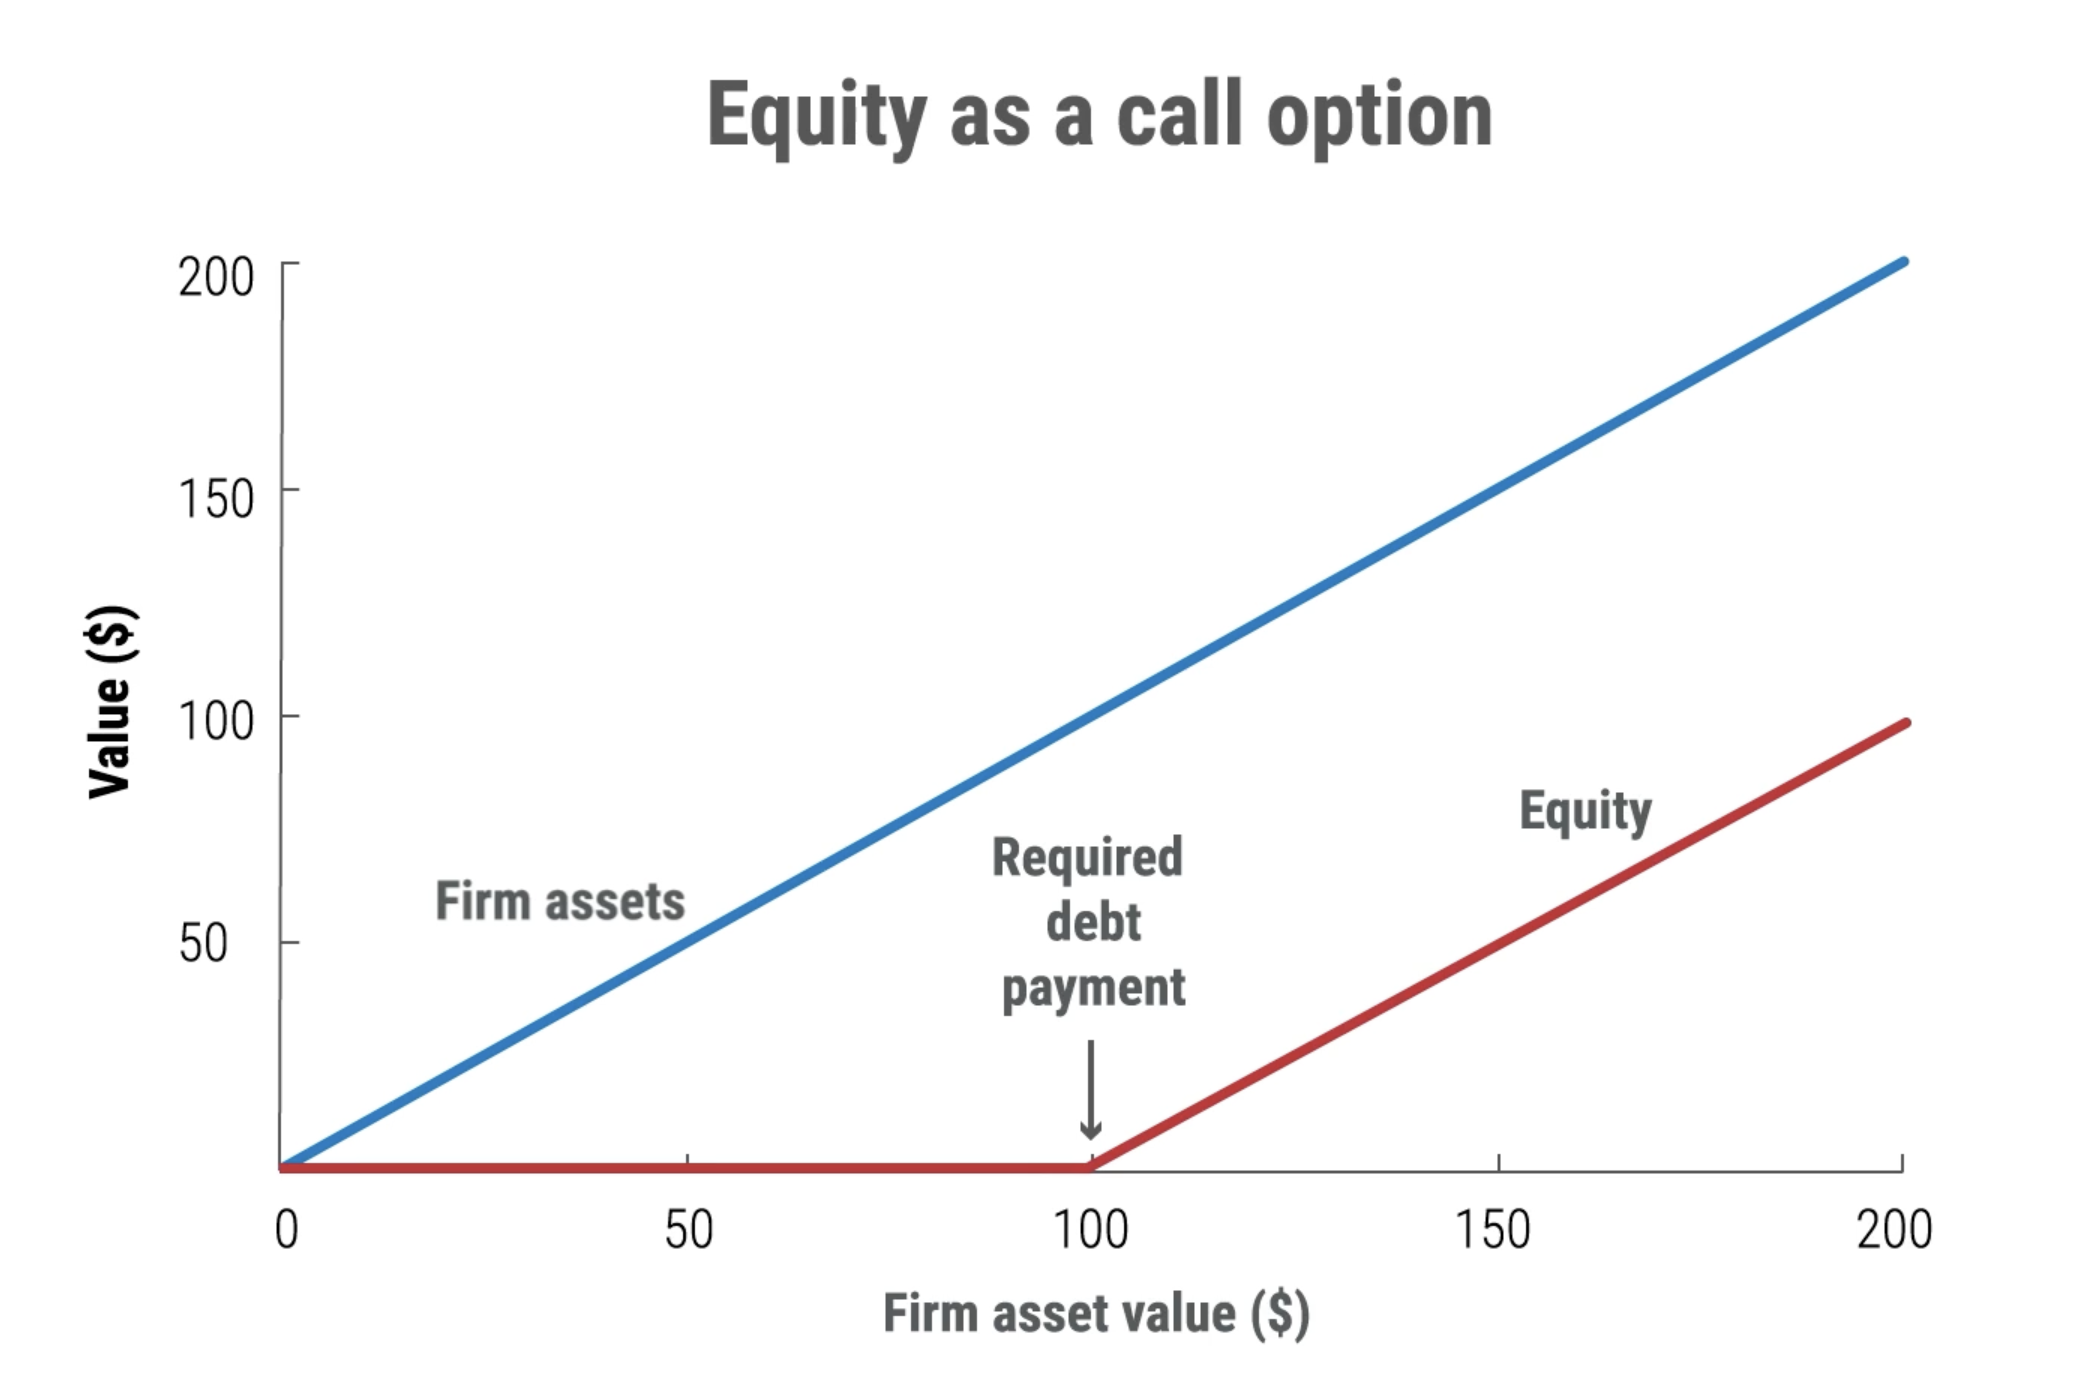
\includegraphics[width=0.5\textwidth]{img/10.2.1.png}
        \caption{Equity as a Call Option}
        \end{figure}
    \item Equity shares resemble call options in several ways:
      \begin{itemize}
        \item They offer limited risk, capping potential losses to the initial investment.
        \item They provide unlimited upside, allowing equity holders to benefit fully from increases in the firm's value.
        \item Unlike traditional options, equity does not expire, permitting long-term value appreciation.
      \end{itemize}
    \item \textbf{Debt} can also be analysed using options theory:
      \begin{itemize}
        \item It can be seen as a \textbf{short put option on the firm's assets with a strike price equal to debt}.
        \item If asset values fall below the debt level, the put option is exercised, leaving debt holders with the firm's remaining assets.
        \item If asset values exceed the debt, debt holders receive only the debt amount, similar to a call option's strike price being met.
      \end{itemize}
      \begin{figure}[H]
        \centering
        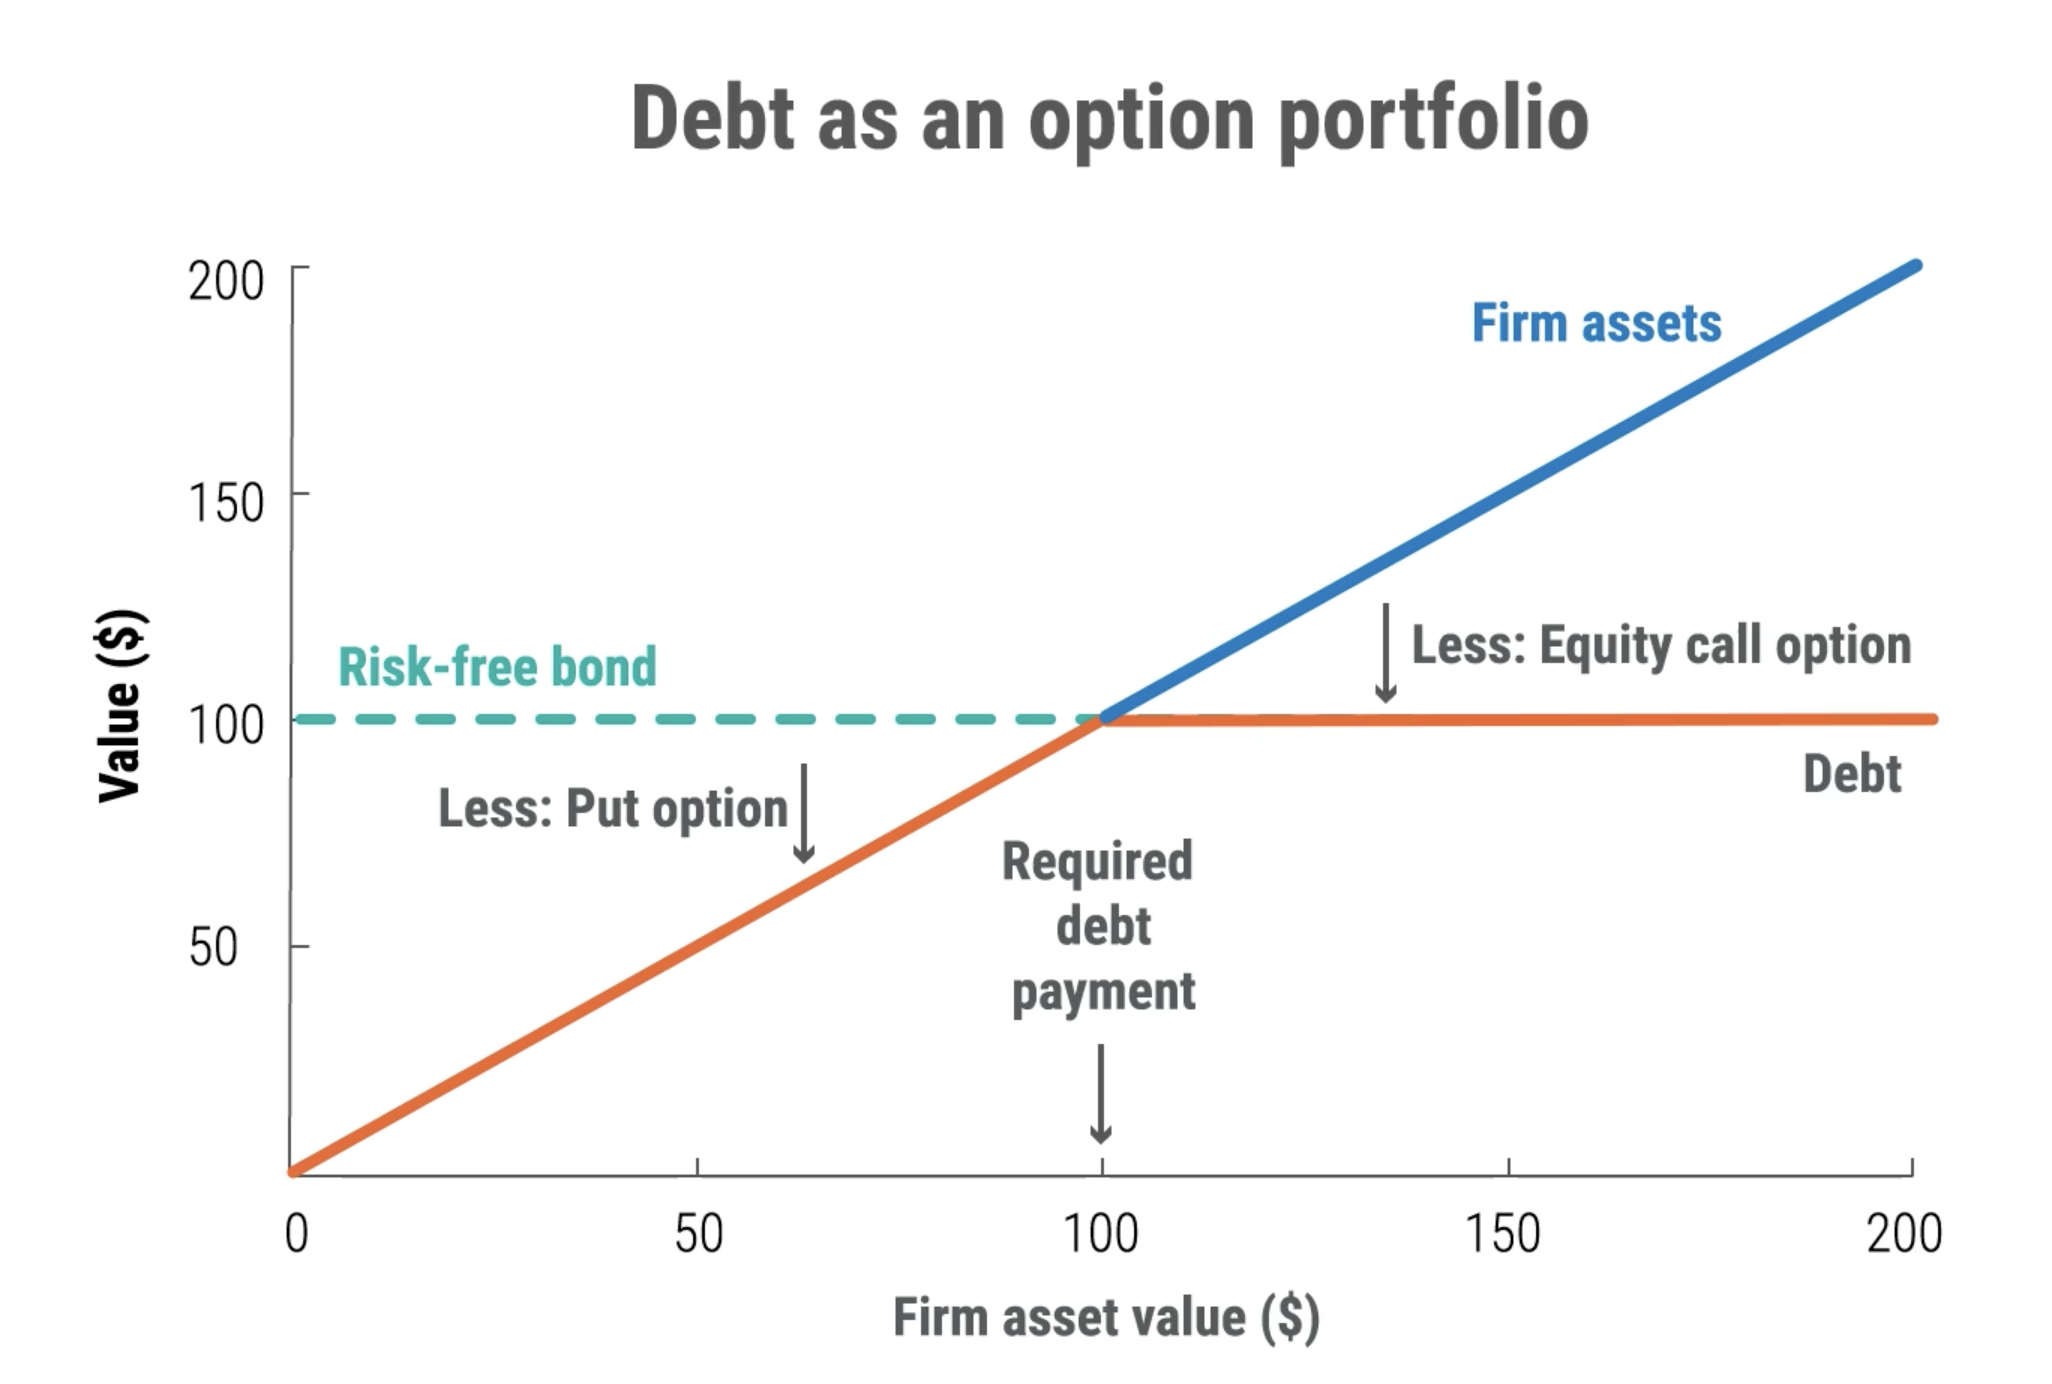
\includegraphics[width=0.5\textwidth]{img/10.2.2.png}
        \caption{Debt as a Put Option}
        \end{figure}
  \end{itemize}
  
\section{Agency Conflict}
\subsection*{Debt Equity Considered as Options}

% \begin{itemize}
%     \item Viewing debt equity as options provides a methodological framework for pricing securities.
%     \item Useful in situations where a company has traded options but no outstanding debt, assisting in pricing a debt issue.
%     \item The option characterisation of debt and equity securities offers a new perspective on agency conflicts between equity holders and debt holders.
%     \item These conflicts may lead to:
%     \begin{itemize}
%         \item Overinvestment or underinvestment issues.
%         \item Divergent attitudes towards risk due to equity's similarity to a call option:
%         \begin{itemize}
%             \item Equity holders benefit from risky investments, reflecting a preference for higher risk (akin to holding a long call option).
%             \item Conversely, this positions equity holders similarly to short put option holders, where increased risk is detrimental.
%         \end{itemize}
%     \end{itemize}
%     \item Such dynamics can lead to an over-investment problem:
%     \begin{itemize}
%         \item New investments that enhance asset values can decrease the value of the effective short put held by equity holders.
%         \item This reduction in put value means that some benefits of asset value increase are transferred to debt holders, diminishing equity holders' incentives to invest.
%     \end{itemize}
%     \item The shift in incentives can result in:
%     \begin{itemize}
%         \item A debt overhang, where the potential gains from new investments accrue more to debt holders than to equity holders.
%         \item An underinvestment problem, as equity holders perceive reduced benefits from investment.
%     \end{itemize}
% \end{itemize}


\begin{itemize}
    \item Thinking of debt and equity as options can help price securities, especially when a company has traded options but no debt outstanding. This is because options pricing models can be used to estimate the value of debt and equity, providing a more accurate picture of a company's capital structure.
    \item This perspective provides a new interpretation of agency conflicts between equity holders and debt holders. By recognizing that debt and equity have option-like characteristics, we can better understand the incentives and conflicts that arise between these two groups.
    \item Equity can be viewed as a call option, giving equity holders a potential upside from investments. This is because equity holders benefit from any increase in the firm's value, making their claim on the firm's assets more valuable.
    \item However, debt holders have a short put option position, which means they are hurt by increased risk. This is because debt holders are obligated to receive a fixed return, and any increase in risk reduces the value of their claim on the firm's assets.
    \item This can lead to:
        \begin{itemize}
            \item Overinvestment: Equity holders may take on excessive risk, as they benefit from potential gains and have limited liability. This can lead to a moral hazard problem, where equity holders take on too much risk at the expense of debt holders.
            \item Underinvestment: Debt holders may be hesitant to invest, as increased risk reduces the value of their put option. This can lead to a debt overhang problem, where debt holders are reluctant to provide financing for new projects.
        \end{itemize}
    \item When a firm makes new investments, the value of the debt (short put option) increases, as the assets backing the debt become more valuable. This means that debt holders benefit from the increased asset value, as their claim on the firm's assets becomes more secure.
    \item When debt holders benefit from increased asset value, equity holders may be less inclined to invest in new projects, as the benefits of those investments may accrue primarily to debt holders. This can lead to a debt overhang problem, where equity holders are hesitant to invest in projects that could increase the firm's value.y be less inclined to invest, as they may not capture the full benefits of their investments. This is known as the debt overhang problem or underinvestment problem, where equity holders may be hesitant to invest in projects that could increase the value of the firm, as the benefits may accrue to debt holders instead.
\end{itemize}

\section{Pricing Risky Debt}


As of December 2014, Apple Inc. has no long-term debt. The market capitalisation of Apple as of December 2014 is \$616 billion, which corresponds to a share price of \$110. Assume that in January 2015 Apple plans to issue \$336 billion (face value) of new corporate debt, as part of a leverage recap. Assume this debt to be zero coupon debt, maturing in January 2017. The risk-free bonds with similar maturity offer a 0.4\% return.

\begin{table}[htbp]
    \centering
    \caption{Call and Put Option Prices of Apple's shares with Jan 2017 Maturity}
    \label{tab:option-prices}
    \begin{tabular}{ccc|ccc}
    \toprule
    \multicolumn{3}{c|}{CALLS} & \multicolumn{3}{c}{PUTS} \\ 
    \midrule
    \textbf{Strike} & \textbf{Price} & & \textbf{Strike} & \textbf{Price} & \\
    \midrule
    50  & 62.1  & & 50  & 0.95  & \\
    55  & 57.5  & & 55  & 1.19  & \\
    \textbf{60}  & \textbf{52.5 } & & 60  & 2.05  & \\
    65  & 48.1  & & 65  & 2.85  & \\
    70  & 50.25 & & 70  & 4.85  & \\
    75  & 41.15 & & 75  & 4.95  & \\
    80  & 39    & & 80  & 6     & \\
    85  & 32.2  & & 85  & 7.75  & \\
    87.5& 34.25 & & 87.5& 8.3   & \\
    90  & 33.75 & & 90  & 8     & \\
    92.5& 30.18 & & 92.5& 10.81 & \\
    95  & 25    & & 95  & 11.55 & \\
    97.5& 26.37 & & 97.5& 13    & \\
    100 & 25.3  & & 100 & 13.76 & \\
    105 & 23.17 & & 105 & 16.45 & \\
    110 & 20    & & 110 & 19.15 & \\
    115 & 17    & & 115 & 22    & \\
    120 & 16.82 & & 120 & 25.3  & \\
    125 & 14.62 & & 125 & 28.56 & \\
    130 & 13.55 & & 130 & 32.25 & \\
    135 & 11    & & 135 & 32.5  & \\
    140 & 10.5  & & 140 & 37.72 & \\
    145 & 9.35  & & 145 & 42.5  & \\
    150 & 8.55  & & 150 & 45.25 & \\
    155 & 7.4   & & 155 & 51.29 & \\
    160 & 6.6   & & 160 & 53.5  & \\
    165 & 6.01  & & 165 & 59.25 & \\
    170 & 5.51  & & 170 & 57.75 & \\
    175 & 4.76  & & 175 & 64.25 & \\
    \bottomrule
    \end{tabular}
    \end{table}
    
\textbf{Question 1: }
How many shares outstanding does Apple have?
\textbf{Answer: }
The market capitalisation of Apple is \$616 billion, and the share price is \$110. Therefore, the number of shares outstanding is $616B/110 = 5.6B$ shares.\\

\textbf{Question 2: }
Assuming perfect capital markets, what should be the market value of the firm (equity plus debt) after the recap?
\textbf{Answer: }
Since assuming perfect capital markets (Modigliani and Miller Preposition 1), the value of the firm after the recap should be the same as before the recap. Therefore, the market value of the firm after the recap should be \$616 billion.


\begin{itemize}
    \item Market Capitalisation: \$616 billion
    \item Share Price: \$110
    \item Shares Outstanding: 5.6 billion
    \item Debt Issuance: \$336 billion (zero coupon)
    \item Maturity: January 2017
    \item Risk Free Rate: 0.4\%
\end{itemize}


\textbf{Question 3: }
Assuming perfect capital markets, and taking into account the information on options being traded on Apple stock, what should be the market value of equity? What about the market value of debt?
\textbf{Answer: }
\begin{itemize}
    \item The debt issuance is equal to a claim of \$336 billion/5.6 billion shares = \$60 per share. 
    \item Because Apple's shareholders will receive only the value in excess of this debt claim, the value of Apple's equity after the recap is equal to the current value of the call option with strike price \$60.
    \item A call option for strike \$60 has a value of approximately \$52.5.
    \item Multiplying by the total number of shares, the total value of Apple's equity after the recap is \$52.5 $\times$ 5.6 billion = \$294 billion.
    \item To calculate the value of the new debt, we subtract this equity value from the total existing market capitalisation: \$616 billion - \$294 billion = \$322 billion.
\end{itemize}



\textbf{Question 3: }
What is the implied credit spread for Apple?
\textbf{Answer: }
\begin{itemize}
    \item As this debt matures in January 2017, this is 24 months away. The risk-free rate is 0.4\%, so this corresponds to a yield to maturity of:
    \item \begin{equation}
        \text{Yield to Maturity} = \left(1 + \frac{336}{322}\right)^{12/24} - 1 = 2.15\%
    \end{equation}
    \item Subtracting the risk-free-rate of 0.4\%, the credit spread is \textbf{1.75}\%.
\end{itemize}

\section{Real Options}
\subsection*{What are Real Options?}

Real options are a strategic decision-making framework that considers the flexibility and choices available when evaluating investments or projects. Unlike traditional financial methods, real options take into account the dynamic and uncertain nature of modern business environments.

\begin{itemize}
    \item Inspired by financial options (call and put options)
    \item Refer to managerial flexibility to make decisions in the future based on evolving business environments
    \item Include options to invest, delay, expand, abandon, or switch to a different technology
\end{itemize}

\subsection*{Types of Real Options}

\begin{itemize}
    \item \textbf{Option to Invest (Timing Option):} Decide when to make an investment based on evolving market conditions
    \item \textbf{Option to Delay (Flexibility Option): }Postpone investment until there's more clarity
    \item \textbf{Option to Expand (Growth Option):} Invest incrementally based on the success of an initial phase
    \item \textbf{Option to Switch Technology (Switch Option): }Switch between two different technologies or inputs based on observed market conditions
    \item \textbf{Option to Abandon (Shut Down Option): }Exit a project if it's not meeting expectations or if external conditions change
\end{itemize}

\subsection*{Limitations of Traditional Financial Analysis Methods}

Traditional financial analysis methods, such as Net Present Value (NPV) and Discounted Cash Flow (DCF), often overlook real options due to their simplifying assumptions.

\begin{itemize}
    \item Assume a static and deterministic world, ignoring flexibility and uncertainty
    \item Ignore the value of flexibility, such as delaying, expanding, or abandoning a project
    \item Fail to address uncertainty, using a single set of assumptions and discount rates
    \item Underestimate strategic value, neglecting the value of choices themselves
\end{itemize}

\begin{examplebox}{Real Options Question}
    Mrs Jones, the CEO of JJ Enterprise is considering expanding the business of her company. She could invest \$5 million today in a new plant that would double her current capacity. If she invests today, the plant will be ready to produce and generate cash flows by the end of year two that will last forever. The cash flows generated by the new plant will depend on how the economy is doing at the end of this year. If the economy has fully recovered, demand will be set high, and the plant will be expected to generate annual cash flows of \$0.6 million. If the economy is doing poorly, demand will be set low, and the plant will be expected to generate annual cash flows of only \$0.2 million. \\

    The probability that the economy fully recovers by the end of this year is 0.5.
    If we assume no taxes, no inflation and an appropriate discount rate of 10\%, the Net Present Value (NPV) of this project can be calculated as follows:


    \begin{figure}[H]
    \centering
    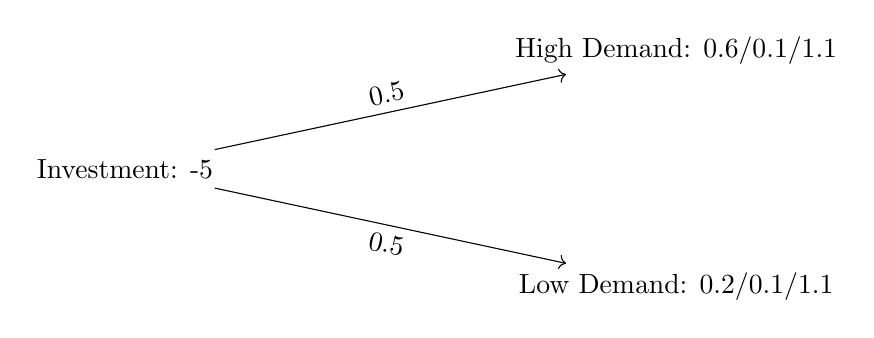
\begin{tikzpicture}[sloped]
        % Node definitions
        \node (a) at (0,0) {Investment: -5};
        \node (b) at (7,-1.5) {Low Demand: 0.2/0.1/1.1};
        \node (c) at (7,1.5) {High Demand: 0.6/0.1/1.1};

        % Edge definitions
        \draw [->] (a) to node [below] {0.5} (b);
        \draw [->] (a) to node [above] {0.5} (c);
    \end{tikzpicture}
    \caption{Option Tree for Investment Decision}
    \label{fig:option-tree}
    \end{figure}

    \textbf{Question: }
    What is the NPV? Should the CEO invest?\\
    \textbf{Answer: }
    \begin{align*}
        \text{NPV} &= -5 + 0.5 \times \left(\frac{0.6}{0.1 \times 1.1} \right) + 0.5 \times \left(\frac{0.2}{0.1 \times 1.1} \right) \\
        &= -1.36
    \end{align*}
    Negative NPV, so the CEO should not invest.\\

    \textbf{Question: }
    Now assume that the CEO has the option to delay the investment by one year to learn about demand levels, and can then decide whether or not to build the new plant. If she decides to wait one year to invest, the plant will only start to generate cash flows at the end of the third year. \\

    What is the new NPV and what is the value of the option to delay?

    \begin{figure}[H]
        \centering
        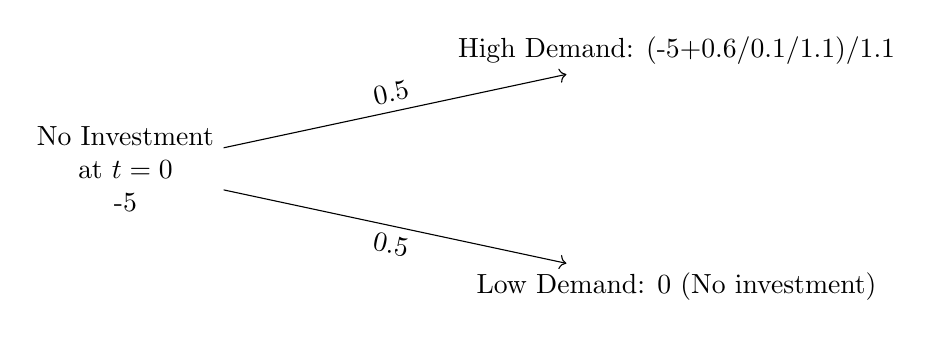
\begin{tikzpicture}[sloped]
            % Node definitions
            \node[align=center] (a) at (0,0) {No Investment \\ at $t=0$\\-5};
            \node (b) at (7,-1.5) {Low Demand: 0 (No investment)};
            \node (c) at (7,1.5) {High Demand: (-5+0.6/0.1/1.1)/1.1};
    
            % Edge definitions
            \draw [->] (a) to node [below] {0.5} (b);
            \draw [->] (a) to node [above] {0.5} (c);
        \end{tikzpicture}
        \caption{Option Tree for Investment Decision}
        \label{fig:option-tree-2}
    \end{figure}

    \textbf{Answer: }
    \begin{align*}
        \text{NPV} &= 0.5 \times \left(\frac{0.6}{0.1 \times 1.1} - 5\right) \\
        &= 0.207
    \end{align*}
    The value of the option to delay is $ 0.207 - (-1.36) = -1.57$.



\end{examplebox}



\end{document}

